%%%%%%%%%%%%%%%%%%%%%%%%%%%%%%%%%%%%%%
%%  NewMathSample.tex
%%  Sample file for New Math Style
%%  MIT Press
%%  May 21,2016
%%  Written by Amy Hendrickson
%%  amykaren@mit.edu
%%%%%%%%%%%%%%%%%%%%%%%%%%%%%%%%%%%%%%

\documentclass[6x9]{newmath}
\usepackage[utf8]{inputenc}
\usepackage{braket}
\usepackage{amssymb}
\usepackage[
type={CC},
modifier={by-sa},
version={4.0},
]{doclicense}

%%%%%%%%%%%%%%%%%%%%%%%%%%%%%%%%%%%%%%%%%%%%%%%%%%%%%%%%
% rwd-quantum : helpful macros for writing about quantum theory
%
%
% Inner products bras kets etc 
%
%\newcommand{\bra}[1]{%  dirac 'bra'
%    \ensuremath{\left\langle #1 \right|}\xspace}

%\newcommand{\ket}[1]{%  dirac 'ket'
%    \ensuremath{\left|  #1 \right\rangle}\xspace}

\newcommand{\innp}[2]{%  dirac style inner product
    \ensuremath{\langle #1 \mid #2 \rangle}}

\newcommand{\outp}[2]{%  dirac style outer product
    \ensuremath{\left|\left. #1 \rangle\right.\!\langle\left. #2 \right|\right. }}

\newcommand{\norm}[1]{% define command to get spacing right
        \ensuremath{\left| #1 \right| }}

%\newcommand{\braket}[2]{\ensuremath{\langle #1|#2 \rangle}}
\newcommand{\ketbra}[2]{\ensuremath{|#1 \rangle \langle #2|}}
\newcommand{\ro}[1]{\ensuremath{|#1 \rangle \langle #1|}}
\newcommand{\av}[1]{\ensuremath{\langle #1 \rangle}}
\newcommand{\real}{\ensuremath{\mathrm{Re}}}
\newcommand{\trace}{\ensuremath{\textsf{Tr}}}

%% use the proper notation for CZ etc
\newcommand{\CZ}{\ensuremath{\wedge Z}\xspace}
\newcommand{\CX}{\ensuremath{\wedge X}\xspace}
\newcommand{\CNot}{\CX}
\newcommand{\cnot}{\textsc{cnot}\xspace}
\newcommand{\ccnot}{\textsc{ccnot}\xspace}

\newcommand{\PsiPlus}{\ensuremath{\ket{\Psi^+}}\xspace}
\newcommand{\PsiMinus}{\ensuremath{\ket{\Psi^-}}\xspace}
\newcommand{\PhiPlus}{\ensuremath{\ket{\Phi^+}}\xspace}
\newcommand{\PhiMinus}{\ensuremath{\ket{\Phi^-}}\xspace}

\newcommand{\sulPisP}{\ensuremath{\bra{\Psi^+}}\xspace}
\newcommand{\suniMisP}{\ensuremath{\bra{\Psi^-}}\xspace}
\newcommand{\sulPihP}{\ensuremath{\bra{\Phi^+}}\xspace}
\newcommand{\suniMihP}{\ensuremath{\bra{\Phi^-}}\xspace}

% useful operator names
% trace
\newcommand{\Tr}{\operatorname{Tr}}
% probability
\newcommand{\Prob}{\operatorname{Pr}}
% projection operator 
% \newcommand{\Proj}{\operatorname{P}}

%%%%%%%%%%%%%%%%%%%%%%%%%%%%%
% visible editing comments in the PDF, per writer.

\newboolean{ShowComments}
\setboolean{ShowComments}{true}  % change to true to show remaining colorful author comments. 
                                 % change to false to hide all author comments.
\ifthenelse{\boolean{ShowComments}}%
	{
		\newcommand{\ColorComment}[3]{%
				{\colorbox{#1}{\color{white}   \textsf{\textbf{#2}}} \textcolor{#1}{#3}}}%  Colorful box, initials, phrase 
        \newcommand{\TR}[1]{\textcolor{Red}{#1}}
        \newcommand{\TB}[1]{\textcolor{Red}{#1}}
        \newcommand{\TO}[1]{\textcolor{Red}{#1}}
	}%
	{
		\newcommand{\ColorComment}[3]{}%  Do nothing at all
        \newcommand{\TR}[1]{#1}
        \newcommand{\TB}[1]{#1}
        \newcommand{\TO}[1]{#1}
	}%

\definecolor{rdvcolor}{rgb}{0,0.5,0}\newcommand{\rdv}[1]{\ColorComment{rdvcolor}{rdv}{#1}}
\definecolor{satohcolor}{rgb}{0.5,0,0.5}\newcommand{\satoh}[1]{\ColorComment{satohcolor}{satoh}{#1}}
\definecolor{michalcolor}{RGB}{255,127,80}\newcommand{\michal}[1]{\ColorComment{michalcolor}{michal}{#1}}
\definecolor{shotacolor}{rgb}{0,0,1}\newcommand{\shota}[1]{\ColorComment{shotacolor}{shota}{#1}}
\definecolor{cocoricolor}{RGB}{238, 130, 238}\newcommand{\cocori}[1]{\ColorComment{cocoricolor}{cocori}{#1}}
\definecolor{naphanncolor}{RGB}{112, 51, 173}\newcommand{\naphann}[1]{\ColorComment{naphanncolor}{whit3z}{#1}}
\definecolor{touchcolor}{RGB}{45,0,134}\newcommand{\touch}[1]{\ColorComment{touchcolor}{touch}{#1}}
\definecolor{shigeyacolor}{RGB}{198,53,39}\newcommand{\shigeya}[1]{\ColorComment{shigeyacolor}{shigeya}{#1}}



\title{Overview of Quantum Communications}
\subtitle{Online Lecture Notes}
% \edition{First Edition}
\edition{This is not an official edition, but is instead a temporary facsicle made available only for the Workshop for Quantum Repeaters and Networks Tutorial, "Quantum Networks from Scratch", August 2022. It is very, very far from complete or even ready for human consumption. Also, it is not really MIT Press, we are just building off of their \LaTeX template.}
\author{Michal Hajdu\v{s}ek and Rodney Van Meter}

\begin{document}
\halftitlepage

%\begin{seriespage}
%\seriestitle{Industrial Economics}
%\serieseditor{Miriam Smith and Simon Rattle, editors}
%\title{Engineering and Economics}
%\author{Samuel Endgrove}
%\title{Structural Economics: From Beginning to End}
%\author{Guang Xi}
%\end{seriespage}

\titlepage

\begin{copyrightpage}
%Licensed Creative Commons (details to be added, but share and remix with credit allowed).
\doclicenseThis%

%ISBN etc.
\end{copyrightpage}

\dedication{I'd like to thank the Academy...} 

\begin{epigraphpage}
\epigraph{Begin at the beginning,'' the King said, gravely, ``Then
go till you come to the end; then stop.''}{Lewis Carroll, {\it Alice
in Wonderland}}

\epigraph{You can never get a cup of tea large enough or a book long enough to
suit me''}{C. S. Lewis}
\end{epigraphpage}

\tableofcontents
\listoffigures
%\listoftables

\begin{contributors}[twocolumn]

\contrib 
Michal Hajdu\v{s}ek\\
Graduate School of Media and Governance, Keio University\\
Fujisawa, Japan

\contrib 
Rodney Van Meter\\
Faculty of Environment and Information Studies, Keio University\\
Fujisawa, Japan

\contrib
Yuka ``shori'' Kataoka\\
Graduate School of Media and Governance, Keio University\\
Fujisawa, Japan

\contrib
Achmad Husni Thamrin\\
Graduate School of Media and Governance, Keio University\\
Fujisawa, Japan

\contrib
Leo Watson\\
Q-Leap summer intern, 2021

\contrib 
A long list of students!\\
AQUA (Advancing Quantum Architecture) Kenkyuukai/Research Group\\
Keio University
\end{contributors}


\begin{preface}
This book is a compilation of the contents of lessons on quantum communication from the Q-Leap Education project known as Quantum Academy.

The book itself, the videos and slides, and accompanying software demos are all licensed Creative Commons. You are not only \emph{allowed} to reuse these materials, you are \emph{encouraged} to do so, provided you credit the original authors and our institution, Keio University.

\author{Michal and Rodney}
\date{sometime in 2022}
\end{preface}


\chapter*{Using This Book}

\section*{In a Degree Curriculum}

This book represents about eleven hours of online video~\footnote{\url{https://www.youtube.com/playlist?list=PLCTGenrx1-SOC-b98RCC1uEGI-Sc-N3C-} or find the corresponding playlist below \url{https://www.youtube.com/c/QuantumCommEdu}.}, organized as a set of fifteen lessons corresponding to the chapters of this book. Coupled with homework assignments, it could be twenty to thirty hours of work for well-prepared students (and substantially more for not-as-well-prepared students who build their understanding along the way).  As such, it is intended to represent one credit toward graduation by Japanese standards, where an undergraduate degree is typically 124 credits over eight 15-week semesters. As typical courses are two credits, this content is expected to be paired with additional material in a Japanese curriculum to form a single for-credit course. In the United States or elsewhere where the typical course is a larger chunk of learning, this material may form a third or a quarter of a course.

In conjunction with the videos and this book, we recommend using the material in an active learning context, such as a \emph{flipped classroom} environment.

Additional details, such as the recommended mathematics background, are covered in Sec.~\ref{sec:mod-over}.

\section*{In a Tutorial}

It is also possible to take a subset of this material and use it in a half-day or full-day tutorial, with appropriate background preparation.  For example, at the Third Workshop for Quantum Repeaters and Networks, held in Chicago in August 2022, we asked attendees to prepare by watching the following subset of the videos plus part of a seminar given by Prof. Van Meter:
\begin{itemize}
\item QSI Seminar: Prof. Rodney Van Meter, Keio University, Engineering the Quantum Internet, 30/06/2020~\footnote{\url{https://www.youtube.com/watch?v=FZsEOhM4mIY}}
At minimum, watch from 9:45 to 27:30 on 
“Applications of a Quantum Internet”
\item 2 Quantum States
\begin{itemize}
\item 2-1 Qubits
\item 2-2 Unitary operations				
\item 2-3 Measurement
\item 2-4 Probabilities, expectation, variance
\item 2-5 Multiple qubits
\end{itemize}
\item 3 Pure and Mixed States
\begin{itemize}
\item 3-1 Noisy world
\item 3-2 Outer product
\item 3-3 Density matrices
\item 3-4 Pure vs mixed states
\item 3-5 Fidelity
\end{itemize}
\item 4 Entanglement
\begin{itemize}
\item 4-1 CHSH Game
\item 4-2 Entangled states
\item 4-3 Bell states
\item 4-4 SPDC
\item 4-5 Entanglement as a resource
\end{itemize}
\item 8 Teleportation
\begin{itemize}
\item 8-1 Introduction to teleportation
\item 8-2 Teleportation protocol
\item 8-3 No-cloning theorem and FTL communication
\end{itemize}
\item 12 Quantum Repeaters
\begin{itemize}
\item 12-1 The need for repeaters
\item 12-2 Making link-level entanglement
\item 12-3 Reaching for distance: Entanglement swapping
\item 12-4 Detecting errors: purification
\item 12-5 Making a network 
\end{itemize}
\end{itemize}

At the workshop, we conducted a four-hour session consisting primarily of hands-on work.  The hands-on work demonstration of the three key concepts of \emph{teleportation}, \emph{entanglement swapping}, and \emph{purification}. The Qiskit Jupyter notebook and QuISP (Quantum Internet Simulation Package) demos used in the hands-on session are also available on the web. \rdv{Add links and maybe even actual text/code as an appendix?}

\section*{Reusing, Recompiling, Reorganizing and Contributing to the Material}

You are welcome to recompile this book to meet your own local needs, adding, removing or rearranging material as you please. For example, if you use this book in a graduate-level course or after students have a substantial background in quantum information, the introductory material in Chapters 2 and 3 may be unnecessary. Or, you may wish to combine chapters from this book with other material of your own to create a single volume of lecture notes for a course at your institution.

The Creative Commons wiki provides some additional explanation on the license~\footnote{\url{https://wiki.creativecommons.org/wiki/ShareAlike_interpretation}.}.  The source for the book is available on GitHub~\footnote{\url{https://github.com/sfc-aqua/Overview-of-Quantum-Communications-E}}. 

Contributions to the book itself are welcome.  The text can always be improved; it began life as direct transcripts of the videos, and as such does not always flow as smoothly in book form.  Contributions of exercises for students are especially welcome.  Additions that substantially modify the flow of material may be organized as supplementary material at the end of chapters or the book, in order to maintain the correspondence between the online videos and the text.  The preferred form of contributions is as \emph{pull requests} on Github.  Those whose contributions are accepted will have their names and affiliations added to the contributors page, at their discretion.


\part{Quantum Mechanics for Quantum Communication}

\begin{partintro}
\partintrotitle{Introduction to the first lesson block}
In this first block of lessons, we open by introducing the entire module (or book, in this form) in Chapter 1.  All readers will benefit from reading this chapter, in order to understand the purpose and flow of the book.

Chapters 2-4 are a very brief introduction to quantum information and quantum computational notation and operations.  If you are already familiar with Dirac's ket notation for multiple qubits, you can easily skip Chapter 2; likewise, if you are familiar with density matrices for mixed states and their fidelity you can skip Chapter 3. Chapter 4 may similarly feel like familiar territory, but we encourage you to at least check out 4.1 (CHSH Game) and 4.4 (SPDC), as they have material that is not included in all introductions to the field.
\end{partintro}

\chapter[Introduction]{Introduction}
\label{sec:1_Introduction}


\chaptermark{Introduction}

%\chapterauthor{Hein Mannaerts}

Welcome to chapter 1 on "Overview of Quantum Communications".
In this chapter, we will give you an overview of how communication evolved over the many thousands of years. 
Then we will tell you a little bit about sending signals between parties of a network.
We will give you the differences and similarities between digital and analog signals.
We will introduce the fundamental building block of modern communication, that is "the bit".
We will move on to quantum communication and tell you why you should care about it., what is new that it brings to the table, and what are the new challenges that face us in designing quantum communication systems. 
We will move on to the disruptive nature of quantum technologies and quantum communication in particular.
We will conclude this chapter by giving you an overview of the entire module, what are the prerequisites, what you will learn, and what are the outcomes of the module.


\section{History of Communication}

Methods of communication advance in order to accommodate a growing society and at the same time new technological advances in the society allow the society to grow and expand.

Humans are social creatures by nature.
Effective communication has been crucial to our survival.
In particular, it was very important to share information about potential new sources of food or potential sources of danger.
We communicated by gathering around the fire and talking to each other as illustrated in Fig.~\ref{fig:1-1_communication}.
And over the many thousands of years, the methods of communication evolved to become more efficient and more long distance until we finally reached our modern age where nearly every device that we have in our possession, our phones, our TVs, our iPads, even our fridges; they're all connected to a massive internetwork, the Internet.
We can be separated by many thousands of kilometers, but when we communicate it almost feels as if we were all sharing the same fire like in the old times.
We went from local communication to a truly global communication.

\begin{figure}[h]
    \centering
    \includegraphics[width=0.6\textwidth]{lesson1/communication.eps}
    \caption[Evolution of communication]{Evolution of communication. At the start, all communicating parties had to be within earshot of each other to exchange information quickly and effectively. Today, thanks to the Internet, we can still do the same without worrying about the parties' location.}
    \label{fig:1-1_communication}
\end{figure}

Let's see how such a massive transformation happened.
In the next couple of paragraphs, you're going to see some famous examples from history illustrating the many different ways in which we communicated.
The most obvious way is to just take your message, write it on a piece of paper and send the message directly.
A very famous example of this method is the Battle of Marathon in 490 BC, where the legend goes that a runner was sent from where the battle took place near the city of Marathon to Athens.
But that is historically not true.
The Athenians were trying to gain support of the army from the city of Sparta, located around 225 kilometers away.
The Athenians sent a runner carrying their message to Sparta.
And that journey, believe it or not, took a little less than a day.

Another method of sending a message directly is using birds such as the homing pigeons.

There are pigeons that are specially trained to always return to their home or their coop. What people used to do is they would put them in cages when they were traveling somewhere. And whenever they needed to send a message back home, they would take a little parchment of paper, write the message down, attach it to the pigeon's leg, and just let the pigeon go and the pigeon would automatically fly back and deliver the message.
The range of these birds was around a very impressive 1600 kilometers.
The average speed was around 95 kilometers per hour.
The top speed of some very athletic pigeons was upwards of 160 kilometers per hour.

Our final example of sending messages directly is the Pony Express.
This was a company set up in the early US that connected the east and west coast.
If you were on the east coast and you wanted to send a letter to somebody on the west coast, you went to this company, and then they would send a horse rider who would deliver your message.
The messenger would ride the horse to a relay station on the way, change to a fresh horse and continue with your message onwards to the next relay station.
Believe it or not, the entire journey of 4,000 kilometers took approximately 10 days.
In the context of communication speeds at the time, this was very very fast.
Not only could you send letters, but you could also send some small parcels.
Pony Express was the very early Amazon.
But despite how successful the company was, it only existed for one year.
The reason behind this is the method of communication changed from direct transmission to electrical telegraphy.

But before we get to this revolution in communication technology, let's talk about the different ways of sending a message.
Sending the message directly in the form of a written letter is generally \textit{\textbf{slow}} and suffers from \textit{\textbf{reliability issues}}.
You may lose your pigeon, your runner can actually get exhausted and just give up the task.
If this happens you have to find another pigeon or runner and resend the message, provided that you are even aware that the message has not been delivered yet.

Alternative to direct transmission is \textit{\textbf{optical telegraphy}}.
This is an old but ingenious method where the sender and the receiver share some pre-agreed signals.
The sender uses some optical means in order to generate these signals such that the receiver can see them.
A very good example is the Great Wall of China which was designed and built to protect the northern border of the Chinese Empire.
Due to its vast length, it was crucial to devise a communication system that could quickly relay messages between the guard towers located along the Wall.
Whenever the enemy tried to attack the Wall, the nearest guard tower would light its fire. This fire was then observed from the neighboring guard towers, which were approximately 2.5-5 kilometers apart.
Then they would light their fires.
Then their neighbors would see that and light their fires.
This is how the message spread across large portions of the Wall very quickly.
One drawback was that the \textit{\textbf{expressibility}} of this communication method was limited.
Only certain messages could be sent.
For example, the enemy is here or it's not, the fire is burning or it's not.
One could develop this method a little bit further by introducing a second fire at each guard house.
When one fire is burning, the enemy is there but in small numbers.
When two fires are burning, the enemy is there in large numbers.
Despite the limited expressibility of this communication method, this system was very efficient and served well in protecting the Wall.

\begin{figure}[t]
    \centering
    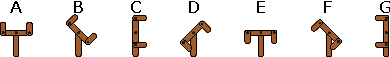
\includegraphics[width=0.7\textwidth]{lesson1/1-1_napoleon.pdf}
    \caption[Napoleon's semaphore]{Napoleon's semaphore encodings for the first five letters of the alphabet.}
    \label{fig:1-1_napoleon}
\end{figure}

Our last example of optical telegraphy is known as \textit{\textbf{Napoleon's semaphore}}.
This system was a lot more expressive than the signalling system of the Great Wall.
It worked on the basis of crane arms which could be arranged at certain angles.
An operator controlled levers and pulleys in order to arrange the arms at various angles. Each configuration of the arms carried its own meaning.
The arm configuration in Fig.~\ref{fig:1-1_napoleon} corresponds letter ``A".
Network of semaphores, each located around 10 kilometers apart, spanned all of France.
It was possible to send a message from Paris all the way to Venice, a distance of 1100 kilometers, in as little as few hours.
The record time of sending a message between Paris and Strasbourg in the east of France, is an astounding 1 hour.
This would be unthinkable by using the direct communication discussed above.

But as you can imagine there were some drawbacks of this method.
The biggest one being you had to have \textit{\textbf{direct visual contact}} with your neighboring semaphore.
Therefore the semaphore worked reliably only in good weather and during daytime.
On top of that, even though you could express an arbitrary message using this method, it was \textit{\textbf{physically demanding}} to operate the crane arms.

This brings us finally to the reason why Pony Express operated only for a single year.
It was due to the advent of \textit{\textbf{electrical telegraphy}} and the invention of the \textit{\textbf{Morse code}} that used electric signals to transmit messages.
It worked by encoding the letters of the alphabet into a series of ``dots'' and ``dashes'' as seen in Fig~\ref{fig:1-1_morse}.
An operator used a telegraph key to close an electric circuit to produce a signal of desired length.
Closing the electric circuit for a short time produced a ``dot'' while keeping the circuit closed for a longer time produced a ``dash''.
If the length of a ``dot'' is one unit, then a ``dash'' has length of 3 units.
Parts of the same letter are separated by 1 unit.
Different letters are separated by a space of 3 units while different words are separated by 7 units.
A skilled operator could transmit up to 30 words per minute, which were decoded by an operator at a distant telegraph station and passed onto the intended recipient.
This communication method allowed for messages to be delivered across length spanning continents within minutes, making direct communication such as Pony Express or optical telegraphy such as Napoleon's semaphore obsolete.

\begin{figure}[t]
    \centering
    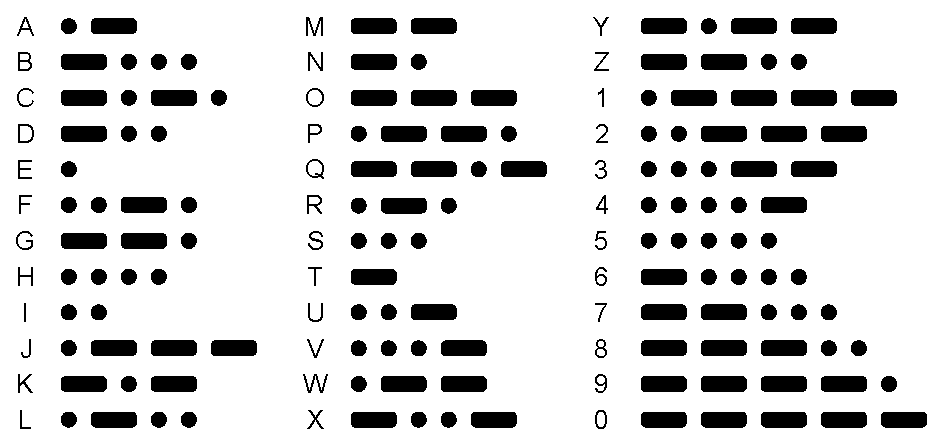
\includegraphics[width=0.8\textwidth]{lesson1/1-1_morse.eps}
    \caption[The Morse code]{The Morse code.}
    \label{fig:1-1_morse}
\end{figure}

Eventually, the electrical telegraph gave way to the \textit{\textbf{telephone}}, which implemented the dream of communication between humans and that was transmission of human voice.
Early telephone connections were simple point to point.
As the demand for communicating via the telephone grew, it became clear the \textit{\textbf{all-to-all}} approach would not work.
Imagine a network of $N$ telephones where all of them are directly connected to each other as seen in Fig.~\ref{fig:1-1_telephone}.
Consider adding a new telephone to the network.
In order for the new user to be able to call any of the existing telephones on the network, we have to add $N$ physical connections to all of the existing telephones.
Adding yet another telephone would require another $N+1$ connections.
The all-to-all approach is intuitive but simply does not \textit{\textbf{scale}} with the size of the network.

\begin{figure}[h]
    \centering
    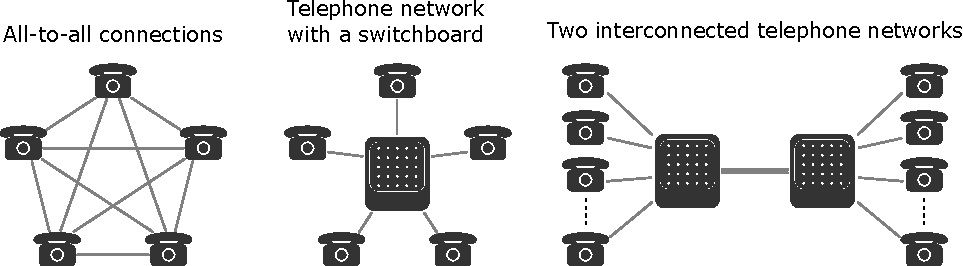
\includegraphics[width=\textwidth]{lesson1/1-1_rotary_telephone.pdf}
    \caption[Telephone networks]{Various topologies for telephone networks.}
    \label{fig:1-1_telephone}
\end{figure}

The solution came with the introduction of a \textit{\textbf{switchboard}}.
In order the call anybody on the network, each unit had to be connected only to the switchboard.
You first called the switchboard which would then connect you to the desired telephone unit.
With this approach, adding a new telephone to the network required to add a single connection to the switchboard, presenting a \textit{\textbf{constant scaling}}.
In other words, the effort of adding new users to the network did not increase with the size of the network.
Eventually, switchboards of different networks were interconnected together, allowing users from one network to call users on an entirely different network.

\begin{figure}[h]
    \centering
    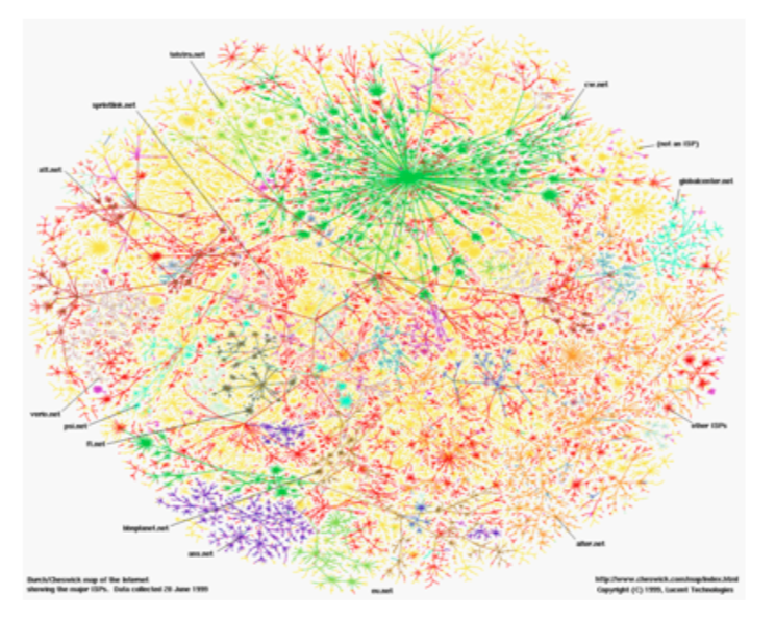
\includegraphics[width=0.8\textwidth]{lesson1/internetmap.eps}
    \caption[Map of the Internet.]{Map of the Internet.}
    \label{fig:1-1_internet}
\end{figure}

The Internet that our society has come to depend on so much works on the same principle.
It is not a single network but a \textit{\textbf{network of networks}}, allowing heterogeneous smaller networks to be interconnected.
Nowadays, a message sent from a laptop can be read by its recipient half-way around the world on their phone within seconds.
A broadcast stream of the FIFA World Cup Final can be enjoyed by millions around the world with minimal delay.
We can even start the air conditioning in some modern cars remotely without having to leave the comfort of our house.
Figure~\ref{fig:1-1_internet} depicts the closest thing to a ``map'' of the Internet that might be possible.
The dots do not represent individual hosts like computers of printers.
They represent entire networks!
The edges are the virtual connections between these networks.
The reason why this map of Internet is not accurate is due to its sheer size as well as as the fact that networks are constantly being added or removed.
Any ``map'' of the Internet that we might want to produce presents a monumental task, results of which would quickly be outdated.
The only purpose such a map would serve would be to make us realize how far humamity's ability to communicate has come and make us wonder what is the next step in evolution of communication.

% Today, we have the Internet which is a global spanning network of networks. Meaning that there are many different heterogeneous networks all connected to each other. So if you are using your phone, maybe you are connected to some telco tower which then relays the signal through the internet to wherever you wish. Also our computers are connected to modems via wi-fi, then these modems are connected to the Internet via ethernet cables. And basically everything is connected nowadays. We consume voice, and video entertainment, and news, and virtually we have access to any form of information that we wish to. And it's within a very short brief of time. So this image of internet is actually quite a simplification. In reality, what it looks like is more like this.

% So this rather confusing looking blob is a representation of the virtual connections between networks. So each of these little dots, they don't represent physical machines, they represent smaller networks. So you can see how complicated the routing in the Internet actually is. And this picture is about 20 years old. So nowadays probably it might look something a little bit even more impressive. So we have started with people gathering around campfires and sharing information, to having a truly global internet. But for us this is only where the journey begins. In this course, we will tell you what lies beyond the classical internet. What are the necessary tools to get there. And what are the challenges that face us.

\section{Analog to digital}

%Step 2: Analog to digital. 

The methods of communication described in the previous section were all very different from each other.
However, at a fundamental level they all followed the same basic principle depicted in Fig.~\ref{fig:1-2_communication}.
A sender \textit{\textbf{encodes}} her message into a form suitable for transmission.
The encoded message is then sent to the \textit{\textbf{decoder}}, which transforms the message back to a more easily readable form and passes it to the receiver.
To make this abstraction a little more concrete, let's consider the electrical telegraph as an example.
The sender brings her message to an operator who knows how to use the Morse key.
The operator uses the key to produce a series of dots and dashes, represented by short and long electrical signals which are transmitted to a distant telegraph station.
There, another operator receives these electrical signals, decodes them and produces the original message for to the receiver.

\begin{figure}[t]
    \centering
    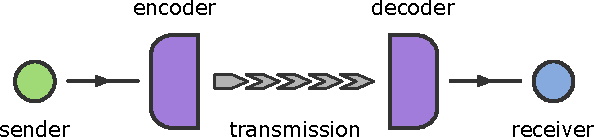
\includegraphics[width=0.7\textwidth]{lesson1/1-2_communication.pdf}
    \caption[Abstraction of communication]{Abstract representation of communication between a sender and a receiver.}
    \label{fig:1-2_communication}
\end{figure}

Immediate question that arises is what are some good ways of encoding the message.
The first method that we consider is encoding the message using an \textit{\textbf{analog}} signal.
Analog signals can admit a continuum of values.
We perceive the world around us as analog.
The loudness of sounds varies continuously from a quiet whisper to a loud music concert.
Temperature rises and falls in a continuous way as measured by our thermometers.
The three primary colors can be mixed together to produce a continuous spectrum of colors.
We have evolved to process these types of analog signals, therefore it makes sense to try and use analog signals to encode our messages.
The key is that analog signals can take on values from a continuous interval, representing the range of some quantity.
For example the voltage of an electric circuit can varied continuously depending on the pressure of sound waves in the microphone of a old telephone.
Early AM radio signals and old TV broadcasting used continuous sinusoidal waves that required simple technology to produce and decode.

\begin{figure}[t]
    \centering
    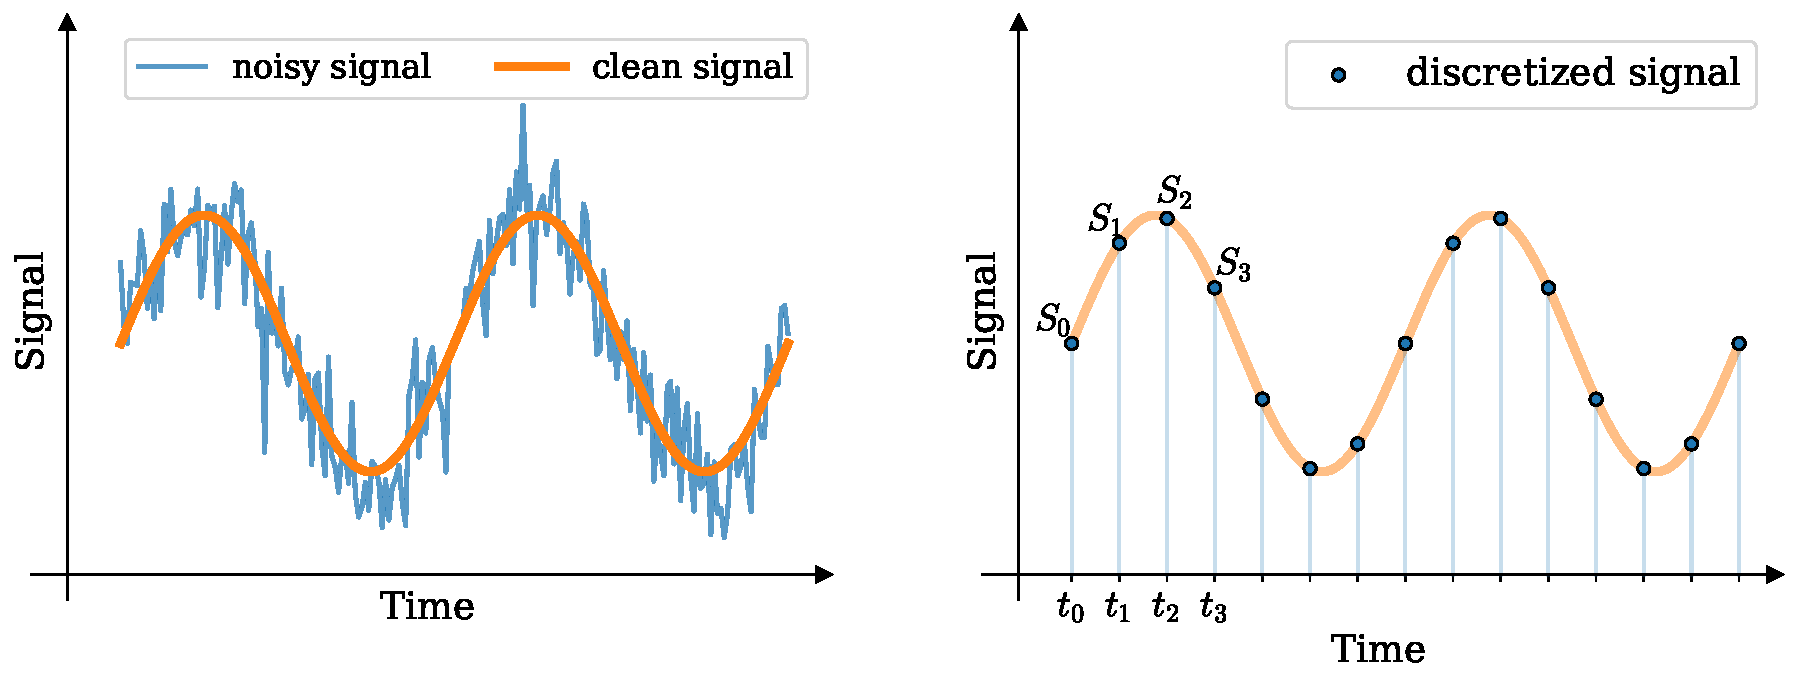
\includegraphics[width=\textwidth]{lesson1/1-2_signals.pdf}
    \caption[Continuous and discrete signals]{Analog signal subjected to noise on the left. The right figure shows how the analog signal can be discretized.}
    \label{fig:1-2_signals}
\end{figure}

One problem with analog signals is that they are \textit{\textbf{susceptible to noise}}.
Even small changes to the signal can alter the meaning of the transmitted message.
Due to this sensitivity to noise, analog signals are also difficult to copy.
Every time an analog signal gets copied, it degrades in quality due to both the noise as well as the finite accuracy the signal read out.

Figure~\ref{fig:1-2_signals} shows a clean analog sinusoidal signal in orange.
The blue jagged line represents the original signal affected by noise.
The noisy signal may have a meaning similar to the original noiseless message or may be quite different.

Alternative to analog signals is \textit{\textbf{digital}} signals.
Digital signals are very different from analog signals, they only use a discrete set of values to represent the message and encode it.
We can take the original analog signal, and try to encode it digitally.
A way to do it is to \textit{\textbf{sample}} the analog signal at discrete time steps $t_0$, $t_1$, $t_2$, $t_3$ and so on, as shown on the right side of Fig.~\ref{fig:1-2_signals}.
The encoded digital signal is now a set of discrete vales,
\begin{equation}
    S_0, S_1, S_2, S_3, \ldots,
\end{equation}
each of some finite accuracy.

The accuracy with which we can reproduce this analog signal depends how often we look and measure the signal, which is known as the \textit{\textbf{sampling rate}}.
For slowly varying signals, we don't have to sample that often, and we will still do a pretty good job of encoding the analog signal accurately.
But for analog signals that vary fast, we should sample also with higher frequency.
Digital signals are less affected by noise and are therefore easier to copy.
Other advantages include the ease of producing digital signals and ease of processing with digital logic.


\section{Bits as building blocks}

% Step three: Bits as building blocks. 

We have seen that digital signals can be more practical than analog signals when it comes to communication.
The question now is how do we represent these digital signals.
We saw an example of a digital system with the Napoleon's semaphore.
Let's go back to it and consider it again.
In order to send a message, for example ``WAR IS OVER'', the arms have to be rearranged as shown in Fig.~\ref{fig:1-3_warisover}.

\begin{figure}[t]
    \centering
    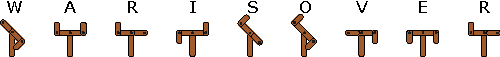
\includegraphics[width=0.8\textwidth]{lesson1/1-3_warisover.pdf}
    \caption[Message with Napoleon's semaphore]{Encoding a short message using Napoleon's semaphore.}
    \label{fig:1-3_warisover}
\end{figure}

What does it take to change the state of the semaphore?
Changing the state of the semaphore from ``A'' to ``R'' does not require that much effort.
All we have to do is change the state of one of the side arms and fold it onto the main arm.
On the other had, going from ``W'' to ``A'' requires changing the state of the main arm as well as the two side arms.
This change requires both physical effort as well as longer time.

\begin{figure}[t]
    \centering
    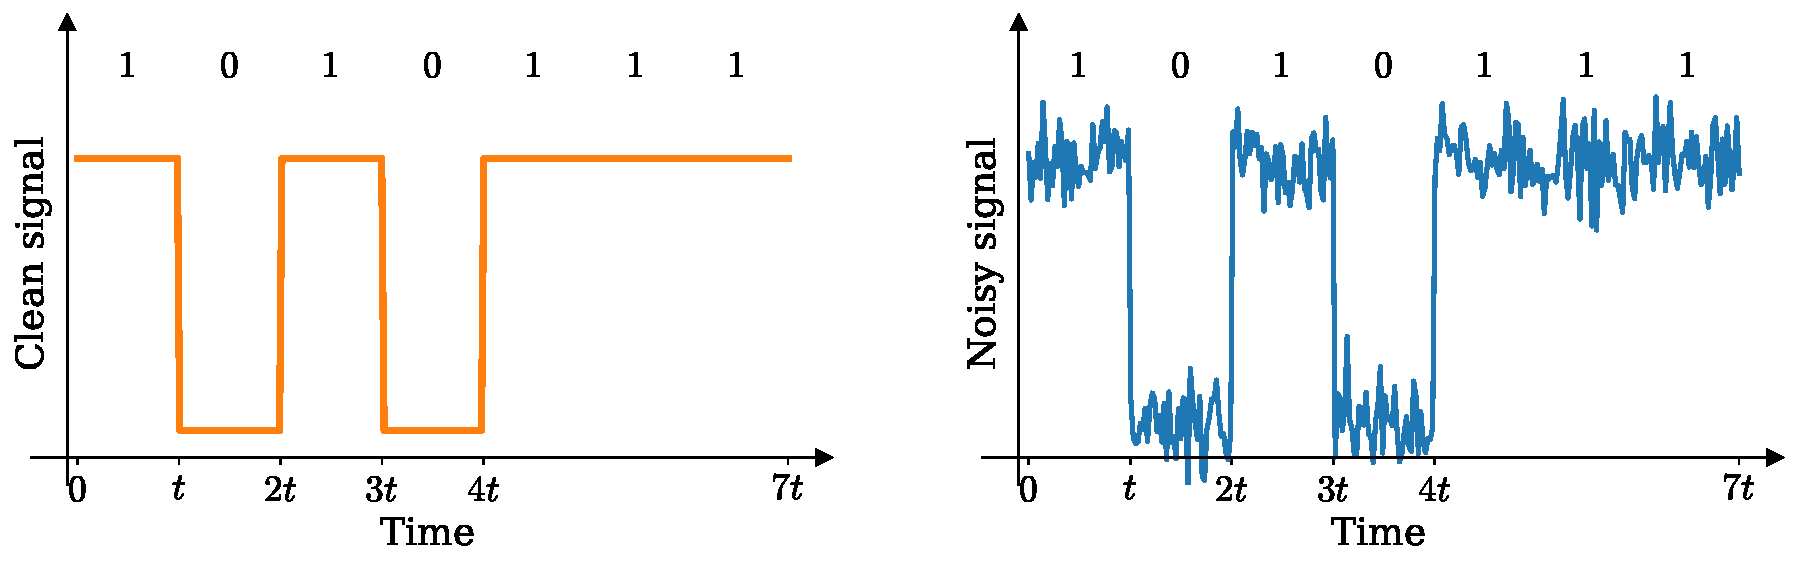
\includegraphics[width=\textwidth]{lesson1/1-3_morse_signal.pdf}
    \caption[Morse code signal]{Physical representation of the Morse code signal for the letter ``U''.}
    \label{fig:1-3_morse_signal}
\end{figure}

A good representation for digital signals should require as little effort and time as possible in order to change the state of the digital signal.
This suggests that having fewer internal states in order to produce a better encoding for the message.
The Morse code is such an example, where we only have two internal states.
The letter ``U'' is encoded by two dots followed by a dash.
The physical signal that represents this encoding is shown in Fig. \ref{fig:1-3_morse_signal} on the right.
The signal is switched on for a short time to represent a dot and for a long time to represent the dash.
It is the presence or absence of a signal that conveys the information.
Always, when you change from no signal to signal, or you know that the signal is constant, or it continues to be absent, then this carries a small amount of information.

This unit of information is known as a \textit{\textbf{bit}}, which is short for \textit{\textbf{binary digit}}.
In classical computation and in digital communication, it is the basic unit of information.
It conveys the message of something being true or false, the signal being on or off.
Usually we write the two states of a bit as 0 or 1.
The signal on the left of Fig.~\ref{fig:1-3_morse_signal} encoding the letter ``U'' in Morse code can be written using bits as 1010111, where zeros and ones denote the state of the bit at different times.
Right side of Fig.~\ref{fig:1-3_morse_signal} shows how the clean signal looks like when affected by noise.
The different states of the bit can still be easily distinguished from each other, hence the meaning of the message can be read out without any ambiguity.
Digital signals are generally more resilient to noise than analog signals.

We have said that a single bit can hold two different values.
How many different values can multiple bits, also called \textit{\textbf{bit strings}} hold?
The following table lists all possible bit string for 1, 2, 3, and 4 bits.
\begin{table}[h]
    \centering
    \begin{tabular}{c|c|c}
        Number of bits  & Possible bit strings & Total number \\
        \hline
        1 & 0, 1 & 2 \\
        2 & 00, 01, 10, 11 & 4 \\
        3 & 000, 001, 010, 011, 100, 101, 110, 111 & 8 \\
        4 & 0000, 0001, 0010, 0011, 0100, 0101, 0110, 0111 & 16 \\
        & 1000, 1001, 1010, 1011, 1100, 1101, 1110, 1111 & 
    \end{tabular}
\end{table}
It is clear that the total number of possible bit string values for $N$ bits is $2^N$.

Bits can be used to encode decimal numbers.
Let's examine how decimal notation works first.
The decimal system uses ten numerals; 0-9.
In a decimal number, the rightmost digit represents ones, the next digit to the left represents tens, the next hundreds and so on.
For example, the number 1024 can be written in terms if powers of ten as follows,
\begin{equation}
    1024 = 1 * 10^3 + 0 * 10^2 + 2 * 10^1 + 4 * 10^0.
\end{equation}
This idea carries over to binary numbers where the digits can only take values of 0 or 1, and represent multiples of powers of two.
Let7s see how we can write the binary number 1001 in decimal notation,
\begin{equation}
    1001 = 1 * 2^3 + 0 * 2^2 + 0 * 2^1 + 1 * 2^0 = 9.
\end{equation}

Bits are the building blocks of modern communication.
They are robust to noise, can be easily used to encode and decode information, and modern computers are very good at processing them.
Given that bits admit only two values, we might easily consider them to be the most fundamental units of information.
In these lectures, we will learn that this is not quite true.
We will see that quantum communication relies on more fundamental units of information.
Classical bits are merely special cases of their quantum cousins.


\section{Quantum communication}

Information is physical.
It is carried by physical systems and it is the laws of physics that determine how we can process or communicate this information.
If we are only considering information processing in the context of classical mechanics, classical electromagnetism, and classical optics, then this will give us tools and ways of processing and communicating the information classically.
However, if we expand our toolbox to include also quantum mechanics and quantum optics, then we are also expanding the ways in which we can process and communicate this information.

The question that we should answer before we start learning about quantum communication is, why do we need quantum mechanics?
Why do we want to use quantum mechanics to process and communicate information? Firstly, quantum mechanics is the fundamental theory of nature, currently as we understand it.
It describes the microscopic world where classical mechanics does not apply.
It makes some stunning predictions, which, however despite their counter-intuitiveness, have been tested very thoroughly over many decades.
So far, the theory has always been proven correct.
Furthermore, considering new laws of physics, and applying them to information processing and communication, often leads to new ways of processing and communicating this information.

These reasons in themselves are very fundamental, but there are also practical reasons.
The current computing technology is hitting a classical to quantum boundary.
Maybe you have heard of the Moore's law, which despite its name is an observation rather than a physical law.
Moore's Law states that the number of transistors on in an integrated circuit doubles about every two years.
It is astonishing that this observation has held for decades.
Chip manufactures have been able to pack orders of magnitudes more transistors onto The chips themselves are not getting any bigger, so in order for Moore's Law to hold is for the transistors to get smaller and smaller.
In the beginning, the transistors were approximately 10 microns across.
In the 1990s, they moved to about 600 nanometers.
And now we are at the level of single nanometers.
The transistors have got so small that they need to worry about the effects quantum mechanics have on the transistors' operation.

\begin{figure}[t]
    \centering
    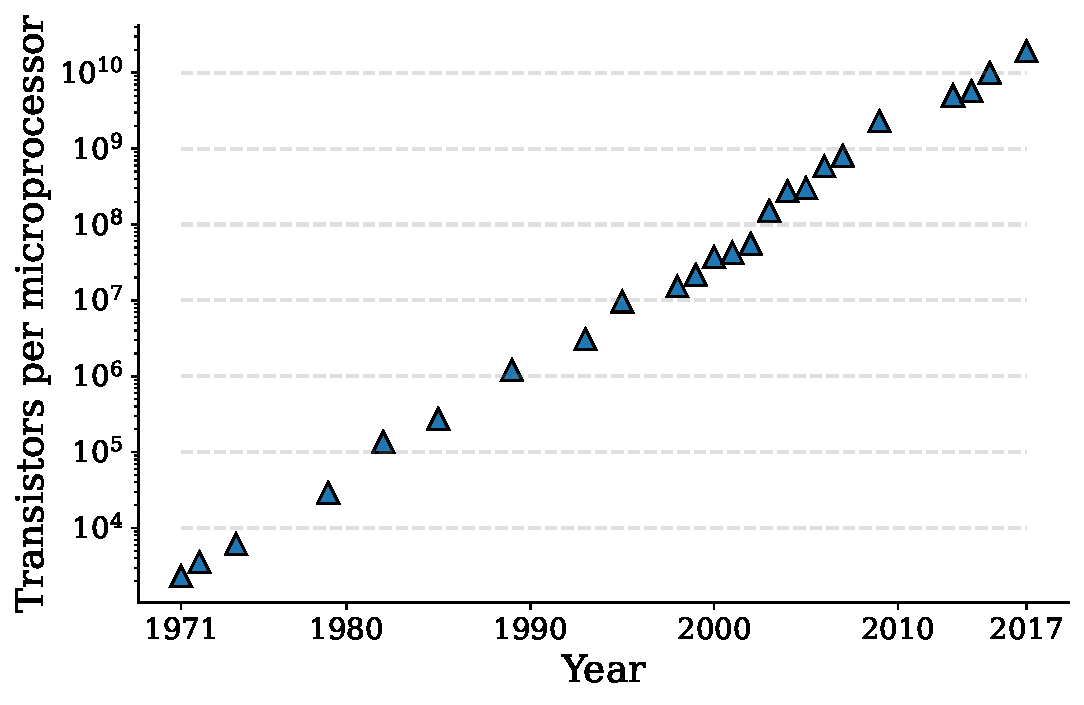
\includegraphics[width=0.8\textwidth]{lesson1/1-4_transistors.pdf}
    \caption[Moore's law.]{Number of transistors on a microprocessor has been doubling nearly every two years.}
    \label{fig:1-4_transistors}
\end{figure}

What are the two main ingredients that set quantum communication apart from its classical counterpart?
The first one is the \textit{\textbf{superposition principle}}.
This principle is not really anything new as it is observed in the classical world as well.
We are all familiar with superposition of waves.
What is meant by superposition principle in quantum communication is the ability of quantum bits to be in a superposition of their usual classical states.
The possibility of a quantum bit to be both on and off at the same time is mind-bending but is at the heart of quantum communication.

Expand the principle of superposition to multiple particles, we arrive at the concept of \textit{\textbf{entanglement}}.
Entanglement has no classical counterpart whatsoever.
It correlates distant quantum objects across large distances of space much more strongly than is possible using classical laws of nature.
The beauty of entanglement is that it allows for radically new ways to communicate and is used as a resource in quantum communication.
Distribution of entanglement is therefore one of the main jobs of quantum networks.

Is quantum communication difficult?
Quantum communication protocols are currently very difficult to implement.
Quantum systems are very delicate as they decohere extremely rapidly leading to loss of their quantum properties.
They go from being true and false at the same time, to being only true or only false.
Basically, they just become classical bits.

Quantum systems are difficult to build at the hardware level, but at the same time, it is also conceptually challenging to think about new ways of exploiting their quantum properties.
Designing new protocols for processing and communication in the quantum realm requires new tools.
It requires a completely new mental framework for how we approach problems, and how we solve problems.
This all seems very daunting but these challenges should be viewed as opportunities.
Quantum computation and quantum communication are vibrant and cross-disciplinary fields.
Engineers, physicists, mathematicians, and computer scientists are all working together on cracking difficult questions whose solutions will lead to incredible new quantum technologies.

\section{Security in the quantum age}

Quantum technologies carry the potential to impact a number of important areas.
Quantum simulation and computation is thought to bring about new methods in developing materials with novel and useful properties, as well as novel drugs.
Quantum metrology allows for measurements with unprecedented resolution and sensitivity.
Quantum machine learning aims to exploit the properties of quantum mechanics to enhance artificial intelligence.
Lastly, you may have heard that quantum computers will be able to crack some encryption schemes deployed currently.
This sounds like a doomsday scenario.
Since these lecture notes focus on quantum communication, we will briefly discuss what this claim means and show how quantum technologies can also enhance security.

\begin{figure}[t]
    \centering
    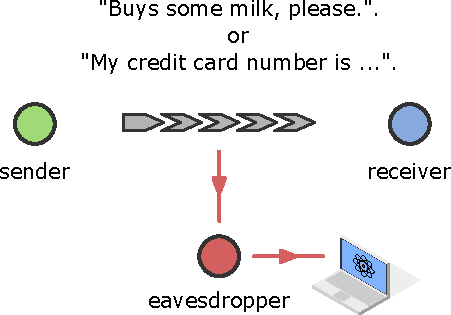
\includegraphics[width=0.5\textwidth]{lesson1/1-5_security.pdf}
    \caption[Security in the quantum age.]{An eavesdropper is trying to intercept and decrypt the message sent from the sender to the receiver.}
    \label{fig:1-5_security}
\end{figure}

Let's consider a sender wishing to send a message to a receiver as pictured in Fig.~\ref{fig:1-5_security}.
The message might be something mundane such as ``Buy some milk, please'' or might be something sensitive such as ``My credit card number is ...''.
Either way, messages sent over public channels are encrypted to preserve the privacy of the conversation between the sender and the receiver.
Let's consider a third party, an eavesdropper, who is trying to listen in on the conversation by intercepting the message.
Current classical encryption techniques offer \textit{\textbf{computational security}}, meaning that cracking them is not impossible, merely very difficult and would require enormous classical resources to do so.
Quantum algorithms exist that break this encryption.
An eavesdropper with access to a quantum computer could in principle intercept the encrypted message, use its quantum computer to break the code and listen in on the conversation with impunity.

To overcome this problem, the communicating parties need to resort to using \textit{\textbf{quantum key distribution}} (QKD).
With the help of the superposition principle or entanglement, the sender and the receiver can discover the eavesdropper's attempts to intercept and tamper with their messages.
They can then simply not transmit their sensitive message.
This method of encryption offers \textit{\textbf{information-theoretic security}}.
Such security does not rely on the computational difficulty of certain mathematical problems and therefore is more strong than computational security used currently.
For this reason, QKD is one of the primary applications of quantum networks.
We will explore the basics of QKD later in these lectures.

\section{Module Overview}
\label{sec:mod-over}

Before concluding the first chapter, let's have a brief look at the structure of this module.
The next three chapters deal with the basics of quantum mechanics relevant to quantum communication.
We will learn about quantum bits and how they are different from classical bits, consider how noise affects the state of quantum states and how we can describe this effect mathematically.
Finally, we will look at systems of multiple quantum bits.

Chapters 5-7 deal with basics of optics.
Light is an excellent information carrier and we will learn how lasers produce light.
We will discuss interference, one of the fundamental phenomena in both classical as well as quantum physics.
We will conclude this block of chapters by learning about waveguides and how light is guided in a network.

Chapters 8-10 look at fundamental quantum communication protocols.
We will learn how teleportation can be used to transmit information without sending the physical system encoding this information as well as how quantum key distribution works.

In chapters 11-13, we will look at the basics of quantum repeaters, a quantum technology that makes long-distance quantum communication possible.
The last two chapters look at quantum repeater systems.

There are some basic prerequisites for this module such as linear algebra (meaning vector and matrix multiplication; eigenvectors and eigenvalues; also, we will use the tensor product which will be introduced in this book), discrete probability, and complex numbers (e.g., $i = \sqrt{-1}$ and Euler's equation, $e^{i\pi} + 1 = 0$). It's very helpful if you have some introduction to quantum computing, and programming and classical computing, and if you know a little bit about computer networks that's very helpful as well.
Other than that there are no physics requirements.

If you don't have some of this background yet, there are a lot of online materials, particularly our MOOC (massively open online course), "Understanding Quantum Computers", which is targeted at learners at the high school level and requires very minimal math.
On top of that it's available in English, Japanese, Thai and Indonesian.
If you would like to learn a little bit more about some basic linear algebra you can have a look at the playlist on Professor Van Meter's YouTube channel, or there are many other courses available. Other modules from the Quantum Academy of Science and Technology (supported by the Q-Leap Education office in Japan), cover some of this background material as well, and may be available to you.


% \begin{figure}[H]
%     \centering
%     \includegraphics[width=0.9\textwidth]{lesson1/communication.eps}
%     \label{fig:1-1}
%     \caption{Evolution of communication.}
% \end{figure}

% insert photo here
% \begin{figure}[H]
%     \centering
%     
\includegraphics[width=0.6\textwidth]{lesson1/ponyexpress.eps}
%     \label{fig:1-2}
%     %\justification=<centering>
%     \caption{Pony Express.}
% \end{figure}

% insert photo here
% \begin{figure}[H]
%     \centering
%     
\includegraphics[width=0.9\textwidth]{lesson1/万里の長城.eps}
%     \label{fig:1-3}
%     \caption{The Great Wall of China.}
% \end{figure}

% Insert photo here
% \begin{figure}[H]
%     \centering
%     \includegraphics[width=0.9\textwidth]{lesson1/napoleon.eps}
%     \label{fig:1-4}
%     \caption{Napoleon's semaphore.}
% \end{figure}

% insert photo here. TODO: How to make these side-by-side?
% \begin{figure}[H]
%     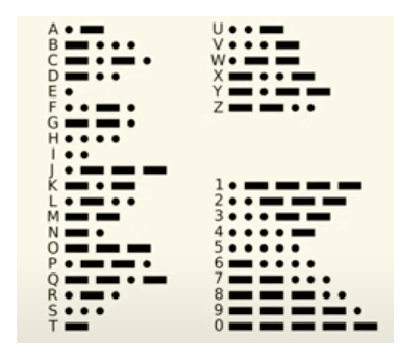
\includegraphics[width=0.3\textwidth]{lesson1/morse.eps}
%     \label{fig:1-5}
%     \caption{Morse signal.}
% \end{figure}
% \begin{figure}[H]
%     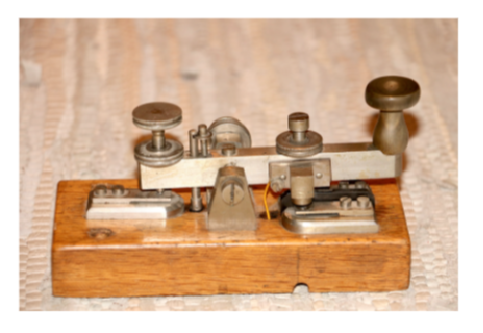
\includegraphics[width=0.3\textwidth]{lesson1/morsekey.eps}
%     \label{fig:1-6}
%     \caption{Morse key.}
% \end{figure}
% \iffalse
% \begin{figure}
%     \centering
%     \begin{minipage}{0.45\textwidth}
%         \centering
%         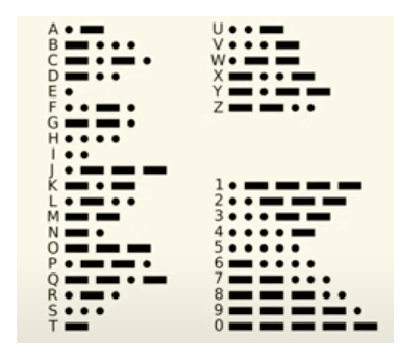
\includegraphics[width=0.9\textwidth]{lesson1/morse.eps} % first figure itself
%         \caption{first figure}
%     \end{minipage}\hfill
%     \begin{minipage}{0.45\textwidth}
%         \centering
%         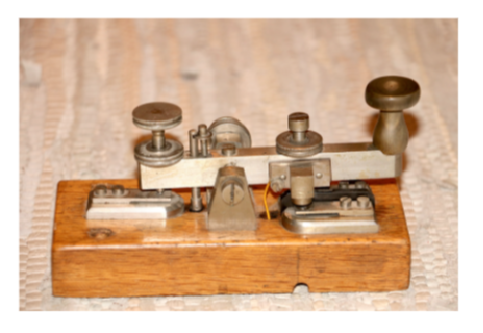
\includegraphics[width=0.9\textwidth]{lesson1/morsekey.eps} % second figure itself
%         \caption{second figure}
%     \end{minipage}
% \end{figure}
% \fi

% Insert point-to-point pic here
% \begin{figure}[H]
%     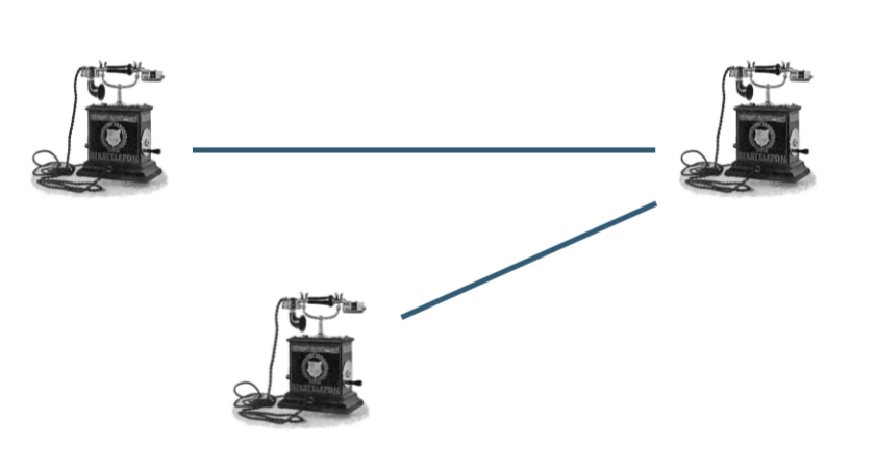
\includegraphics[width=0.8\textwidth]{lesson1/pointpoint.eps}
%     \label{fig:1-7}
%     \caption{Point-to-point.}
% \end{figure}

% Insert switchboard pic here.
% \begin{figure}[H]
%     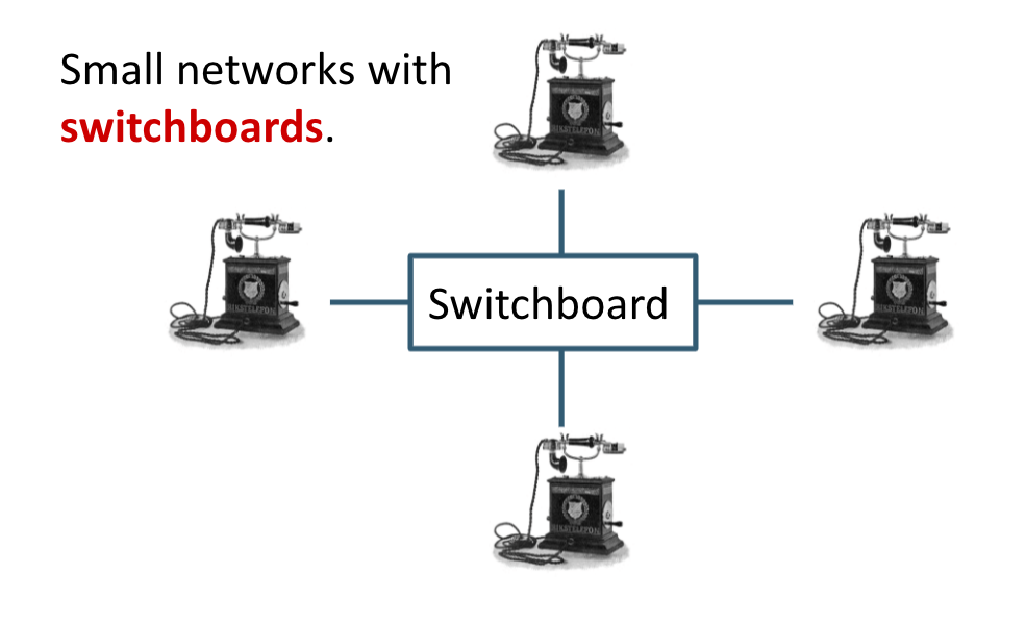
\includegraphics[width=0.8\textwidth]{lesson1/switchboard.eps}
%     \label{fig:1-8}
%     \caption{Switchboard.}
% \end{figure}
% insert internet pic here
% \begin{figure}[H]
%     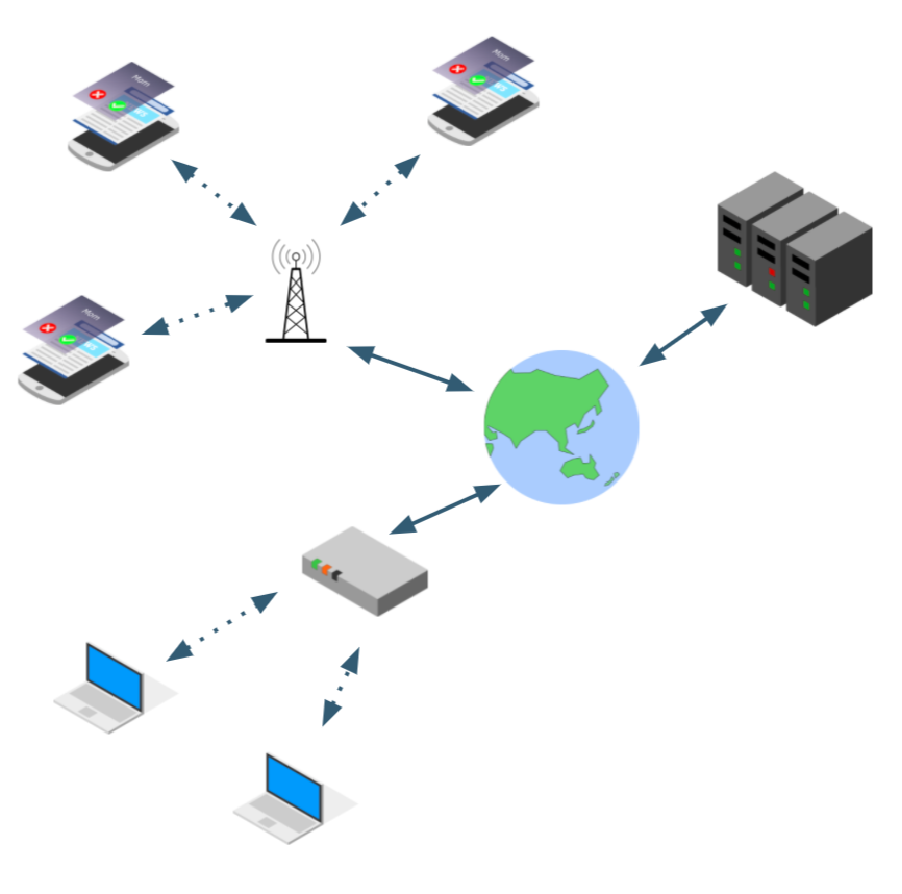
\includegraphics[width=0.8\textwidth]{lesson1/internet.eps}
%     \label{fig:1-9}
%     \caption{The Internet.}
% \end{figure}
% insert picture here
% \begin{figure}[H]
%     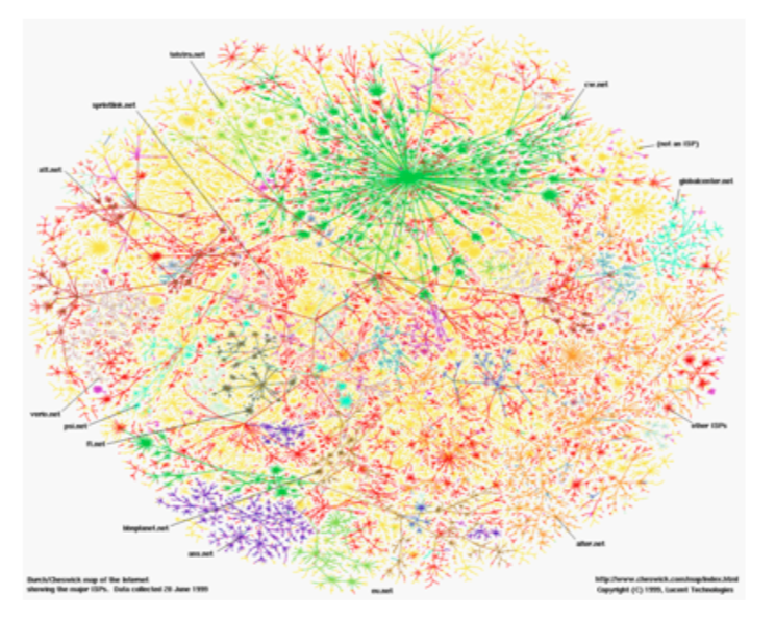
\includegraphics[width=0.8\textwidth]{lesson1/internetmap.eps}
%     \label{fig:1-10}
%     \caption{Network of networks.}
% \end{figure}

% \begin{figure}[H]
%     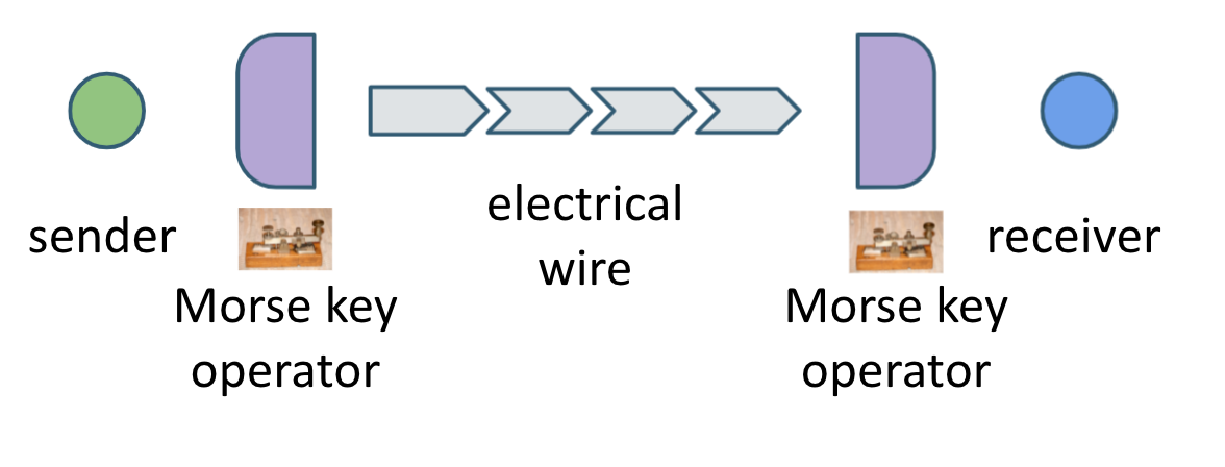
\includegraphics[width=0.8\textwidth]{lesson1/sender_receiver.eps}
%     \label{fig:1-11}
%     \caption{Sender and receiver.}
% \end{figure}


% insert continuous signal picture.
% \begin{figure}[H]
%     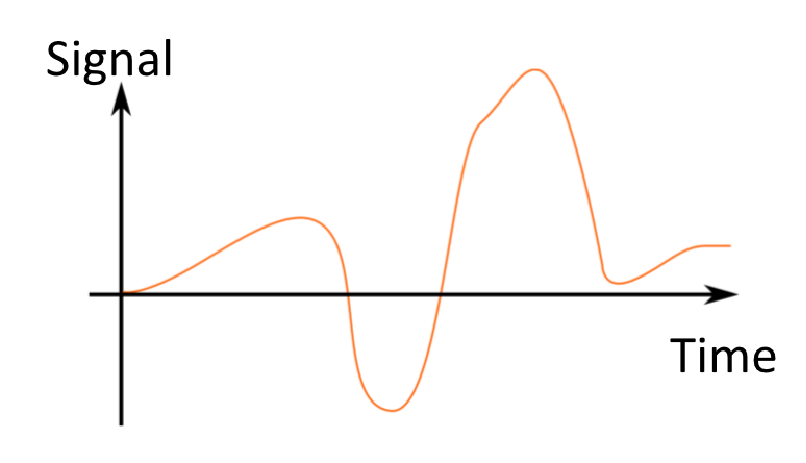
\includegraphics[width=0.8\textwidth]{lesson1/continuoussignal.eps}
%     \label{fig:1-12}
%     \caption{Analog communication}
% \end{figure}

% insert continuous signal w/ disruptive noise included here. 
% \begin{figure}[H]
%     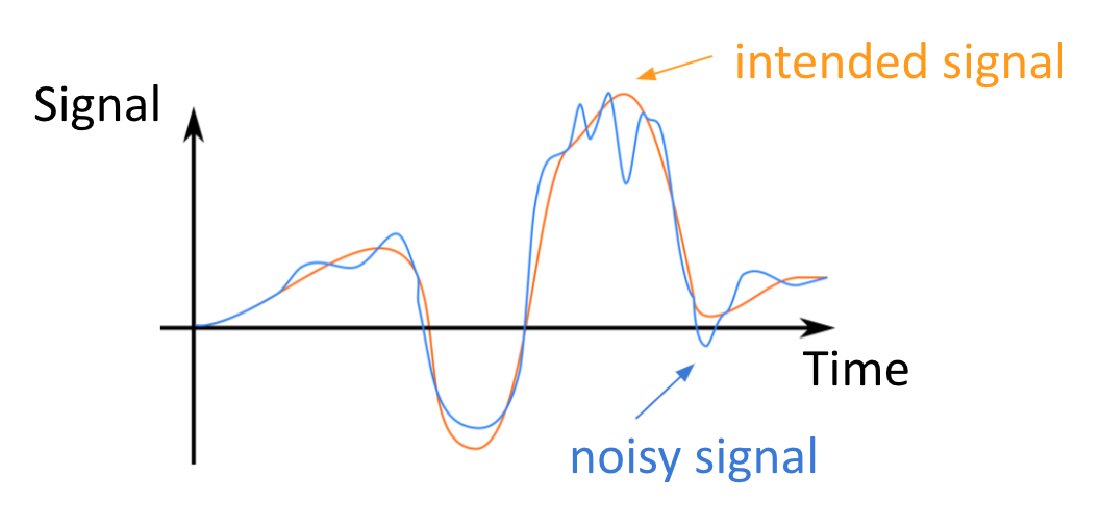
\includegraphics[width=0.8\textwidth]{lesson1/continuous_signal_noise.eps}
%     \label{fig:1-13}
%     \caption{Analog signal and noise.}
% \end{figure}

% Insert discrete digital signal pic  w/ t_0, t_1, t_2 here
% \begin{figure}[H]
%     \centering
%     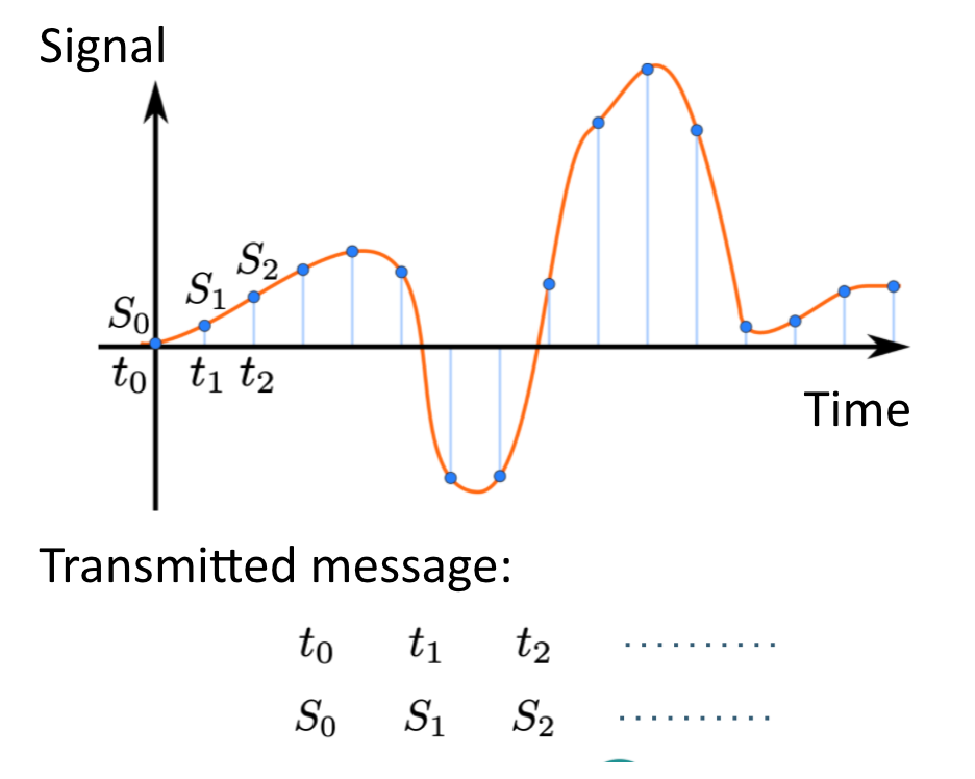
\includegraphics[width=0.8\textwidth]{lesson1/discre_signal.eps}
%     \label{fig:1-14}
%     \begin{center}
%         \caption{Discrete signals.}
%     \end{center}
% \end{figure}

% insert war is over
% \begin{figure}[H]
%     \centering
%     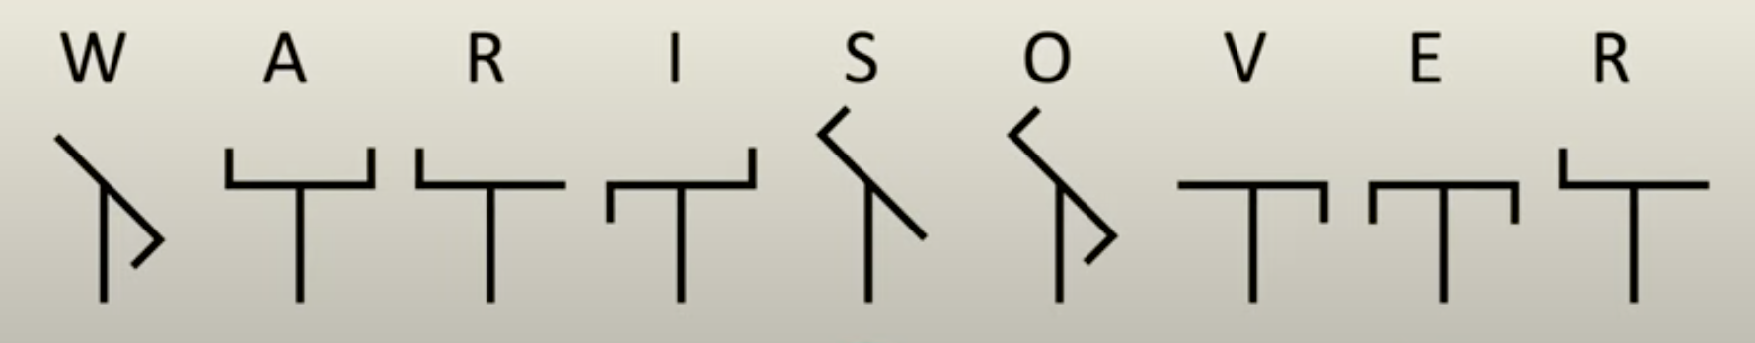
\includegraphics[width=0.5\textwidth]{lesson1/warisover.pdf}
%     \label{fig:1-15}
%     \begin{center}
%         \caption{Letters spelling "War is over".}
%     \end{center}
% \end{figure}

% Insert A -> R, W -> 10 
% \begin{figure}[H]
%     \centering
%     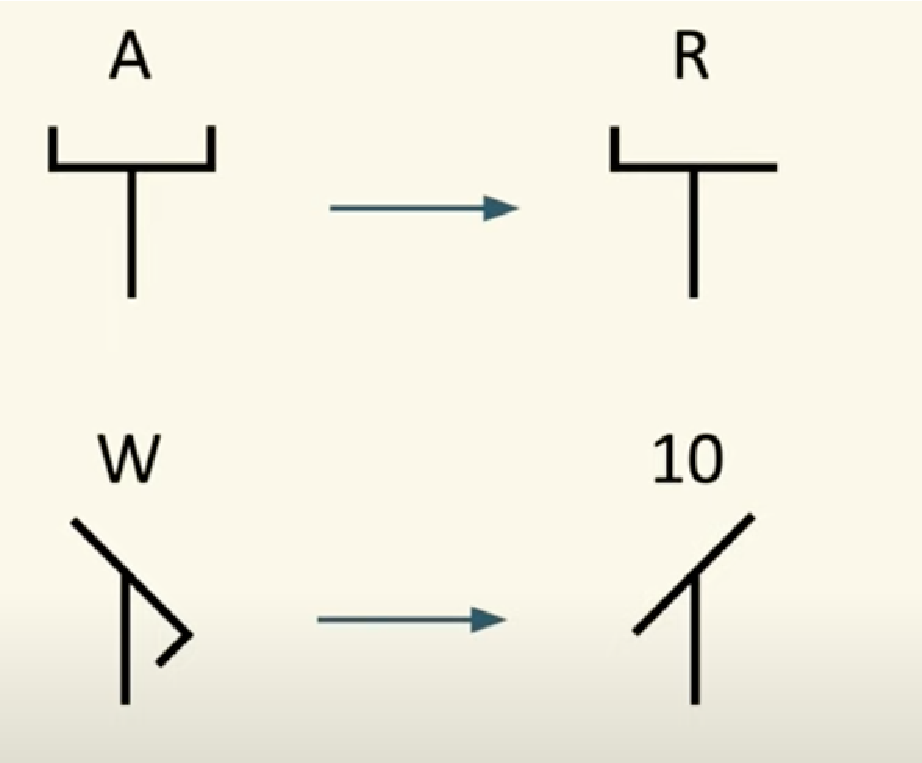
\includegraphics[width=0.8\textwidth]{lesson1/a_to_r.pdf}
%     \label{fig:1-16}
%     \begin{center}
%         \caption{Letters.}
%     \end{center}
% \end{figure}

% Insert U encoding
% \begin{figure}[H]
%     \centering
%     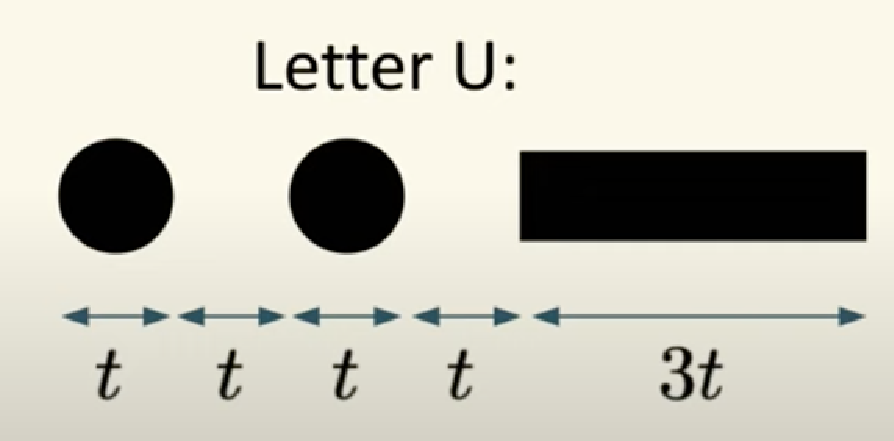
\includegraphics[width=0.8\textwidth]{lesson1/letter_u.pdf}
%     \label{fig:1-17}
%     \begin{center}
%         \caption{Morse code letter U.}
%     \end{center}
% \end{figure}

% insert morse graph
% \begin{figure}[H]
%     \centering
%     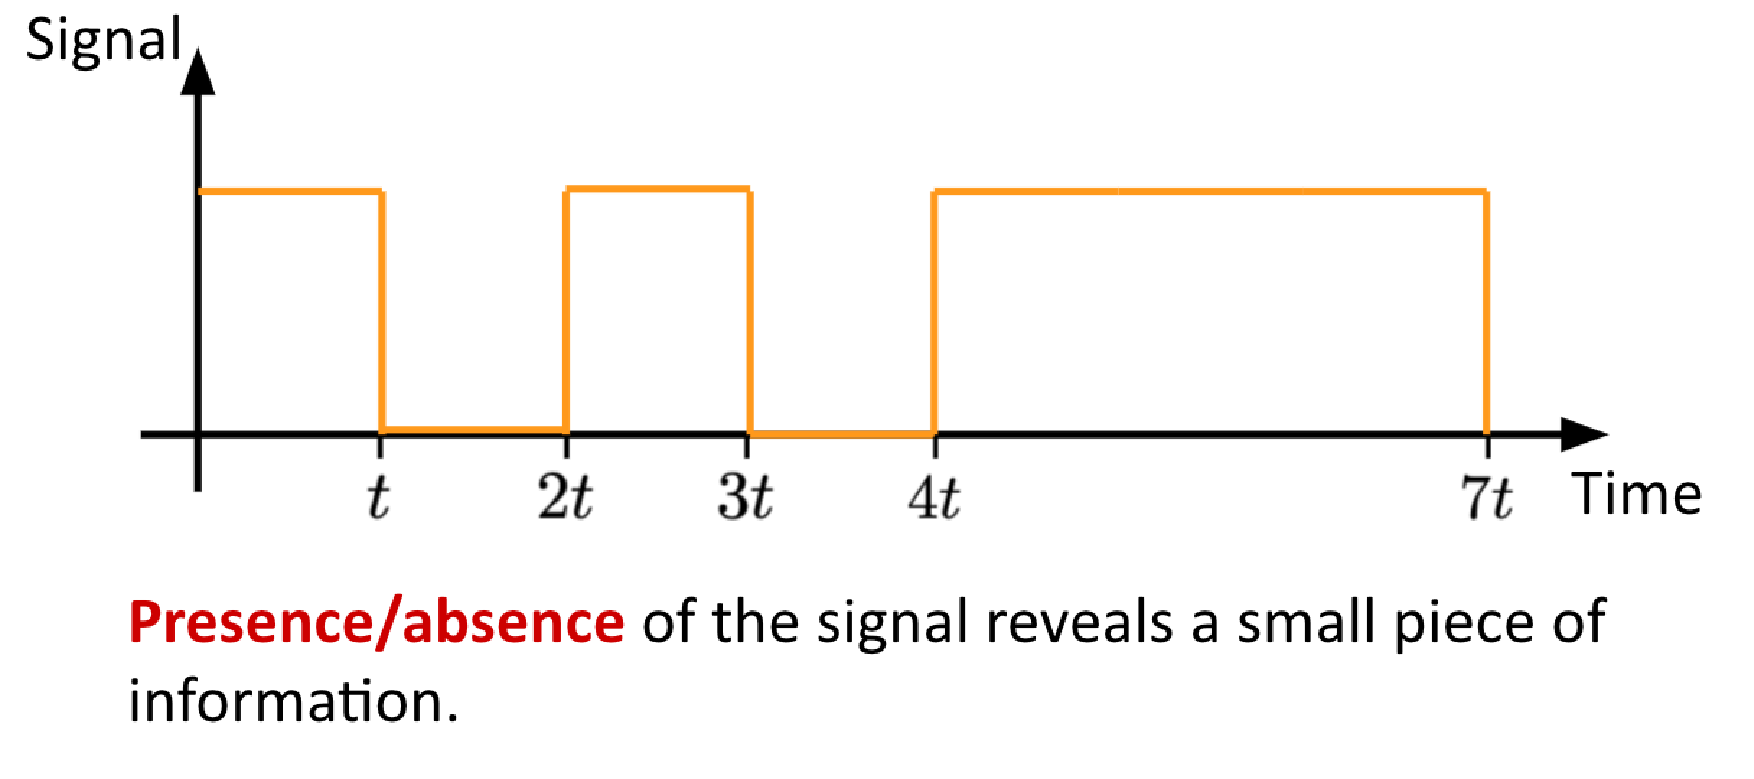
\includegraphics[width=0.8\textwidth]{lesson1/presence_abscence.pdf}
%     \label{fig:1-18}
%     \begin{center}
%         \caption{Morse code.}
%     \end{center}
% \end{figure}

% \begin{figure}[H]
%     \centering
%     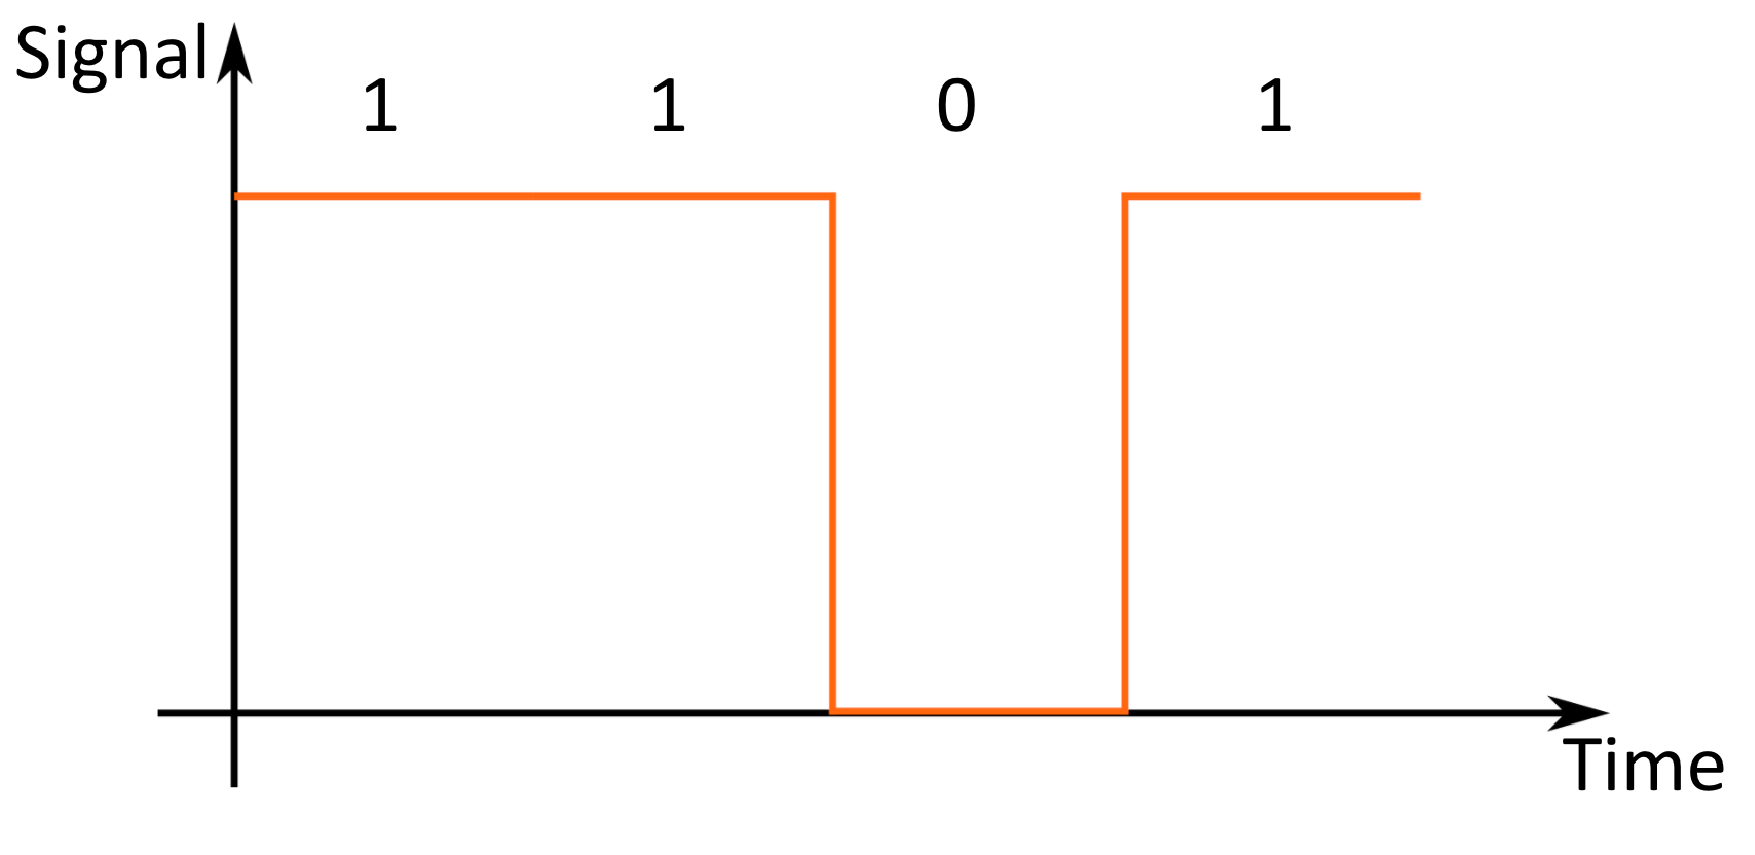
\includegraphics[width=0.8\textwidth]{lesson1/presence_abscence_bit.pdf}
%     \label{fig:1-19}
%     \begin{center}
%         \caption{Bits.}
%     \end{center}
% \end{figure}
% insert graph w/ noise
% \begin{figure}[H]
%     \centering
%     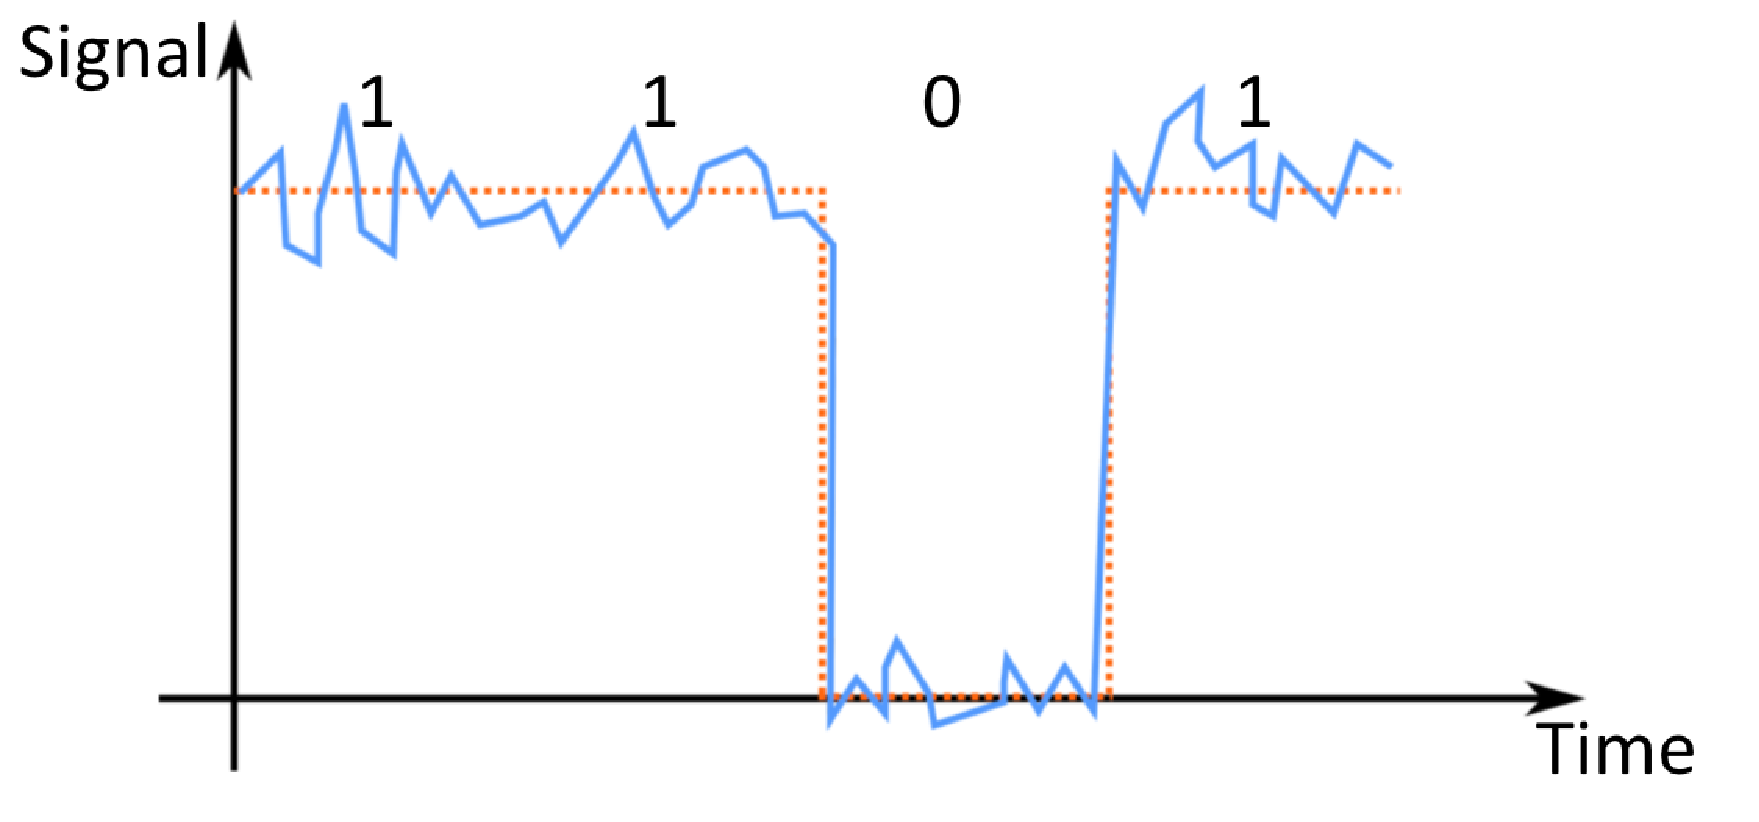
\includegraphics[width=0.8\textwidth]{lesson1/presence_abscence_noise.pdf}
%     \label{fig:1-20}
%     \begin{center}
%         \caption{Presence or absence as a bit.}
%     \end{center}
% \end{figure}

% insert bit permutations slide
% \begin{figure}[H]
%     \centering
%     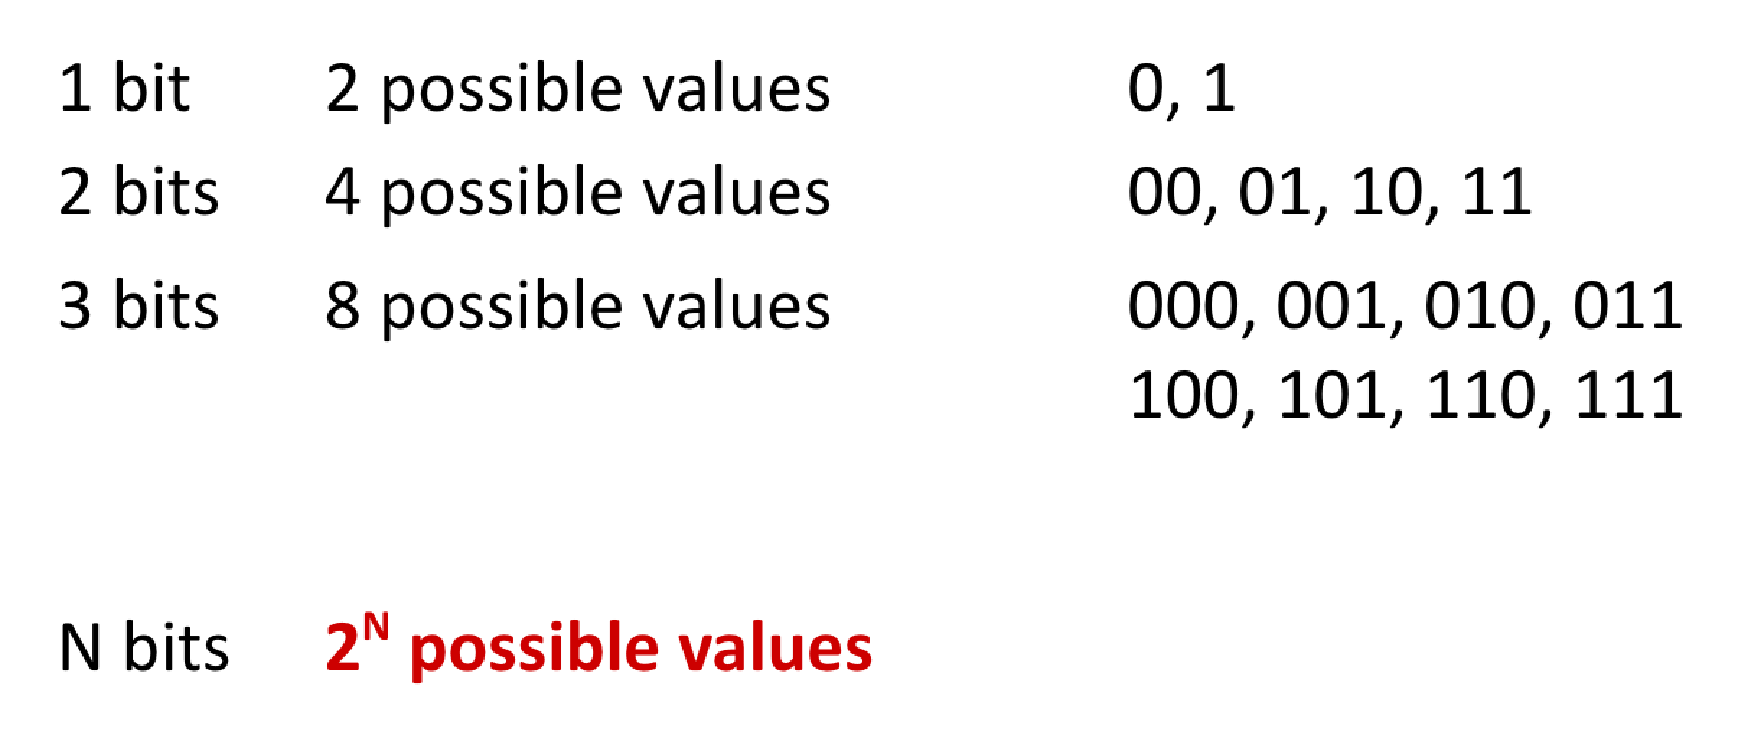
\includegraphics[width=0.8\textwidth]{lesson1/binary_notation.pdf}
%     \label{fig:1-21}
%     \begin{center}
%         \caption{Binary notation.}
%     \end{center}
% \end{figure}

% insert decimal notation
% \begin{figure}[H]
%     \centering
%     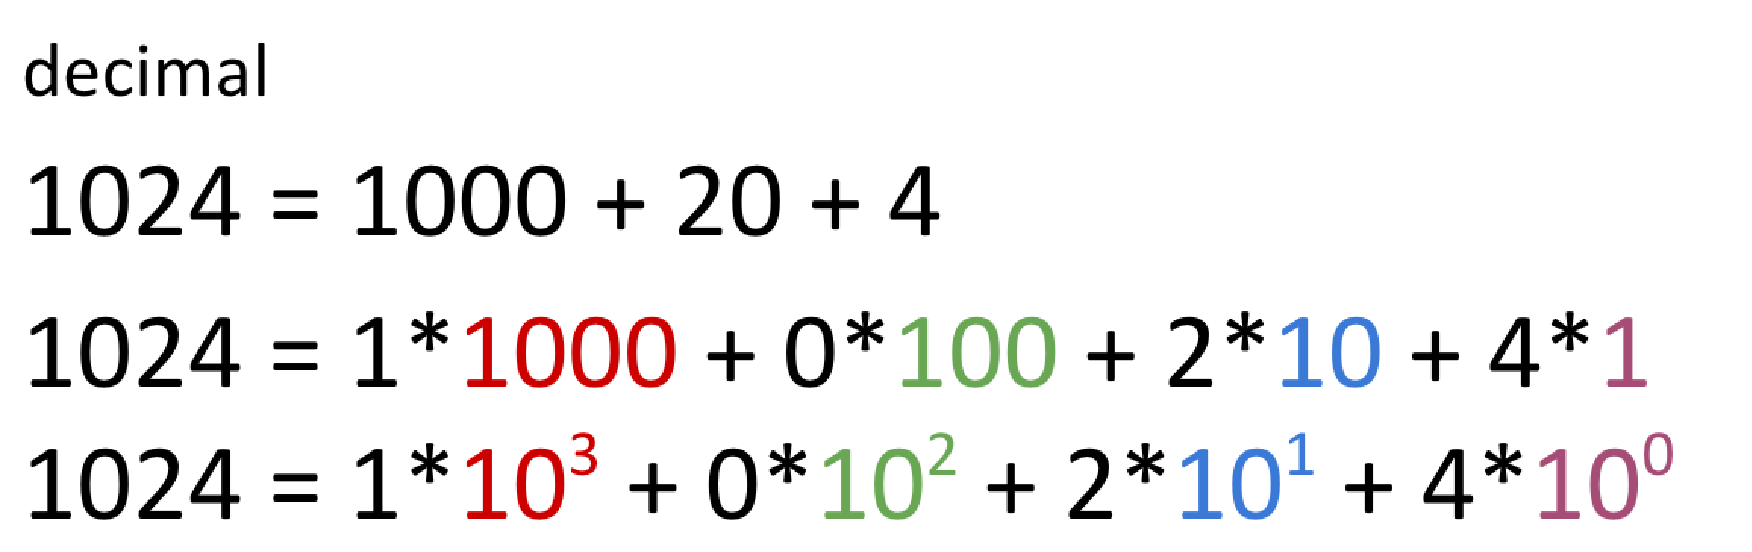
\includegraphics[width=0.8\textwidth]{lesson1/decimal_notation.pdf}
%     \label{fig:1-22}
%     \begin{center}
%         \caption{Decimal notation.}
%     \end{center}
% \end{figure}

% insert binary notation
% \begin{figure}[H]
%     \centering
%     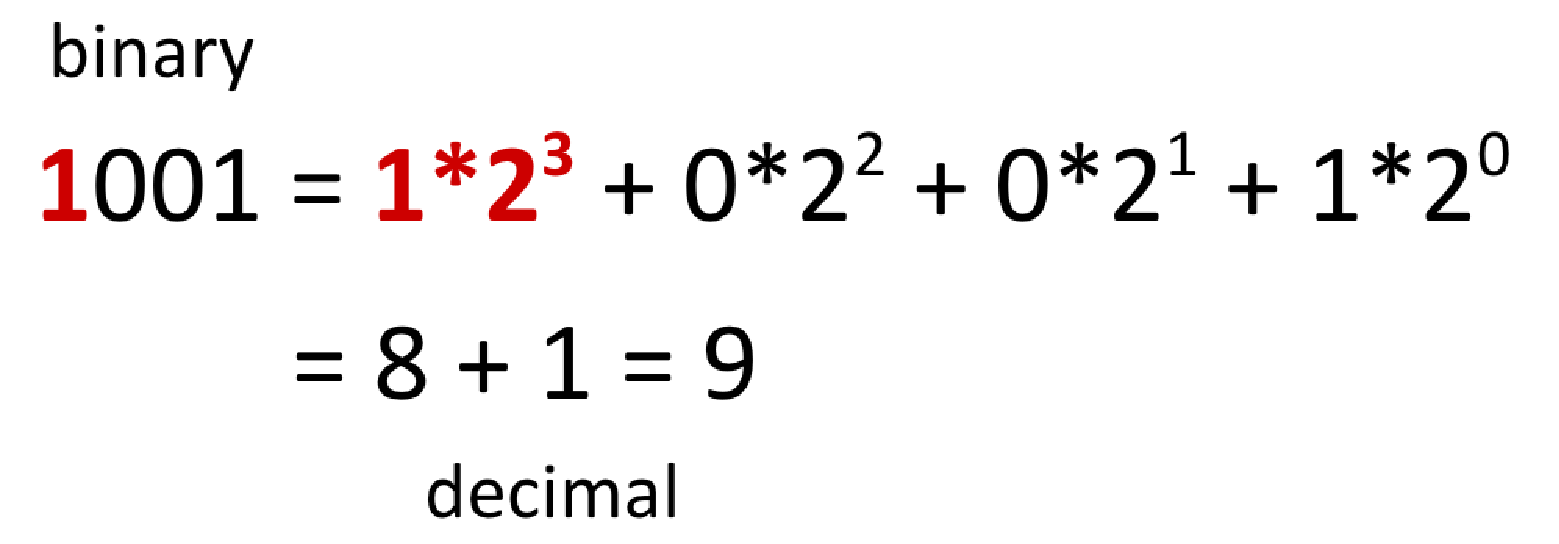
\includegraphics[width=0.8\textwidth]{lesson1/binary_ex.pdf}
%     \label{fig:1-23}
%     \begin{center}
%         \caption{Binary notation.}
%     \end{center}
% \end{figure}

% Insert classical VS quantum slide
% \begin{figure}[H]
%     \centering
%     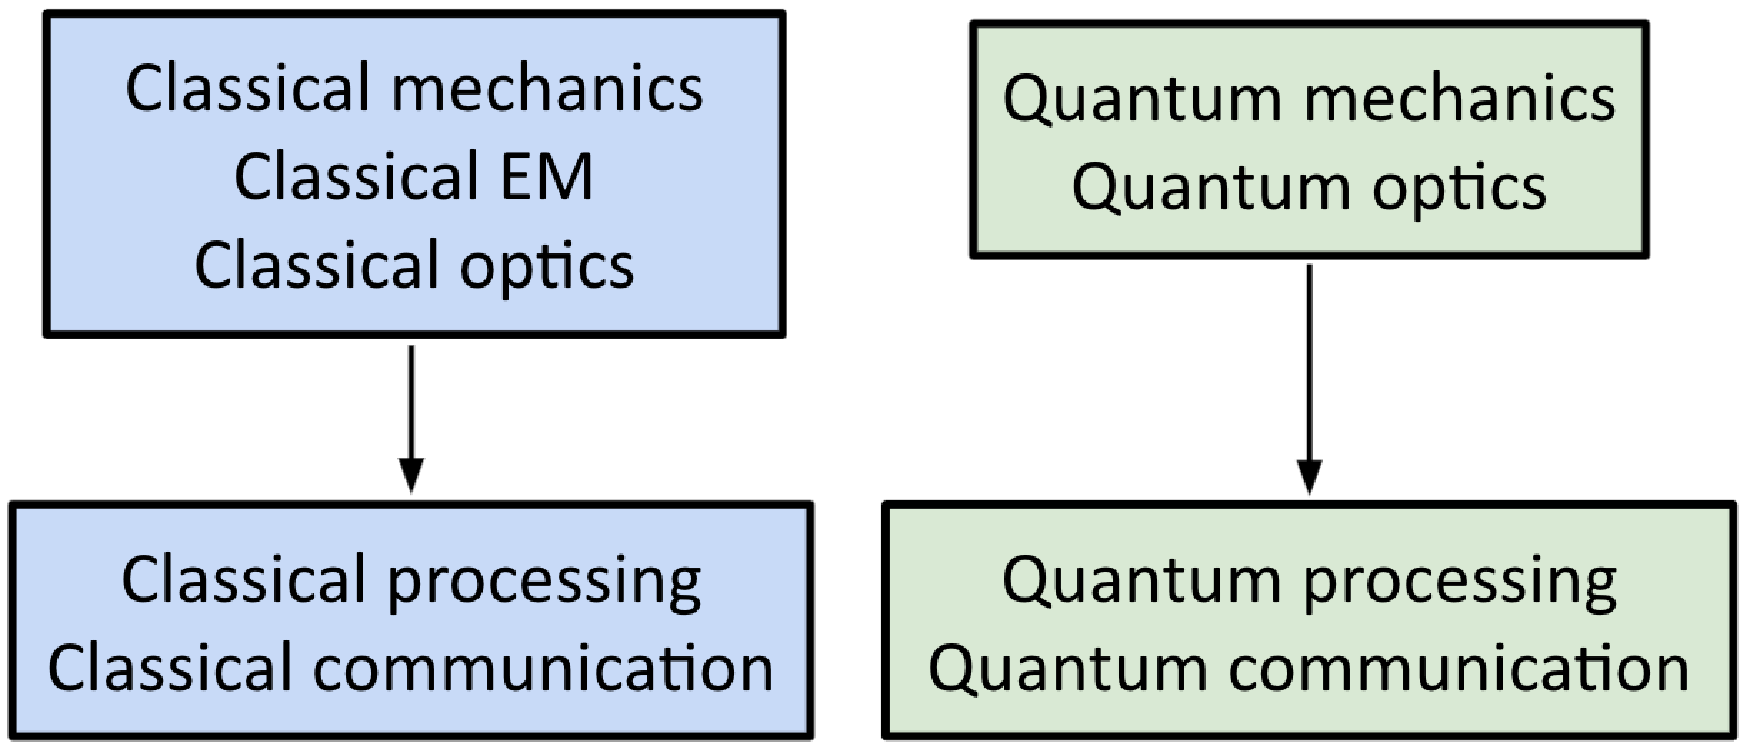
\includegraphics[width=0.8\textwidth]{lesson1/comparsion.pdf}
%     \label{fig:1-24}
%     \begin{center}
%         \caption{Classical and quantum.}
%     \end{center}
% \end{figure}

% Moore's law graph
% \begin{figure}[H]
%     \centering
%     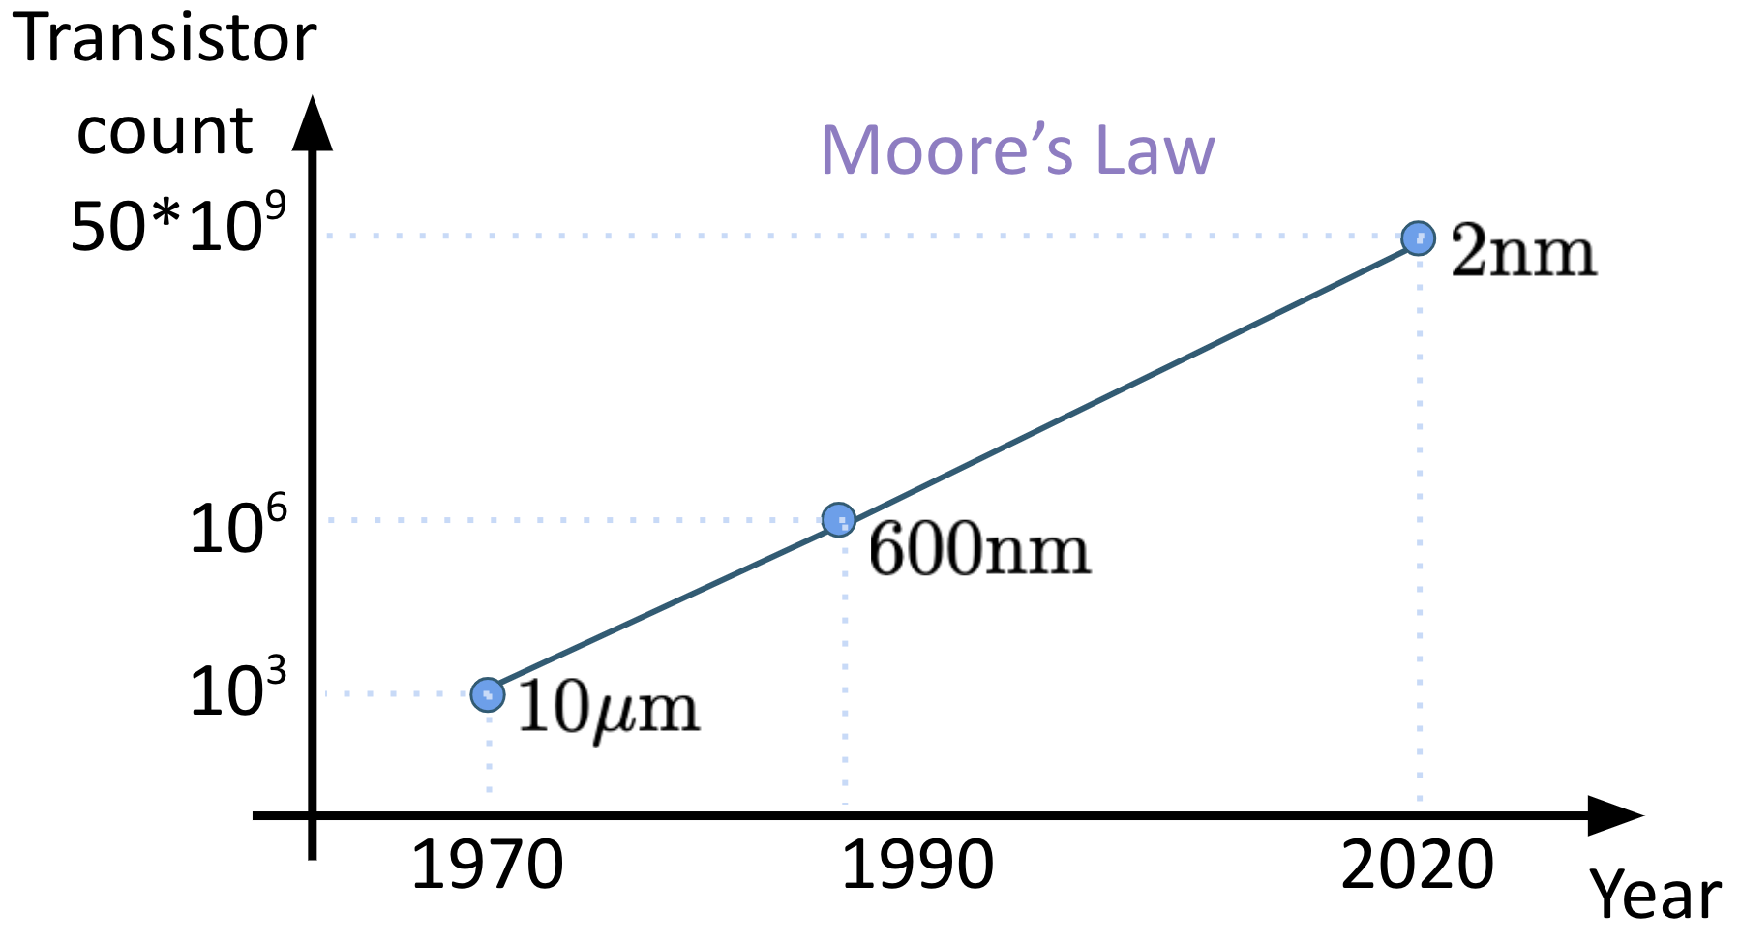
\includegraphics[width=0.8\textwidth]{lesson1/moore_law.pdf}
%     \label{fig:1-25}
%     \begin{center}
%         \caption{Moore's Law.}
%     \end{center}
% \end{figure}




% insert unencrytped msg pic (milk please)
% 

% insert credit card info 
% \begin{figure}[H]
%     \centering
%     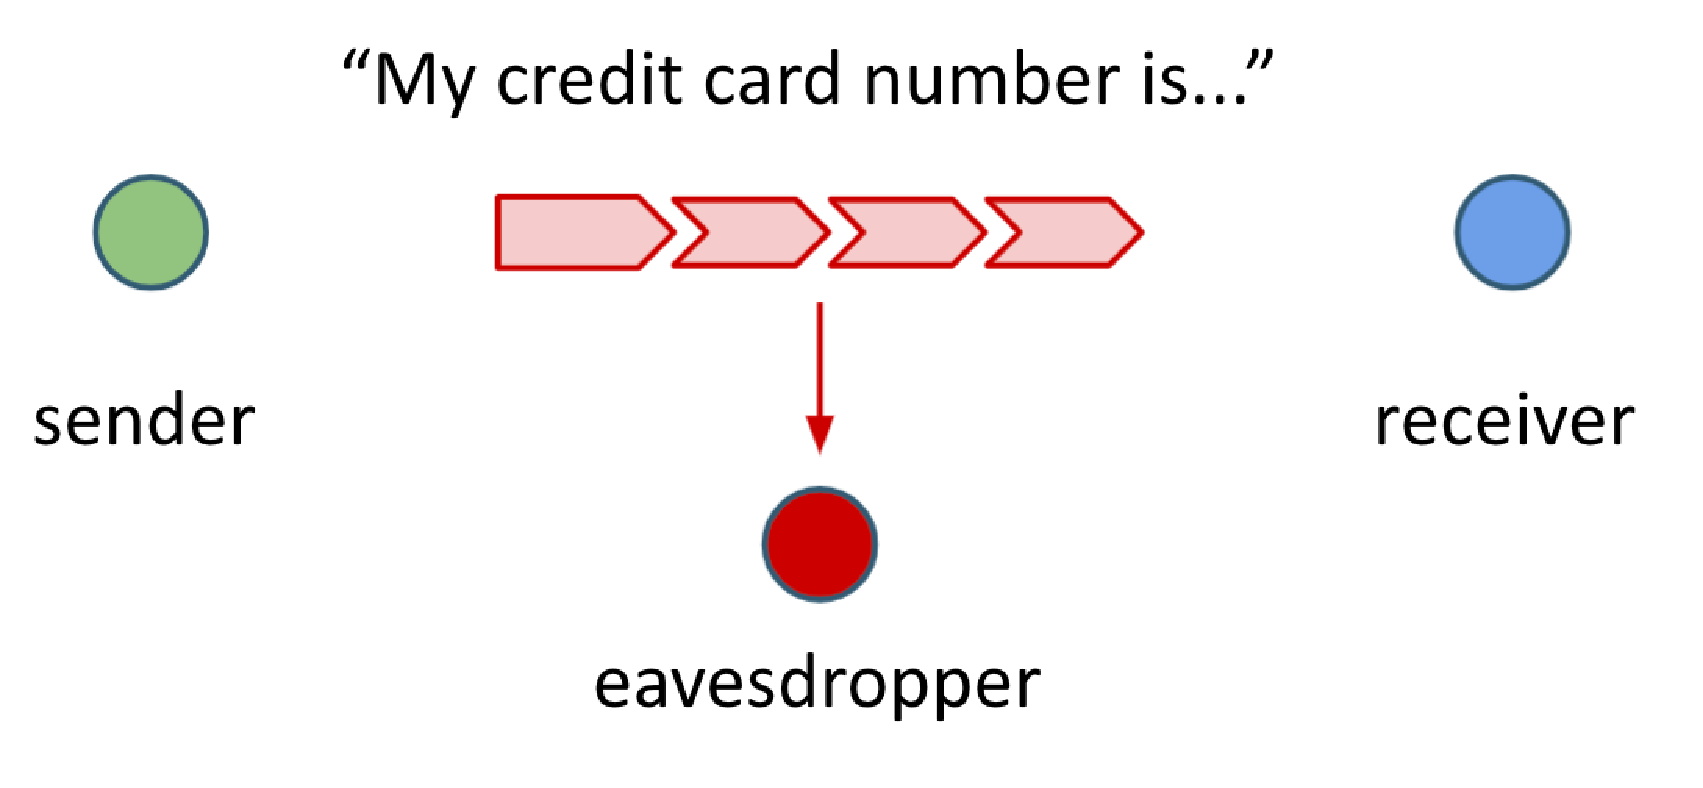
\includegraphics[width=0.8\textwidth]{lesson1/creditcardinfo.pdf}
%     \label{fig:1-26}
%     \begin{center}
%         \caption{Unencrypted communication: an eavesdropper overhearing your credit card information is much more likely to be a problem.}
%     \end{center}
% \end{figure}
% encrypted msg pic.
% \begin{figure}[H]
%     \centering
%     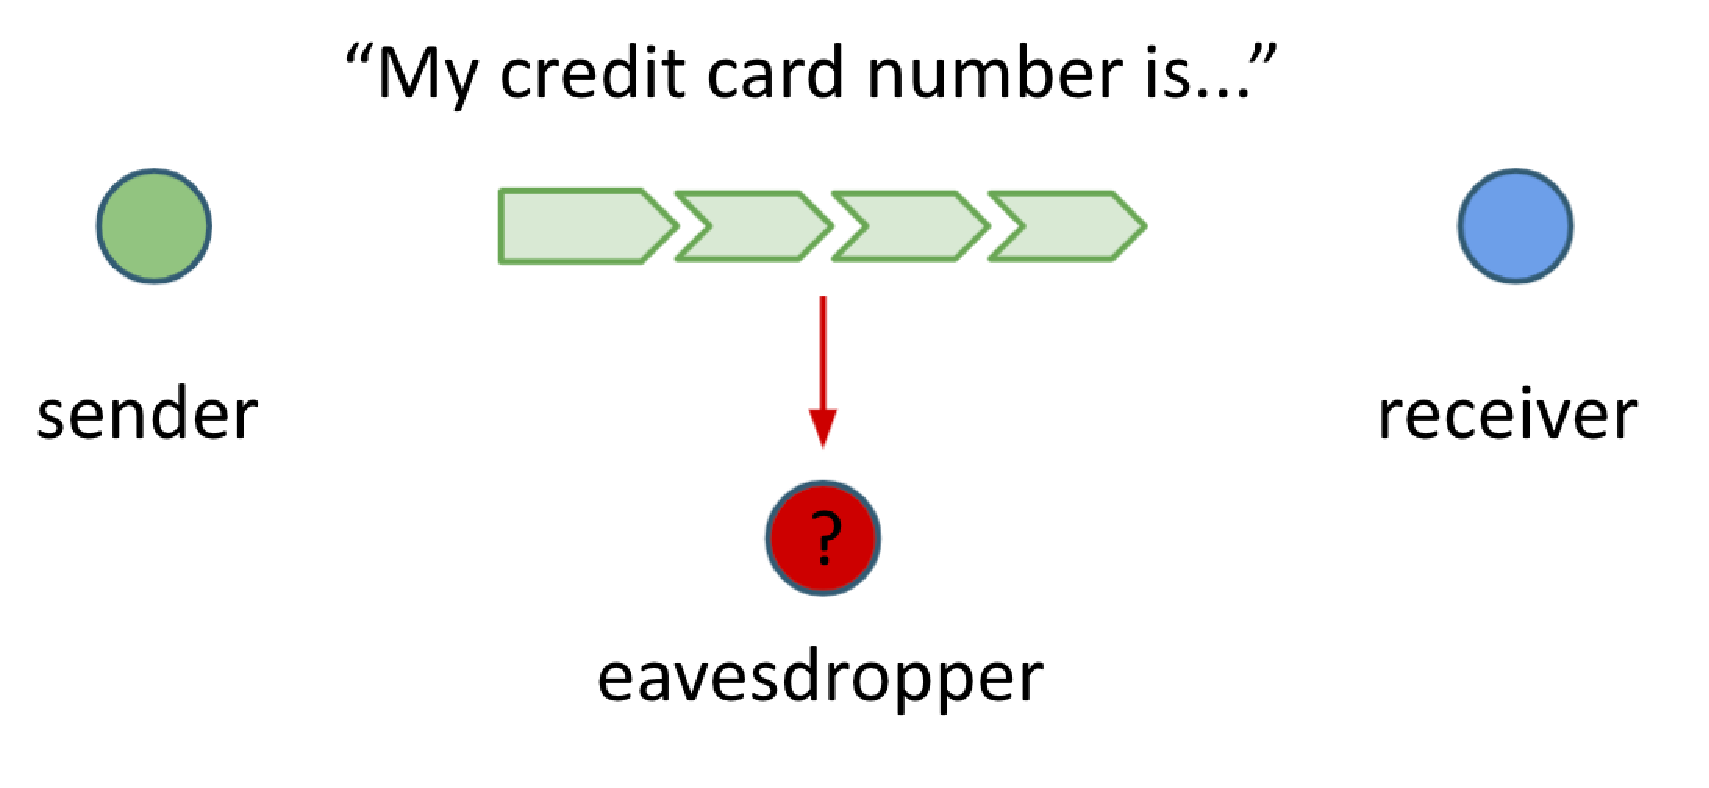
\includegraphics[width=0.8\textwidth]{lesson1/credit_card_info_eavesdropper.pdf}
%     \label{fig:1-28}
%     \begin{center}
%         \caption{Encrypted communication.}
%     \end{center}
% \end{figure}

% insecure channel pic.
% \begin{figure}[H]
%     \centering
%     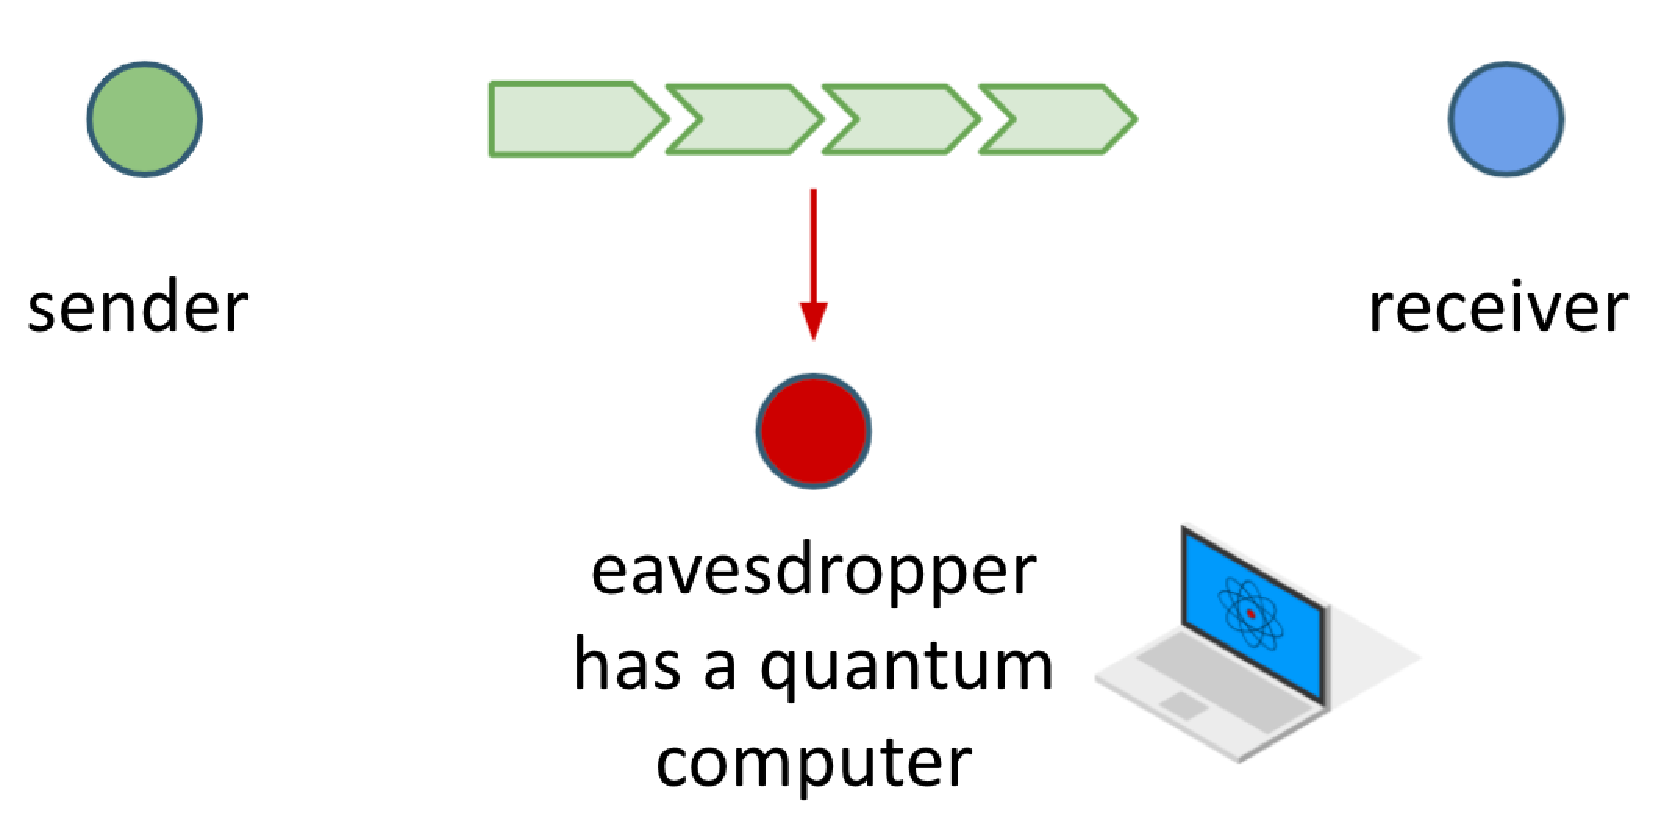
\includegraphics[width=0.8\textwidth]{lesson1/eavesdropper_Q_comp.pdf}
%     \label{fig:1-29}
%     \begin{center}
%         \caption{Eavesdropper with a quantum computer.}
%     \end{center}
% \end{figure}

% Quantum Channel "STOP" pic
% \begin{figure}[H]
%     \centering
%     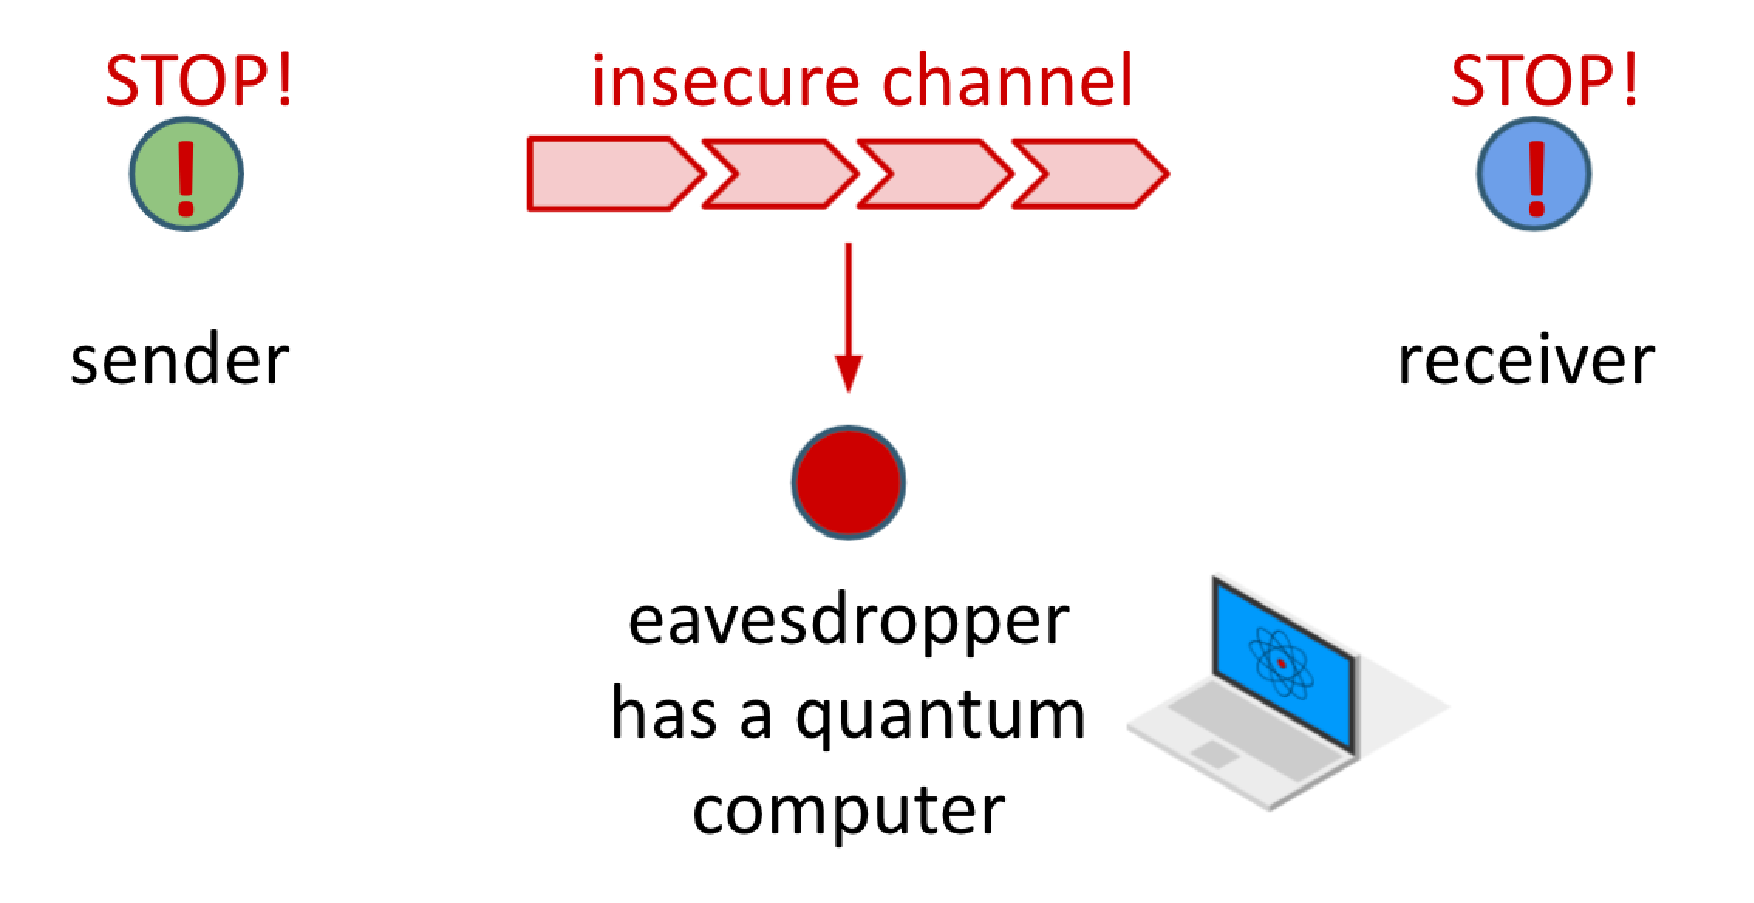
\includegraphics[width=0.8\textwidth]{lesson1/insecure_channel_stop.pdf}
%     \label{fig:1-30}
%     \begin{center}
%         \caption{Insecure quantum channel stops.}
%     \end{center}
% \end{figure}



% \section{(XXX Is a section break needed here?)}


% insert course overview pic
% \begin{figure}[H]
%     \centering
%     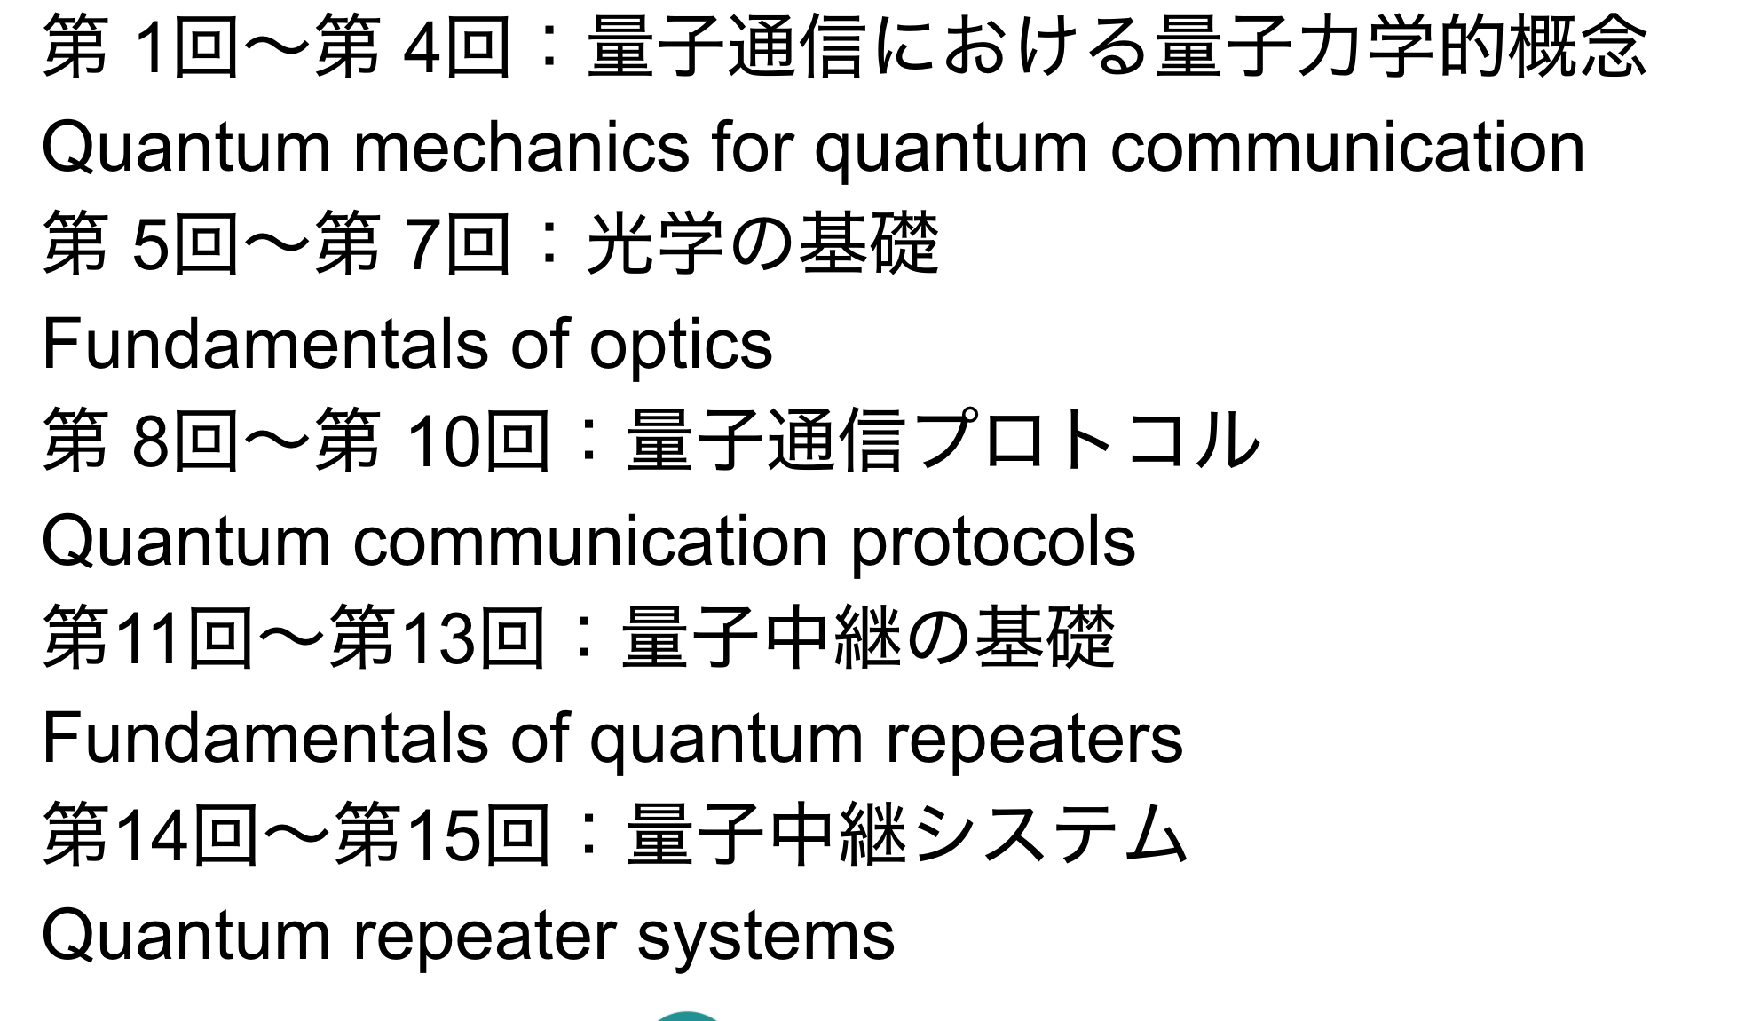
\includegraphics[width=0.8\textwidth]{lesson1/module_overview.pdf}
%     \label{fig:1-31}
%     \begin{center}
%         \caption{Module overview.}
%     \end{center}
% \end{figure}

% insert pre-requisities slide 
% \begin{figure}[H]
%     \centering
%     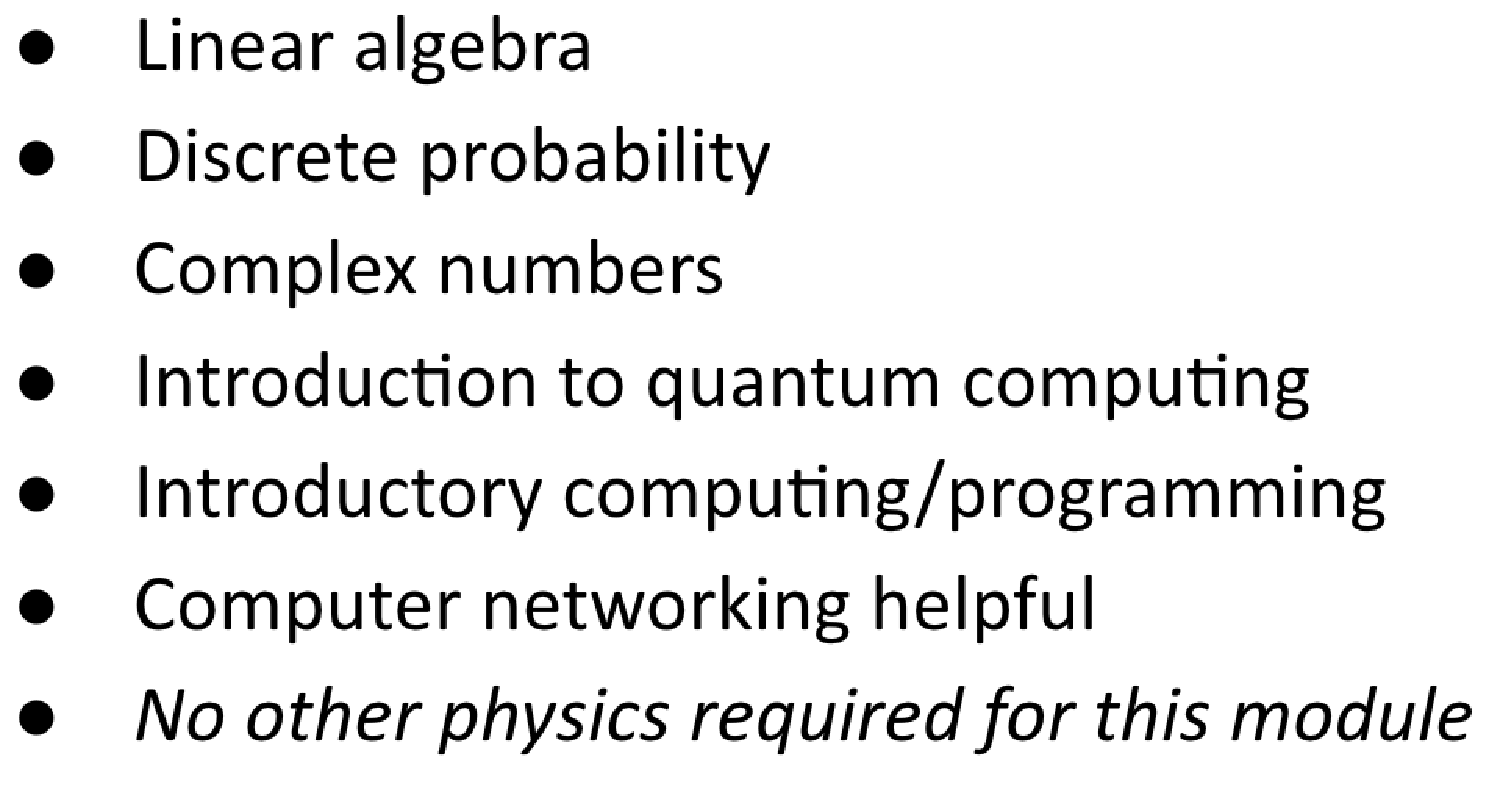
\includegraphics[width=0.8\textwidth]{lesson1/prereqs.pdf}
%     \label{fig:1-32}
%     \begin{center}
%         \caption{Prerequisites.}
%     \end{center}
% \end{figure}

% Rod videos pic
% \begin{figure}[H]
%     \centering
%     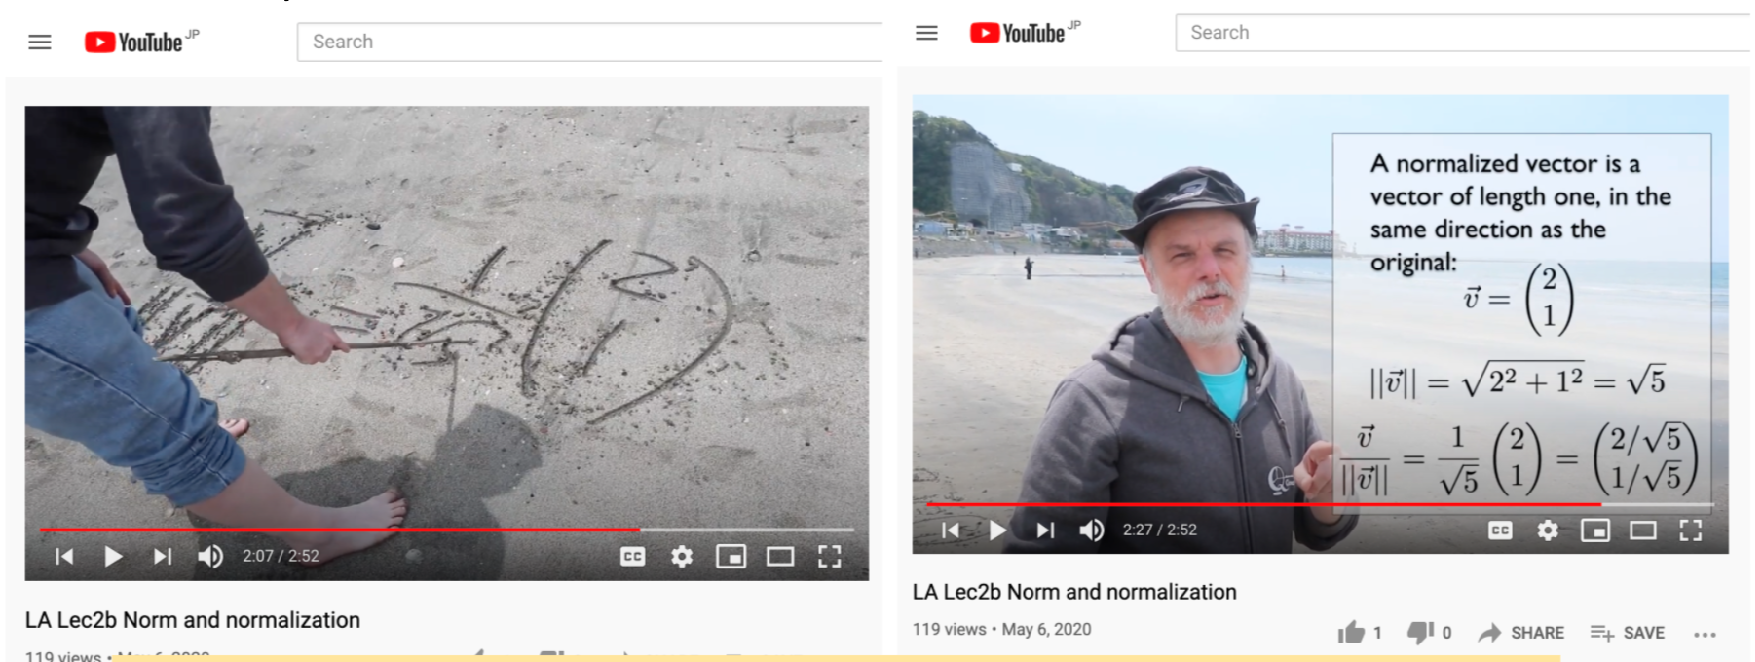
\includegraphics[width=1.1\textwidth]{lesson1/lin_alg_vids.pdf}
%     \label{fig:1-33}
%     \begin{center}
%         \caption{Linear Algebra videos.}
%     \end{center}
% \end{figure}

% \url{http://www.youtube.com/playlist?list=PLibMrvP9xUbeWZ1pCKnbTn2FO-c1PqHZr}.

% \newpage
% \begin{exercises}
% \exer{For Hooker's data, Exercise 1.2, use the Box and Cox and Atkinson procedures to determine a appropriate transformation of PRES
% in the regression of PRES on TEMP. find $\hat\lambda$, $\tilde\lambda$,
% the score test, and the added variable plot for the score. 
% Summarize the results.}

% \subexer{The following data were collected in a study of the effect of dissolved sulfur
% on the surface tension of liquid copper (Baes and Killogg, 1953).}


% \blankline
% \begin{tabular}{r@{}lcc}
% \hline
% &&\multicolumn2c{$Y$= Decrease in Surface Tension}\\
% \multicolumn2c{$x$ = Weight \% sulfur}
% &\multicolumn2c{(dynes/cm), two Replicates}\\
% \hline
% 0.&034&301&316\\
% 0.&093&430&422\\
% 011.&30&593&586\\
% \hline
% \end{tabular}
% \blankline

% \subexer{Find the transformations of $X$ and $Y$ sot that in the transformed scale 
% the regression is linear.}

% \subexer{Assuming that $X$ is transformed to $\ln(X)$, which choice of $Y$ gives 
% better results,
% $Y$ or $\ln(Y)$? (Sclove, 1972).}

% \sidebysidesubsubexer{In the case of $\Delta_1$?}{In the case of $\Delta_2$?}

% \exer{Examine the Longley data, Problem 3.3, for applicability of assumptions of the
% linear model.}

% \sidebysidesubexer{In the case of $\Gamma_1$?}{In the case of $\Gamma_2$?}
% \[
%     t= \frac{5}{256}\, \frac{c^5}{G^3}\,
%     \frac{r^4}{(m_1m_2)(m_1+m_2)}.  
% \]

% \end{exercises}


\chapter[Quantum States]{Quantum States}
\label{sec:2_quantum_states}


\chaptermark{Quantum States}

%\chapterauthor{Hein Mannaerts}

% \begin{abstract}
In this lesson, we will learn about quantum states: how to write them down, what they represent, and how they differ from classical states and bits.
Then, we will learn how to operate on, process, and extract information from quantum states using measurements. Lastly, we'll discuss multiple quantum states and how to describe them.  Most of this chapter will be familiar to those who have taken an introductory quantum computing course.

% \end{abstract}

\section{Qubits}

% \subsection*{2.1.1: Qubits (Quantum bit)}

Recall from Chapter 1 that all information can be represented by classical bits in the classical world. Classical bits are confined to either the zero or one states, whereas the qubit can be "in-between" zero or one in  \textbf{superposition} states. Mathematically, the general qubit state for a superposition of $\ket{0}$ and $\ket{1}$ is represented using notation known as \textbf{Dirac Notation}, written
\begin{equation}
\ket{\psi} = \alpha \ket{0} + \beta\ket{1} 
\end{equation}
 where $\ket{\cdot}$ is pronounced (\emph{ket}), $\psi$ (\emph{psi}) represents a general qubit state, $\alpha,\beta \in \mathbb{C}$.

%%%% taking out these three figures
\if0
% Insert qubit 100% 0
\begin{figure}[H]
    \centering
    \includegraphics[width=0.8\textwidth]{lesson2/100%0.pdf}
        \caption{100\% 0 qubit}
    \label{fig:100-zero}
\end{figure}

% Insert qubit 100% 1 
\begin{figure}[H]
    \centering
    
\includegraphics[width=0.8\textwidth]{lesson2/100_1.pdf}
    
        \caption{100\%1 qubit}
    
    \label{fig:100-one}
\end{figure}

% Insert superposition state pic.
\begin{figure}[H]
    \centering
    
\includegraphics[width=0.8\textwidth]{lesson2/superposition_qubit.pdf}
    
        \caption{A qubit in superposition}
    
    \label{fig:superpos}
\end{figure}
\fi
%%%%%% end of cut

% Dirac Notation w/ annotation
\begin{figure}[H]
    \centering
    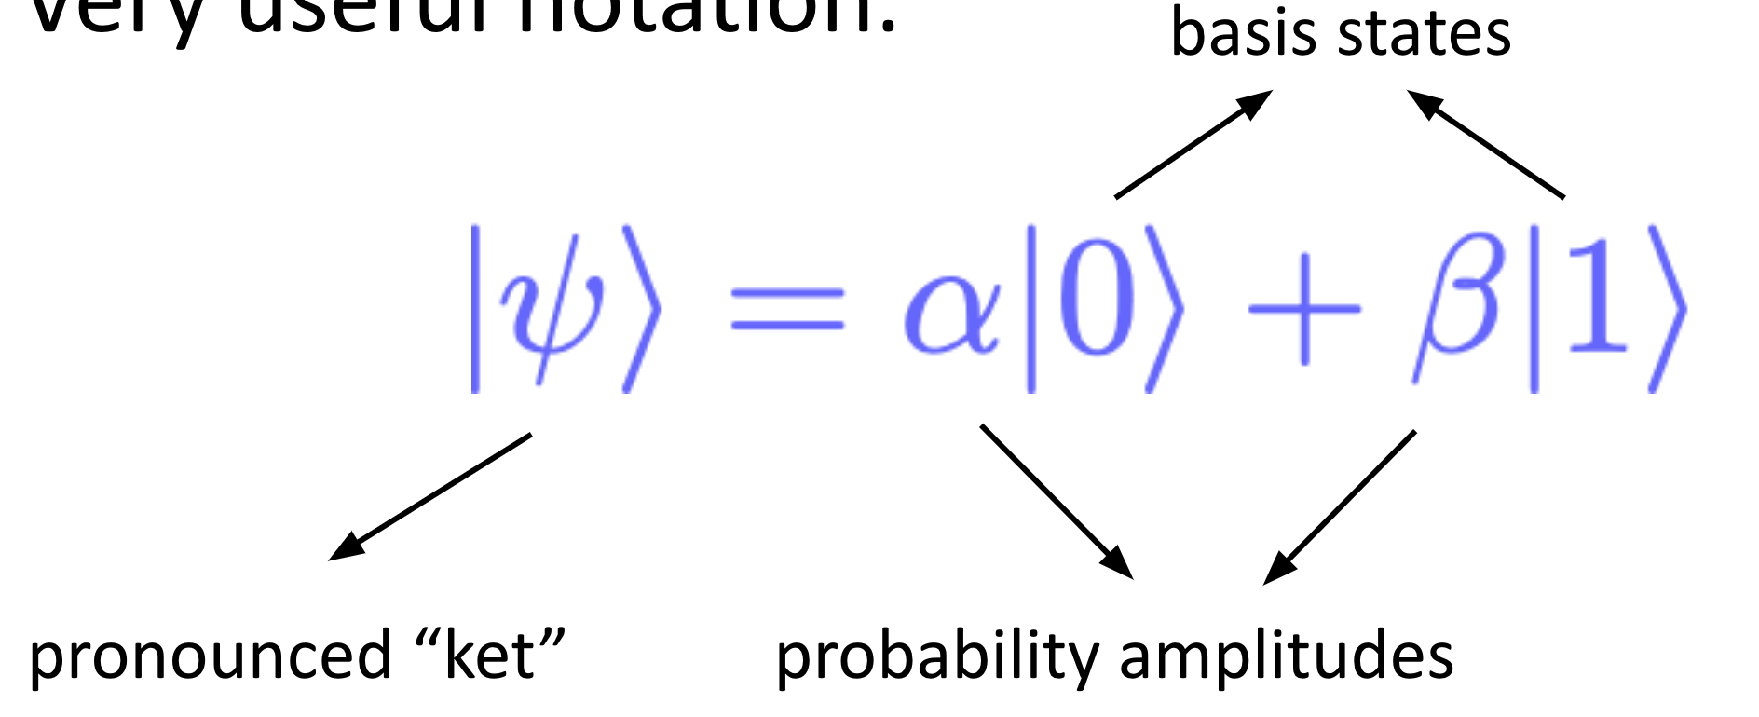
\includegraphics[width=0.8\textwidth]{lesson2/dirac_notation.pdf}
    
        \caption{Dirac ket notation. \rdv{This visual is probably helpful, needs to be redrawn or re-exported to get rid of that clipped text.}}
    
    \label{fig:ket-notation}
\end{figure}

% Bloch Sphere
\begin{figure}[H]
    \centering
    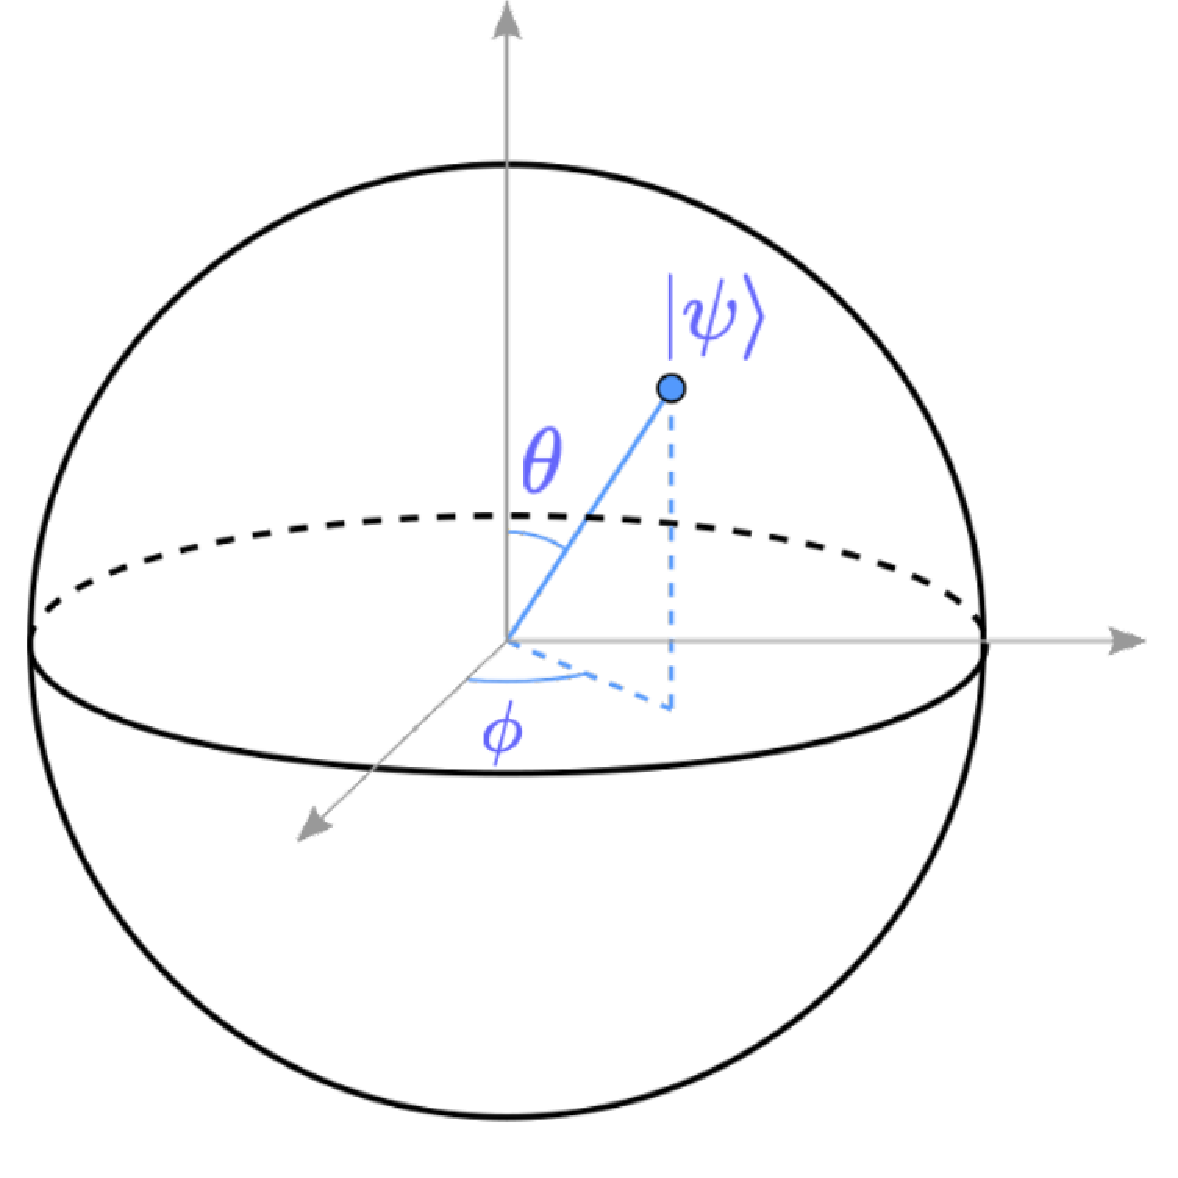
\includegraphics[width=0.6\textwidth]{lesson2/bloch_sphere.pdf}
    
        \caption{Bloch sphere}
    
    \label{fig:bloch}
\end{figure}

% insert Bloch sphere w/ axes labelled and |+> |-> meanings
\begin{figure}[H]
    \centering
    \includegraphics[width=0.7\textwidth]{lesson2/bloch_sphere_annotated.pdf}
    
        \caption{Bloch sphere with X, Y, and Z axis basis states.}
    
    \label{fig:annotated-bloch}
\end{figure}

%Hi, and welcome to lesson two on Quantum Mechanics for Quantum Communication. In this lesson, we will learn about quantum states. We will learn how to write them down, what they represent, and how they differ from classical states and particularly classical bits. 
%Then we will move on to learning how to operate quantum states, how to process them, how to extract information from them using measurements, and finally we will conclude by looking at multiple quantum states and how to describe them. So let's begin. 

First, let's discuss quantum bits, also known as \emph{qubits}. We have seen in the previous lesson that all the information can be represented by classical bits. In the classical world, you have zeros and you have ones, so a classical bit can only be in two states: it can either be in a zero, like here, or it can be fully in one, nothing in between. Whereas the quantum bit (as I said: a "qubit") can be anything in between. It can be a hundred percent zero, it can also be hundred percent one, but it can also be fifty percent zero and fifty percent one. Such a state is called a \emph{superposition}. It's not that we don't know what the state is, it really is neither 0 nor 1 but it's somewhere in between.

How do we write down a general quantum state of a qubit? Well the most common notation is called "Dirac notation"\index{Dirac notation}, and it's extremely useful. It's written like this,
\begin{align}
\ket{\psi} = \alpha\ket{0} + \beta\ket{1}
\end{align}
with this funny angle bracket, and this symbol $\psi$ (Greek letter "psi") is normally used to describe a general state of a quantum bit. So, this is pronounced the "ket" ($\ket{}$)\index{ket}, and we're going to be calling it "state psi" or "ket psi" interchangeably, and that is equal to a superposition of a zero and a one. $\ket{0}$ and $\ket{1}$ are called the "basis states", and they determine what our state is. This $\alpha$ and $\beta$ are "probability amplitudes" that tell us how much of the state is in zero and how much of the state is in one.  These probability amplitudes can be any complex number, provided that they satisfy this normalization condition:
\begin{align}
    |\alpha|^2 + |\beta|^2 = 1
\end{align}
(read "mod alpha squared plus mod beta squared is equal to one"). This is to ensure that whatever measurements we do in the future on this state we get correct probabilities out.

Another very useful representation of quantum states is using the \emph{Bloch sphere}\index{Bloch sphere}, as shown in Figs.~\ref{fig:bloch} and \ref{fig:annotated-bloch}. This visual representation gives us a very intuitive way of thinking about quantum states. So a Bloch sphere is a three-dimensional sphere. We have here the x-axis, here the y-axis, and the vertical is the z-axis, and all the states are given as points on the surface of the sphere, parameterized by the angle $\theta$ and the angle $\phi$. So then the state $\ket{\psi}$ can be written in the following form,
\begin{equation}
|\psi\rangle=\cos \frac{\theta}{2}|0\rangle+e^{i \phi} \sin \frac{\theta}{2}|1\rangle
\end{equation}
where the probability amplitude for basis state 0 is given by $\cos(\theta/2)$ and the probability amplitude for basis state 1 is given by the complex phase $e^{i \phi} \sin \frac{\theta}{2}$. 

This is a general state, but let's look at some examples. So we've got these states zero and one which we have already encountered, and they sit at the north and the south pole of the Bloch sphere. We also said that we can have an arbitrary superposition of zero and one. For example, we can have "plus state" which is given as equal superposition of zero and one, or we can have its friend on the other side of the block sphere the "minus state", which is an equal superposition but this time it's zero minus one, and equally we can also have two states on the y-axis, one is called the "plus i" the other one is "minus i", and they're given by this state here. You can see that again, it's an equal superposition of zero and one, but this time the phase between zero and one is given by a complex number "i".
This concludes step one.

\section{Unitary Operations}


% Classical (SSD) VS Quantum (Ion Trap)
\begin{figure}[H]
    \centering
    \includegraphics[width=0.9\textwidth]{lesson2/2-2_classical_quantum_info.pdf}
        \caption{A physical system.}
    \label{fig:physical-system}
\end{figure}

Let's see how we can manipulate quantum states, and therefore manipulate quantum information as well. We're going to do this with \emph{unitary operations}. One thing that you have to realize is that \emph{all information is physical}. This is because the information is represented by physical systems. Therefore, to change the information and process, it we have to interact with the physical systems that carry the information. For example, in classical information, you've got two very good examples in "HDDs (Hard disk drives)" where you read, write and manipulate information with very weak and precise magnetic fields, and for an example of a younger technology, we can look at the "solid-state drive" where you do the same thing, but you achieve it by manipulating very weak electric currents.

On the other hand in quantum information, you can look at physical systems such as \emph{ion traps}. For example, this ion trap from a company called IonQ, where individual atoms are represented by this blue dot. They're suspended on magnetic fields and they represent individual quantum bits, and you apply some pulses of lasers and you can manipulate the states of these qubits.  You can also look at \emph{superconducting qubits} from companies such as IBM or Google, where you can do the same thing. 

But how do we actually describe these transformations? Before we do that, let's look at some examples. The most simple transformation that we can think of is actually to do nothing, and we call this the \emph{identity operation} and it's usually represented by a capital $I$. When it's acting on a ket, it takes $\ket{0}$ to  $\ket{0}$  ($\ket{0}\rightarrow\ket{0}$) and $\ket{1}$ to $\ket{1}$ ($\ket{1}\rightarrow\ket{1}$). Classically, we can also do something similar by just not touching our classical bit. 0 remains 0 and 1 remains 1.

Another very simple operation is the \emph{flip}. Usually we call it either "flip" or a "Pauli X operation", and we represent it by a capital $X$, and it does exactly what you would expect. It takes the input $\ket{0}$ into an output $\ket{1}$, and vice versa, $\ket{1}$ into a $\ket{0}$. Again, classically you have a corresponding representation as well. It's the NOT gate, where it takes input 0 into classical bit 1 and bit 1 into classical bit 0. Also, we can create superpositions. This is known as the \emph{Hadamard operation}\index{Hadamard}, denoted by capital H. It takes as input the $\ket{0}$ and it outputs an equal superposition of 0 or 1 (0+1), or it can take in the input as 1 and output 0-1, and now you see this is the first example of a quantum operation that doesn't really have a classical analog. As we said, we cannot have superpositions of classical bits.

So what's the definition of a unitary operation? All of these examples that we consider, they are examples of unitary operations. Any unitary operation has the property of being reversible, that means we can undo it. We can reverse its effect, and this is done by what's known as an "adjoint" denoted as $U^\dagger$ ("U dagger") where "U" is the unitary.
So let's see how that works. We start with a ket $\ket{\psi}$ and we apply a unitary that transforms it into a completely new ket $\ket{\psi'}$, and then if we apply the adjoint so the operation which undoes the effect of the original unitary, we end up back again at the state $\ket{\psi}$. So we can write $\ket{\psi}$ prime is equal to the unitary U applied to $\ket{\psi}$, or we can also write ket $\ket{\psi}$ is equal to the adjoint of the unitary applied to $\ket{\psi}$ prime. 

Let's put these two together. We start with our input state $\ket{\psi}$. We apply the $U^\dagger$ (U dagger) which is the same as applying the adjoint to the state $\ket{\psi'}$. But then again, we know the expression for $\ket{\psi'}$ from over here. So we can just substitute it in and we get U dagger times U times the state $\ket{\psi}$, and that's it! You see that in order for these sides to be equal, we must conclude that U dagger times U is the identity operator, and that makes logical sense. We are undoing the operation U with the adjoint, so the total effect of these two is we are doing nothing. Similarly, we can do it for $\ket{\psi}$ prime which is equal to U applied to $\ket{\psi}$, and again we substitute for $\ket{\psi}$ this expression over here, and we get a similar expression as above: U times U dagger times the state $\ket{\psi'}$. So from that we can see that also what needs to be true is that U times U dagger is equal to the identity operator, and that's precisely the definition of unitary operations. There you go, that U times U dagger must be equal to U dagger times U, and that is equal to the identity. 

%Let's move on. 
How can we represent this in matrix representation? So far we have been talking about states as these kets, but in fact they can be represented as vectors and we know that in order to transform vectors we have to multiply them by matrices, therefore unitary operations can be represented by matrices. So let's look at some examples. First let's begin with states. Usually we denote $\ket{0}$ in vector notation as a column vector 1 and 0,
\begin{equation}
\ket{0}\equiv\left(\begin{array}{l}
1 \\
0
\end{array}\right).
\end{equation}
The $\ket{1}$, on the other hand, is a column vector of 0 and 1,
\begin{equation}
\ket{1}\equiv\left(\begin{array}{l}
0 \\
1
\end{array}\right).
\end{equation}
So that then you can see that any general state $\ket{\psi}$ can be represented as $\alpha$ times the vector $\left(\begin{array}{l}
1 \\
0
\end{array}\right)$ plus $\beta$ times $\left(\begin{array}{l}
0 \\
1
\end{array}\right)$. In other words, it can just be represented as a complex column vector $$\left(\begin{array}{l}
\alpha \\
\beta
\end{array}\right)$$.

Now let's look at examples of some matrices and unitary operations. The identity operator is represented by the matrix
\begin{equation}
I=\left(\begin{array}{ll}
1 & 0 \\
0 & 1
\end{array}\right).
\end{equation}
It's just a diagonal matrix. It has ones on the main diagonal and zeros everywhere else.

An important set of operations we will use many times is known as the set of \emph{Pauli operators}. We have encountered one Pauli operator already, the $X$ operator, which flips our ket from zero to one and from one to zero, but there are two other very important Pauli operators: the $Y$ and the $Z$, and they have these matrix representations, and also for completeness we also have the Hadamard operator~\footnote{The symbol $H$ can also represent an operator known as the \emph{Hamiltonian} of a system.  Hopefully it will be clear from context which one we mean, once we have introduced the Hamiltonian.} that creates a superposition, written $H$.  The matrices corresponding to these operators are

\begin{equation}
\begin{aligned}
&X=\left(\begin{array}{ll}
0 & 1 \\
1 & 0
\end{array}\right) \\
&Y=\left(\begin{array}{cc}
0 & -i \\
i & 0
\end{array}\right) \\
&Z=\left(\begin{array}{cc}
1 & 0 \\
0 & -1
\end{array}\right)
\end{aligned}
\end{equation}

\begin{equation}
H=\frac{1}{\sqrt{2}}\left(\begin{array}{cc}
1 & 1 \\
1 & -1
\end{array}\right)
\end{equation}


Let's see some examples just to give you a little bit of feeling for how this can actually work in practice. For the flip operation, you take the Pauli X, you apply it, or multiply it, by $\ket{0}$,

\begin{equation}
\begin{aligned}
X|0\rangle &=\left(\begin{array}{ll}
0 & 1 \\
1 & 0
\end{array}\right)\left(\begin{array}{l}
1 \\
0
\end{array}\right) \\
&=\left(\begin{array}{l}
0 \\
1
\end{array}\right)=|1\rangle
\end{aligned}
\end{equation}

%So we see that 0 times 1 is 0, plus 1 times 0 is 0. So we get a 0 here in this first element of this new column vector, but then we have 1 times 1 plus 0 times 0 which is 1, and you see that this is actually our ket 1, so it indeed did flip a 0 into 1 as we would expect.

We can do the same thing for $\ket{1}$. Again, you multiply the matrix representation of the Pauli $X$ operator with the column vector representation of state $\ket{1}$,
\begin{equation}
\begin{aligned}
X|1\rangle &=\left(\begin{array}{ll}
0 & 1 \\
1 & 0
\end{array}\right)\left(\begin{array}{l}
0 \\
1
\end{array}\right) \\
&=\left(\begin{array}{l}
1 \\
0
\end{array}\right)=|0\rangle
\end{aligned}
\end{equation}
and you get as expected $\ket{0}$. 

To create a superposition, take the Hadamard operator, apply it to the state $\ket{0}$. When you go through the algebra, in the end what you get is an equal superposition of 0 and 1. Please notice that this factor in the Hadamard operator, $1/\sqrt{2}$, ensures that the superposition vector at the end is properly normalized. If we take this number in front of zero, and it's also in front of one, and we take the mod squared of both, and we add them, it has to be one. Half plus half is equal to one, therefore this vector is correctly normalized. You can follow the same process for the state 1, and again as we have seen in the previous step you get zero minus one: again an equal superposition.

Now, we mentioned this "adjoint". So far it's been a rather abstract notion that can undo the effect of a unitary operation. How can we actually systematically compute this adjoint given a unitary matrix? It's actually very simple. There are two steps to it. You take the complex conjugate of the matrix. Just to remind you, the complex conjugate of a complex number "x plus iy star", which is the notation for complete conjugation, is equal to "x minus iy",
\begin{equation}
(x+i y)^{*}=x-i y
\end{equation}
 So wherever you see $i$, you just flip its sign and that's your complex conjugate.
 
So that's step number one: first take the complex conjugate of the matrix. Step two: take the transpose. The transpose of the matrix is given as follows: so for any matrix $U$ which has elements $U_{00}$, $U_{01}$, $U_{10}$ and $U_{11}$, transposing them will exchange the off-diagonal elements. So let's see how this unitary $U$ actually turns into an adjoint. First we apply the complex conjugation, so we take each element and we write a little star, denoting that this element is complex conjugated, and then we apply the transpose.
\begin{equation}
U=\left(\begin{array}{ll}
U_{00} & U_{01} \\
U_{10} & U_{11}
\end{array}\right) \rightarrow\left(\begin{array}{cc}
U_{00}^{*} & U_{01}^{*} \\
U_{10}^{*} & U_{11}^{*}
\end{array}\right) \longrightarrow\left(\begin{array}{ll}
U_{00}^{*} & U_{10}^{*} \\
U_{01}^{*} & U_{11}^{*}
\end{array}\right)=U^{\dagger}
\end{equation}
You see that I have flipped these off-diagonal elements, but I have not touched the diagonal elements, and that's your U-dagger, your adjoint operation. In particular, if you look at an example given by unitary Pauli Y matrix written as this, first we take the complex conjugate so zero is just zero but the signs in front of these off-diagonal elements change because they're pure imaginary, and then we flip them because we're applying the transpose and we get the same matrix Y. When this happens, when the adjoint of a unitary matrix is equal to the unitary matrix, we say that that matrix is self-adjoint and we will see many examples where this is, in fact, true.

\begin{equation}
Y=\left(\begin{array}{cc}
0 & -i \\
i & 0
\end{array}\right) \longrightarrow\left(\begin{array}{cc}
0 & i \\
-i & 0
\end{array}\right) \longrightarrow\left(\begin{array}{cc}
0 & -i \\
i & 0
\end{array}\right)=Y
\end{equation}

Another very important class of unitary operations are \emph{rotations} and this is where the Bloch sphere representation will be extremely handy. The rotation can be written in this strange looking form (strange for now), and what it means is that we are rotating around some arbitrary direction in the Bloch sphere by some arbitrary angle $\theta$, and we write this as this following exponent.

\begin{equation}
R_{\hat{n}}(\theta)=e^{-i \theta \hat{n} \cdot \hat{\sigma} / 2}
\end{equation}

\begin{equation}
e^{-i \theta \hat{n} \cdot \hat{\sigma} / 2 }=\cos \frac{\theta}{2} I-i \sin \frac{\theta}{2}\left(n_{x} X+n_{y} Y+n_{z} Z\right)
\end{equation}

\begin{equation}
R_{\hat{n}}(\theta)|\psi\rangle=\left|\psi^{\prime}\right\rangle
\end{equation}

Here, $\hat{n}$ (read "n hat") is just a unit length vector given by coordinates $n_x$, $n_y$ and $n_z$, and this vector given by $\hat{\sigma}$ ("sigma hat") is just a vector of our Pauli matrices $X$, $Y$ and $Z$. So we can write this as follows: this exponential decomposes into cosine theta over 2 times the identity matrix minus i times sine theta 2, and then this expression which is just the dot product between these two vectors, so we multiply $n_x$ by Pauli matrix $X$, plus $n_y$ times Pauli matrix $Y$, plus $n_z$ times Pauli matrix $Z$. It does look a little bit complicated, but in the Bloch sphere representation it becomes very clear what's going on. 


% insert Bloch sphere rotation y-axis
\begin{figure}[H]
    \centering
    \includegraphics[width=0.7\textwidth]{lesson2/bloch_y_axis.pdf}
    
        \caption{Rotation about the Y axis}
    
    \label{fig:y-rot}
\end{figure}

Let's consider an example, as shown in Fig.~\ref{fig:y-rot}: we want to rotate around the y-axis given by the horizontal axis in the figure, through an angle of $\pi/2$, and our initial state is given by $\ket{0}$.  Let's start at the point $\ket{0}$, at the north pole of the sphere, and we just rotate around the y-axis. We are going down along the surface by angle $\pi/2$, and you see that we reach the state $\ket{+}$, which is an equal superposition of 0 and 1.  Written out, we have
\begin{equation}
R_{Y}(\pi / 2)\ket{0}=\ket{+}.
\end{equation}

\begin{figure}[H]
    \centering
    \includegraphics[width=0.7\textwidth]{lesson2/bloch_general_axis.pdf}
    
        \caption{Rotation about an arbitrary axis}
    
    \label{fig:arb-rot}
\end{figure}

More generally, you don't have to rotate about any of these orthogonal axes, you can rotate about any axis that you want, as in Fig.~\ref{fig:arb-rot}. You are rotating in this plane parameterized by this angle $\theta$, so it takes some initial state $\ket{\psi}$ that's on the surface of the Bloch sphere, it follows the surface and it ends in some new state $\ket{\psi'}$. 

So you can see that you can work in the matrix representation or you can work also in the Bloch sphere representation.

% Simple Unitary Operations 
\begin{figure}[H]
    \centering
    \includegraphics[width=0.7\textwidth]{lesson2/simple_unitary_ops.pdf}
    
        \caption{A simple unitary transform}
    
    \label{fig: 1}
\end{figure}

\begin{equation}
|\psi\rangle=U^{\dagger}\left|\psi^{\prime}\right\rangle=U^{\dagger} U|\psi\rangle
\end{equation} 

\begin{equation}
\left|\psi^{\prime}\right\rangle=U|\psi\rangle=U U^{\dagger}\left|\psi^{\prime}\right\rangle
\end{equation}

\begin{equation}
U U^{\dagger}=U^{\dagger} U=I
\end{equation}

becomes
\begin{equation}
|\psi\rangle=\alpha\left(\begin{array}{l}
1 \\
0
\end{array}\right)+\beta\left(\begin{array}{l}
0 \\
1
\end{array}\right)=\left(\begin{array}{l}
\alpha \\
\beta
\end{array}\right).
\end{equation}

\begin{equation}
\begin{aligned}
H|0\rangle &=\frac{1}{\sqrt{2}}\left(\begin{array}{cc}
1 & 1 \\
1 & -1
\end{array}\right)\left(\begin{array}{l}
1 \\
0
\end{array}\right) \\
&=\frac{1}{\sqrt{2}}\left(\begin{array}{l}
1 \\
1
\end{array}\right)=\frac{1}{\sqrt{2}}(|0\rangle+|1\rangle)
\end{aligned}
\end{equation}

\begin{equation}
\begin{aligned}
H|1\rangle &=\frac{1}{\sqrt{2}}\left(\begin{array}{cc}
1 & 1 \\
1 & -1
\end{array}\right)\left(\begin{array}{l}
0 \\
1
\end{array}\right) \\
&=\frac{1}{\sqrt{2}}\left(\begin{array}{c}
1 \\
-1
\end{array}\right)=\frac{1}{\sqrt{2}}(|0\rangle-|1\rangle)
\end{aligned}
\end{equation}

% $U_{00}$, $U_{01}$, $U_{10}$, $U_{11}$ 

\section{Measurement}

Now, let's consider measurements and how they can extract information from quantum qubits. So how does it work? Basically a measurement asks the question: is my state in the state $\ket{0}$ or is it in the state $\ket{1}$? You can think of a measurement as a big box and you feed it your prepared state, as shown in Fig.~\ref{fig:z-measure}. Here, we consider a general state given by $\ket{\psi} = \alpha\ket{0}+\beta\ket{1}$, and the measurement operation tells you which state it is in. Usually there are only two possible values that can come out of a measurement device, which we will assign the values $+1$ and $-1$.

\begin{figure}[H]
    \centering
    \includegraphics[width=0.7\textwidth]{lesson2/Pauli_z_machine.pdf}
    
        \caption{Measurement in the Z basis}
    
    \label{fig:z-measure}
\end{figure}

The probabilities of these measurement outcomes, corresponding to state zero and state one, are given by their probability amplitudes. The probability of getting a $+1$ outcome is given by $|\alpha|^2$ and the probability of a $-1$ outcome is given by $|\beta|^2$. Immediately after the measurement, the state \emph{collapses} either onto a zero or onto a one, so if you get a plus one outcome you can be sure that immediately after the measurement the state is in the state zero, or if you get a minus one then the state of the system has changed from the initial $\ket{\psi}$ and is one,
\begin{align}
\operatorname{Prob}\{+1\}=|\alpha|^2 \rightarrow \textrm{state is } |0\rangle \\
\operatorname{Prob}\{-1\}=|\beta|^2 \rightarrow \textrm{state is } |1\rangle.
\end{align}

We refer to this particular measurement as a measurement in the \emph{computational basis} or in the Pauli $Z$ basis. This already hints at the fact that this is not the only measurement we can do. We can, in fact ask the following question: is the state in the $\ket{+}$ state or in the $\ket{-}$ state? We can answer this question by rewriting our original state
\begin{equation}
|\psi\rangle=\alpha|0\rangle+\beta|1\rangle
\end{equation}
using the algebraic identities
\begin{equation}
|0\rangle=\frac{1}{\sqrt{2}}(|+\rangle+|-\rangle) \quad|1\rangle=\frac{1}{\sqrt{2}}(|+\rangle-|-\rangle).
\end{equation}
Notice that $\ket{0}$ is given by an equal superposition of the $\ket{+}$ state with the $\ket{-}$ state and the state $\ket{1}$ is \emph{also} an equal superposition of $\ket{+}$ and $\ket{-}$, but this time with a minus phase in front of the $\ket{-}$ state. We can rewrite our original state $\ket{\psi}$ in terms of these plus and minus states, but this time the probability amplitudes for the state plus is $\alpha+\beta$ renormalized by the square root of two, and the probability amplitude for the minus state is $\alpha-\beta$,
\begin{equation}
|\psi\rangle=\frac{\alpha+\beta}{\sqrt{2}}|+\rangle+\frac{\alpha-\beta}{\sqrt{2}}|-\rangle.
\end{equation}
Again, we can feed our qubit into the measurement device and it will give us an answer $\ket{+}$ or $\ket{-}$ with the following probabilities,
\begin{align}
\operatorname{Prob}\{+1\}=\frac{|\alpha+\beta|^2}{2} \rightarrow \textrm{state is } |+\rangle \\
\operatorname{Prob}\{-1\}=\frac{|\alpha-\beta|^2}{2} \rightarrow \textrm{state is } |-\rangle.
\end{align}
You can see that the probabilities still depend on $\alpha$ and $\beta$, but they're not just $|\alpha|^2$ and $|\beta|^2$.
%they're in fact alpha plus beta the whole thing mod squared and alpha minus beta the whole thing squared and both of them are divided by two. 
And again because we were asking a different question (whether the state state is in $\ket{+}$ or $\ket{-}$), then the state changes from $\ket{\psi}$ and goes to $\ket{+}$ or $\ket{-}$ after the measurement depending on the measurement outcome. This measurement is known as measurement in the Pauli X basis.  In fact, you can measure in any basis that you can think of.  

I've been using this word \emph{basis}, but what is a "basis"? Maybe you remember from your linear algebra class that the basis is a set of vectors that allows you to write down any vector that you can think of. In particular, if we have some general vector $\ket{\psi}$, we can write it in the Pauli Z basis given by $\ket{0}$ and one, and already we have talked about the vector representations for $\ket{0}$ and one. And then the state in Dirac notation is written as follows, or you can write it in a new basis. Let's say you want to write it in terms of these states $\ket{i}$ and $\ket{-i}$. This is known as the Pauli Y basis, and their vector representations are given as
\begin{align}
    |i\rangle=\frac{1}{\sqrt{2}}\left(\begin{array}{l}1 \\ i\end{array}\right) \quad|-i\rangle=\frac{1}{\sqrt{2}}\left(\begin{array}{c}1 \\ -i\end{array}\right).
\end{align}
%So it's just (1, i) and (1, -i) with the appropriate normalization factor in front, and 
Then the state can be rewritten as
\begin{equation}
|\psi\rangle=\frac{\alpha-i \beta}{\sqrt{2}}|i\rangle+\frac{\alpha+i \beta}{\sqrt{2}}|-i\rangle.
\end{equation}
These two vectors look very different but they represent the same state: the state has not changed, it's just that our description of the state is a little bit different because we have chosen a different basis in which to describe it.

Another very important concept is the \emph{inner product}\index{inner product}. The inner product is basically a dot product between two vectors, just as you probably learned in your basic linear algebra class, but to talk about it in our notation first we have to define a \emph{bra}\index{bra}. Given a state $\ket{\psi}$, we can write down its bra, which is just its adjoint. So the bra of state $\ket{\psi}$ is given as the dagger of the original column vector,
\begin{equation}
\langle\psi|=(|\psi\rangle)^{\dagger}=\left(\begin{array}{l}
\alpha \\
\beta
\end{array}\right)^{\dagger}=\left(\begin{array}{ll}
\alpha^{*} & \beta^{*}
\end{array}\right).
\end{equation}
You apply the same trick as we applied for defining the adjoint of unitaries: you take the complex conjugate of $\alpha$ and $\beta$ and then you transpose the column vector, which turns it into a row vector. Now you can find the inner product between two arbitrary states, $\ket{\psi} = \alpha\ket{0} + \beta\ket{1}$ and $\ket{\phi} = \gamma\ket{0} + \delta\ket{1}$. Then we write it as 
%this: so we have bra times the ket in vector representation it's given by this. We have the row vector of
%(gamma star, delta star) multiplying the column vector (alpha, beta) and you get this following expression out:
\begin{equation}
\langle\phi \mid \psi\rangle=\left(\begin{array}{ll}
\gamma^{*} & \delta^{*}
\end{array}\right)\left(\begin{array}{c}
\alpha \\
\beta
\end{array}\right)=\alpha \gamma^{*}+\beta \delta^{*}.
\end{equation}
This should be no surprise if you remember your dot products from your linear linear algebra class.

Also notice that if you take the inner product of the state with itself, you in fact get this expression:
\begin{equation}
\langle\psi \mid \psi\rangle=|\alpha|^{2}+|\beta|^{2}=1
\end{equation}
Mod alpha squared plus mod beta squared will be equal to one, if the state is properly normalized. For two different states, you can also come across the scenario where the inner product between two states is zero,
\begin{equation}
\langle\phi \mid \psi\rangle=0.
\end{equation}
In that case, we say that the two states are \emph{orthogonal}.
%, just like in your classical linear algebra class between normal vectors.

How do we obtain these probabilities for the measurement outcomes? We have stated them as a fact before, but now you will see how to actually get them. We have our general state $\ket{\psi}$, and we say that we want to measure in some arbitrary basis $\ket{b_0}$ and $\ket{b_1}$. We are asking the question: is my state in the state $b_0$ or is my state in the state $b_1$? This is where the inner product comes in. We take the inner product between $\ket{b_0}$ and $\ket{\psi}$, we take the modulus and we square it, and that gives us the probability of a $+1$ outcome, and correspondingly the probability of the $-1$ outcome is given by the inner product between $\ket{b_1}$ and $\ket{\psi}$ modulus squared,
\begin{equation}
\begin{aligned}
\operatorname{Prob}\{+1\}&=\left|\left\langle b_{0}\mid \psi\right\rangle\right|^{2} \\
\operatorname{Prob}\{-1\}&=\left|\left\langle b_{1}\mid \psi\right\rangle\right|^{2}.
\end{aligned}
\end{equation}

To illustrate this with some simple examples, we're going to measure in the Pauli Z basis, and again, the probability of outcome one is given by mod alpha squared and probability of minus one is given by mod beta squared,
\begin{equation}
\begin{aligned}
\operatorname{Prob}\{+1\} &=|\langle 0 \mid \psi\rangle|^2 \\
&=|\alpha|^2 \\
\operatorname{Prob}\{-1\} &=|\langle 1 \mid \psi\rangle|^2 \\
&=|\beta|^2.
\end{aligned}
\end{equation}

How about measuring in our Pauli Y basis? Well again, probability of $+1$ is given by the modulus of alpha minus i beta the whole thing squared over two, and the probability of the minus one outcome is given by modulus of alpha plus i beta squared divided by two,
\begin{equation}
\begin{aligned}
\operatorname{Prob}\{+1\} &=|\langle i \mid \psi\rangle|^2 \\
&=\frac{|\alpha-i \beta|^2}{2} \\
\operatorname{Prob}\{-1\} &=|\langle-i \mid \psi\rangle|^2 \\
&=\frac{|\alpha+i \beta|^2}{2}.
\end{aligned}
\end{equation}

To summarize the measurement process, you start with some initial state written in some basis,
%here I have written it in the computational or in the Pauli Z basis, 
and then you say, okay I want to perform a measurement in a given basis described by these basis states $\ket{b_0}$ and $\ket{b_1}$. If my outcome is $+1$, which happens with the probability given by the inner product between the basis state with the original state modulus squared, then my post measurement state is given by $\ket{b_0}$. Or, if I get the $-1$ outcome, which happens with probability given by the inner product of $\ket{b_1}$ with the initial state $\ket{\psi}$ modulus squared, then my post measurement state is given by $\ket{b_1}$. But there is something very important to keep in mind: the measurement outcome is only $+1$ or $-1$. It does not give you any information about these probability amplitudes $\alpha$ and $\beta$. In the next section, we will see more about those probability amplitudes.


% と表示できます。1の状態だったらマイナスの状態には位相をつけるでしょう。
\begin{figure}[H]
    \centering
    \includegraphics[width=0.7\textwidth]{lesson2/Pauli_x_machine.pdf}
    
        \caption{Measurement in the X basis}
    
    \label{fig:x-meas}
\end{figure}

% Insert basis representation pic here.
\begin{figure}[H]
    \centering
    \includegraphics[width=0.7\textwidth]{lesson2/basis_representation.pdf}
    
        \caption{Basis state representation}
    
    \label{fig:bases}
\end{figure}

%%%%%%%%%%%%%%%%%%
\if0
\begin{figure}[H]
    \centering
    \includegraphics[width=0.5\textwidth]{lesson2/Pauli_z_ex.pdf}
    
        \caption{Probability in Z basis measurement}
    
    \label{fig: 1}
\end{figure}

% Pauli Y example
\begin{figure}[H]
    \centering
    \includegraphics[width=0.5\textwidth]{lesson2/Pauli_y_ex.pdf}
    
        \caption{Probability in Y axis measurement}
    
    \label{fig: 1}
\end{figure}
\fi
%%%%%%%%%%%%%%%%%%

\section{Probabilities, expectation, variance}

We have seen how measurements can be applied to quantum states, but now let's see how we can actually extract information about the probabilities and the expectation values and variances of these measurements. Up to this point, we have only measured one single qubit as an individual event, as in Figs.~\ref{fig:z-measure} and \ref{fig:x-meas}.  This is known as \emph{single shot measurement}. Now let's consider the scenario where we have many copies of the same state and we keep measuring them again and again and again, as shown in Fig.~\ref{fig:many-copies}. We have our measurement device and we keep feeding it the same state: many copies of state $\ket{\psi}$. What comes out is a bit string of $+1$ and $-1$ results.

We can count the number of $+1$ outcomes, which we will denote by $N(+1)$, and we can count the number of $-1$ outcomes, which we will denote by $N(-1)$. Intuitively, the ratio between the number of $+1$ outcomes to the total number of measurements will be approximately equal to the probability of obtaining the plus one outcome, which is $|\alpha|^2$, and similarly for the fraction of the number of $-1$ outcomes, which will be very close to $|\beta|^2$,

\begin{equation}
\begin{aligned}
&\frac{N(+1)}{N(+1)+N(-1)} \approx|\alpha|^{2} \\
&\frac{N(-1)}{N(+1)+N(-1)} \approx|\beta|^{2}.
\end{aligned}
\end{equation}

In order to extract any information about the probabilities, we have to repeat the same measurement on a fresh copy of your state again and again and again. Because these measurements are random, we're not going to get the same answer every time. However, we can ask the question: what is the expected result when I measure in the Pauli Z basis? What number should I get if I repeat the same measurement many many times? Maybe you remember from your probability course that the \emph{expectation value} of some random variable is the sum of the probability of each possible outcome times its value. Let's call our variable $Z$ because we are measuring in the Pauli Z basis.  Its expectation value is given by the probability of the $+1$ outcome times $+1$ (the value of the outcome), plus the probability of $-1$ times the value of the outcome, which is in this case $-1$.  The probability of $+1$ remains $|\alpha|^2$, and the probability of the $-1$ outcome is given by $|\beta|^2$, but this time we are multiplying it by $-1$. So the expectation value when we measure in the Pauli Z basis is given by the expression
\begin{equation}
\begin{aligned}
\mathbb{E}[Z] &=\operatorname{Prob}(+1) \cdot(+1)+\operatorname{Prob}(-1) \cdot(-1) \\
&=|\alpha|^{2}-|\beta|^{2}.
\end{aligned}
\end{equation}

In Dirac notation we write it as follows: we write the operator in which basis we are measuring and we enclose it in the angle brackets, but really it's just a shorthand for saying that we are multiplying the bra of state $\bra{\psi}$ times the $Z$ operator times the ket of state $\ket{\psi}$,

\begin{equation}
\langle Z\rangle=\langle\psi|Z| \psi\rangle.
\end{equation}

Let's check it: take the Pauli Z operator and sandwich it between our state given by the column vector $\alpha$ and $\beta$. Its bra is given by a row vector, so we've got the row vector $\ket{\psi}$ times Pauli Z matrix times the column vector $\ket{\psi}$. When we multiply it out, we get the following expression which agrees with the expectation value that we have computed above.
\begin{equation}
\begin{aligned}
\langle Z\rangle &=\left(\begin{array}{ll}
\alpha^{*} & \beta^{*}
\end{array}\right)\left(\begin{array}{cc}
1 & 0 \\
0 & -1
\end{array}\right)\left(\begin{array}{l}
\alpha \\
\beta
\end{array}\right) \\
&=\left(\begin{array}{ll}
\alpha^{*} & \beta^{*}
\end{array}\right)\left(\begin{array}{c}
\alpha \\
-\beta
\end{array}\right) \\
&=|\alpha|^{2}-|\beta|^{2}
\end{aligned}
\label{eq:z-expectation}
\end{equation}

Again, because the number of the measurements are random we expect some degree of variance in our measurement outcomes, and again we use the same definition as from classical probability theory that the variance of some random variable is given by the expectation value of the square of that variable, minus the square of the expectation value of that variable,
\begin{equation}
\begin{aligned}
\operatorname{Var}[Z] &=\mathbb{E}\left[Z^{2}\right]-\mathbb{E}[Z]^{2}.    
\end{aligned}
\end{equation}
We have already computed the expectation value of Z, we don't need to do that anymore, we just square the expression from Eq.~\ref{eq:z-expectation}. Now we have to compute the expectation value of $Z^2$. That's the probability of getting a $+1$ outcome times $(+1)^2$ which is just $+1$.  The probability of the $-1$ outcome times $(-1)^2$, which is $1$, so actually what we get is
\begin{equation}
\begin{aligned}
\mathbb{E}\left[Z^{2}\right] &=\operatorname{Prob}\{+1\} \cdot(+1)^{2}+\operatorname{Prob}\{-1\} \cdot(-1)^{2} \\
&=|\alpha|^{2}+|\beta|^{2}.
\end{aligned}
\end{equation}

Often in physics you will see that the variance is referred to as \emph{fluctuations}, and that's denoted by $(\Delta Z)^2$ and that's really just the variance of Z. In the Dirac notation, we again have this expression,
\begin{equation}
\begin{aligned}
(\Delta Z)^{2} & \equiv \operatorname{Var}[Z] \\
&=\left\langle Z^{2}\right\rangle-\langle Z\rangle^{2}.
\end{aligned}
\end{equation}


% many copies machine
\begin{figure}[H]
    \centering
    \includegraphics[width=0.5\textwidth]{lesson2/many_copies_machine.pdf}
    
        \caption{Multiple measurements}
    
    \label{fig:many-copies}
\end{figure}


\section{Multiple Qubits}
\label{sec:multi-qubit}

Now, let's consider how to write down the state of multiple qubits. So how do we write down the state of two bits? Let's start with a very simple question like that. Well, if we have two classical bits, they can be in four different states. They can be in $00$, $01$, $10$, or $11$. So what's the case for quantum bits? We need to switch to the Dirac notation. We can have the $\ket{00}$, $\ket{01}$, $\ket{10}$, and $\ket{11}$. Any general state of two qubits can be written as a superposition of these four states weighted by some probability amplitudes. We need four of them because we have four different states: $\alpha$, $\beta$, $\gamma$ and $\delta$, 
\begin{equation}
|\psi\rangle=\alpha|00\rangle+\beta|01\rangle+\gamma|10\rangle+\delta|11\rangle
\end{equation}
and again the state must be normalized such that when we measure, it gives the correct probabilities. But this time the normalization condition is as follows: it's mod of all the probability amplitude squared, when you sum it up it has to be equal to one again,
\begin{equation}
|\alpha|^2+|\beta|^2+|\gamma|^2+|\delta|^2 = 1.
\end{equation}
And again in vector notation, we can write these kets as follows: $\ket{00}$ now is a column vector of four elements: (one, zero, zero, zero), and similarly for $\ket{01}$, $\ket{10}$, and $\ket{11}$,
\begin{equation}
|00\rangle=\left(\begin{array}{l}
1 \\
0 \\
0 \\
0
\end{array}\right),|01\rangle=\left(\begin{array}{l}
0 \\
1 \\
0 \\
0
\end{array}\right),|10\rangle=\left(\begin{array}{l}
0 \\
0 \\
1 \\
0
\end{array}\right),|11\rangle=\left(\begin{array}{l}
0 \\
0 \\
0 \\
1
\end{array}\right).
\end{equation}
So you see that this is a nice orthogonal basis with which we can express any general state $\ket{\psi}$. In fact, we can now write our combination of those amplitudes above as a vector,
\begin{equation}
\ket{\psi}=\alpha\left(\begin{array}{l}
1 \\
0 \\
0 \\
0
\end{array}\right) + \beta\left(\begin{array}{l}
0 \\
1 \\
0 \\
0
\end{array}\right)+\gamma\left(\begin{array}{l}
0 \\
0 \\
1 \\
0
\end{array}\right)+\delta\left(\begin{array}{l}
0 \\
0 \\
0 \\
1
\end{array}\right)=\left(\begin{array}{l}
\alpha \\
\beta \\
\gamma \\
\delta
\end{array}\right).
\end{equation}

The very important mathematical concept behind being able to write the basis states like that is that of a \emph{tensor product}\index{tensor product}~\footnote{There are actually multiple types of tensor products; by one definition, a tensor is like an $n$-dimensional matrix instead of the customary two-dimensional one.  In this book, we will use tensors in a fashion that expands the vector or matrix size, instead of making it into a multidimensional object.}.

So how do we actually get these two new qubit basis states? We took some state of the first qubit, let's call it "a" because it can be anything, and we took a tensor product with another qubit state "b". Mathematically, you have a column vector for the first qubit given by these probability amplitudes $a_1$ and $a_2$ tensor product the column vector for the second qubit $b_1$ $b_2$, and this operation of the tensor product is defined as follows:

\begin{equation}
|a\rangle \otimes|b\rangle=\left(\begin{array}{l}
a_{1} \\
a_{2}
\end{array}\right) \otimes\left(\begin{array}{l}
b_{1} \\
b_{2}
\end{array}\right) \equiv\left(\begin{array}{l}
a_{1}\left(\begin{array}{l}
b_{1} \\
b_{2}
\end{array}\right) \\
a_{2}\left(\begin{array}{l}
b_{1} \\
b_{2}
\end{array}\right)
\end{array}\right)=\left(\begin{array}{l}
a_{1} b_{1} \\
a_{1} b_{2} \\
a_{2} b_{1} \\
a_{2} b_{2}
\end{array}\right)
\end{equation}

\if0
$
\left(\begin{array}{l}
a_1 \\
a_2
\end{array}\right)$
%のベクトルと
$\left(\begin{array}{l}
b_1 \\
b_2
\end{array}\right)$
\fi

To calculate the product, take the first probability amplitude $a_1$ times the whole column vector for $\ket{b}$. That will give you the first two elements in your new four dimensional vector.  $a_1$ times $b_1$ goes into the first entry in the resulting vector, $a_1$ times $b_2$ goes in the second entry, and then for the bottom two elements you take $a_2$ and again you multiply the whole column vector of $\ket{b}$, so you have $a_2$ times $b_1$ and $a_2$ times $b_2$.

In ket notation, we have $\ket{a} \otimes \ket{b}$, which can be represented in vector form. For example, if we have two qubits and the first qubit is in state $\ket{0}$ and the second qubit is in state one, we write it as column vectors and take the tensor product like this,
%(1 0) tensor product (0 1), and you can see that one times zero is zero, one times one is one, zero times zero is zero, and finally zero times one is zero,
\begin{equation}
|0\rangle \otimes|1\rangle=\left(\begin{array}{l}
1 \\
0
\end{array}\right) \otimes\left(\begin{array}{l}
0 \\
1
\end{array}\right)=\left(\begin{array}{l}
0 \\
1 \\
0 \\
0
\end{array}\right).
\end{equation}

Similarly, we can take the tensor product of more complicated states: we have tensor product of $\ket{1}$ with $\ket{-}$,
%so we have the column vector (0 1) tensor product this superposition with an extra minus phase in here, so it's one over square root of two, times the column vector one minus one, and that gives us this two-qubit state (0, 0, 1, -1), all renormalized by this one over square root of two,
\begin{equation}
|1\rangle \otimes|-\rangle=\left(\begin{array}{l}
0 \\
1
\end{array}\right) \otimes \frac{1}{\sqrt{2}}\left(\begin{array}{c}
1 \\
-1
\end{array}\right)=\frac{1}{\sqrt{2}}\left(\begin{array}{c}
0 \\
0 \\
1 \\
-1
\end{array}\right).
\end{equation}

The tensor product is very general; if you have two vectors with $m$ and $n$ entries, their tensor product will be a vector with $mn$ entries in it. When dealing with qubits, our vectors will generally have a length that is a power of two; each qubit you add to the system doubles the number of entries in the vector when we take the tensor product.

Also, for our purposes, the length of each individual vector is normalized, and the tensor product retains this property.

Finally, be careful: just as with ordinary matrix products, the order of vectors (kets) written in a tensor product matters. This will be explored in detail in the exercises.

How do we actually apply tensor products to matrices so that we can describe operations on multiple qubits? It's a very similar logic: we have two matrices "A" and "B", we take the tensor product between them. We take the first element $A_{11}$ of the first matrix and we multiply the entire second matrix by that value. This will give us the upper left region of the new four by four matrix. 

\begin{equation}
\begin{aligned}
A \otimes B &=\left(\begin{array}{ll}
A_{11} & A_{12} \\
A_{21} & A_{22}
\end{array}\right) \otimes\left(\begin{array}{ll}
B_{11} & B_{12} \\
B_{21} & B_{22}
\end{array}\right) \\
&=\left(\begin{array}{lll}
A_{11}\left(\begin{array}{ll}
B_{11} & B_{12} \\
B_{21} & B_{22}
\end{array}\right) & A_{12}\left(\begin{array}{ll}
B_{11} & B_{12} \\
B_{21} & B_{22}
\end{array}\right) \\
A_{21}\left(\begin{array}{ll}
B_{11} & B_{12} \\
B_{21} & B_{22}
\end{array}\right) & A_{22}\left(\begin{array}{ll}
B_{11} & B_{12} \\
B_{21} & B_{22}
\end{array}\right)
\end{array}\right) \\
&=\left(\begin{array}{llll}
A_{11} B_{11} & A_{11} B_{12} & A_{12} B_{11} & A_{12} B_{12} \\
A_{11} B_{21} & A_{11} B_{22} & A_{12} B_{21} & A_{12} B_{22} \\
A_{21} B_{11} & A_{21} B_{12} & A_{22} B_{11} & A_{22} B_{12} \\
A_{21} B_{21} & A_{21} B_{22} & A_{22} B_{21} & A_{22} B_{22}
\end{array}\right)
\end{aligned}
\end{equation}

%%%%%%%% no need for this one
\if0
\begin{figure}[H]
    \centering
    \includegraphics[width=0.8\textwidth]{lesson2/matrix_tensor.pdf}
    
        \caption{Matrix tensor}
    
    \label{fig:tensor-unused}
\end{figure}
\fi
%%%%%%%%%% end no need


In the upper left, we have $A_{11}$ times the matrix representation of $B$. In the upper right square, we have the element $A_{12}$ times the whole matrix $B$. In the lower left, we have  $A_{21}$ times matrix $B$, and finally in the lower right $A_{22}$ times matrix $B$. If you multiply out the whole equation, you can see that you have to calculate many individual matrix elements, or you can see that it's way simpler to write an equation in Dirac notation.

As an example, consider an operation on two qubits, applying an $X$ to our first (left) qubit, while leaving the second (right) qubit alone. This would be written as
\begin{equation}
\begin{aligned}
(X \otimes I)|\psi\rangle &=X \otimes I(\alpha|00\rangle+\beta|01\rangle+\gamma|10\rangle+\delta|11\rangle) \\
&=\alpha|10\rangle+\beta|11\rangle+\gamma|00\rangle+\delta|01\rangle
\end{aligned}
\end{equation}
If we write out the tensor of the operators, we have
\begin{equation}
(X \otimes I)=\left(\begin{array}{ll}
0 & 1 \\
1 & 0
\end{array}\right) \otimes\left(\begin{array}{ll}
1 & 0 \\
0 & 1
\end{array}\right)=\left(\begin{array}{llll}
0 & 0 & 1 & 0 \\
0 & 0 & 0 & 1 \\
1 & 0 & 0 & 0 \\
0 & 1 & 0 & 0
\end{array}\right).
\end{equation}

We can also see how to distribute independent operations. If we want to apply the operator $A$ to the state $\ket{a}$ and the operator $B$ to the state $\ket{b}$, we can apply the tensor conveniently before or after applying the operators to the states,
%We write the A tensor product B, operating on the ket "a" tensor product with "b", can be written as A- matrix A applied to ket a tensor product matrix B acting on ket b. 
\begin{equation}
(A \otimes B)|a\rangle \otimes|b\rangle=A|a\rangle \otimes B|b\rangle.
\end{equation}

Note that, unlike ordinary matrix multiplication, two matrices being tensored do not have to have a dimension in common. They can be any size. If $A$ is an $l\times m$ matrix and $B$ is an $n \times p$ matrix, the result will be an $ln \times mp$ matrix.

A note on notation: when tensoring kets, we can leave out the $\otimes$ symbol and just write $\ket{a}\ket{b}$ with the same meaning as $\ket{a}\otimes\ket{b}$. We cannot do the same with matrices, however, as that would be ambiguous with ordinary matrix multiplication.

Finally, by now you have probably recognized that one of the great advantages of the Dirac notation is its compactness. Two qubits can have four possible states, three qubits can have eight possible states, and so on; for $n$ qubits, the state vector is $2^n$ elements long when written out. But most of the time, we don't need to write out the entire state.  You have seen that the individual basis states are more compactly written, such as writing $\ket{00}$ instead of the whole four-element vector, let alone writing out the whole sixteen elements of the four-qubit state $\ket{0000}$. But more generally, even when dealing with an arbitrary state $\ket{\psi}$, we only need to write out the \emph{nonzero} elements, allowing us to ignore the zero elements.  Thus, a four-qubit superposition of the all-zeroes and all-ones states only requires us to write $\ket{\psi} = (\ket{0000} + \ket{1111})/\sqrt{2}$, saving our hands, our pens, and ultimately being easier cognitively as well~\footnote{If you are familiar with the execution of matrix math in high-performance computing, the Dirac and tensor notations are equivalent to a \emph{sparse representation}, keeping a list of nonzero elements instead of all of them.}.

\if0
$\left(\begin{array}{ll}
1 & 0 \\
0 & 1
\end{array}\right)$

$\left(\begin{array}{ll}
0 & 1 \\
1 & 0
\end{array}\right)$
\fi

\newpage
\begin{exercises}
\exer{Consider the following quantum state:}
\begin{equation*}
\ket{\psi} = \frac{\sqrt{3}}{2}\ket{0} + \frac{1}{2}\ket{1}
\end{equation*}
\subexer{Find the probability of measuring a zero.}
\subexer{Find the probability of measuring a one.}
\exer{Write out the vectors corresponding to the following tensor products. Confirm that the vectors remain normalized. Note that the order of writing the qubits matters, but the order of taking the products does not.} \subexer{$\ket{+}\otimes \ket{1}$.}
\subexer{$\ket{1}\otimes \ket{+}$.}
\subexer{$\ket{+}\otimes \ket{+}$.}
\subexer{$\ket{-}\otimes \ket{+}$.}
\subexer{$\ket{+}\otimes \ket{-}$.}
\subexer{$\ket{-}\otimes \ket{-}$.}
\subexer{$\ket{0}\otimes \ket{0} \otimes\ket{0}$.}
\subexer{$\ket{0}\otimes \ket{0} \otimes\ket{1}$.}
\subexer{$\ket{0}\otimes \ket{1} \otimes\ket{0}$.}
\subexer{$\ket{1}\otimes \ket{0} \otimes\ket{0}$.}
\subexer{$\ket{1}\otimes \ket{1} \otimes\ket{1}$.}
\subexer{$\ket{1}\otimes \ket{+} \otimes\ket{0}$.}

\exer{Write out the matrices corresponding to the following tensor products.} \subexer{$X\otimes X$.}
\subexer{$Z\otimes Z$.}
\subexer{$I\otimes X$.}
\subexer{$I\otimes Z$.}
\subexer{$X\otimes Z$.}
\subexer{$Z\otimes X$.}

\exer{Find the expectation value $\langle Z\rangle$ for the following single-qubit states.}
\subexer{$\ket{0}$}
\subexer{$\ket{1}$}
\subexer{$\ket{+}$}
\subexer{$\ket{-}$}
\subexer{$\frac{\sqrt{3}}{2}\ket{0} + \frac{1}{2}\ket{1}$}

\exer{Since we can find the expectation value of $Z$, you might suspect that we can do the same for $X$. Find the expectation value $\langle X\rangle$ for the following single-qubit states.}
\subexer{$\ket{0}$}
\subexer{$\ket{1}$}
\subexer{$\ket{+}$}
\subexer{$\ket{-}$}
\subexer{$\frac{\sqrt{3}}{2}\ket{0} + \frac{1}{2}\ket{1}$}

\end{exercises}


\chapter[Pure and Mixed States]{Pure and Mixed States}
\label{sec:3_pure_mixed}

This lesson will expand on what we learned in the previous lesson.
It will deal with pure and mixed states, and finally we will get to the description of real noisy quantum states.
The notation and mathematical tools that we develop in this this lesson will be extremely useful in the rest of these lecture notes.

\section{Noisy world}
\label{sec:3-1_noisy_world}

In this step, we will talk about the noisy world.
Up until now, we have only discussed quantum states which were noiseless, meaning they
were always in the exact state that we wanted them to be.
There was no uncertainty in our knowledge of the description of the state.
The world, however, is a noisy place and this description is not quite sufficient for real-world applications.
Let's consider three examples demonstrating why this is the case.

The first example is that of \textit{\textbf{state preparation}} as shown in Fig.~\ref{fig:3-1_noise}.
You may go to your friend who works in a quantum laboratory and ask him or her to prepare
a state $\ket{\psi}$.
What happens in a real lab is that the prepared
state is not the desired state $\ket{\psi}$.
If you are lucky it might be some other pure state $|\psi'\rangle$ which is close to the desired state $|\psi\rangle$.
You would still obtain a pure state, albeit not exactly the one you asked for, but at least you would have full knowledge of this state $|\psi'\rangle$.
Much more likely scenario is that your friend in the lab can only produce a distribution of pure states.
This means that we obtain some pure state $|\psi_1\rangle$ with probability $p_1$, or some pure state $|\psi_2\rangle$ with probability $p_2$, and so on and so forth.

The second example is that of \textit{\textbf{processing of information}}.
In this case we wish to perform a quantum computation represented by some unitary operator $U$.
Even if the input to the computation is an ideal pure state $|\psi\rangle$, the output will not be the desired $U|\psi\rangle$.
The output might contain coherent errors, meaning that the applied operation was some other unitary $U'$, giving us the output $U'|\psi\rangle$.
The output might be affected by incoherent errors, such as probabilistic Pauli errors, or relaxation errors.

\begin{figure}[t]
    \centering
    \includegraphics[width=\textwidth]{lesson3/3-1_noise.pdf}
    \caption[Noisy world]{Real quantum states are noisy.}
    \label{fig:3-1_noise}
\end{figure}

The last example deals with the central scenario of these lecture notes, namely \textit{\textbf{quantum communication}}.
Consider the case where you prepare a state $|\psi\rangle$, which you would like to send to a friend through a long optical fiber.
Even though we do not process the prepared state in any way, optical fibers themselves are sources of noise.
The state received by your friend will be affected by coherent and incoherent errors.
On top of these, the state may even get lost and never arrive.
This is due to various processes such as absorption or scattering in the fiber.
Photon loss is a huge headache in quantum communication and we will discuss it in more detail in later lessons.





\section{Outer product}
\label{sec:3-2_outer_product}

We have seen in the previous lesson that the inner product of two vector states $|a\rangle$ and $|b\rangle$ is formed by transforming the first ket into a bra and then multiplying them together,
\begin{equation}
    \langle a | b\rangle = \begin{pmatrix} a_0^* & a_1^* \end{pmatrix} \begin{pmatrix} b_0 \\ b_1 \end{pmatrix} = a_0^* b_0 + a_1^* b_1.
\end{equation}
This is nothing else but a generalization of the usual vector dot product to complex vectors.

What happens when we change the order of multiplication?
Let's multiply the ket $|b\rangle$ from the right by the bra $\langle a|$,
\begin{equation}
    | b\rangle \langle a | = \begin{pmatrix} b_0 \\ b_1 \end{pmatrix} \begin{pmatrix} a_0^* & a_1^* \end{pmatrix} = \begin{pmatrix} a_0^*b_0 & a_1^*b_0 \\ a_0^*b_1 & a_1^*b_1 \end{pmatrix}.
\end{equation}
By changing the order of multiplication, we obtained a complex matrix.
The above product of a ket with a bra is called an \textit{\textbf{outer product}} and it is used in describing measurements as well as noisy quantum states as we will discuss shortly.

Let's consider an example of a particular outer product, namely $|0\rangle\langle0|$.
We have said that the outer product can be represented by a complex matrix.
In the case of our example outer product, the matrix is simple,
\begin{equation}
    |0\rangle\langle0| = \begin{pmatrix} 1 \\ 0 \end{pmatrix} \begin{pmatrix} 1 & 0 \end{pmatrix} = \begin{pmatrix} 1 & 0 \\ 0 & 0 \end{pmatrix}.
\end{equation}
We also know from basic vector algebra that matrices transform vectors into other vectors.
Let's apply our example outer product to a general qubit state vector $|\psi\rangle = \alpha|0\rangle + \beta|1\rangle$, where $|\alpha|^2+|\beta|^2=1$, and see what happens,
\begin{align}
    |0\rangle\langle0|\psi\rangle & = |0\rangle\langle0| \left( \alpha|0\rangle + \beta|1\rangle \right) \label{eq:projector_00}\\
    & = \alpha |0\rangle\underbrace{\langle0|0\rangle}_{=1} + \beta |0\rangle\underbrace{\langle0|1\rangle}_{=0} \nonumber\\
    & = \alpha|0\rangle. \nonumber
\end{align}
In the second line of Eq.~(\ref{eq:projector_00}), we used the fact that the inner product between of a normalized vector with itself is unity, and the orthogonality property of kets $|0\rangle$ and $|1\rangle$.
We see that our example outer product induces an interesting transformation of the initial general single-qubit state vector $|\psi\rangle$.
It changes the initial state vector into $|0\rangle$, up to a complex constant $\alpha$.
We did not assume any particular values for the initial probability amplitudes $\alpha$ and $\beta$, meaning that any initial state vector, provided $\alpha\neq0$, is transformed into a vector proportional to $|0\rangle$.
We say that the outer product \textit{\textbf{projects}} onto the state $|0\rangle$, and that the outer product is an example of a \textit{\textbf{projector}}.
The only time $|0\rangle\langle0|$ does not project onto $|0\rangle$ is when the initial state is orthogonal to $|0\rangle$, that is when the initial state is $|1\rangle$.

Let's have a quick look at the action of a different outer product, namely $|1\rangle\langle1|$.
In matrix form, we have
\begin{equation}
    |1\rangle\langle1| = \begin{pmatrix} 0 \\ 1 \end{pmatrix} \begin{pmatrix} 0 & 1 \end{pmatrix} = \begin{pmatrix} 0 & 0  \\ 0 & 1 \end{pmatrix}.
\end{equation}
Since $|0\rangle\langle0|$ projects onto the state $|0\rangle$, we expect that $|0\rangle\langle0|$ projects onto $|1\rangle$.
Let's confirm this by acting on a general state vector $|\psi\rangle$,
\begin{align}
    |1\rangle\langle1|\psi\rangle & = |1\rangle\langle1| \left( \alpha|0\rangle + \beta|1\rangle \right) \label{eq:projector_11}\\
    & = \alpha |1\rangle\underbrace{\langle1|0\rangle}_{=0} + \beta |1\rangle\underbrace{\langle1|1\rangle}_{=1} \nonumber\\
    & = \beta|1\rangle, \nonumber
\end{align}
just as we expected.

Recall from Lesson 2.3 (proper hyperref!!!) that measurement in the Z basis of a general qubit $|\psi\rangle = \alpha |0\rangle + \beta |1\rangle$ has two possible outcomes.
Outcome +1 is obtained with probability $|\alpha|^2$ and the post-measurement state is $|0\rangle$.
We just saw that this post-measurement state is obtained after application of the projector $|0\rangle\langle0|$.
Similarly for the -1 outcome of the measurement, obtained with probability $|\beta|^2$.
The post-measurement state is $|1\rangle$ resulting from the application of the projector $|1\rangle\langle1|$.
The outer products $|0\rangle\langle0|$ and $|1\rangle\langle1|$ capture the effect of \textit{\textbf{projective measurements}}.
The different probabilities of the measurement outcomes can also be readily calculated.
The probabilities are simply the expectation values of the projectors,
\begin{align}
    \langle \psi | 0 \rangle \langle 0 | \psi \rangle & = \left( \alpha^*\langle0| + \beta^*\langle1| \right) |0\rangle\langle0| \left( \alpha |0\rangle + \beta |1\rangle \right) = |\alpha|^2, \\
    \langle \psi | 1 \rangle \langle 1 | \psi \rangle & = \left( \alpha^*\langle0| + \beta^*\langle1| \right) |1\rangle\langle1| \left( \alpha |0\rangle + \beta |1\rangle \right) = |\beta|^2.
\end{align}

Can you guess the form of the projectors corresponding to measurement in the Pauli X basis?
We can follow the same logic that we have used for the case of Z basis measurement.
Post-measurement state after a $\pm1$ outcomes is $|\pm\rangle$.
The corresponding projectors are
\begin{align}
    |+\rangle\langle+| & = \frac{1}{\sqrt{2}} \begin{pmatrix} 1 \\ 1 \end{pmatrix} \frac{1}{\sqrt{2}} \begin{pmatrix} 1 & 1 \end{pmatrix} = \frac{1}{2} \begin{pmatrix} 1 & 1 \\ 1 & 1 \end{pmatrix}, \\
    |-\rangle\langle-| & = \frac{1}{\sqrt{2}} \begin{pmatrix} 1 \\ -1 \end{pmatrix} \frac{1}{\sqrt{2}} \begin{pmatrix} 1 & -1 \end{pmatrix} = \frac{1}{2} \begin{pmatrix} 1 & -1 \\ -1 & 1 \end{pmatrix}.
\end{align}
We can also convince ourselves that these operators really do project onto the correct states by acting with them on a general qubit state,
\begin{align}
    |+\rangle\langle+|\psi\rangle & = |+\rangle \frac{1}{\sqrt{2}} \left( \langle0| + \langle1| \right) \left( \alpha |0\rangle + \beta|1\rangle \right) = \frac{\alpha+\beta}{\sqrt{2}} |+\rangle, \\
    |-\rangle\langle-|\psi\rangle & = |-\rangle \frac{1}{\sqrt{2}} \left( \langle0| - \langle1| \right) \left( \alpha |0\rangle + \beta|1\rangle \right) = \frac{\alpha-\beta}{\sqrt{2}} |-\rangle.
\end{align}
Similarly, projectors corresponding to the $\pm1$ outcomes of a measurement in the Pauli Y basis are
\begin{align}
    |i\rangle\langle i| & = \frac{1}{\sqrt{2}} \begin{pmatrix} 1 \\ i \end{pmatrix} \frac{1}{\sqrt{2}} \begin{pmatrix} 1 & -i \end{pmatrix} = \frac{1}{2} \begin{pmatrix} 1 & -i \\ i & 1 \end{pmatrix}, \\
    |-i\rangle\langle-i| & = \frac{1}{\sqrt{2}} \begin{pmatrix} 1 \\ -i \end{pmatrix} \frac{1}{\sqrt{2}} \begin{pmatrix} 1 & i \end{pmatrix} = \frac{1}{2} \begin{pmatrix} 1 & i \\ -i & 1 \end{pmatrix}.
\end{align}
The action of these projectors can be verified by acting with them on an arbitrary qubit state,
\begin{align}
    |i\rangle\langle i|\psi\rangle & = \frac{\alpha-i\beta}{\sqrt{2}} |i\rangle, \\
    |-i\rangle\langle-i|\psi\rangle & = \frac{\alpha+i\beta}{\sqrt{2}} |-i\rangle.
\end{align}

Before moving on, it is worth explaining some notation regarding projectors.
Sometimes, rather than writing projectors as outer products, we denote them by a single letter.
Usual choice is the capital Greek letter ``pi'',
\begin{equation}
    \Pi_{\pm}^B \equiv |b_{\pm}\rangle\langle b_{\pm}|,
\end{equation}
where $B$ denotes the basis in which we are measuring and $|b_{\pm}\rangle$ denote the two orthogonal state vectors corresponding to the two possible measurement outcomes $\pm1$.
Table~\ref{tab:3-2_projectors} contains all six projectors that we have so far encountered written in both the short notation as well as outer products.
\begin{table}[h]
    \centering
    \begin{tabular}{c|c|c}
         & +1 outcome & -1 outcome \\
         \hline
        Pauli X basis & $\Pi^X_+ = |+\rangle\langle+|$ & $\Pi^X_- = |-\rangle\langle-|$ \\
        Pauli Y basis & $\Pi^Y_+ = |i\rangle\langle i|$ & $\Pi^Y_- = |-i\rangle\langle -i|$ \\
        Pauli Z basis & $\Pi^Z_+ = |0\rangle\langle 0|$ & $\Pi^Z_+ = |1\rangle\langle 1|$ \\
    \end{tabular}
    \caption{Projectors onto the eigenstates of the Pauli matrices.}
    \label{tab:3-2_projectors}
\end{table}

We have represented quantum states in the form of vectors.
For example,
\begin{equation}
    |0\rangle = \begin{pmatrix} 1 \\ 0 \end{pmatrix}, \quad |+\rangle = \frac{1}{\sqrt{2}} \begin{pmatrix} 1 \\ 1 \end{pmatrix}, \quad |\psi\rangle = \begin{pmatrix} \alpha \\ \beta \end{pmatrix}.
    \label{eq:3-2_vectors}
\end{equation}
We have also seen that outer products can project onto these states.
This suggests that we can equally \textit{\textbf{represent quantum states as matrices}} as well written in the form of outer products.
For example, the states in Eq.~(\ref{eq:3-2_vectors}) can be written as projectors in the following way,
\begin{equation}
    |0\rangle\langle0| = \begin{pmatrix} 1 & 0 \\ 0 & 0 \end{pmatrix}, \quad |+\rangle\langle+| = \frac{1}{2} \begin{pmatrix} 1 & 1 \\ 1 & 1 \end{pmatrix}, \quad |\psi\rangle\langle\psi| = \begin{pmatrix} |\alpha^*| & \alpha\beta^* \\ \alpha^*\beta & |\beta|^2 \end{pmatrix}.
\end{equation}
The state vector $|\psi\rangle$ and the projector $|\psi\rangle\langle\psi|$ represent the same state of a physical system.
You might wonder why would we want to represent states as matrices when vectors have worked for us just fine.
The reason is that so far we have only discussed idealized states without any errors.
If we want to consider noisy systems, we must resort to describing the states using matrices as vectors are not enough.
We will see why that is in the next step.



\section{Density matrices}
\label{sec:3-3_density_matrices}

\begin{figure}[t]
    \centering
    \includegraphics[width=\textwidth]{lesson3/3-3_noisy_communication.pdf}
    \caption[Noisy quantum communication]{Ideal quantum input state becomes a probabilistic mixture at the output as a result of the noise introduced by the optical fiber.}
    \label{fig:3-3_noisy_communication}
\end{figure}

Let's consider the scenario of sending an ideal quantum state $|\psi\rangle$ through an optical fiber as shown in Fig.~\ref{fig:3-3_noisy_communication}.
The state of the quantum system inevitably changes as it travels through the optical fiber.
The fiber affects the state of the quantum system probabilistically.
The system remains unaffected with some probability, but also with some probability if suffers from unwanted transformations.
The incoherent output becomes a distribution of states $\{p_i, |\psi_i\rangle\}$.
With probability $p_i$ the output is described by the state vector $|\psi_i\rangle$.

How can we describe such an incoherent output mathematically?
The output is not a single state that we know can be represented by a vector, rather it is a probabilistic distribution of such states.
Therefore we cannot represent it as a superposition.
Superposition of various state vectors is still a state that represents perfect knowledge of the quantum system, which we do not have.
The correct way of describing the incoherent output in Fig.~\ref{fig:3-3_noisy_communication} is by using the outer product that we learnt about in the previous step.
The output state is a projector $|\psi_i\rangle\langle\psi_i|$ with probability $p_i$, and the whole output state can be described as a sum of all such projectors,
\begin{equation}
    p_1 |\psi_1\rangle\langle\psi_1| + p_2 |\psi_2\rangle\langle\psi_2| + \ldots + p_n |\psi_n\rangle\langle\psi_n|.
    \label{eq:3-3_mixture}
\end{equation}
The state represented by the sum in Eq.~(\ref{eq:3-3_mixture}) is called a \textit{\textbf{mixed state}}.
Important thing to remember is that the $p_i$'s are probabilities and therefore they must sum to unity, that is $\sum_{i=1}^n=1$.

\begin{figure}[t]
    \centering
    \includegraphics[width=0.9\textwidth]{lesson3/3-3_bit_flip_channel.pdf}
    \caption[Bit-flip channel]{Bit-flip channel. Pauli $X$ is applied to the input with probability $p$. The input is unaffected with probability $1-p$.}
    \label{fig:3-3_bit_flip_channel}
\end{figure}
In order to illustrate this, let's consider a simple case of a \textit{\textbf{bi-flip channel}} depicted in Fig.~\ref{fig:3-3_bit_flip_channel}.
The input is a known quantum state $|\psi\rangle$.
The bit-flip channel is fairly simple, the input is either affected by a Pauli $X$ transformation with probability $p$, or it is transmitted without errors with probability $1-p$.
We will denote the output by the Greek letter $\rho$,
\begin{equation}
    \rho = (1-p) |\psi\rangle\langle\psi| + p X|\psi\rangle\langle\psi|X.
    \label{eq:3-3_bit_flip}
\end{equation}
Let's explore how this channel works by considering few simple example inputs.
When the input is $|\psi\rangle = |0\rangle$, the output is
\begin{equation}
    \rho = (1-p)|0\rangle\langle0| + p|1\rangle\langle1| = \begin{pmatrix} 1-p & 0 \\ 0 & p \end{pmatrix}.
\end{equation}
On the other hand, if the input is $|\psi\rangle=|1\rangle$, we get
\begin{equation}
    \rho = (1-p)|1\rangle\langle1| + p|0\rangle\langle0|,
\end{equation}
as the output.

We know that the general state of a pure state of a qubit is $|\psi\rangle = \alpha|0\rangle + \beta|1\rangle$.
Whats is the general form of a mixed state?
We have in fact seen it already in Eq.~(\ref{eq:3-3_mixture}),
\begin{equation}
    \rho = \sum_i p_i |\psi_i\rangle\langle\psi_i|.
\end{equation}
The vector state representation is known is a ket, while this more general representation using a sum of outer products is called a \textit{\textbf{density matrix}}.
Note that the density matrix can describe both pure as well as mixed states.
When all $p_i$'s vanish except for one, that is $\rho=|\psi\rangle\langle\psi|$, the state $\rho$ is pure.
On the other hand, if more than one $p_i$'s are non-zero, the state $\rho$ is mixed.

We saw in the previous Lesson that all vectors representing quantum states must be normalized.
What does this normalization condition look like when we write the state as a density matrix?
To answer this question, let's first define the \textit{\textbf{trace}} of a matrix $A$,
\begin{equation}
    \text{Tr} \{ A \} = \sum_i A_{ii},
\end{equation}
as the sum of all the diagonal elements.
For example,
\begin{equation}
    A = \begin{pmatrix} A_{11} & A_{12} & A_{13} \\ A_{21} & A_{22} & A_{23} \\ A_{31} & A_{32} & A_{33} \end{pmatrix}, \qquad \text{Tr} \{ A \} = A_{11} + A_{22} + A_{33}.
\end{equation}
Density matrix $\rho$ is normalized when $\text{Tr}\{\rho\}=1$.
Let's test this on a general pure state $|\psi\rangle = \alpha |0\rangle + \beta |1\rangle$.
The density matrix  corresponding to $|\psi\rangle$ is
\begin{equation}
    \rho = |\psi\rangle\langle\psi| = \begin{pmatrix} |\alpha|^2 & \alpha\beta^* \\ \alpha^*\beta & |\beta|^2 \end{pmatrix}.
\end{equation}
We see that $\text{Tr}\{\rho\} = |\alpha|^2 + |\beta|^2 = 1$ if the state is normalized.

\begin{figure}[t]
    \centering
    \includegraphics[width=\textwidth]{lesson3/3-3_bloch.pdf}
    \caption[Bloch sphere and mixed states]{Bloch sphere representation of a pure, mixed and maximally mixed state.}
    \label{fig:3-3_bloch}
\end{figure}

Just like pure states can be visualized using a Bloch sphere, so can be mixed states as well.
The difference is that pure states are represented by the points on the surface of the sphere.
Mixed states on the other hand are represented by all the points \textit{\textbf{inside the Bloch sphere}}, as shown in Fig.~\ref{fig:3-3_bloch}.
The closer we get to the centre of the sphere, the more mixed the quantum state becomes.
The center of the sphere is where the \textit{\textbf{maximally mixed state}},
\begin{equation}
    \rho = \frac{1}{2} |0\rangle\langle0| + \frac{1}{2} |1\rangle\langle1|,
\end{equation}
is located.
This point represents zero-knowledge about the quantum state.
If we measure this state in the Pauli $Z$ basis, both outcomes are equally likely.
We can think about this state as being ``half-way between'' the pure states $|0\rangle$ and $|1\rangle$.
However, there is nothing sacred about the Pauli $Z$ basis.
We can also think about the maximally mixed state being ``half-way between'' the pure states $|+\rangle$ and $|-\rangle$, and write it as
\begin{equation}
    \rho = \frac{1}{2} |+\rangle\langle+| + \frac{1}{2} |-\rangle\langle-|.
\end{equation}
You may have guessed that we can also use the Pauli $Y$ basis and write the maximally mixed state as $\rho = ( |i\rangle\langle i| + |-i\rangle\langle-i| ) / 2$.






%%%%%%%%%%%%%%%%%%%%%%%%%%%%%%%%%%%%%%%%%%%%%%%%%%%%
\section{Pure vs mixed states}
\label{sec:3-4_pure_vs_mixed}

Now that we have seen how pure and mixed states differ in terms of their representations, it is a good time to think a little more about their meaning.
We mentioned that pure states represent states of full knowledge whereas mixed states are necessary if there is some uncertainty about the quantum state.
How can we see this difference in real life when we do measurements?
Let's consider two quantum states, one is an equal superposition of $|0\rangle$ and $|1\rangle$, and the other is an equal mixture of $|0\rangle$ and $|1\rangle$,
\begin{align}
    |\psi\rangle & = \frac{1}{\sqrt{2}} (|0\rangle + |1\rangle, \label{eq:3-4_superposition}\\
    \rho & = \frac{1}{2} (|0\rangle\langle0| + |1\rangle\langle1|). \label{eq:3-4_mixture}
\end{align}
We can immediately see that when we measure both states in the Pauli $Z$ basis, we obtain the same statistics for the measurement outcomes.
In particular,
\begin{align}
    \text{superposition} \; |\psi\rangle & : \text{Prob}\{+1\} = \text{Prob}\{-1\} = \frac{1}{2},  \\
    \text{mixture} \; \rho & : \text{Prob}\{+1\} = \text{Prob}\{-1\} = \frac{1}{2}.
\end{align}
This means that we cannot tell these two states from each other by performing just a Pauli $Z$ measurement.
This also seems to suggest that we do not have perfect knowledge about the superposition.
We will see in the next paragraph, that this is not quite true.

Let's take our two states and this time measure them in the Pauli $X$ basis.
We can rewrite the two states in Eq.~(\ref{eq:3-4_superposition})-(\ref{eq:3-4_mixture}) in the Pauli $X$ basis,
\begin{align}
    |\psi\rangle & = |+\rangle, \\
    \rho & = \frac{1}{2} (|+\rangle\langle+| + |-\rangle\langle-|).
\end{align}
Probabilities of the measurement outcomes are now give by
\begin{align}
    \text{superposition} \; |\psi\rangle & : \text{Prob}\{+1\} = 1, \; \text{Prob}\{-1\} = 0,  \\
    \text{mixture} \; \rho & : \text{Prob}\{+1\} = \text{Prob}\{-1\} = \frac{1}{2}.
\end{align}
We see that measuring the superposition $|\psi\rangle$ in the Pauli $X$ basis always results in a positive measurement outcome.
On the other hand, when measuring the mixture, both outcomes are equally likely.
We can see that the equal superposition and equal mixture can be distinguished from each other when measured in the Pauli $X$ basis.
Now the meaning of what it means to have perfect knowledge of the states becomes more clear.
It means that the outcome of a measurement is deterministic, it always gives the same outcome.

The above procedure allows us to tell pure states from mixed states.
But it is rather complicated.
We have to check the measurement statistics for various bases, which can be quite laborous.
Fortunately, there is a very simple way of checking if a state $\rho$ is pure or mixed using the \textit{\textbf{purity}} $\gamma$.
Purity is defined as the trace of the square of the density matrix,
\begin{equation}
    \gamma = \text{Tr} \{ \rho^2 \}.
\end{equation}
When the quantum state is pure, we have $\gamma=1$.
On the other hand, when the state is mixed, purity is strictly less than 1.

\begin{table}[t]
    \centering
    \begin{tabular}{c|c|c}
         & Pure states & Mixed states \\
         \hline
        Notation & $|\psi\rangle$ & $\rho$ \\
        Represented by & vectors or matrices & matrices only \\
        Normalization & $|\langle\psi|\psi\rangle|^2=1$ & $\text{Tr}\{\rho\}=1$ \\
        Knowledge of the state & perfect & imperfect \\
        Purity & $1$ & $<1$ \\
    \end{tabular}
    \caption[Pure versus mixed states]{Summary of differences between pure and mixed states.}
    \label{tab:3-4_pure_vs_mixed}
\end{table}

This brings our discussion of the differences between pure and mixed states to en end.
Table~\ref{tab:3-4_pure_vs_mixed} provides a summary of the important points.




\section{Fidelity}
\label{sec:3-5_fidelity}

We have seen that it's impossible to prepare the desired pure states as outputs.
Sometimes the prepared state is pure but not quite the target state we were aiming for.
Other times is can be affected by incoherent noise resulting in a mixed state.
It is crucial that we have a way of quantifying the difference between the real and the target states.

A convenient tool that tells us how close the real state is to the target state is the \textit{\textbf{fidelity}}.
Consider the case where the target state is some pure state $|\psi\rangle$.
This state could be the desired output of a quantum computer, or a state distributed by a quantum networks.
However, due to noise and imperfections in the hardware and our control of it, the actual state some mixture $\rho$.
The deviation of this state from the target state is given by the fidelity $F$, defined as
\begin{equation}
    F(\rho,|\psi\rangle) = \langle\psi|\rho|\psi\rangle.
    \label{eq:3-5_fidelity}
\end{equation}
Note that other more general definitions for fidelity are sometimes used as well, particularly when the target state is not pure but mixed.
However, we will only consider scenarios where the target state is pure and therefore Eq.~(\ref{eq:3-5_fidelity}) will be sufficient.

Let's consider the case where the real state is equal to the target state, $\rho=|\psi\rangle\langle\psi|$.
The fidelity is then
\begin{equation}
    F(\rho,|\psi\rangle) = \langle\psi|\rho|\psi\rangle = |\langle \psi|\psi \rangle|^2 = 1.
\end{equation}
On the other hand, when the real state $|\phi\rangle$ if pure but orthogonal to the target state,
\begin{equation}
    F(\rho,|\psi\rangle) = \langle\psi|\rho|\psi\rangle = |\underbrace{\langle \psi|\phi \rangle}_{=0}|^2 = 0.
\end{equation}
Orthogonal states are as far from each other as can be and this is signified by a vanishing fidelity.
In fact, these cases are the two extreme ones, and for any mixed state,
\begin{equation}
    0 \leq F(\rho,|\psi\rangle) \leq 1.
\end{equation}

Let's continue with another example.
Consider the case where we would like to prepare the state $|0\rangle$.
But something goes very wrong with our quantum hardware and the real state that we obtain after the preparation procedure is the maximally mixed state $\rho = (|0\rangle\langle0| + |1\rangle\langle1|)/2$.
The fidelity can be computed as follows,
\begin{align}
    F(\rho,|0\rangle) & = \langle 0 | \rho | 0 \rangle \nonumber\\
    & = \frac{1}{2} \underbrace{\langle0|0\rangle^2}_{=1} + \frac{1}{2} \underbrace{\langle0|1\rangle^2}_{=0} \nonumber\\
    & = \frac{1}{2}.
\end{align}
It is interesting to note that the fidelity does not vanish.
We said that the maximally mixed state is where we have maximum uncertainty whether it is $|0\rangle$ or $|1\rangle$, yet the fidelity with a pure state only drops to a half.

We can extend this example to two qubits and consider the fidelity between the pure target state $|00\rangle$ and the maximally mixed state $\rho = (|00\rangle\langle00|+|01\rangle\langle01|+|10\rangle\langle10|+|11\rangle\langle11|)/4$,
\begin{align}
    F(\rho, |00\rangle) & = \langle00| \rho | 00\rangle \nonumber\\
    & = \frac{1}{4} \underbrace{\langle00|00\rangle^2}_{=1} + \frac{1}{4} \underbrace{\langle00|01\rangle^2}_{=0} + \frac{1}{4} \underbrace{\langle00|10\rangle^2}_{=0} + \frac{1}{4} \underbrace{\langle00|11\rangle^2}_{=0} \nonumber\\
    & = \frac{1}{4}.
\end{align}
This calculation can be quickly extended to $N$ qubits.
The fidelity between the state $|0\rangle^{\otimes N}$ and a maximally mixed state of $N$ qubits is
\begin{equation}
    F(\rho,|0\rangle^{\otimes N}) = \frac{1}{2^N}.
\end{equation}
We see that the fidelity scales with the number of qubits but never quite reaches zero.

As our last example, we will consider the bit-flip channel of Eq.~(\ref{eq:3-3_bit_flip}).
Let's again consider the initial state to be $|0\rangle$ and compute how the fidelity changes depending on the probability of error $p$.
We have
\begin{equation}
    F(\rho,|\psi\rangle) = \langle0| \rho | 0\rangle = (1-p) \langle0|0\rangle^2 + p \langle1|1\rangle^2 = 1 - p.
\end{equation}
The fidelity does depend the probability of error as we anticipated.
When $p=0$ and there is no noise affecting the input state, so the fidelity of the output state is 1.
On the other hand, if the bit-flip channel is maximally noisy, $p=1/2$, the output state is the maximally mixed state.
This is also evidenced by the fidelity dropping to $F(\rho,|0\rangle)=1/2$.

We mentioned that the fidelity is an important tool in quantifying the quality of a quantum state with respect to the ideal noiseless case.
It can be interpreted as the probability that real state is the target state.
Many protocols in quantum communication as well quantum computation do not work when the real state is too noisy.
Often this condition is expressed in the form of a \textit{\textbf{threshold fidelity}} $F_{crit}$.
If the fidelity of the real state is above this critical value, $F > F_{crit}$, then the protocol can be successfully executed.
On the other hand, if $F < F_{crit}$, the protocol cannot be used.
An example of such a protocol include entanglement purification, where the fidelity of noisy entangled pairs can be boosted provided the initial pairs are not too noisy.
Another example is fault-tolerant quantum computation, where scalable universal quantum computation can be achieved even with noisy components, provided the noise is below a threshold.


\newpage
\begin{exercises}
\exer{Consider the following quantum state:}
\begin{equation*}
\ket{\psi} = \frac{\sqrt{3}}{2}\ket{0} + \frac{1}{2}\ket{1}
\end{equation*}
\subexer{Find the probability of measuring a zero.}
\subexer{Find the probability of measuring a one.}
\exer{We have seen that, considered in the Z basis, the density matrix for a completely mixed state of a single qubit has $1/2$ in each of the two entries on the diagonal,
\begin{equation*}
\rho=\left(\begin{array}{cc}
1/2 & 0 \\
0 & 1/2
\end{array}\right)
\end{equation*}}
\subexer{Prove that when measuring $\rho$ in the $X$ basis, the probability of finding each outcome is also $1/2$.}
\subexer{Equivalently, prove that a completely mixed state of $\ket{+}$ and $\ket{-}$ is equal to the fully mixed state of $\ket{0}$ and $\ket{1}$.}

\end{exercises}


\chapter{Entanglement}

%\begin{abstract}

In this lesson, we will finally learn about \emph{entanglement}: a special, very unique feature of quantum mechanics. We will begin by demonstrating how strange entanglement can be and how counter-intuitive it can be. Then we will move on to the definition of what entangled states are, and then we will talk about a particular class of entangled states called "Bell states", which play a very important role in quantum communication and quantum computation. Finally, we will finish by framing entanglement as a resource for computational and communication tasks.

%\end{abstract}

\section{CHSH Game}


\if0
% table of possibilities
\begin{figure}[H]
    \centering
    \includegraphics[width=0.8\textwidth]{lesson4/CHSH_table.pdf}
    \label{fig: 1}
    
        \caption{CHSH game}
    
\end{figure}
\fi

% Lesson Four: Entanglement.


% Step One: CHSH Game.

We will begin with a game, and the rules of the game are the following: consider two players who are cooperating. They are players "A" and "B", and they are trying to cooperate to win a game that's being refereed by another person, whom we will call "R".

% game diagram
\begin{figure}[H]
    \centering
    \includegraphics[width=0.5\textwidth]{lesson4/CHSH_diagram.pdf}
        \caption{CHSH game view. The players A and B attempt to collaborate to beat the referee R.}
    \label{fig:chsh-game}
\end{figure}

The game, as shown in Fig.~\ref{fig:chsh-game}, begins with R generating two classical bits $x$ and $y$, fully at random, and sending the $x$ bit to player A and the $y$ bit to player B. Then the players A and B reply with their own classical bits. A replies with $a$ and B replies with bit $b$. They win one round of the game if the product $xy$ is equal to the binary sum of $a + b$. But there is one very important constraint: once the game begins, players A and B are not allowed to communicate. You see, if they could communicate, A could just tell B: hey, my bit $x$ is equal to zero or is equal to one, and they could very easily win every round.

But this doesn't mean that they are not cooperating. Before the game begins, they can actually decide on their strategy, or what bits and in what fashion they can output. Let's have a look how this actually works in practice, as shown in Fig.~\ref{fig:chsh-game-rounds}. Let's say, for example, that $x =0$, $y = 1$. That means that the product zero times one is just zero. A replies with its bit, which is zero, and B replies with a one, and the binary sum $a + b = 0 + 1 = 1$. We see that the product zero and sum one are not equal, therefore the players A and B lose this particular round.
% Round 1/2/3 pic
\begin{figure}[H]
    \centering
    \includegraphics[width=0.8\textwidth]{lesson4/CHSH_rounds.pdf}
        \caption{Three rounds of the CHSH game.}
    \label{fig:chsh-game-rounds}
\end{figure}

In the next round, maybe $x$ and $y$ are still zero and one, but this time $a = b = 1$. Now the binary sum $a + b = 1 + 1 = 0$. So we see that they satisfy the winning condition: $xy$ is equal to $a + b$, therefore they win. In round three, maybe the $x$ and $y$ actually change. They're both one, and A and B reply with one and zero, respectively. In this case we can see again that they win because the product of $x$ and $y$ is equal to the binary sum of $a$ and $b$. They keep going on and on like this, repeating the game. But the main question is: what strategy should A and B follow in order to maximize the win rate? Of course they could just randomly generate their bits and be satisfied that sometimes they win and sometimes they lose, but our players are actually competitive and they try to win every single round, so let's see if that's actually possible.

% insert annotated table of possibilities
\begin{figure}[H]
    \centering
    \includegraphics[width=0.8\textwidth]{lesson4/CHSH_annotated_table.pdf}
        \caption{CHSH game and outcomes for the four possible $x, y$ values, when A and B both have chosen zero for their secret bits.}
    \label{fig:chsh-table}
\end{figure}

The table shown in Fig.~\ref{fig:chsh-table} lists all the possible inputs that the referee can distribute to A and B, (0, 0), (0, 1), (1, 0), and (1, 1). We have the products, and some values of $a_x$ and $b_y$. We are calling them $a_x$ because we are saying that the output bit $a$ can actually depend on the bit $x$ that the player A received, and similarly $b$ can depend on the bit $y$ that B receives from the referee. You can try and substitute any values for $a_x$ and $b_y$, and in fact you will see that they cannot satisfy the winning condition all the time. It's just inevitable that in some cases they will lose.

In these three cases, the product of $x$ and $y$ is always zero. It's only in this last case when it's one. So in fact, what players A and B can do is they can just say no matter what $x$ and no matter what $y$ we received, we will always reply with the output zero. So $a$ is always zero, $b$ is always zero, and in that case they win the game three out of four times. You can be a little bit more mathematical and can prove that even in fact if they follow any other strategy, they cannot go higher than this 75 percent win rate. 


% insert quantum diagram
\begin{figure}[H]
    \centering
    \includegraphics[width=0.5\textwidth]{lesson4/CHSH_quantum_diagram.pdf}
        \caption{Quantum version}
    \label{fig:chsh-quantum}
\end{figure}

% Quantum まとめ guide
\begin{figure}[H]
    \centering
    \includegraphics[width=0.8\textwidth]{lesson4/CHSH_quantum_guide.pdf}
        \caption{Summary of quantum version}
    \label{fig:chsh-quantum-summary}
\end{figure}

This was using a classical strategy, but what if we implement a quantum strategy, as in Figs.~\ref{fig:chsh-quantum} and \ref{fig:chsh-quantum-summary}? First of all, what is a quantum strategy? Well, one strategy is that A and B can share a quantum state, and for concreteness we can assume that the state that they share is 
\begin{equation}
\ket{\psi}_{AB} = \frac{1}{\sqrt2}(\ket{00} + \ket{11}).
\end{equation}
A and B choose to do the following: if A receives $x=0$, then it measures its qubit in the Z basis. If it receives $x=1$, it will measure in the X basis. If the outcome of the measurement (whether Z or X) is $+1$, it sets $a=0$ and replies with this bit. On the other hand, if the measurement outcome is $-1$, then A will reply with $a=1$. B follows a similar strategy, but instead of measuring in the Z or X basis, it measures in a \emph{rotated basis}, so in the $Z+X$, or $Z-X$. Again, it replies with $b=0$ if the measurement outcome is $+1$, and $b=1$ if the measurement outcome is $-1$. If A and B follow this strategy, they can achieve a win rate of 85 percent. That's a 10 percent increase over the best classical strategy. We will see later that this state is actually a very special state that we will encounter again and again.

\section{Entangled states}



\if0
\begin{equation}
a_{0} b_{1}=a_{1} b_{0}=0 \quad \longrightarrow a_{0}=0 \quad \text { or } \quad b_{1}=0
\end{equation}
\begin{equation}
\begin{aligned}
\ket{\Phi^{+}}&=\frac{1}{\sqrt{2}}(|00\rangle+|11\rangle) &\left|\Phi^{-}\right\rangle=\frac{1}{\sqrt{2}}(|00\rangle-|11\rangle) \\
\ket{\Psi^{+}}&=\frac{1}{\sqrt{2}}(|01\rangle+|10\rangle) &\left|\Psi^{-}\right\rangle=\frac{1}{\sqrt{2}}(|01\rangle-|10\rangle)
\end{aligned}
\end{equation}
\fi

% Step Two: Entangled States.

Now let's look at \emph{entangled states}.  For this discussion, we will consider a system with two qubits, which we assume are held in two different locations.  We will use the term \emph{local state}\index{local state} to refer to the state of either of two qubits alone, and the term \emph{global state}\index{global state} to refer to the two qubits together -- all of the qubits in our simple system.~\footnote{These terms can easily be extended to discuss more than one qubit in each location.}

We saw in Sec.~\ref{sec:multi-qubit} that in order to describe states of many qubits, we have to use the tensor product. For the case of the two qubits A and B, we have the local state $\ket{\psi}_A$ of the qubit A, and a local state $\ket{\psi}_B$ of qubit B. For concreteness, let's say that they are $\ket{0}$ and $\ket{0}$. In order to write the global state of both qubits, we form the tensor product and we call this state $\ket{\psi}_{AB}$, which in this case is simply $\ket{00}$. We can also consider a different state where A is still in $\ket{0}$ but B is now in the $\ket{+}$ superposition of zero and one. Again, the global state is very simple: form the tensor product of $\ket{0}$ and $\ket{+}$, and when you expand the $\ket{+}$, you can write it in the computational basis, and it's an equal superposition of $\ket{00}$ and $\ket{01}$,
\begin{equation}
\ket{\psi}_{AB} = \ket{0}\ket{+} = \ket{0}\left(\frac{\ket{0} + \ket{1}}{\sqrt{2}}\right) = \frac{\ket{00} + \ket{01}}{\sqrt2}.
\end{equation}
So this is going from local states to global states, but we can also ask the reverse question: given the global state, how do you write the local states of the qubits? In particular, we can consider the following global state which we have encountered in the CHSH game in the previous section,
\begin{equation}
\ket{\psi}_{AB} = \frac{1}{\sqrt2}(\ket{00} + \ket{11})
\end{equation}
which is an equal superposition of $\ket{00}$ and $\ket{11}$.

So what are the local states of qubit A and qubit B? Let's write it out. We can write a general state of qubit A as a superposition of zero and one, with probability amplitudes $a_0$ and $a_1$, and same for qubit B where the probability amplitude for state zero is $b_0$, and for state one is $b_1$. 
% Just to remind ourselves, 
Let's form a tensor product of $\ket{\psi}_A$ with $\ket{\psi}_B$. We write it out like this, and we expand the brackets, and what we in fact get is the following: 
\begin{equation}
\begin{aligned}
|\psi\rangle_{A} \otimes|\psi\rangle_{B} &= \left(a_{0}|0\rangle+a_{1}|1\rangle\right) \otimes\left(b_{0}|0\rangle+b_{1}|1\rangle\right) \\
 &= a_0 b_0\ket{00} + a_0 b_1\ket{01} + a_1 b_0\ket{10} + a_1 b_1\ket{11}.
\end{aligned}
\end{equation}
We get four terms, one probability amplitude for each computational basis term.
%, we've got a-zero b-zero for state $\ket{00}$, a-zero b-one for the state zero-one, a-one b-zero for one-zero, and a-one b-one for $\ket{11}$. 

Remember, the global state that we are looking for is the following: $\ket{00}+\ket{11}$ (normalized appropriately, of course). 
So when we compare this general tensor product of A and B with our desired global state and try to determine the values of $a_i$ and $b_i$ we need, we see that
\begin{equation}
a_{0} b_{0}=a_{1} b_{1}=\frac{1}{\sqrt{2}}
\end{equation}
Okay, so that's requirement number one for our solution.

Requirement number two is that in the global state, we don't have any contributions to the superposition from the $\ket{01}$ and $\ket{10}$ terms. So let's look at the second requirement first. We can see that either $a_0$ must be zero, or $b_1$ must be zero, but if we set either of those to zero and then go back to requirement one, then we see that $a_0 b_0$ or $a_1 b_1$ will also be zero and we will not be able to satisfy requirement one.
%So a-zero cannot be zero. So, we go to b-one equal to zero, and again we see by going back to requirement one that even b-one cannot be equal to zero. 
So did we make a mistake somewhere? In fact, no. It's just a contradiction, and it's just the property of this particular state that we are trying to find local states for. In fact, \emph{not all global states can be written as a tensor product of local states}, and this is the definition of an entangled state.

So we have two major classes of states: first, we have \emph{product states}\index{product state}. % \marginpar{product state}. 
\emph{A product state is one that can be written as a tensor product of local states.} Given some local states $\ket{\psi}_A$ and $\ket{\psi}_B$, we can easily find the global state just by forming the tensor product, and this implies that perfect knowledge of local states implies perfect knowledge of global states.

Second, we have the other class of quantum states which are \emph{entangled states}\index{entangled state}. \emph{An entangled state is a state whose global state cannot be written as the tensor product of local states.} In the previous example, we have demonstrated that for an equal superposition of $\ket{00}$ and $\ket{11}$, this is in fact the case. There are no local kets $\ket{\psi}_A$ and $\ket{\psi}_B$ such that when we take them and form a tensor product, we get the global state back. Mathematically, we can write this as
\begin{equation}
|\psi\rangle_{A B} \neq|\psi\rangle_{A} \otimes|\psi\rangle_{B}.
\end{equation}
This is very interesting because this implies that \emph{we only have perfect knowledge of the global state, but we have somehow imperfect knowledge of local states}.

%%%%%%%%%%%%%%%%%%%%%%%%%%%%%%%%%%%%%%%%%%%%%%%
\section{Bell states}

%%%%%%%%%%%%%%%%%%%%%%%%%%%%%%%%%%%%%%%%%%%
\if0
% add all bases having same outcome probabilities
\begin{figure}[H]
    \centering
    \includegraphics[width=0.8\textwidth]{lesson4/Qubit_A.pdf}
    \label{fig: 1}
    
        \caption{A measurement result}
    
\end{figure}

% B Qubit measurement results
\begin{figure}[H]
    \centering
    \includegraphics[width=0.8\textwidth]{lesson4/Qubit_B.pdf}
    \label{fig: 1}
    
        \caption{B measurement result}
    
\end{figure}
\fi
%%%%%%%%%%%%%%%%%%%%%%%%%%%%%%%%%%%%%%%%%

\begin{figure}[H]
    \centering
    \includegraphics[width=1.0\textwidth]{lesson4/4.3_Recap.pdf}
        \caption{When entangled states are considered, it is possible to have complete information about the global state but have no information about the local state.}
    \label{fig:incomplete-information}
\end{figure}

%Step Three: Bell States.

We have said that the Bell states\index{Bell states} form a very important class of entangled states of two qubits. There are four of them, and we can write them as follows: 
\begin{equation}
\begin{aligned}
|00\rangle &=\frac{1}{\sqrt{2}}\left(\left|\Phi^{+}\right\rangle+\left|\Phi^{-}\right\rangle\right) & 
\ket{01} = \frac{1}{\sqrt2}(\ket{\Psi^{+}} - \ket{\Psi^{-}}) \\
|10\rangle &=\frac{1}{\sqrt{2}}\left(\left|\Psi^{+}\right\rangle-\left|\Psi^{-}\right\rangle\right) & 
\ket{11} = \frac{1}{\sqrt2}(\ket{\Phi^{+}} - \ket{\Phi^{-}})
\end{aligned}
\end{equation}
We have already encountered the equal superposition of $\ket{00}$ plus $\ket{11}$. Normally, we call that a $\ket{\Phi^+}$ (read "phi-plus") state. Its counterpart is the $\ket{\Phi^-}$ ("phi-minus") state, where the $\ket{00}$ and $\ket{11}$ have opposite phase, as shown by the minus sign. There are two more states, $\ket{\Psi^+}$ and $\ket{\Psi^-}$, with the latter having opposite phase between the two terms.  These states we will see again and again in the context of quantum communication, quantum computation, quantum key distribution, basically throughout this entire book and throughout your career.~\footnote{In some texts and papers, more commonly but not exclusively older ones, you will see these states written using the lower-case Greek letters $\phi$ (phi) and $psi$ (psi).  In this book, we will use the capital Greek letters when referring to the Bell pairs and the lower-case letters when referring to specific variables.} 

An interesting thing about the Bell states is that they form an orthogonal basis for two qubits, so we can begin by rewriting the individual vectors for the computational basis in terms of the Bell basis. Just by doing very simple juggling of the terms, you can see that $\ket{00}$ can be written as a superposition of $\ket{\Phi^+}$ and $\ket{\Phi^-}$, and similarly $\ket{01}$ is an equal superposition of $\ket{\Psi^+}$ and $\ket{\Psi^-}$.
%, whereas one-zero is an equal superposition of $\ket{\psi^+}$ minus $\ket{\psi^-}$, and $\ket{11}$ is given by phi-plus minus phi-minus. 
This means that we can take any pure state of two qubits given in the form with arbitrary probability amplitudes $\alpha$, $\beta$, $\gamma$, $\delta$,
\begin{equation}
|\psi\rangle=\alpha|00\rangle+\beta|01\rangle+\gamma|10\rangle+\delta|11\rangle
\end{equation}
and we can rewrite it in terms of the Bell states.  Of course the probability amplitudes have to transform accordingly,
%rewriting as in \textbf{Eq. 4.7} and \textbf{4.8},
\begin{equation}
|\psi\rangle=\frac{\alpha+\beta}{\sqrt{2}}\left|\Phi^{+}\right\rangle+\frac{\alpha-\beta}{\sqrt{2}}\left|\Phi^{-}\right\rangle+\frac{\gamma+\delta}{\sqrt{2}}\left|\Psi^{+}\right\rangle+\frac{\gamma-\delta}{\sqrt{2}}\left|\Psi^{-}\right\rangle.
\end{equation}

So this means that now we can even measure in the Bell basis, and we know what probabilities of the various outcomes we get. But remember in the previous lessons we were asking questions: Is the state zero? Is the state in one? Is the state in plus? Is the state in minus? Because we were dealing only with a single qubit this time, we are dealing with two qubits, so there are four possibilities that we can actually get out. Now the question is: Is the state in $\ket{\Phi^+}$? Is it in $\ket{\Phi^-}$? Is it in $\ket{\Psi^+}$? Or is it in $\ket{\Psi^-}$? These are all the different possible outcomes of the measurement, with probabilities
\begin{equation}
\begin{aligned}
&\operatorname{Prob}\left\{\left|\Phi^{+}\right\rangle\right\}=\frac{|\alpha+\beta|^{2}}{2} \quad \operatorname{Prob}\left\{\left|\Phi^{-}\right\rangle\right\}=\frac{|\alpha-\beta|^{2}}{2} \\
&\operatorname{Prob}\left\{\left|\Psi^{+}\right\rangle\right\}=\frac{|\gamma+\delta|^{2}}{2} \quad \operatorname{Prob}\left\{\left|\Psi^{-}\right\rangle\right\}=\frac{|\gamma-\delta|^{2}}{2}
\end{aligned}
\end{equation}
Because we already rewrote the state $\ket{\psi}$ in the Bell basis, it's very easy to read out the probabilities of measurement outcomes.
This will be again very important because measurements in the Bell basis are crucial in many protocols in quantum communication, especially teleportation and entanglement swapping, which we will look at quite closely later in this book.

Let's ask a different question: Given that we are sharing a Bell pair, what happens if we measure just one qubit? Remember that we encountered this scenario in the CHSH game, where the players were sharing a Bell state, and they were performing local measurements on the qubits that were in their possession. So let's take as a concrete example the state $\ket{\Phi^+}$, as we saw in the CHSH game. If we measure only qubit A in the Z basis and leave qubit B untouched, we can compute the probabilities of the $+1$ outcome and the $-1$ outcome and find that they are an equal one-half. \rdv{Go through this derivation.}  We can go through the same thing for measuring qubit B, and again we see the same behavior.

\label{page:plus-is-pure}
At this point, you may be a little puzzled; didn't we see this same fifty-fifty behavior with a single qubit in the $\ket{+}$ state?  What is different with entanglement?  When measuring in the Z basis, it is true that we always see the fifty-fifty statistics.  However, if we measure a $\ket{+}$ in the X basis, we will \emph{always} find that the state is in the $+1$ state.  We can also choose to apply a Hadamard gate to the $\ket{+}$ state and return it to a known $\ket{0}$ state.  Thus, although the qubit is in superposition, we have complete information about that superposition.  In contrast, when we hold only one qubit of an entangled pair and attempt to measure it, our results will differ.

%\rdv{This par fails to completely close the deal in demonstrating that we don't have any local information, since the outcomes are 50/50 both when we are talking about a single plus state and a Bell state.  Needs a counterpoint where we have full information?  Show that the single plus state always has a specific outcome when measuring in the X basis.} Added above.

If we change the measurement basis to a Pauli Y basis, again we find that the probability of the $+1$ outcome is the same as the probability of the $-1$ outcome. It is the same for the X basis, and in fact in any basis that you measure qubit A, you will get the same result: both outcomes are fifty-fifty. In fact, the local measurement results are uniformly random in any basis. Remember the state of the global system is pure. We know exactly what it is, yet no matter in what basis we measure the states locally we are getting 50 percent one outcome and 50 percent the other outcome. We can say that we have no knowledge of the local states of qubit A and qubit B. This goes back to our previous discussion about the difference between entangled states and product states.  Since this state is entangled, the correct description of the local qubits must be given in terms of density matrices, and we can write that the state of qubit A is a maximally mixed state, with half probability half it's in the zero state, and with probability half it's in the one state, and same for qubit B. Again we write it as a maximally mixed state,
\begin{equation}
\begin{aligned}
&\rho_A=\frac{1}{2}(|0\rangle\langle 0|+| 1\rangle\langle 1|) \\
&\rho_B=\frac{1}{2}(|0\rangle\langle 0|+| 1\rangle\langle 1|).
\end{aligned}
\end{equation}

Just to stress how strange this is that we have a full knowledge of the global state yet we have zero knowledge of the local states, let's look at this again: qubit A is a maximally mixed state. We have no knowledge about its state. The same is true for qubit B considered in isolation. Yet, somehow, when we look at the state globally, we have perfect knowledge of the entire state. This distinction is addressed more in the chapter exercises.


%%%%%%%%%%%%%%%%%%%%%%%%%%%%%%%%%%%%%%%%%%%%%%%%%%%%%%%%%
\section{SPDC}


% pic
\begin{figure}[H]
    \centering
    \includegraphics[width=0.8\textwidth]{lesson4/pump.pdf}
    \label{fig:spdc}
    
        \caption[Symmetric parametric down conversion (SPDC)]{Symmetric parametric down conversion (SPDC) turns one high-energy pump photon into two lower-energy entangled photons, with some very low probability. The two output photons are called \emph{signal} and \emph{idler}.}
    
\end{figure}

\begin{figure}[H]
    \centering
    \includegraphics[width=0.5\textwidth]{lesson4/state1.pdf}
    
        \caption[pump photon and the energy levels of the atom]{A representation of the pump photon and the energy levels of the atom. Energy level diagrams such as these are an abstraction that allows us to describe absorption and emission of photons by an atom. The circle indicates that there is a single electron in the ground state. \rdv{should we have diagram with an arrow from g to e, as is common for absorption?}}
    
    \label{fig:spdc-energy-levels}
\end{figure}

\begin{figure}[H]
  \centering
  \begin{minipage}[b]{0.3\textwidth}
    \includegraphics[width=\textwidth]{lesson4/state1.pdf}
    \caption{A representation of the pump photon and the energy levels of the atom.}
  \end{minipage}
  \hfill
  \begin{minipage}[b]{0.3\textwidth}
    \includegraphics[width=\textwidth]{lesson4/state2.pdf}
    \caption{After absorption of the photon, the electron moves to the excited state.}
  \end{minipage}
  \hfill
  \begin{minipage}[b]{0.3\textwidth}
    \includegraphics[width=\textwidth]{lesson4/state3.pdf}
    \caption{A representation of the emission of two photons when the electron decays from the excited state back to the ground state.}
  \end{minipage}
\end{figure}

\begin{figure}[H]
    \centering
    \includegraphics[width=0.8\textwidth]{lesson4/linear_polarization.pdf}
    
        \caption[Horizontally, vertically and diagonally polarized light]{If horizontally and vertically polarized light are used to encode $\ket{0}$ and $\ket{1}$, then diagonally polarized light encodes $\ket{+}$.}
    
    \label{fig:hvd-light}
\end{figure}

\begin{figure}[H]
    \centering
    \includegraphics[width=0.8\textwidth]{lesson4/horizontal_optical_axis.pdf}
    
        \caption{Horizontally polarized light matching the optical axis of the crystal.}
    
    \label{fig:horizontal-opt-axis}
\end{figure}

\begin{figure}[H]
   \centering
    \includegraphics[width=0.8\textwidth]{lesson4/vertical_optical_axis.pdf}
    
        \caption{Vertically polarized light matching the optical axis of the crystal.}
    
    \label{fig:vertical-opt-axis}
\end{figure}

% Step Four: SPDC.

In this step, we will learn how to actually generate entangled states physically. Specifically, we will look at the process of "Spontaneous Parametric Down-Conversion", or SPDC for short. There are many physical processes that can generate entangled pairs of photons, but this one is  common in laboratories and will serve as our example. \rdv{Soon suggests explaining each word separately.} \rdv{“spontaneous” means that the process is not stimulated.
In a spontaneous process, no other input is needed, only the incoming photon of high energy that gets converted into two photons of lower energies.
In a stimulated process you need the input photon and some other photon as well. A good example would be lasing. “parametric” means the whole process does not depend only on the intensity of the electric field but also on the phase of the field. “parametric” in the context of SPDC means there is a relationship between the input and output electric fields.}

We will demonstrate it here with the little graphic in Fig.~\ref{fig:spdc}. Imagine that you have some laser light
represented by the green arrow, which we call the \emph{pump}, incident normally on a non-linear crystal represented by the rectangle. In this particular case, and it's very popular case to use in practice, we are using a beta barium borate, or BBO, crystal. This pump laser gets transformed and split into two beams. One beam is called the "signal" and the other one is called the "idler". If we actually zoom into the crystal to see what happens to individual atoms, we get the following picture: the pump light is tuned to be resonant with some transition frequency of the atoms inside the BBO crystal, so to a good approximation it affects only two levels. The lower level we will call the "ground state" and the upper level we will call the "excited state". The atom in the BBO crystal starts in the ground state, but then it gets blasted by this pump laser.  The atom becomes excited and absorbs the energy from the incoming pump laser, and after short time the atom de-excites and ejects two photons with energy $E_s$ for the signal photon, and energy $E_i$ for the idler photon.  Because energy is conserved in this transition, we must have that the energy of the pump photon must be equal to the sum of the energies of the outgoing photons, $E_p = E_s + E_i$. So this is the basic process of spontaneous parametric down-conversion.

Now let's see how polarization of light interacts with this process. Consider linearly polarized light. If we again take our green pump laser, we can make it oscillate only in one plane. For example, if we make it oscillate in the horizontal plane, this can encode our $\ket{0}$ state of a qubit. We can also make the light oscillate only in the vertical plane, in that case we will say that this encodes a $\ket{1}$. We already know from previous steps and lessons that we can talk about superpositions of these states. When we go to the polarization picture, we can get diagonally polarized light which we call D, and this will encode our equal superposition of $\ket{0}$ and $\ket{1}$, or as we call it a $\ket{+}$ state. That's the next ingredient that we're going to need in producing entangled pairs of photons.

How does polarized light actually interact with this nonlinear BBO crystal? That depends on the optical axis of the crystal. For now, we don't have to worry too much about what an optical axis is and how it's defined. Just remember that there is some kind of special direction in which the BBO crystal can be aligned and that's very important relative to the incoming light and its polarization. If the optical axis aligns horizontally, and the incoming light is horizontally polarized, then the photons that are coming out from the crystal (the signal and the idler) will both be vertically polarized. So this setup, as shown in Fig.~\ref{fig:horizontal-opt-axis} -- horizontally polarized pump light and optical axis in the direction represented by the purple arrow -- implements the physical transformation
\begin{equation}
\begin{aligned}
\ket{H} &\rightarrow \ket{VV}.
\end{aligned}
\end{equation}
It takes a horizontally polarized state and it outputs two vertically polarized states.

On the other hand, we can also rotate the optical axis of the BBO crystal, as in Fig.~\ref{fig:vertical-opt-axis} and in this case if we have a vertically polarized light incident on the BBO crystal, then the two photons will both be horizontally polarized.  In this case we are implementing the physical transformation
\begin{equation}
\begin{aligned}
\ket{V} &\rightarrow \ket{HH}.
\end{aligned}
\end{equation}

\rdv{what happens if the light and the optical axis are orthogonal? Nothing?}

% What we can do is we can, in fact- and just so that it's clear the polarization of the photon pairs is always opposite to the one to the polarization of the pump- so next, what we can do is
We have one last step that we actually need to produce entangled photon pairs.  We take two of these BBO crystals and put them next to each other, and arrange them to that their optical axes will be orthogonal to each other.

In such a geometry when we set the pump laser to be diagonally polarized, in fact what we get is the following transformation: we get that diagonally polarized light will become a superposition of the horizontally polarized photons and vertically polarized photons. So you can see that we are changing a $\ket{+}$ state into a Bell pair $(\ket{00}+\ket{11})/\sqrt{2}$, and this is in fact how we get entangled states.  In order for this to work, the BBO crystals have to be very, very thin. This will ensure that we are not quite sure whether the photons were produced in the first crystal or in the second crystal. We call this the \emph{indistinguishability criterion}, and if this is satisfied then we can actually talk about genuinely entangled photons. If, however, we can actually tell where the two photons originate, then we will only get horizontally polarized photons or we will get vertically polarized photons, and there will be no entanglement shared between these two photons. 

Another important property of SPDC is that it's an extremely rare process.  We obtain only about one photon pair per $10^6$ pump photons, and even that level is achieved only in the state-of-the-art experiments. In a more common laboratory setup, it takes several orders of magnitude more pump photons to successfully create each entangled pair.  The photons that are not down-converted simply pass through the crystal unaffected.

There are many details around SPDC that we have not introduced here, but this basic understanding is adequate for our purposes in this book.

% Usually this number- this ten-to-the-six pump photons is much higher or orders of magnitudes higher in commercially available lasers.


%%%%%%%%%%%%%%%%%%%%%%%%%%%%%%%%%%%%%%%%%%%%%%%%
\section{Entanglement as a resource}

% insert broken connection 
\begin{figure}[H]
   \centering
    \includegraphics[width=0.8\textwidth]{lesson4/CHSH_broken_entanglement.pdf}
    
        \caption{In the CHSH game, each time the players play, they collapse (break) one entangled state.}
    
    \label{fig:chsh-broken}
\end{figure}

% Step Five: Entanglement as a Resource.

Let's go back and revisit our CHSH game from the first step. We have seen that entanglement can actually help players A and B win the game more often. If they share an entangled state, they can perform measurements on it and this will help them in winning the game with higher probability. But what happens in this process of measurement, as shown in Fig.~\ref{fig:chsh-broken}, is that A and B in fact destroy the entanglement shared between the two grey qubits.  Maybe they managed to win the game, at least this particular round, but if they want to win again, they have to find a way of re-establishing this entanglement or creating a new entangled pair which they can share and then use in the new round of the game. 

\rdv{This paragraph is clearly talking about a different figure.}
Similarly, entanglement is crucial in quantum networks. Let's have a very small and simple quantum network. These blue dots- they represent our network nodes, so they can represent qubits or ensembles of qubits, and these black lines- they represent entanglement shared between the nodes. And let's say that we have one center node and one receiver node. Here is the sender- that would like to send some quantum message to the receiver on the other end of the network. So one way of doing that is via teleportation. We're going to go into details of teleportation later, but for now what you just have to remember is that teleportation uses measurements and entanglement to propagate the information from one physical place into a different one. So, here sender node has this state represented by a red circle, and it is trying to communicate this state all the way to the receiver node. So what the sender node can do is perform a measurement. This will consume the entangled link to the sender's neighbor, but at the same time propagate the information to this node. Then what happens next is this new node performs the same type of measurement, which again will consume the entanglement between itself and this neighbor here, and again following neighbor performs a measurement, and finally the quantum information reaches the receiver node. So, good, the sender has succeeded in getting the message to the receiver, but look at the state of the network now. It's very different from what it was before. All of these entangled links have been destroyed through the application of measurements. So in order for the network to be fully functional again, we must have some process of re-establishing these destroyed links re-establish entanglement between these links.

In this way, we can think of entanglement as the fuel that drives many quantum technologies. Entanglement offers improved, and sometimes completely new, functionality that is not seen in either classical networks or classical computation.

One of the most important facts to remember is that entanglement is a \emph{resource}, and is consumed just like fuel in your car or battery charge in your camera. We must have a way of re-establishing it so that we can take advantage of entanglement that is present in our quantum systems, and the speed and efficiency with which we can do this is one of the main limiting factors in quantum technology such as quantum networks.


\newpage
\begin{exercises}
\exer{Prove that the four Bell states are orthogonal to each other.}

\exer{\rdv{Find the probabilities of the different measurement outcomes for several states.}}

\exer{On p.~\pageref{page:plus-is-pure}, we stated without proof that measuring the state of a single qubit in $\ket{+}$ provides different outcome statistics than measuring one qubit that is part of a Bell pair.  Prove this by calculating the outcome probabilities for measuring both the single qubit and the half of the Bell pair, when using the X, Y, and Z measurement bases.  (Hint: this problem will be easier if you have done the problems in Ch. 3.)}
\end{exercises}


\newpage
\section{Quiz}

% \section{Learning more}

The online version of this course includes a quiz for this block of lessons. Discussion of the quiz questions will be provided there.

\section{Further reading for Lessons 1-4}

{\bf Lesson 1}\\

The first Lesson serves as a gentle introduction to the area of quantum communication. Its goal is to provide a qualitative overview and discuss ideas behind communication and its evolution rather than focusing on any quantitative discussion.

An excellent popular science book on this topic is James Gleick, \emph{The Information: A History, The Theory, A Flood}~\cite{gleick2012information}. It covers the evolution of communication and spends a sizeable portion of its length on discussing the switch from analog to digital. However, it does not cover quantum communication.

There are also a number of great science YouTube channels with excellent, concise introductions on the topic of quantum communication and computation:
\begin{enumerate}
    \item Veritasium
    \item Science Girl
    \item PBS Space Time
\end{enumerate}

{\bf Lesson 2}\\

The second Lesson is a lot more technical and introduces fundamental concepts such as qubits and measurements, which we will encounter throughout the entire curriculum. Being comfortable with these concepts and knowing how to describe them mathematically is crucial.

An article by Perry \emph{et al.} called "Quantum Computing as a High School Module" is a great extension to the content of this and following lessons. It introduces basic mathematical descriptions and contains many short exercises designed to check your understanding.

A more advanced introduction to the mathematical concepts in this Lesson can be found in the classic textbook by Michael A. Nielsen and Isaac L. Chuang, \emph{Quantum Computation and Quantum Information}~\cite{nielsen-chuang:qci}. Almost all serious quantum researchers have a copy of this book, but its learning curve is steep and we recommend attacking it after a more introductory book or course (which you presumably are gaining through this learning module and other courses). This book, known as "Mike and Ike", covers key ideas in computer science theory, the basic quantum information ideas and algorithms, and the principles of quantum hardware. Its descriptions of hardware and error correction are now rather out of date, and the description of algorithms is limited to a few important cases, but the principles are foundational and the explanation clear.

An alternative to Mike and Ike is John Preskill's lecture notes, which are available chapter by chapter as open access PDF files~\cite{preskill:PH-CS219}.

A new textbook that covers the basics of quantum information and their role in quantum computation and communication is Robert Sutor's \emph{Dancing with Qubits}~\cite{sutor19:dancing}. This textbook spends great effort in explaining the basics and goes over the fundamental calculations in great detail. The first half of the book covers the basic mathematics you will need, including complex numbers, probability and linear algebra (vectors and matrices). We strongly recommend this book for all beginning students, especially those who are worried about the math required. We recommend it to our own beginning undergraduates.

An alternative to Sutor that focuses primarily on basic algorithms is Eleanor Rieffel and Wolfgang Polak's \emph{Quantum Computing: a Gentle Introduction}~\cite{rieffel2011quantum}.

{\bf Lesson 3}\\

The third Lesson continues with our exposition of the basic mathematical formalism underpinning quantum communication as well as quantum computation. The primary focus is description of noisy quantum states using density matrices.

Chapter 2 of “Mike \& Ike” and Perry’s article mentioned above are great for this Lesson as well. Another fantastic book on quantum information (though primarily targeted at graduate students so parts of it might be too technical to follow) is Mark Wilde's \emph{Quantum Information Theory}~\cite{wilde2013quantum}.

Chapter 3 of Wilde’s textbook deals with noisy states. Discussion on fidelity of quantum states can be found in Chapter 9 of “Mike \& Ike” and in Chapter 9 of Wilde’s textbook.

{\bf Lesson 4}\\

This Lesson is the conclusion of the introductory Block and deals with the scenario when we have multiple qubits which naturally leads to entanglement. Perry’s article, “Mike \& Ike” as well as Wilde’s textbook remain great introductions and ordered in this way represent the ramping up difficulty of mathematical rigour. 

The CHSH game is discussed in Chapter 3 of Wilde’s textbook~\cite{wilde2013quantum}. Another excellent exposition of this game is by Umesh Vazirani as part of his lecture series on YouTube.

A great introduction to SPDC can be found in Betchart’s bachelor's thesis~\footnote{\url{https://etd.ohiolink.edu/apexprod/rws_olink/r/1501/10?clear=10&p10_accession_num=oberlin1206296667}}.



\part{Fundamentals of Optics}

\begin{partintro}
\partintrotitle{Introduction to the second chapter block}

In this second block of chapters, we cover the basic elements of optics that are used in both quantum and classical communication systems. Coherent light and the lasers that can generate it are addressed in Chapter 5. Chapter 6 presents interference and the concepts of phase and group velocities; here, interference is a specific concept in wave mechanics, rather than the use of the term to refer to e.g. noise that disrupts radio communications. Constructive and destructive interference patterns appear in light, and are also the heart of quantum computing algorithms, so this chapter may deepen your understanding of quantum algorithms as well.  Chapter 7 presents the geometric optics analysis of waveguides.  The most common form of waveguides, of course, is optical fiber, which forms the backbone of today's classical Internet.
\end{partintro}

\chapter{Coherent Light and Single Photons}

\section{Introduction}

%Hi, and welcome to Lesson Five, "Coherent Light and Single Photons". This is the first lesson in the series called "Fundamentals of Quantum Optics".

%Step One, "Introduction". 

Why do we want to encode information as optical signals? Well, for one, light is a very good carrier of information because it's fast. How fast exactly? In vacuum we denote the speed of light by c and it's given by 2.997 times 10 to the 8th meters per second. However, we don't send light through vacuum. When we communicate, we can send it through air, where the light slows down by a factor of 1.0003 so really that doesn't limit the speed of light that much and it's still given by the same number virtually. Or, we can send light through optical fibers. These are pieces of glass where the speed of light  decreases by a factor of 1.467, which results in 2.045 times 10 to the 8 meters per second, so that's still very very fast. Apart from being fast, light is also relatively easy to produce. In the early days, if you wanted light you could just light the fire. Nowadays, of course, we just use lasers and send those laser signals down optical fibers. And also light does not interact with other things that easily, and therefore it is robust to noise. For example, if you compare it with copper wires where each copper wire is carrying electrons, electric signals, these create electric fields and magnetic fields that affect other wires which are carrying some other signals and therefore introduce noise, whereas this is not the case in optical fibers and you can generally pack these fibers very compactly to one in one each other and without affecting any of the messages.

So, optics has always played an important role in communication. We saw a couple of examples of that already in the Great Wall of China and Napoleon's semaphore where we are basically sending optical signals to communicate some things. However, these methods were limited in the sense that you had to have a direct visual path between the sender and the receiver and also you needed good weather conditions and they usually worked only in the daylight. Then we learned how to control light and actually guide it through waveguides known as optical fibers and all of these previous requirements disappeared and this sparked an expansion in how quickly and how far we can communicate. This is a map of the main optical fibers that go across the seas and oceans, so submarine optical fibers, and you can see how many there are connecting all the continents, basically allowing us to communicate from one side of the world to the other within a matter of milliseconds.

So in this lesson, we're going to be concerned with how to produce light and in particular we will look at three types of light. We will begin with incoherent light. So, this is light that can be produced by burning fuel or heating gas and it's called incoherent because it doesn't have any coherence in it and we will explain exactly what this means. It's very easy to produce, which is why it has played a very important historical role as we have discussed already. This type of light is known as a classical state of light, so it doesn't manifest any quantum behavior. We will then move on to coherent light produced by lasers and the main mechanism behind producing this light is known as stimulated emission, which we will discuss in the next couple of steps. This light is coherent. It's also relatively easy to produce, which sparked the first information revolution, but again it's still just a classical state of light and we will explain exactly why that is. And lastly, we will conclude this lesson by looking at single photon sources. We will look at three main ways of producing single photons: by attenuating laser light; we will consider another scheme known as heralded photons; and then also we will look at a particular physical system known as nitrogen vacancy centers in diamond, which are among many other things good sources of single photons. Compared to the previous two types of light, single photons are very difficult to make. They can be only made under very, very stringent requirements in laboratories, but they can display quantum behavior which is why they are crucial in quantum communication.

\section{Coherent vs incoherent light}

%Step two: coherent versus incoherent light. 

How does matter radiate light? What are the sources of light? Let's consider a model of a simple two-level atom. We've got our ground state with energy Eg, and we've got an excited state with energy Ee, and this green circle denotes in which state the atom is found. So currently it's in the ground state. In order to make light, we want to excite the atom to its higher state. We can do this thermally, so we give the atom thermal energy, or we can do also do it with another photon, and if the energy of the photon is tuned just right so that it is equal to the energy difference between the energy of the excited state and the energy of the ground state, then the atom will become excited and move to a state of higher energy. When it's there we'll leave it alone for a while, and at random time it will spontaneously de-excite, jump back into the ground state, releasing its energy in the form of a photon. And the energy of this photon will be given by the energy difference between the excited state and the energy of the ground state. This process is known as spontaneous emission. As I said, it is spontaneous -- it happens at random time and we don't have much control exactly when it happens. 
Now let's consider two such excited atoms. They're both sitting in their excited states, Ee and Ee, and if we wait some time one of them de-excites into its ground state and so does the other one and while this happens both of them give out light as we said, and this light is traveling in some random directions and also in some random phases. So the two photons that now we have two sources of light. The phases between these photons are different and so are the directions of travel. When this happens, we call such light incoherent light. Now you can ask yourself, what happens if we have many of these photons? Well, basically what you have is you've got a light bulb. So you've got some gas inside the light bulb and you've got a filament. If you turn on the switch, the electricity runs through the filament, it heats it up and starts giving off light. All those atoms inside the filament, they become excited, but this time the filament the atoms in the filament don't just have a simple two level structure. There are many different levels and as you give it thermal energy, atoms, they become excited to higher levels, some to slightly lower levels. So when they spontaneously emit, they give out light of different frequencies and again this light is traveling in all the possible directions and because the emissions happen at different times the light has different phases. So to conclude, incoherent light has different frequencies, it has different directions in which it is traveling, and it is out of phase so it has different phases. On the other hand, coherent light is the exact opposite of incoherent light. It is monochromatic, which means it only has a component of one frequency, it travels in the same direction, and as travels it is in phase.

So the question now is what device outputs such a light? We saw a light bulb is a source of incoherent light, so what is the source of  coherent light? We're going to find it out in the next two steps.

\section{Lasers I}

%Step three: lasers, one.

In the previous step, we said that we are looking for the source of coherent light. To remind you, coherent light is in phase, it's monochromatic, and it travels in the same direction. So you may have guessed that this source is a laser, but what does laser stand for? It's an acronym for "light amplification by stimulated emission of radiation", so let's break down this title a little bit and see what it means. First, we will talk about stimulated emission. This is the physical process behind lasing. It's a new type of light-matter interaction, and it is responsible for producing coherent light. We will also see that in the process of producing this coherent light, the light itself gets amplified. This allows us to create very intense light, much more intense when compared to incandescent light sources. So let's review the three fundamental light matter interactions. We have already seen two of those. The first one, let's consider our again our two level atom which is in the excited state. After some time, we said that such an atom will de-excite. It will transition into its ground state and in the process of doing that it will give out energy in the form of a photon traveling in some random direction. This is a spontaneous emission. We have also seen how to excite an atom.

By having it interact with a photon tuned to the energy difference between the energies of the excited state and the ground state, such a photon can interact with an atom in its ground state. The atom then receives this energy, becomes excited and transitions to the excited state. This is known as stimulated absorption. The third fundamental light matter interaction is the following: we have the atom. It is sitting in the excited state, and this time a photon of the right frequency corresponding to the energy difference between the excited state and the ground state comes along and it stimulates the atom, and what can happen is that the atom transitions down to its ground state without absorbing the initial photon, of course. So the initial photon is there, but while the atom is transitioning from the excited state to the ground state it also has to give out energy and it does it in a form of another photon and this process is known as stimulated emission.

And these two photons, they have the same frequencies, they travel in the same direction, they are of the same phase, and on top of that they also have a same polarization. So these two photons are coherent with each other. Therefore stimulated emission produces coherent light.

And as you may have seen or understood from the previous slide, such a light also gets amplified. Why is that? Imagine that this green box represents our excited atom. So we have one excited atom that interacts with some incoming photon. And we saw that this scenario produces two photons. Now these two photons can separately interact with two more excited atoms. So after stimulated emission what we get is we've got four photons. So you see we've got this cascading effect where excited atoms are producing more and more photons which are coherent. However, there is one problem, and that's that not all of the atoms are usually found in the excited state. Getting an atom into an excited state is actually quite a difficult process. Getting all of them into an excited state is way more difficult. So let's do some basic accounting. Let's say that we've got an atom and then we've got one incoming photon. What can happen is that this photon completely ignores the atom, nothing happens. So we've got one photon in and we've got one photon out. Then we've got the other scenario where the atom is found in the ground state and it interacts with an incoming photon. And what happens through stimulated absorption the photon gets absorbed, atom gets excited, so there are no photons coming out. Or, we saw what can happen through the process of stimulated emission. If the atom is in the excited state the incoming photon stimulates the atom. It jumps, it transitions to the ground state, and we obtain two photons coming out. So let's look at the first first one. When no interaction occurs we've got one photon coming in, one photon coming out. The number of photons is conserved. If there is some interaction, like in these two cases, we've got two photons coming in and also we have two photons coming out, so again number of photons has not really changed.

Let's consider the following scenario. Let's start with all the atoms (in this case we have four of them) in the ground state. This capital Ng represents the number of photons [should be atoms] in the ground state and capital Ne represents the number of photons [should be atoms] in the excited state. And let's say that we've got some photon coming along. What can happen is that only stimulated absorption because all of the atoms are found in the ground state. So let's say that the second one becomes excited. It absorbs the photon and transitions to the excited state. So fine, now we've got three atoms in the ground state and one atom in the excited state. Then another photon comes along, again of the right frequency, and what can happen? Well, now we have two possibilities. One possibility is that the atom [should be photon] gets absorbed and excites one of the three remaining atoms, or it interacts with that one atom in the excited state and causes stimulated emission. But there's only one atom in the excited state and there are three atoms in the ground state, so it's far more likely that stimulated absorption occurs. So let's just say for the sake of concreteness that this is the case. So again stimulated absorption is more likely to occur so and let's say that the first atom gets excited. Now we've got equal number of atoms in the ground state as atoms in the excited state. So let's go on and consider another photon coming along. Now the probability that this photon will become absorbed or that it stimulates emission from one of the excited atoms is equal, because two atoms are in the ground state, two atoms are in the excited state. But let's say that this particular photon becomes absorbed. So what happens? One of the photons [should be atoms] from the ground state transitions into the excited state. And now you see that if another photon comes along, it is far more likely that actually it stimulates an emission from one of these three atoms in the excited state, because there's more of them. So this shows us that in order to have a good chance of stimulated emission, we require most of the atoms, or the majority of the atoms, to be in the excited state. So we write it down as follows. We require that Ne is larger than Ng. And this condition this situation is referred to as population inversion, and that's because we inverted the population from the ground state, where majority is in the excited state

However, there's still one more obstacle. How do we actually achieve population inversion? Because consider this: if the majority of our atoms are in the ground state then it's far more likely to absorb the incoming photon so the Ne, the number of excited atoms, increases. On the other hand, if we already have population inversion, if we have the majority of the atoms in the excited state, then we are more likely to cause stimulated emission, which increases the number of photons in the ground state, meaning we are losing the atoms contributing towards the population inversion. So what tends to happen in a two-level system is that the system likes to pick some type of equilibrium where the number of excited states and the number of atoms in the ground state are approximately equal. So this is not exactly what we want. We are aiming to maintain our atoms in the excited state. We want population inversion. So how do we do it? And the answer to that we will find lies in abandoning our two level atomic friends and moving at least to a three-level atom. And we're going to explain exactly how that works in the next step.

\section{Lasers II}

%Step Four: Lasers - Two

We said in the previous step that in order to create "population inversion", we require a three level atom. So, this is our new atom. It's got three levels and we rename the ground state to E1, the previous excited state was E, but now we're going to call it E2, and then there's another level of higher energy which we are going to call E3.

And, this new introduced level is an unstable level, meaning that whenever we excite the atom to energy E3, then it quickly decays- it doesn't spend much time in this highest level, and this transition between E3 and E1 will be referred to as the "pumping transition".

And this transition between E2 and E1 is our original "lasing transition".

So the goal is to create population inversion by exciting the atom to E2, but without actually affecting the lasing transition, meaning somehow we need to excite the atom to E2 without causing stimulated absorption between E1 and E2. So let's see how to do that. Consider a photon coming in that's tuned to the pumping transition's energy, so its energy is equal to the difference between E3 and E1. What that does it causes stimulated absorption of the ground state atom. It absorbs the energy of the photon and it gets excited to energy level E3. And at the same time, it does not affect the lasing transition at all, so the atom does not get excited from E1 to E2 purely because the photon- the blue photon that caused the stimulated absorption is tuned to the transition between E3 and E1. And as we said, the level E3 is unstable, so it quickly decays to level E2, and then once it's there it can interact with an incoming photon that's of the correct frequency given by the lasing transition, and as we saw what can happen is stimulated emission, and we obtain two photons of the same frequency, traveling in the same direction, and that are both in phase meaning that they are coherent. So this is the cycle. We are irradiating the photon by two light sources. One light source- this black one, is tuned to the lasing transition and it's responsible for causing the stimulated emission, and that's basically our laser light. And there is also this pumping photon coming in that's responsible for exciting the atom to E3 which then quickly decays to E2. So the pumping photon is responsible for creating a population inversion.

%And that's what we said.

This is what we predicted. \rdv{? okay ?}

What we end up with is if we have many such three-level atoms, we end up in the situation where N2- so the number of atoms in the level E2, is larger than the number of atoms in level E1, and if the pumping rate is high enough then all of the atoms that are in the ground state, they are more likely to get pumped into E2 rather than absorbing the incoming black photons and getting excited to level E2.

So, now let's start to build our laser. All of these dots- they represent our three level atoms, and we're going to refer to this as a "gain medium". And a gain medium can be either solid, it can be a gas, or it can be a liquid. So without doing anything, most of the atoms are found in the ground state. Occasionally, some of them get excited and what happens is they decay via spontaneous emission, and they are giving out light in all directions. But, we want to obtain lasing action- we want all of the light to be coherent. So what we do- as we saw, we must create population inversion, and to do that we start pumping the medium represented by these blue arrows, so what that does it excites our atoms first to level E3, then it quickly decays to level E2.

We, in fact, do get some stimulated emission, but still we are getting also some spontaneous emission, but most importantly the photons that we get via stimulated emission- they are escaping our gain medium. What we can do to prevent this is actually build mirrors from both sides. This will increase the number of photons inside the gain medium that will later be part of this cascading process of creating more and more coherent photons. So now we are pumping our gain medium, we've got 100 percent reflective mirrors on both sides, and what happens, in fact, we see lasing action inside the medium. The pumping creates population inversion and then the existing photons that are inside the gain medium stimulate emission on the lasing transition, creating more copies of those photons and again cascading into a lasing action.

So, we created a laser. The only problem is- the light is confined within the gain medium, and somehow we need to get it out. So what we do- we take one of these mirrors and we make it partially reflective, and "partially" here means that it's 99 percent reflective. So what happens, the photons inside the gain medium, they've got some probability to actually escape out and they in fact do, and what we get is a nice, monochromatic, in-phase, traveling-in-the-same-direction light, and this is basically the basic principle of constructing a laser.

And as we said, the output is coherent.

So, we said that we have to pump our three-level atoms in the gain medium at some level, we have to pump it hard enough. So can we get some physical understanding where the threshold is? And for that, we will write down a very simple, a little bit naive model of how our laser works. Let's say that the number of photons in the gain medium is given by small "n", and that's a function of time (t), the number of excited atoms that we care about because they contribute towards the stimulated emission process, is denoted by capital "N", and that's also a function of time (t).

And the rate of change of photons inside the gain medium is given by the difference between some gain process and some loss process. So let's examine what's the gain. Well, the gain depends both, on the number of photons that are already in the gain medium, and on the number of excited atoms. If we don't have any photons, then we cannot cause any stimulated emission. If we don't have any excited atoms, again we don't get any stimulated emission. So we can model the gain term as follows- we've got some "G"- some proportionality constant, which we're just going to call the "gain coefficient", times the number of photons, times the number of excited atoms. Okay, how about the loss? Well as you saw, we lose photons by these photons escaping through the partially reflective mirror. So we can just model it simply as some coefficient "k", which we're going to refer as the "loss coefficient", times the number of photons that are already in the gain medium. If we don't have any photons we have nothing to lose. If we have more photons we are more likely to lose them.

So, this is our model, that the rate of change of the photons inside the gain medium is given by these two terms- gain minus loss. And now comes the crucial bit- this capital N, the number of excited atoms, also depends on time, mainly the stimulated emission that happens decreases the number of excited atoms. And let's say that our pump has the ability to keep the number of excited atoms at some constant level "N-zero" if there is no lasing action, so if there is no stimulated emission happening, this is the number of excited atoms that we have due to the pumping process.

So we can write down an equation for the number of excited atoms simply as: N-zero minus alpha-n, where this "alpha" is the rate of stimulated emission. So substituting everything back into the rate equation for the number of photons, we get the following non-linear dynamical process.

We've got this linear term "n", which depends depends on some combination of these parameters, and then we've got a non-linear term n-squared, which depends on alpha times g. And as you can see, all of our parameters are positive, therefore the graph of this "n-dot" is always a concave parabola. So let's consider one case and plot this graph. On this vertical axis we've got the rate of change, and on the horizontal axis we've got number of photons inside the gain medium. So if n-dot is positive, it means we are increasing the number of photons in the gain medium, and this happens when we have lasing. However, if n-dot is negative, it means that the number of photons is decreasing, there is no lasing, we are simply losing photons, and you can see that if N-zero is such that it is less than k over G, this first linear term in our n-dot equation is negative, and then what happens is our n-dot looks looks like that, and the little arrow on the horizontal axis means that it doesn't matter with how many photons you start in your gain medium. You will eventually lose all of them, meaning the fixed point of this process is at n equals to zero, so no matter how many photons you start, at the end of the day you will always lose your photons. And that's because the coefficient in front of the linear term is negative, but of course we can increase zero, we can just increase the pumping strength such that the coefficient of the linear term is positive, and that's the following scenario. And you see that now, we've got two fixed points- one is still at n equals to zero, but this time this fixed point is unstable, meaning if we have zero photons in the gain medium to start with, of course we will not see any lasing action, and we will remain at n equals zero. However if we just slightly perturb from this situation, if we increase the photon number just slightly, n-dot in that region is positive. It means that we are getting more photons, so we will move along the n-axis until we reach this black circle which is our new stable fixed point. On the other hand, if we start on the right of this fixed point, we start with more photons. We will lose some of them, but we will stop at this finite fixed point, meaning that in this regime when N-zero is larger than the ratio of k and G, we get lazing action.

And we can see that if we plot the number of photons as a function of the pumping strength, which in our model corresponds to capital N-zero.

And in the region where N-zero is less than k over G, our fixed point in terms of n is just zero. Always, we lose all of the photons from our gain medium. But once we increase the pumping strength past this threshold given by k over G, we see that the fixed point for n keeps increasing and is finite. So, in the region where N-zero is less than k over G, we basically have a light bulb. The only source of light that comes from our gain medium is incoherent light. On the other hand, if the pumping is strong enough and N-zero is larger than k over G, we have a laser.

\section{Single photons}

%Step Five: Single Photons

So we have seen how to generate light in an incoherent state. We have seen how to generate light in the coherence state. And satellite is very useful in classical communication. In particular, it uses- in order to encode zeros and ones in order to code classical bits, it uses large numbers of photons. So on a on a graph, where on the horizontal axis we've got time, and the number of photons on the vertical axis, all of these ones and zeros- these classical bits, here they are represented by some very, very large number. And this has a number of advantages. Number one- it's robust. Even if you lose some of the photons, it's no real big deal. Of course, eventually you will lose most of your photons and your signal will deteriorate, so then what you can do, you can just easily amplify and boost the signal back to its original strength. And also, it allows for quick and deterministic generation. However, such signals are not very useful because we cannot put them in a quantum superposition, and on top of that, because we also cannot entangle such signals between each other, and therefore it's not very useful for quantum communication. Our signals, in order to truly take advantage of quantum mechanics, have to be quantum as well, and for that we have to go beyond lasers and look at single photon sources.

One way of generating single photons is by using attenuated light.

Consider the following scenario- you've got your laser source, and then you've got a bunch of attenuator plates over here represented by these bands. You turn on your laser, it starts at some intensity, but as it passes through the attenuators it loses its intensity until it's so faint that you truly get only single photons represented by these discrete dots over here after the last attenuator. And in principle, this works and we will use this in the next lesson when we look at interference between single photons. However, one big problem of this is that the arrival of these photons is random- it's given by Poissonian statistics, and in order to really be useful in quantum communication, we need something that's not random. So for the purpose of quantum communication, such a scheme is not very valuable and completely not practical. A different scheme that yields single photons is using some kind of heralding mechanism. For example, you can produce two photons, detect one which will also herald the presence of the other, and we already saw such a process in previous lessons, and to remind you it's called "spontaneous parametric down-conversion" (SPDC). So here, you've got some nonlinear crystal, you shine light of certain frequency at the crystal and that produces two photons as your output. Before we used it to produce entangled photons- they were entangled in their polarization. However, here what we can do, we can just detect one of the photons, and if we do then we know that the other photon is also present.

And a couple of advantages of this heralded scheme is that these photons- they travel along a predetermined path, meaning if we detect a photon by our detector, if the detector goes click, then we know exactly where the other photon is traveling. Not only its presence, but also in which direction it's traveling. So it's very easy to couple it to some fiber and then send it off across our quantum network. And on top of that, the rarity of SPDC is actually an advantage. If you recall from previous lessons, this parametric down-conversion, this process, is actually very rare. At best, only we get one pair out of a million photons in state-of-the-art experiments. However here, in this context, that's actually a good thing. It guarantees that if our detector goes click, we've got very high probability that we truly have a single photon and not two or more photons. If SPDC process was more efficient, then it could happen that our detector goes click and here we've got just too many photons, which is not useful for quantum communication.

However, this whole process is still random. Sometimes we get this pair of photons, and even if we get a pair of photons, we have to consider the inefficiencies in the detector. Sometimes it goes click when there isn't a photon. These are known as "dark counts". Sometimes there is a photon and the detector doesn't detect it. So what we are looking for is a single photon, nearly-deterministic source. And such schemes actually do exist.

In particular, you can consider the following structure- again, it's a three-level structure with levels E1, E2, E3, and what you can do is you can excite the atom to level three, which again is short-lived as we saw in our discussion of lasers. It quickly decays to a long-lived level two, and in particular, this level two is long-lived enough such that the pulse that is used to excite to level E3 is finished. So there's a very clear separation between when the exciting pulse is finished and when the atom de-excites from level two to level one, emitting a photon, and it's this photon that is nearly deterministic due to the stability of level two.

Do such materials exist that have this property? In fact, yes, and one example of such a material is known as nitrogen vacancy (NV) centers in diamond. This is a particular material that has many, many nice properties which are very useful in quantum information processing and in quantum communication, and we will come across it again and again. Basically, what it is is- you've got a crystal structure. These green dots- they represent carbon, and you knock one of the carbons out and you replace it with a nitrogen and you knock the other one, and you create a vacancy.

And in particular, these systems have very long coherence times, so we will see them again when we talk about quantum communication protocols, and also quantum memories.


\newpage
\begin{exercises}
\exer{Consider the following quantum state:}
\begin{equation*}
\ket{\psi} = \frac{\sqrt{3}}{2}\ket{0} + \frac{1}{2}\ket{1}
\end{equation*}
\subexer{Find the probability of measuring a zero.}
\subexer{Find the probability of measuring a one.}


\end{exercises}


\chapter{Interference}
% Lesson Six: Interference

In this chapter, we will talk about one of the most fundamental phenomena concerning waves: interference. We will start by considering interference with normal single frequency waves when they superpose. Then we will move to interference of single photons, and we will conclude with interference of qubits.

\section{Constructive and destructive interference}


% Step One: Constructive and Destructive Interference

Let's consider that we have a single frequency wave propagating in time. How do we write down a mathematical expression that describes the propagation of such a wave? Well, we do it as follows:

\if0
\begin{equation}
\begin{array}{ll}
E_{1}=E_{01} \sin \left(\omega t+\alpha_{1}\right), & \alpha_{1}=-\left(k x+\phi_{1}\right) \\
E_{2}=E_{02} \sin \left(\omega t+\alpha_{2}\right), & \alpha_{2}=-\left(k x+\phi_{2}\right)
\end{array}
\end{equation}


\begin{equation}
E = E_0 sin(\omega t - \alpha)
\end{equation}
\fi

\begin{equation}
E=E_0 \sin [\omega t-(k x+\phi)].
\end{equation}
We denote the wave with $E$, and it's some constant $E_0$ ("E naught") times the sine of the following argument, where $E_0$ designates the \emph{amplitude} of oscillations, which means how how much the wave is displaced from its rest state. The symbol $\omega$ (small omega) is the \emph{angular frequency}, which determines how quickly the wave is propagating in time. Time is denoted by $t$. $k$ is the \emph{wave number}. It's related to how fast the wave is propagating as well, and in three dimensions it also gives you the direction of propagation. However here, we're only considering propagation in one dimension, therefore it's just a scalar (a number). Finally, $\phi$ (small phi) is called the initial phase.

$\omega$, the angular frequency, is related to the period of oscillations as follows,
\begin{equation}
\omega=\frac{2 \pi}{T} \quad k=\frac{2 \pi}{\lambda}
\end{equation}
where $k$, the wave number, is related to $\lambda$ (lower case lambda), the wavelength of the oscillations, as shown. Let's have a look at some examples.

Let's freeze the wave at time $t=0$, and for convenience we also set $\phi = 0$, and only vary $k$. The blue wave in Fig.~\ref{fig:two-waves} is for $k=1$, whereas the orange one is for $k=0.5$, and the distance between the two dots at the top of the blue wave and bottom of the orange wave represents the wavelength of the wave. As we said, the wave number $k$ is related to the wavelength. The larger the wave number, the shorter the wavelength, so we see for $k=1$, the wavelength is shorter than for $k=0.5$.

Now, let's consider what happens when we fix the wave number but we vary the initial phase, as in Fig.~\ref{fig:phase-diff-waves}. The only thing that happens is that we shift the wave along the X-axis. We are just translating the wave a little bit by this angle, by this initial phase $\phi$. In this case, we have shifted the two waves by initial phase of pi over two, but this doesn't really affect how fast the wave is propagating, or it doesn't affect its wavelength.

So finally, let's add time dependence into the picture, as in Figs.~\ref{fig:two-waves} and \ref{fig:propagating-waves}. We set $k=1$, and we also set the initial phase $\phi=0$, and now the waves are actually propagating in time. For the first wave represented by the blue, we have $\omega=0.1$, whereas for the second wave we have $\omega=0.2$. Remember, we said that $\omega$ determines how fast the wave is propagating in time, and we can clearly see that the orange wave is faster than the blue wave.

Now, let's consider two waves that are actually interacting together and creating a new, third wave. How do we describe this new disturbance? So let's say that we've got two waves, $E_1$ and $E_2$, each with different amplitude, same frequency, and we grouped the spatial variation into these factors $\alpha$: $\alpha_1$ and $\alpha_2$.

\begin{equation}
\begin{array}{ll}
E_1=E_{01} \sin \left(\omega t+\alpha_1\right), & \alpha_1=-\left(k x+\phi_1\right) \\
E_2=E_{02} \sin \left(\omega t+\alpha_2\right), & \alpha_2=-\left(k x+\phi_2\right)
\end{array}
\label{eq:superposition}
\end{equation}

This new wave that $E_1$ and $E_2$ produce is actually relatively simple, you just add them together
\begin{equation}
E=E_1+E_2.
\end{equation}
This is known as the \emph{principle of superposition}, and the idea is that we are looking for a description of the new resultant wave of the form
%, where now we have to find out what is this new amplitude $E_0$ in terms of the composite waves, and also we want to find out this new factor of $\alpha$.
\begin{equation}
E=E_0 \sin (\omega t-\alpha),
\end{equation}
so we need to determine the values for $E_0$ and $\alpha$. Using the trigonometric identity $\sin (a + b)=\sin a \cos b +\cos a \sin b$, we can rewrite Eq.~\ref{eq:superposition} as
\begin{equation}
\begin{aligned}
E &=E_{01}\left(\sin \omega t \cos \alpha_{1}+\cos \omega t \sin \alpha_{1}\right) \\
&+E_{02}\left(\sin \omega t \cos \alpha_{2}+\cos \omega t \sin \alpha_{2}\right)
\end{aligned}
\end{equation}
%, so let's see how we can do that. We just add the two waves together, and we begin by expanding these sines. The first wave can be written as this (see pointer)- we have the initial amplitude of the first wave, E zero one, and then we've got sine omega t times cos alpha one, plus cos omega t times sine alpha one, and similarly for the second wave. 
We add them together then group the time dependent terms. 
%So we see that these two terms (blue box), they both vary in time as sine omega t, whereas these two terms (red box) vary as cos omega t. So let's group them together and 
We get the following expression: 
%we've got some spatial variation here, times sine omega t, and another spatial variation here, times cos omega t. And what we can do now is 

\begin{equation}
\begin{aligned}
E &=\left(E_{01} \cos \alpha_{1}+E_{02} \cos \alpha_{2}\right) \sin \omega t \\
&+\left(E_{01} \sin \alpha_{1}+E_{02} \sin \alpha_{2}\right) \cos \omega t
\end{aligned}
\end{equation}
We can define
%E naught cos alpha as the whole first expression to the left of $\sin\omega t$, and E naught sine alpha as the second expression.

\begin{equation}
\begin{aligned}
&E_{0} \cos \alpha=E_{01} \cos \alpha_{1}+E_{02} \cos \alpha_{2} \\
&E_{0} \sin \alpha=E_{01} \sin \alpha_{1}+E_{02} \sin \alpha_{2}
\end{aligned}
\end{equation}

And now with a little bit of algebra, we arrive at the following expression:

\begin{equation}
\begin{aligned}
E_{0}^{2} &=E_{01}^{2}+E_{02}^{2}+2 E_{01} E_{02} \cos \left(\alpha_{2}-\alpha_{1}\right)
\end{aligned}
\label{eq:superposition-simplified}
\end{equation}
We can find our overall value for $\alpha$ using the expression
\begin{equation}
\begin{aligned}
\tan \alpha &=\frac{E_{01} \sin \alpha_{1}+E_{02} \sin \alpha_{2}}{E_{01} \cos \alpha_{1}+E_{02} \cos \alpha_{2}}.
\end{aligned}
\label{eq:superposition-simplified}
\end{equation}

% so if we square this first expression (follow pointer) and add it to the square of the second expression, cos squared alpha plus sine squared alpha is equal to one (that's a very important trigonometric identity), so on this side (blue box LHS) we get E naught squared, and then we just have the squares which we have expanded over here (RHS) and simplified with some trigonometric identities. Also, if we take this orange expression, the second expression over here, and we divide by this blue expression over here, we can get an expression for tangent of alpha given as this following ratio. And this is our new wave.

We started with two waves with the same frequency, which means that the resultant disturbance also travels at the same frequency, which makes sense, but this new wave has different amplitude and also different phase. Before we look at an example, let's look at the amplitude of the superposition. The amplitude squared is equal to the sum of the squares of the component amplitudes, which makes sense. But then, there is the extra term on the end of Eq.~\ref{eq:superposition-simplified}, and this extra term is very important. It's called the \emph{interference term}. You can see that it actually oscillates as a result of the difference $\delta = \alpha_2 - \alpha_1$. This difference is called the "phase difference". The entire expression for $E_0^2$ is maximized when $\delta$ is either zero or multiples of $2\pi$, which we call \emph{constructive interference} because it's adding to the new resultant amplitude. On the other hand, if the phase difference is an odd integer multiple of $\pi$, e.g. $\pm\pi$ or $\pm 3\pi$, then what we get is \emph{destructive interference}.

So let's look at the example in Fig.~\ref{fig:decaying-superposition}: we have two waves, we set their amplitudes to be equal to one for convenience, their $\omega = 0.1$ values are the same, and the only thing that is different between them is their wave numbers $k$,
\begin{equation}
\begin{aligned}
&E_{1}=\sin (0.1 t-x) \\
&E_{2}=\sin (0.1 t-0.8 x) \\
&E=E_{1}+E_{2}.
\end{aligned}
\end{equation}
For the first wave $k=1$, for the second wave $k=0.8$. We add the two together and we get the following: with the blue and orange waves, we see the waves traveling independently, whereas the green wave is the superposition of these two waves, and you can see the interference at play. At the beginning, where $x$ is small, the waves travel in such a way that the crest of one wave seems to be on top of the crest of the other wave. Therefore, we get constructive interference. The waves are reinforcing each other, adding together producing something larger. Whereas, as the wave propagates into the region of larger $x$, they are propagating at different speed. They go out of phase, so the crest of one wave is meeting the trough of the other wave, so they are destructively interfering. They're cancelling each other out, and you can see that in the green wave, where the amplitude becomes very, very low, nearly zero. And that's how interference works.

\if0
\begin{equation}
E=E_{0} \sin [\omega t-(k x+\phi)]
\end{equation}
% k=1, k=0
$\phi = 0$ and $\phi = \frac{\pi}{2}$
\fi

\begin{figure}[H]
   \centering
    \includegraphics[width=0.8\textwidth]{lesson6/k.pdf}
        \caption{Two independent waves with $k=1, k=0.5$}    
    \label{fig:two-waves}
\end{figure}

% phi = 0, phi = pi/2
\begin{figure}[H]
   \centering
    \includegraphics[width=0.8\textwidth]{lesson6/phi.pdf}
        \caption{Two waves with the same wavelength but different initial phase, $\phi = 0, \phi = \pi / 2$.}
    \label{fig:phase-diff-waves}
\end{figure}

% gif two waves [insert pic]
\begin{figure}[H]
   \centering
    \includegraphics[width=0.8\textwidth]{lesson6/w.pdf}
        \caption{The same two waves as in the previous figure, after some time.  The orange wave propagates faster than the blue wave.}
    \label{fig:propagating-waves}    
\end{figure}

% superposition two waves
\begin{figure}[H]
   \centering
    \includegraphics[width=0.8\textwidth]{lesson6/wave_superposition.pdf}    
        \caption{Waves in superposition. Notice the decay of the green wave as the two component waves move from in phase to out of phase.}
    \label{fig:decaying-superposition}    
\end{figure}

%%%%%%%%%%%%%%%%%%%%%%%%%%%%%%%%%%%%%%%%%%%%%%%%%%%%%%%%%%%%%%%%%%%%%%%%%%%%%%%%
\section{Phase and group velocities}
\label{sec:6-2_phase_group_velocity}
%%%%%%%%%%%%%%%%%%%%%%%%%%%%%%%%%%%%%%%%%%%%%%%%%%%%%%%%%%%%%%%%%%%%%%%%%%%%%%%%

In this section, we will investigate the speed at which a wave propagates.
We will begin by considering how the speed of propagation for waves of single frequency before moving onto more complicated waves resulting from interference of multiple waves.

First, let's consider a single wave of a single frequency propagating through space and ask the question: at what speed does this wave travel?
We saw in the previous section that we can write down such a wave as
\begin{equation}
    E = E_{0} \sin (\omega t-k x-\phi),
\end{equation}
where the phase at a particular point in time $t$ and space $x$ is $\theta(x,t)=\omega t-k x-\phi$.
Since the wave is described by a single frequency, the speed of propagation of the wave is given by the speed of point of constant phase.
How fast does this point of constant phase propagate?
To answer this question we just need to differentiate the expression for phase with respect to time and set it equal to zero,
\begin{equation}
    \frac{d\theta(x,t)}{d t} = \omega - k \underbrace{\frac{dx}{dt}}_{= v_p} = 0, \longrightarrow v_p = \frac{\omega}{k}.
    \label{eq:6-2_phase_velocity}
\end{equation}
We have defined a new quantity called the \textit{\textbf{phase velocity}} $v_p$.

\begin{figure}[t]
   \centering
    \includegraphics[width=0.8\textwidth]{lesson6/6-2_phase_velocity.pdf}    
        \caption[Phase velocity]{The black points represent points of same phase and are separated by the wavelength $\lambda$.}
        \label{fig:6-2_phase_velocity}
\end{figure}

We can check that the expression for phase velocity in Eq.~(\ref{eq:6-2_phase_velocity}) makes sense in the following way.
Consider two points on the wave with same phase as shown in Fig.~\ref{fig:6-2_phase_velocity}.
These points are separated by a distance of exactly one wavelength $\lambda$.
The time needed for the left black point to traverse this distance is one period $T$.
Therefore the speed at which the wave moves is given by the ratio $\lambda / T$.
The wavelength of the wave can be expressed in terms of the wave number, $\lambda = 2\pi / k$.
Similarly, the period can be written in terms of the frequency, $T = 2\pi / \omega$.
The speed of propagation can then be written as
\begin{equation}
    \frac{\frac{2\pi}{k}}{\frac{2\pi}{\omega}} = \frac{\omega}{k} = v_p,
\end{equation}
which is the phase velocity of Eq.~(\ref{eq:6-2_phase_velocity}).

% Let's look at an example. We have a wave propagating at angular frequency $0.1$ and the wave number is $1$,
% \begin{equation}
% E=\sin (0.1 t-x).
% \end{equation}
% And then, as you can see, I marked one black point here (follow pointer), this is a point of constant phase and it's propagating through space like that.

How is the speed of the wave affected when the wave itself is a superposition of multiple single-frequency waves?
Let's take two waves, and this time we allow their angular frequencies to be different, but for simplicity assume the two waves to have same amplitude $E_0$,
\begin{align}
    E_1 & = E_0 \sin \left(\omega_1 t-k_1 x\right) \\
    E_2 & = E_0 \sin \left(\omega_2 t-k_2 x\right).
\end{align}
The phase velocities of these waves are given according to Eq.~(\ref{eq:6-2_phase_velocity}),
\begin{equation}
    v_{p1} = \frac{\omega_1}{k_1}, \qquad v_{p2} = \frac{\omega_2}{k_2}.
\end{equation}
\begin{figure}[t]
   \centering
    \includegraphics[width=0.8\textwidth]{lesson6/6-2_superpostion_velocity.pdf}    
        \caption[Group velocity]{Superposition of two sinusoidal waves. The fast oscillations are modulated by a slowly-varying envelope.}
        \label{fig:6-2_superposition}
\end{figure}
Let's compute an expression for the superposition,
\begin{align} 
    E & = E_{1} + E_{2} \nonumber\\
     & = E_{0}\left[\sin \left(\omega_{1} t-k_{1} x\right)+\sin \left(\omega_{2} t-k_{2} x\right)\right] \nonumber\\
    & = 2 E_{0} \underbrace{\sin \left( \frac{\omega_{1}+\omega_{2}}{2} t-\frac{k_{1}+k_{2}}{2} x \right)}_{\text{fast oscillations}} \underbrace{ \cos \left( \frac{\omega_{1}-\omega_{2}}{2} t-\frac{k_{1}-k_{2}}{2} x \right)}_{\text{slow oscillations}}.
\end{align}
We see that he superposition can be split into two terms.
The first captures the fast oscillations of the superposition at frequency $\omega_1+\omega_2$.
These fast oscillations are pictured in blue in Fig.~\ref{fig:6-2_superposition}.
Similarly to the case of a single-frequency wave we can ask the question at what speed a point of constant phase travels to obtain the \textit{\textbf{phase velocity}} for the superposition.
This information is contained in the fast-oscillation term of Eq.~(\ref{eq:6-2_phase_velocity}),
\begin{equation}
    v_p = \frac{\omega_1 + \omega_2}{k_1 + k_2}.
\end{equation}
These fast oscillations are modulated by a slowly-varying envelope as seen in by the oranged dashed line in Fig.~\ref{fig:6-2_superposition}.
This is captured by the second term in Eq.~(\ref{eq:6-2_phase_velocity}) and the frequency of these slow oscillations is $\omega_1-\omega_2$.
This term also gives rise to \textit{\textbf{group velocity}},
\begin{equation}
    v_g = \frac{\omega_1 - \omega_2}{k_1 - k_2}.
\end{equation}
It is the group velocity that tells us how fast the entire group travels.
The phase and group velocities of a superposition are in general different.
We can have scenarios where one is larger than the other but also when they are equal,
\begin{equation}
    v_p > v_g, \quad v_p = v_g, \quad v_p < v_g.
\end{equation}
Real wavepackets and signals are rarely single-frequency waves but rather results of a superposition of a number of single-frequency components.
When we talk about the speed of such a wave, we usually refer to the group velocity.
It is also the group velocity that tells us how quickly a the signal carries information.

% Let's illustrate it with an example. We consider two waves $E_1$ and $E_2$,
% \begin{equation}
% \begin{aligned}
% &E_{1}=\sin (0.1 t-2.0 x) \\
% &E_{2}=\sin (0.2 t-2.1 x).
% \end{aligned}
% \end{equation}
% They have different angular frequencies. $E_1$ has angular frequency $\omega_1 = 0.1$, whereas $E_2$ has angular frequency $\omega_2 = 0.2$. They have different wave numbers, as well. $E_1$ has $k_1 = 2.0$, and $E_2$ has $k_2=2.1$. So, let's plot this initially at time equals to zero, and as we said, we expect the shape of the superposition to to be composed of two waves. One is this fast oscillating blue line, and on top of that we have this slowly varying \emph{envelope}\index{envelope}. Again, this blue fast oscillating term is given by the sine term from previous slides, and this orange dashed line gives us the envelope which is proportional to the cosine. 
% Now let's get things moving, and in time again it propagates through space.

% So now, let's actually compute what the phase and group velocities are for our example. We just substitute into our expressions,
% \rdv{Are these expressions backwards?}
% \begin{equation}
% \begin{gathered}
% v_{p}=\frac{\omega_{1}+\omega_{2}}{k_{1}+k_{2}}=\frac{0.3}{4.1} \approx 0.07 \\
% %v_{g}=\frac{\omega_{1}-\omega_{2}}{k_{1}-k_{2}}=1 & 
% v_{g}=\frac{\omega_{1}-\omega_{2}}{k_{1}-k_{2}}=1 
% \begin{array}{l}
% \end{array} \\
% v_{g}>v_{p} \quad v_{g} \approx 14 v_{p}
% \end{gathered}
% \end{equation}
%so omega one plus omega two, we just add them together, so 0.1 plus 0.2 is 0.3. k1 plus k2, again we add them together, 2.0 plus 2.1 is 4.1. And this (v-p) is approximately 0.07 (zero point zero seven). For the group velocity, we do the same thing and we obtain that the group velocity is equal to one. 
% We can see that the group velocity in this case is larger than the phase velocity, and in fact it's about fourteen times larger.

% Let's go back to our propagating wave, so you can see what actually happens to the points on our wave. The black dot oscillating up and down represents our phase velocity. This black point is moving through space with the phase velocity, so you can see that it's moving up and down quite a lot, but actually it's not propagating through space very much, because it's in this example equal to 0.07, whereas this red square that occasionally you can see at the top, that goes zooming- it's sitting on the envelope over there and it goes to zooming through space. That point represents the group velocity. Well you can't actually see that it's fourteen times faster but mathematically that's true. And as we said in this case that we picked the phase velocity is smaller than the group velocity. But this is not always the case.

% Let's look at this following example: we kept the same angular frequencies for the two waves, but we changed the wave numbers. Now E1 has k equal to zero point one and E2 has k equal to zero point two. Let's see what that looks like. As you can see, now the group velocity and the phase velocity are the same. The black point and the red square move at the same velocity.

% \begin{equation}
% \begin{aligned}
% &E_{1}=\sin (0.1 t-0.1 x) \\
% &E_{2}=\sin (0.2 t-0.2 x)
% \end{aligned}
% \end{equation}

% So far, we have looked at cases when both velocities are in the same direction. Now, let's look at a very peculiar case.

% Again, we keep the angular frequencies fixed, but this time we change k1 to two point zero and k2 to one point five, and let's see what happens. You see that again, the black dot representing our phase velocity is moving in the positive x direction as was the case before, but on the other hand this red square is moving backwards, because the group velocity in this case is actually negative. So you can see that you can have a lot of fun with the group and phase velocities. there are many different scenarios depending on omega one and omega two and k1 and k2.


% \begin{equation}
% \begin{aligned}
% &E_{1}=\sin (0.1 t-2.0 x) \\
% &E_{2}=\sin (0.2 t-1.5 x)
% \end{aligned}
% \end{equation}

% So far, we have been looking at superposition of only two waves. What happens if we consider superposition of more than two waves?

\begin{figure}[t]
   \centering
    \includegraphics[width=0.8\textwidth]{lesson6/6-2_superpostion_many.pdf}    
        \caption[Pulse]{Superposition of multiple sinusoidal waves given in Eq.~(\ref{eq:6-2_pulse}).}
        \label{fig:6-2_pulse}
\end{figure}
We can consider the case where we interfere more than two single-frequency waves.
Let's say we have a superposition of the following form,
\begin{equation}
    E = E_0 [\sin(-2.0x) + \sin(-2.1x) + \ldots + \sin(-3.0x)].
    \label{eq:6-2_pulse}
\end{equation}
We have assumed that we are looking at the superposition frozen in time at $t=0$, hence the simple form.
The resultant superposition is pictured in Fig.~\ref{fig:6-2_pulse}.
Unlike before, we can observe long regions where destructive interference results in almost no disturbance.
Then the constructive interference kicks in and observe a short \textit{\textbf{pulse}}.
It is these pulse that can be used to carry information at the group velocity of the superposition.



\section{Interference with single photons}

% double_slit standard
\begin{figure}[H]
   \centering
    \includegraphics[width=0.8\textwidth]{lesson6/standard_double_slit.pdf}    
        \caption{The canonical two-slit experiment.}
    \label{fig:two-slit}
   
\end{figure}

I'm sure you have already seen the the scenario of a double slit experiment with laser light in another of your physics classes, but let's review it again.

In this experiment we've got a source of coherent light, canonically a laser. In Fig.~\ref{fig:two-slit}, the laser light is incident on a screen, where there are only two small slits where the light can go through, and then it propagates towards another screen where we detect a pattern. The pattern that we see looks something like this: we have fringes of bright light (pink in the figure), and then fringes where there is no light (blank, or white, in the figure). Why is that?  The pink lines represent the peaks of the electromagnetic waves. They are straight before coming to the screen, perpendicular to the direction of travel. After passing through the slits, they radiate out in a circular pattern.  Following the light blue lines, you can see that where the peaks from the two slits meet, the lines cross.  Those blue lines are where we get constructive interference, giving us the strong pink illumination on the screen. Halfway in between those blue lines, you can see that the wave from one slit is at its peak when the other is at its trough.  This will give us destructive interference.

% As you can see, as the light is propagating through here (follow pointer), these lines, they represent the peaks of the electromagnetic wave, whereas the space in between them represent the valleys, the troughs. So as the two waves go through these slits, they have a chance to interfere constructively or destructively. Where their peaks meet, the wave- the interference of the two waves reinforces their amplitude. On the other hand, if a peak meets a trough or a valley, then the amplitudes cancel, and here we can see these light blue lines, these are the lines along which we see constructive interference.

For example, consider the point right in the middle of the screen, as shown in Fig.~\ref{fig:two-slit-constructive}. The light coming from the top slit and light coming from the bottom slit travel the same distance. The path length of these two paths are equal, therefore there is no phase difference between the two waves coming from the top slit and the bottom slit, and we observe constructive interference. On the other hand, for the fringe above the middle, the path length for the top path is a little bit shorter than the bottom one. But the phase difference introduced for this case is exactly $2\pi$, which again, corresponds to constructive interference as we have seen in the previous section. Similarly for the top fringe in our figure, we have a phase difference of $4\pi$.
% constructive interference
\begin{figure}[H]
   \centering
    \includegraphics[width=0.8\textwidth]{lesson6/double_slit_constructive.pdf}    
        \caption{Constructive interference.}
    \label{fig:two-slit-constructive}    
\end{figure}

On the other hand, consider the paths shown in Fig.~\ref{fig:two-slit-destructive}. Along these paths, peaks meet the troughs, where the path differences are odd integer multiples of $\pi$. So for this first dark (blank white) region on the screen, we have the the phase difference being $\pi$, for the second dark region on the screen we have the phase difference being $3\pi$, and so on.

% destructive inteference
\begin{figure}[H]
   \centering
    \includegraphics[width=0.8\textwidth]{lesson6/double_slit_destructive.pdf}
        \caption{Destructive interference.}
    \label{fig:two-slit-destructive}    
\end{figure}

Now, let's consider the scenario where we attenuate the laser light to such low levels that it's only firing single photons at a time, and furthermore, the level of attenuation is so high that we can be pretty sure that there's only one photon at a time between this screen where we place the double slits, and the screen where we are recording the pattern. So, what happens? Well, we know that the photons must go through one of these slits. So, let's try covering one of them. What do we expect? If we cover the bottom one, then definitely the photons have to go through the top slit in order to hit the screen, so we expect most of the photons hitting the screen will appear in the region that's the closest to the top slit, as in Fig.~\ref{fig:two-slit-lower-blocked}. On the other hand, if we block the top slit, as in Fig.~\ref{fig:two-slit-upper-blocked}, and the photons are allowed to pass through this bottom slit, then we expect most of the photons to be recorded on the lower portion of the screen. What happens if we open both of the slits, as in Fig.~\ref{fig:two-slit-single-photon-wrong}? Well. they can go through the top, and they can go through the bottom, so we expect something like this: we expect that the two previous distributions are just added together. Is this really what we see? Well, let's find out. 

% attenuated laser
\begin{figure}[H]
   \centering
    \includegraphics[width=0.8\textwidth]{lesson6/attenuate_laser.pdf}    
        \caption{Attenuated laser light.}
    \label{fig:two-slit-attenuated}
\end{figure}

% block bottom
\begin{figure}[H]
   \centering
    \includegraphics[width=0.8\textwidth]{lesson6/block_bottom.pdf}
    
        \caption{Pattern observed when the lower slit is blocked.}
    \label{fig:two-slit-lower-blocked}
    
\end{figure}

% block top
\begin{figure}[H]
   \centering
    \includegraphics[width=0.8\textwidth]{lesson6/block_top.pdf}
    
        \caption{Pattern observed when the upper slit is blocked.}
    \label{fig:two-slit-upper-blocked}
    
\end{figure}


% block netiher expectation
\begin{figure}[H]
   \centering
    \includegraphics[width=0.8\textwidth]{lesson6/block_neither.pdf}
    
        \caption{When single photons are used and both slits are open, is this the pattern we observe?}
    \label{fig:two-slit-single-photon-wrong}
    
\end{figure}

In fact, what we see is the following: we start firing photos at the screen. Originally, there's not much pattern that we can discern, as on the left side of Fig.~\ref{fig:two-slit-single-photon-pattern}, but as the time progresses, as more and more photons hit the screen, we can clearly see these fringes being formed, as on the right side of the figure. These fringes are the same fringes as we could see before with strong laser light as shown here. Let's pause and appreciate really what's going on. We saw these fringes on the right with a strong laser light, and it wasn't very surprising, however here, somehow each individual photon knows that they still need to follow the same pattern, still they are drawn towards these bright fringes on the screen, and they avoid these dark fringes in between them. This is because of interference of different possible paths. Even though we always have a single photon in our interferometer, still it obeys the same rules of interference as if we had a strong laser pulse.


% block neither reality
\begin{figure}[H]
   \centering
    \includegraphics[width=0.8\textwidth]{lesson6/block_neither_reality.pdf}    
        \caption{In fact, when both slits are open, even single photons will create the same pattern after a large number of individual photons have accumulated.}
        \label{fig:two-slit-single-photon-pattern}

\end{figure}


\section{Interference with qubits}




We have seen how light interferes, how waves interfere, and even how single photons interfere. We can, in fact, see interference also with single qubits. Let's see how.

Consider that we have a Hadamard gate, and we apply it on the state of a qubit. We will consider two states: one is our state $\ket{0}$ which is given by the state vector (one zero), and the other is the state $\ket{1}$, which is given by its orthogonal friend (zero one), and the Hadamard gate $H$ is given by the transformation matrix,
\begin{equation}
\begin{aligned}
|0\rangle &=\left(\begin{array}{l}
1 \\
0
\end{array}\right) \quad|1\rangle=\left(\begin{array}{l}
0 \\
1
\end{array}\right) \quad H=\frac{1}{\sqrt{2}}\left(\begin{array}{cc}
1 & 1 \\
1 & -1
\end{array}\right)
\end{aligned}
\end{equation}

If we start in the state $\ket{0}$ and apply the Hadamard gate to it, what we get we have seen that we create an equal superposition of state $\ket{0}$ and $\ket{1}$,
\begin{equation}
\begin{aligned}
|0\rangle & \longrightarrow H|0\rangle=\frac{1}{\sqrt{2}}(|0\rangle+|1\rangle)
\end{aligned}
\end{equation}
Now we can do the same thing again, we can apply another Hadamard gate to this superposition,
\begin{equation}
\begin{aligned}
H\left[\frac{1}{\sqrt{2}}(|0\rangle+|1\rangle)\right] &=\frac{1}{2}(|0\rangle+|1\rangle+|0\rangle-|1\rangle) \\
&=|0\rangle
\end{aligned}
\end{equation}
This can be seen by breaking the equation into its separate terms. From the first term, applying the Hadamard to the state $\ket{0}$ creates another superposition $\ket{0}+\ket{1}$. Applying Hadamard gate to the second term, the state $\ket{1}$ creates a superposition $\ket{0}-\ket{1}$. So after applications of two Hadamard gates, this is our state: the two $\ket{0}$ terms have the same sign and add up, or constructively interfere. The two $\ket{1}$ terms have opposite sign and cancel, or destructively interfere.
%You can see that these terms (0+1, 0-1), they both have a positive probability amplitude, plus a half, plus a half. Whereas the other two terms have opposite amplitudes, they've got plus a half, and negative a half. So the effect of that is that the probability amplitudes for ones cancel, whereas the probability amplitudes for the zeros, they constructively interfere, and we end up in a state zero which was our initial state, and this works also for state one if we use that as an initial state, but this time the cancellation of probability amplitudes happens for the zero terms, because they have plus one half minus one half, and the one terms, they constructively interfere because both of them have plus a half, plus a half probability amplitudes. So 
This may not surprise you too much. After all, applying Hadamard twice actually applies the identity, because the Hadamard gate is its own inverse.

So let's consider two different transformations. Let's call them BS1 and BS2,
\begin{equation}
B S 1=\frac{1}{\sqrt{2}}\left(\begin{array}{cc}
1 & 1 \\
1 & -1
\end{array}\right) \quad B S 2=\frac{1}{\sqrt{2}}\left(\begin{array}{cc}
-1 & 1 \\
1 & 1
\end{array}\right) \quad B S 2 \cdot B S 1 \neq I.
\end{equation}
You can see that BS1 is actually our previous Hadamard gate but let's just keep calling it BS1 for reasons that will become apparent a little bit later.  BS2 looks a little bit  like a Hadamard gate, but this time the minus is not located in the bottom right, but instead is in the top left. You can check for yourself that applying these gates in sequence is not the same thing as doing nothing. In particular, BS2 times BS1 is not equal to the identity.

But let's see what happens when we do apply them. Let's say our initial state is $\ket{1}$. We first apply the transformation BS1, then BS2, and what we get is the following
\begin{equation}
\begin{aligned}
B S 2 \cdot B S 1|1\rangle &=B S 2 \cdot \frac{1}{\sqrt{2}}\left(\begin{array}{cc}
1 & 1 \\
1 & -1
\end{array}\right)\left(\begin{array}{l}
0 \\
1
\end{array}\right) \\
&=B S 2 \cdot \frac{1}{\sqrt{2}}\left(\begin{array}{c}
1 \\
-1
\end{array}\right) \\
&=\frac{1}{2}\left(\begin{array}{cc}
-1 & 1 \\
1 & 1
\end{array}\right)\left(\begin{array}{c}
1 \\
-1
\end{array}\right) \\
&=\frac{1}{2}\left(\begin{array}{c}
-2 \\
0
\end{array}\right)=-|0\rangle=|0\rangle
\end{aligned}
\end{equation}
We apply the Hadamard gate to the vector (zero one), and after simple multiplication we get the superposition $\ket{0}-\ket{1}$. Then, we apply BS2, and what we get is in fact another translation. The probability amplitudes corresponding to state $\ket{0}$, they constructively interfere, whereas the probability amplitudes contributing towards state $\ket{1}$, they destructively interfere, and therefore the probability amplitude for state $\ket{1}$ becomes zero. The minus term that appears on the front is not important, it has no consequence because it's just a global phase, so we can just ignore it.
 
Now, let's consider an optical instrument called a Mach-Zehnder Interferometer, as shown in Fig.~\ref{fig:mach-zehnder}.
% Mach-Zehnder set-up
\begin{figure}[H]
   \centering
    \includegraphics[width=0.8\textwidth]{lesson6/mach_zehnder.pdf}
    
        \caption{Mach-Zehnder interferometer.}
    \label{fig:mach-zehnder}
    
\end{figure}
It consists of two beam splitters which are BS1 and BS2, two mirrors, and two detectors.  The game that we like to play with this Mach-Zehnder Interferometer is this: we feed in some light into the first beam splitter, and then we ask the questions, "When will D0 click?  When will detector D1 click? What's the intensity measured detector D0? What's the intensity measured at detected D1?" and so on. In this particular case, we assume that we only have light coming in from the bottom, and the mirrors and beam splitters are set in such a way that the path lengths are the same. The light can be reflected from the first beam splitter, bounce off the mirror, and enter the second beam splitter, or it can be transmitted through the first beam splitter, bounce off the top mirror, hit the second beam splitter interfere with the beam coming from the bottom branch, and either it will be detected at D0 and D1. If the path lengths are the same, then for this scenario, it will always be detected in the top detector D0.

That's what happens with strong, classical light. Now, let's consider what happens when only a single photon enters our Mach-Zehnder Interferometer, as in Fig.~\ref{fig:mach-zehnder-single-photon}. Again, the single photon can be reflected at the first one or transmitted. It bounces off the mirrors, which don't really do anything except alter the path of the photon.  The two paths then recombine at the second beam splitter, and we ask the question: is the photon detected at D0 or is it detected at D1?
% Single photon Mach-Zehnder case
\begin{figure}[H]
   \centering
    \includegraphics[width=0.8\textwidth]{lesson6/mach_zehnder_single_photon.pdf}
    
        \caption{Mach-Zehnder interferometer with a single photon.}
    \label{fig:mach-zehnder-single-photon}    
\end{figure}

Also, the Mach-Zehnder Interferometer implements our qubit. How? Where is the qubit? Well, if the photon is found in the top half of the interferometer, we say that it's in the state $\ket{0}$, as in Fig.~\ref{fig:m-z-upper}. On the other hand if it's found in the bottom half, we say that it's in the state one, Fig.~\ref{fig:m-z-lower}. 
%So here the different paths encode different computational states of the qubit.

% 0 ket top
\begin{figure}[H]
   \centering
    \includegraphics[width=0.8\textwidth]{lesson6/0_ket_botttom.pdf}
    
        \caption{$\ket{0}$ state is represented by a photon in the upper path.}
    \label{fig:m-z-upper}
    
\end{figure}

% 1 ket bottom
\begin{figure}[H]
   \centering
    \includegraphics[width=0.8\textwidth]{lesson6/1_ket_bottom.pdf}
    
        \caption{$\ket{1}$ state is represented by a photon in the lower path.}
    \label{fig:m-z-lower}
    
\end{figure}

Let's consider our initial state to be $\ket{1}$, meaning it enters our Mach-Zehnder Interferometer from the bottom half.

Now you see why we have called those previous transformations BS1 and BS2. They correspond to the mathematical description of how these beam splitters affect the probability amplitudes of our qubit~\footnote{In fact, the quantum mechanical description of a beam splitter always has to involve writing down the state of both of the input ports to the beam splitter; here, we are being a little loose with the description. BS2 in this figure shows the correct accounting for photons coming from above and below the beam splitter, but for BS1 we have ignored the fact that we need to count the number of photons coming in from both above and below it, as well.  In future courses in this sequence, you will see a more rigorous treatment.}. We proved before that if we first act on our qubit with beam splitter one, and subsequently with beam splitter two, then we know that if the initial state is in the bottom half, then the output state will always be found in the top half, meaning D0 detector always clicks, as in Fig.~\ref{fig:m-z-d0}. The situation is very similar to the previous section. Here, there is only a single photon found in the Mach-Zehnder Interferometer. A photon is a single unit. There's always just one and it can't be divided, yet somehow it knows that it has to interfere with itself and always goes towards detector D0.

Now, let's do a simple test to better understand the behavior. Let's actually put some absorbing material and block the possibility of the photon going through the lower half of the Mach-Zehnder Interferometer, as in Fig.~\ref{fig:m-z-blocked}. What do we see? Well, the photon coming from below can get reflected at BS1. If it does get reflected, then it hits the block, gets absorbed and we don't get any clicks. However, if it gets transmitted at BS1, it bounces off the upper mirror and it is incident onto the second beam splitter, where again, it has an equal probability of being reflected or passing through the beam splitter. Therefore, it has a probability of being detected by both detector D0 and the detector D1. Effectively, by blocking this path of photon in the bottom of the Mach-Zehnder Interferometer, we have prevented interference from taking place at BS2. That is why we see both possibilities D0 and D1.

\if0
\begin{equation}
B S 2 \cdot B S 1|1\rangle=|0\rangle
\end{equation}
\fi

% D0 always clicks
\begin{figure}[H]
   \centering
    \includegraphics[width=0.8\textwidth]{lesson6/d0_always_clicks.pdf}
    
        \caption{$D0$100\% probability.}
    \label{fig:m-z-d0}
    
\end{figure}

% block bottom path
\begin{figure}[H]
   \centering
    \includegraphics[width=0.8\textwidth]{lesson6/bottom_blocked.pdf}
    
        \caption{Lower path blocked. Because there is no photon coming from the lower path at BS2, no interference occurs, and any photon coming from above has a 50/50 chance of being directed to either detector.}
    \label{fig:m-z-blocked}
    
\end{figure}


\newpage
\begin{exercises}

\exer{Write some code to reproduce the static plot in Fig.~\ref{fig:decaying-superposition}.  Try to make your code represent the equations as nearly exactly as possible.  The plots and animations in our course were created using the Python package {\tt manim}, but your instructor may have different instructions for you.}

\exer{Write some code to reproduce the animated plot in Fig.~\ref{fig:propagating-waves}.  Try to make your code represent the equations as nearly exactly as possible.  The plots and animations in our course were created using the Python package {\tt manim}, but your instructor may have different instructions for you.}

\end{exercises}


\chapter{Waveguides}

\section{Introduction}

% EVEREST -> Everest
\begin{figure}[H]
    \centering
    \includegraphics[width=0.9\textwidth]{lesson7/everest.pdf}
    \label{図: 1}
    \caption{The disadvantage of direct transmission of light.}
\end{figure}


00:00
hi and welcome to lesson seven on wave guides
in previous lessons we have talked about how to produce light whether
incoherent or coherent and then we talked about some properties
of coherent light and single photons now we're going to
learn how to make wave guides and what are their basic properties
step one introduction so let's talk about some of the limitations of
unguided light one one of the properties of light is that it travels very fast
which is actually good because if we encode our message
into light then it means that our message will get to the
intended recipient fast also light is fairly unaffected by noise
particularly if it travels in fibers you can pack many fibers together and
they will not be affected by each other's presence
whereas when you compare it to for example copper cables and transmitting

00:01
electrical signals then even the presence of other cables
may interfere with your message also light is now relatively easy to produce
but light travels in straight lines which might sound like a good idea at first
but we will see that actually it's quite limiting in terms of how far
we can communicate so let's consider light traveling in in straight lines
first of course there might be some obstacles between the sender
and the recipient so immediately you uh this will make
it impossible to reach a recipient then it's also actually limited to very
short range either because of the first reason that
you eventually will hit an obstacle but also for the fundamental reason that
earth is curved so let's do some very quick math imagine that this is the
surface of the earth and the curvature of course is uh

00:02
very much exaggerated here and let's say that we've got
two mount everests so that's the highest point
uh on earth and it has a height of just over 8.8 kilometers and let's say that
on this mount everest you place right at the top you place
a light source and you are trying to send it
to a recipient that's standing on top of the other mount everest
so how far can this uh light travel in a straight line
well with some basic trigonometry actually the distance between
mount everest one and two is just 672 kilometers
so even though it seems like we're very far above the earth's surface
we cannot really send the light signal that far and this is discounting
any attenuation coming from the atmosphere so being able to guide or steer light
seems like a very good idea for long distance communication

00:03
so let's see how it all began we can say that it began with john tindall's
experiment in 1870 what he did was he took a big bucket filled with water
and he created a small hole on one side of the bucket at the bottom
and what he noticed was that sunlight that was going into the water
was also exiting through this opening in the bucket
but not only that to his surprise the sunlight followed
the trail that was being taken by the water itself
so the sun sun rays did not just exit the water bucket in a straight line but
they were being guided by the water itself so this was
the third one of the first examples of actual fiber where light was being

00:04
reflected inside the fiber and guided and not traveling just in a straight line
so here's a brief historical outline of uh
the journey that fiber optics have taken so it all began with in 1870
with john tindall's experiment and people were slowly
investigating fiber optics and how to guide light particularly in in glass
but it was only really in 1960 with the invention of laser when people
truly realized the potential of using laser light coupled to fiber optics
so they spent a lot of effort in researching how to do that and in 1966
we people managed to couple lasers with fiber optics
and this really sparked the first information
revolution just to give you some idea how far we've come
in 1970 it was possible to transmit about one percent
of the original light over a distance of one kilometer

00:05
meaning that if you put in light of some power at the beginning after one
kilometer you only had 100th of the original signal
20 years later in 1990 it was possible to transmit 96 of the original power
over the same distance of one kilometer and where are we now in 2021 well
let's have a look at the map of a submarine
fiber optic cables so you can see how many many cables there are connecting
the continents across the pacific across the atlantic
also going from different continents to other continents like this
and this is only the map of the submarine cables
there's a lot more cables going over land
so truly the fiber optic network is the nervous system
of mankind allowing us to communicate within milliseconds
from one side of the earth earth to the other

00:06
so let's have a quick outline of what we're going to talk about in this lesson
first we're going to begin with two basic phenomena of how light behaves
when it hits the interface of two materials
we're going to talk about reflection and refraction
these two are crucial for understanding how fiber optics works
and then we're going to talk about total internal reflection
where we're going to combine reflection and refraction
and derive the condition for total internal reflection total internal refraction
is what we have seen in tyndall's experiment where light was not
escaping the water stream but it was being reflected and guided
by the water stream and then we will conclude by
some basics of fiber optic cables in particular
how they are constructed and what are the differences between various types
of fiber optic cables

\section{Light at an interface}

00:00
step two light at an interface so let's see what happens when a light
is trying to go from one medium into a different medium
before that let's uh see how light can be described
so light can be viewed as a particle traveling in straight lines so basically
like array and in order to describe that we all we
need is geometric optics this is the most
easiest scenario tumor geometric optics relies basically on
the laws of trigonometry to describe how the path of light
changes as it travels from one medium to the other
next step up is if we are interested in the properties of light as a wave
and we've seen uh this with a double slit experiment
that life can light can behave as a wave either
when it's a laser light coherent light or in the form of single photons

00:01
and in order to describe laser light particularly when it's traveling down
a very narrow fibers we need maxwell's equations
and the full theory of electromagnetism this description is a lot harder and
we're not going to use it here and finally the third one
is the description of quantum field theory because light fundamentally is a
quantum field but we're not going to worry about this at all we're only going to
use geometric optics so the most simple description
because mainly we will consider the diameter of the fiber to be much larger
than the wavelength of the light so here d is the diameter of the fiber
and lambda is the wavelength of light and they give you some ballpark of the
of the numbers that we're going to consider
is d varies somewhere bit from 10 all the way up to 200
micrometers whereas the wavelength of light is around
of the order of 1500 nanometers so let's see what happens when the light arrives

00:02
at an interface of two media we're going to consider one medium
usually the air and then some denser medium
let's call it let's say that it's glass and the light ray is going to arrive at
some angle and this angle will always be measured
with respect to the normal to the surface so we're not going to talk about the
angle of incidence as this light as sorry as that angle but the angle
between the light ray and then this orthogonal normal
line to the surface so this is the angle of incidence
and we're going to call it denoted theta i what can happen is that the light can
actually reflect of the surface as this at some angle which we're going to call
theta capital r the angle of reflection and also some portion of the light will
get refracted so it will travel into the medium at some angle theta

00:03
small r the angle of refraction notice that all of these angles are
defined with respect to this dotted line which is the normal
to the surface that's very important and often some portion of the light is
reflected some portion of the light is refracted and actually it gets
transmitted into the other medium in this case we're we're saying that for
example 90 of the light is refracted and enters the glass
whereas 10 percent gets reflected back but we're not going to be too interested
in the relationship of how much gets reflected and how much gets refracted
we are more interested in the angles of reflection and angles of refraction
so what are what is the angle of reflection well that's very simple
the angle of reflection is just the angle of incidence so theta i is equal to

00:04
theta r for example if we keep increasing the angle of incidence so we started
with this light right here but then we consider a different light
ray and then a different one all with different angles of incidence
the corresponding angles of refraction reflection are also increasing
now let's talk about angle of refraction this is going to be a little bit more
complicated as you can see from this image here the angle of incidence and
angle of refraction are different so let's see how we can actually compute them
and for that we need something called refractive indexed of a material
refractive index is defined as follows we're going to denote it as n
and it's given a c over v so n we said is the refractive index c
is the speed of light in vacuum and v is the speed of light in the medium so

00:05
really what refractive index tells us is how much does the speed
of light change in this new medium for example this refractive index of vacuum
is just one why because in vacuum the light travels with the same speed c
so c over c is equal to one air has a slightly larger refractive index but
for our purposes it's basically just one so
the speed of light does not change very much it slows down a little bit
but very very small amount glass on the other hand
has a refractive index of 1.46 so it means that the light travels 1.46 times
slower in the glass than when we compare it with the
speed of light in vacuum and in diamond it travels
even slower by a factor of 2.42 which is the refractive index of diamond

00:06
so let's get back to our example of light ray being incident on a surface
so we're going to denote the refractive index of the top medium as ni
i stands for anything that's incident onto the surface
and nr is the refractive index of the material
into which the light ray transmits and gets refracted
and the angles follow this relationship so the sign of the incident's angle
divided by the speed of light in that medium
is equal to the sine of the refracted angle theta r over the speed of light
in the new medium so we can use we can use this relationship
between the refractive index and the speed of light in the medium
and we just substitute for vi and we substitute for vr and we obtain

00:07
the following relationship it's ni times sin theta i is equal to nr sine theta
r so the refractive index of the medium on top here times the sine of the
incidence angle theta i is equal to the product of the
refractive index of the new medium and times the sine of
angle of refraction and this is known as snell's law
and this law is very useful and we're going to use it extensively
in this and following lessons so before we do any computations let's
see what actually happens uh with the angles as light travels from
let's say a less dense medium into a more dense medium
so what that means is that ni is smaller than nr
for example if we are considering the example of light
going traveling in air and then trying to move into glass again

00:08
substituting into of our snell's law and rearranging a little bit
we've got n i over n r so we brought this n
r on to the other side and then we also divided by
sine theta i so we've got that the fraction of ni over nr
has to be equal to sine theta r over sine
theta i and from our assumption that we are traveling from less than medium into
more dense medium we can see that the fraction of the left-hand side
is smaller than one what this means that this fraction over here
also has to be smaller than one and that's achieved when
theta r is smaller than theta i meaning that the angle of refraction is
smaller than the angle of incidence so we see that when light travels from a
less than medium into more than its medium it bends towards the normal now
what happens in the opposite scenario when we are traveling

00:09
from a mordance medium into a listen's medium well we can go through the same
calculation again but this time we assume that ni is larger than nr
and we substitute it in we see that the ratio on the
left hand side of ni over nr is larger than one
therefore we conclude that the angle of refraction
has to be larger than the angle of incidence so
if we are going from a more than medium into a lessons medium
we are refracting away from the normal

\section{Total internal reflection}

00:00
step 3 total internal reflection in the previous step we have seen that
if light is incident on a surface and traveling from a more than
medium into a less thans medium then it gets
bent away from the normal axis it gets the angle of
refraction so this angle over here is larger than the angle of incidence
so we can have the scenario where we are increasing
steadily the angle of incidence and the refracted beam of light
is being bent further and further away from the normal
axis that's perpendicular to the surface of the material
so can ask the question is there such an angle of incidence
where the refracted beam travels parallel to the surface to the
interface between the two media meaning we are looking for a

00:01
scenario where the angle of refraction is 90 degrees and yes there is
so we are looking for this scenario we have our incident beam
hitting the interface between glass and air at such an angle
such that the refracted beam travels at 90 degrees to the normal
or parallel to the surface between air and glass
so let's now compute this angle using snell's law
we have that the ni the refractive index of glass
times the sine of the angle of incidence is equal to the refractive index
of air and r times the sine of theta r but we know that here we are looking
for a scenario where the sine of theta r is just sine of 90 degrees which
is equal to 1. so we have the following relationship
and we have changed the subscript here on this theta

00:02
to theta c which stands for critical angle
because that's the critical angle where we obtain angle of refraction of 90
degrees now we can just rearrange to get sine
of theta c equal to as a simple fraction of nr over ni in our case here nr
is the refractive index of air and ni is the refractive index of glass
and we can just take the arc sine to obtain
this expression for the critical angle when this happens then we have then we
said that the light ray travels parallel to the
surface but we can also keep increasing the angle of incidence
to fit the eye being larger than the critical angle theta c
and in that case what happens we get total internal reflect
reflection so the light ray comes in and gets totally reflected back to
inside the glass and this is this uh case that we saw in the first step

00:03
uh of tyndall's experiment where the light was being internally reflected and
guided by the stream of water so let's consider some uh numerical examples
here we are keeping the refractive index of the outside medium which for us
is air fixed so it's just 1.00028 it's basically the same as one
and what we are changing is the material of
uh of the fiber so we are changing the refractive index of uh an i
and we are looking at the value of the critical
angle beyond which total internal reflection can occur
so if we are plotting the arc sine of uh
of the previous expression for the theta c then we get the following curve

00:04
so we see that as we are increasing the density of the material we are
decreasing the angle of uh the critical angle beyond which we get total internal
reflection for example if we look at what the interface of water and air
water have refract has a refractive index of 1.33
so that's this line over here and we obtain
a critical angle of around 50 degrees glass is a little bit more dense than
water it has refractive index of 1.46 and the angle of the critical angle
beyond which we get total internal reflection
is a little bit smaller than the water and for diamond which
has a very large refractive index of 2.42 then the angle
is slightly over 20 degrees so what does that
what does all this means that the ang that the critical angle is decreasing
well it means that in class if we want to obtain total internal reflection

00:05
then the angle of incidence which again i remind you is the angle between the
incident light ray and the normal to the surface
has to be large meaning that the angle between the surface
so the measured with respect to the interface between air and glass
has to be quite small then we get total internal reflection
whereas in diamond the light is confined more strongly it can
it can have a incident angle which is smaller than it is in the glass
so it even if it's even if it's incident on the surface at
this much steeper angle it still can get reflected and be contained and guided
by the fiber

\section{Optical fibers}

00:00
step 4 optical fibers let's have a look what a typical optical
fiber consists of on the outer layer we've got the jacket
and this is to protect the inside components of the fiber the next in line
is the buffer now the buffer is there also for protection
but it can also bundle multiple optical fibers
then we've got the cladding over here and this is the material that is
responsible for reflecting um reflecting light back and keeping it
contained within the inside which is the core also cladding
serves as a form of protection and prevents crosstalk because if you have
two uh cores next to each other then light can easily escape to the other core
so you must separate them somehow and that's the purpose of the cladding

00:01
so these two components are the ones that are optically
important parts core is the one that carries the light signal
and it has some refractive index and c whereas sorry nf for uh nf for fiber
whereas cladding has a smaller refractive index nc and that's the one that is
responsible for uh reflecting light back into the core and
keeping it constant inside the fiber and there are two main types of fibers one
is the multimode fiber over here so you can see that
here the modes are represented by different spatial
beams bouncing inside the fiber and single mode fibers which are so narrow
that there's only one mode permitted to travel inside the fiber

00:02
so let's look at multi-mode fibers first as we said here all of these rays they
represent various modes of light traveling inside the fiber
and what's important for multi-mode fibers is the angle of acceptance
this is the angle represented by this gray cone over here and if the light
comes traveling inside the fiber within this light cone
then it will couple to the fiber and undergo
many internal reflections inside the fiber
and basically be carried inside and be guided by the fiber
but if the incident angle of the light is such that it is outside
of the acceptance cone then it will just hit the cladding and get refracted
outside and get absorbed so it will not be coupled to the fiber
so let's apply snails law and actually calculate what is the maximum permissible
permitted angle such that we couple to the fiber

00:03
so we have the following scenario in here we actually have
two interfaces one interface is the usual
between the fiber with refractive index and f
and the cladding with refractive index and c but now we also have to consider
the light coming into the fiber so we also consider refractive index of
some material that's outside of the fiber and we will denote it by ni and we've
got these three angles we are looking for the maximum
theta maximum permitted angle and if we multiply it by two this is called
the acceptance angle and we want this angle to be such that
when the light gets refracted into the fiber and then hits the cladding it gets
reflected completely and totally back into
inside the fiber so this angle we set to theta c
which is the critical angle needed for total internal reflection

00:04
using basic trigonometry then we know that this
angle of refraction at the surface of the fiber
and whatever material is outside of the fiber has to be 90 degrees minus theta c
and we all know from previous step that if we take the sine
of this critical angle so this angle over here
it has to be equal to the ratio of the refractive indices
of the cladding and the fiber so sine theta c is equal to nc over nf
then we continue using our snell's law so
at this interface between the fiber and the outside material
we write that ni the refractive index of the outside material
times sine theta max has to be equal to the refractive index of the fiber times
sine 90 degrees minus theta c which is the angle of refraction
over here measured with respect to the normal of the surface

00:05
which in this case is given by this horizontal dashed line
and we can simplify using trigonometric identity sine
90 degrees minus theta c is just equal to the cosine of that angle
theta c and we can use another trigonometric identity where we use the fact that
sine squared of an angle plus the cosine squared of the angle
has to be equal to one so cosine of theta c is just equal to
1 minus sine squared theta c the whole expression square rooted and using
the expression that we have over here for the critical angle
we can just substitute an expression for sine
sine squared theta c which is just nc squared over nf squared so
finally we have the following expression multiplying
this by nf we get that the ni times sine theta max is equal to the

00:06
square root of nf squared minus nc squared and this gives us the theta max the
maximum angle of acceptance and therefore also the cone of acceptance
and this number on the left hand side this product of the refractive index
times the max sine of the maximum acceptance angle is known as
numerical aperture and the higher the numerical aperture is
the better we can couple to the fiber meaning that this
incident angle over here which we are calling theta max is allowed to be larger
so let what are some properties of multi-mode fibers
well we said that their diameter is much larger
than the wavelength of the light and typically they've got
diameters larger than 10 micrometers and they can go up to something like 200
micrometers so we said in order to describe their
behavior it is enough to consider light traveling as a

00:07
as a particle traveling in straight lines and using basic trigonometry
so we can use geometric optics which we have been doing so far
in order to derive some useful properties of the multimode fiber
second the light inside travels at different angles meaning that it can
carry multiple modes at the same time but what this causes is because the path
lengths of the various parts of the various light rays
differ we get mode dispersion and we will describe that in a later lesson and
look at it more closely and such a fiber because of mode dispersion is
more suited for short distances so meaning inside office networks or
campus networks and also it is relatively cheap to manufacture
mainly because it's quite thick on the other hand a single mode fiber
can carry only a single mode of light so there's only one ray traveling at it

00:08
in one direction like this and now the diameter is uh typically smaller
than 10 micrometers and just to give you an idea how thin that is
the human hair is usually larger than 20
micrometers there's a large variance but it's between
20 and perhaps 200 micrometers so they're extremely extremely thin
and because they are so thin it is no longer possible to describe them as using
geometric optics we have to resort to using electromagnetic
theory and maxwell's equations but because they are so thin and there's
only a single mode there is no mode dispersion
and that is why they allow for very high rate of transfer of data and therefore
they are suitable for long distance communications
they have to be boosted by repeaters approximately every 50 kilometers

00:09
but we will see how that can be achieved in a later lesson
but because they are so thin they are quite expensive to produce
and a small small note at the end the first transatlantic fiber optic cable
which was called t8 was laid in 1988 between tuckerton new jersey
and then it traveled uh across the atlantic and then split
into the uk and france and it was um constructed at a cost of approximately 335
million us dollars and it was retired in 2002.
so it was predicted that the bandwidth of this fiber optic cable would last for
a long time and perhaps never be reached the bandwidth was 280 megabits per
second which can carry around 40 000 phone circuits simultaneously

00:10
and this capacity was reached in 18 months
now this just demonstrates how quickly how quickly we can consume data and how
quickly we need to transfer data and the size of
the data that we need to transfer


\newpage
\begin{exercises}
\exer{Consider the following quantum state:}
\begin{equation*}
\ket{\psi} = \frac{\sqrt{3}}{2}\ket{0} + \frac{1}{2}\ket{1}
\end{equation*}
\subexer{Find the probability of measuring a zero.}
\subexer{Find the probability of measuring a one.}


\end{exercises}

\newpage
\section{Quiz}

\section{Further reading Lessons 5-7}

Lesson 5

This Lesson discusses the various types of light depending on their coherence properties. Coherent light produced by lasers is crucially important from the perspective of communication. A good qualitative as well as quantitative introduction to lasers can be found in Chapter 1 of:

Orazio Svelto, Principles of Lasers, Springer, 2009.

A great discussion of lasing behaviour from the perspective of a mathematician (but still explained very intuitively) is in Chapter 3 of the classic:

Steven H. Strogatz, Nonlinear Dynamics and Chaos: With Applications to Physics, Biology, Chemistry, and Engineering, CRC Press, 2000.

Lesson 6

Two great optics textbooks for this Block as well as the following ones are:

Eugene Hecht, Optics, Pearson, 2015.
Grant R. Fowles, Introduction to Modern Optics, Dover Publications, 1989.
Bahaa E. A. Saleh, Malvin C. Twitch, Fundamentals of Photonics, Wiley-Interscience, 2007.

These books focus on wave and geometric optics and provide a good foundation for transitioning to quantum optics which we will do later.

Interference is an extremely important concept we encourage you to read and understand the discussion in Chapter 1 in:

Richard P. Feynman, Robert P. Leighton, Matthew Sands, The Feynman Lectures on Physics, Vol. 3, Addison Wesley, 1971.

Lesson 7

This Lesson relies mainly on the geometric description of light propagation. Section 4.3 and Section 5.6 of Hecht’s textbook contain great discussion of reflection and propagation in optical fibers, respectively.


\part{Quantum Communication Protocols}

\begin{partintro}
\partintrotitle{Introduction to the third lesson block}
With the basics in place, in this block of lessons we introduce quantum teleportation and two forms of QKD (single-photon BB84 and entanglement-based E91) as three of the intermediate-layer building blocks.  It is worth noting that teleportation and QKD are often described as "applications" of the Quantum Internet. In our terminology, however, teleportation is not an application protocol; it is instead a function that is used within systems to build more complete systems. In classical Internet terms, it is very roughly like the transport protocol TCP, whose job it is to see that data is correctly transmitted end-to-end but does not care about how that data is used. Even this analogy, however, is poor; teleportation does not assess or correct errors. For a more complete, robust system, then, it must be combined with an error correction or at least error detection method, as we will see in Sec.~\ref{sec:purification} in the following block of lessons when we study purification.

QKD likewise provides a function that is of little use alone, but must be incorporated into larger systems to provide a service that is used by end users. QKD, whether single-photon or entanglement-based, requires the measuremet of qubits and the collapse of superposition and/or entanglement. This bridging of the quantum and classical levels of a complete system is of particular interest, but the details of how the random numbers generated in QKD are incorporated into a complete system are deferred to Sec.~\ref{sec:classical-integration}.
\end{partintro}

\chapter{Teleportation}

%\begin{abstract}
% Hi, and welcome to Lesson 8 on "Teleportation".

Teleportation is one of the most wonderful and most fundamental protocols in quantum information processing. It is extensively used in quantum computation and quantum communication, so let's learn about it.
%\end{abstract}

\section{Introduction}

% Step One: Introduction

How do we transmit information in a quantum network? Before we answer that let's see what happens classically. In Ch. 1, we saw the example of the Great Wall of China. If a guard tower was under attack, they lit a fire to alert the other guard towers and ask for help. That message really was carried by the photons which originated from the fire and reached the other guard towers, where they entered the eyes of the other guards, who then were able to act. In modern times, if we want to download some data or we want to communicate over the classical Internet, the message is a bit string and again it is carried by photons in optical fibers. So in classical networks, when we transmit some message, we have to transmit the physical system itself  -- that is to say, the set of photons -- that is encoding the message. 

However in quantum physics, it's a little bit different. We can also transmit the (quantum) message without transmitting the (quantum) physical system. Consider a quantum network like this, \rdv{figure!} and let's say that we want to use the old-fashioned way of transmitting the message with the physical system that is encoding it. In this network, the circles represent our nodes and these lines represent the links or quantum channels between the nodes. The sender, represented by the blue node in the figure, is in possession of some pure state $\ket{psi} = \alpha\ket{0}+\beta\ket{1}$, and  wants to send this state to the target given by the orange network node. The sender can decide (or the network can decide) to send it first to this network node, then to this network node, and then finally to reach the target. But what happens if one of the quantum links is not working? Well, in this particular case, it's not a big problem because the message can be simply rerouted to go around the damaged link and still reach the target. But what happens if another link is down? Well in this case, the network is \emph{partitioned} and it seems like we cannot transmit the message to the target...unless we use teleportation! We can teleport this state from the sender to the target, provided that some initial conditions are met. We can move the information itself without moving the actual physical system. That physical system remains stationary.

This is the outline of the protocol: We will consider our sender and call her "Alice", and she wants to send this quantum state $\ket{\psi}$ to her friend "Bob".  Alice and Bob start by sharing an entangled pair of qubits. Then Alice does a two-qubit measurement on both of her qubits. That measurement provides her with two classical bits, because the measurement is on two qubits.  Naturally, this means that there are four possible outcomes. Alice then communicates this outcome to Bob via a classical channel, and she can do it because the outcome is represented by two classical bits.  Bob then receives this classical message, applies some local corrections, and he ends up with the desired state $\ket{\psi}$.  

Now you see the two conditions necessary to maintain our ability to teleport quantum data even when the quantum network is partitioned: we must have a supply of entanglement, and we must have the ability to exchange classical messages.

\section{Teleportation protocol}

% Step Two: Teleportation Protocol

Let's look at the protocol in more mathematical detail.  First, consider the initial state in our protocol. Alice has an arbitrary qubit given by
\begin{align}
    \ket{\psi} = \alpha\ket{0} + \beta\ket{1}.
\end{align}
So, here's our Alice and that's her qubit. Alice and Bob are also sharing an entangled state, and the entire state is given here. It's one of the Bell states- it's $\ket{\Phi^+}$ (phi plus), which is equal superposition of zero zero and one one, and we represent it here on the right as this wavy line, and we are going to label the qubits as follows: A1 is the first qubit of Alice which is her state that she is trying to communicate to Bob. A2 is her second qubit which is one part of the entangled bell pair, and by B we designate Bob's qubit which is part of the entangled pair that he is sharing with Alice.

So if we write out the initial state in its full form, it's as follows,
\begin{align}
    \begin{aligned}
|\psi\rangle_{A_{1}}\left|\Phi^{+}\right\rangle_{A_{2} B} &=(\alpha|0\rangle+\beta|1\rangle)_{A_{1}} \frac{1}{\sqrt{2}}(|00\rangle+|11\rangle)_{A_{2} B} \\
&=\frac{1}{\sqrt{2}}(\alpha|000\rangle+\alpha|011\rangle+\beta|100\rangle+\beta|111\rangle)_{A_{1} A_{2} B}
\end{aligned}
\end{align}
it's psi A1 which is Alice's input state that she wants to communicate, and the state phi plus for qubits A2 and B. We can write it out like this, and then expand to get the following superposition of basis states- (zero zero zero), (zero one one), (one zero zero), and (one one one), each with the corresponding probability amplitudes.

Then, we said that Alice performs a Bell basis measurement.

So these are the following bell states- phi plus is given as a superposition of zero zero and one one. Phi minus is this similar superposition between (zero zero) (one one), but now we have a negative phase here. And psi plus is where the qubits are anti-correlated it's (zero one) plus (one zero), and psi minus is (zero one) minus (one zero). And doing a measurement in these Bell basis is basically asking the question: which of these following states is Alice's state in? 
\begin{align}
    \begin{array}{ll}
\left|\Phi^{+}\right\rangle=\frac{1}{\sqrt{2}}(|00\rangle+|11\rangle) & \left|\Phi^{-}\right\rangle=\frac{1}{\sqrt{2}}(|00\rangle-|11\rangle) \\
\left|\Psi^{+}\right\rangle=\frac{1}{\sqrt{2}}(|01\rangle+|10\rangle) & \left|\Psi^{-}\right\rangle=\frac{1}{\sqrt{2}}(|01\rangle-|10\rangle)
\end{array}
\end{align}
So to help us with answering that question, we have to rewrite our initial state in a slightly different form, and to do that we will use the following trick- instead of writing the state zero zero for the two qubits that Alice has, we can write it as a superposition of two of the Bell states, namely zero zero (you can check yourself can be written as superposition of phi plus and phi minus), zero one is then written as a superposition of psi plus and psi minus, and similarly the states one zero and one one can be written as superpositions but with negative phases over there.
\begin{align}
    \begin{array}{ll}
|00\rangle=\frac{1}{\sqrt{2}}\left(\left|\Phi^{+}\right\rangle+\left|\Phi^{-}\right\rangle\right) & |01\rangle=\frac{1}{\sqrt{2}}\left(\left|\Psi^{+}\right\rangle+\left|\Psi^{-}\right\rangle\right) \\
|10\rangle=\frac{1}{\sqrt{2}}\left(\left|\Psi^{+}\right\rangle-\left|\Psi^{-}\right\rangle\right) & |11\rangle=\frac{1}{\sqrt{2}}\left(\left|\Phi^{+}\right\rangle-\left|\Phi^{-}\right\rangle\right)
\end{array}
\end{align}

Let's rewrite Alice's initial state. This is her state, and we are trying to do a two qubit measurement on her qubits.
\begin{align}
    \begin{aligned}
|\psi\rangle_{A_{1}}\left|\Phi^{+}\right\rangle_{A_{2} B} &=(\alpha|0\rangle+\beta|1\rangle)_{A_{1}} \frac{1}{\sqrt{2}}(|00\rangle+|11\rangle)_{A_{2} B} \\
&=\frac{1}{\sqrt{2}}(\alpha|000\rangle+\alpha|011\rangle+\beta|100\rangle+\beta|111\rangle)_{A_{1} A_{2} B}
\end{aligned}
\end{align}

We go term by term, and we first look at Alice's qubit zero zero. We said that that can be rewritten with the help of these following tricks. So we look at zero zero, and we substitute for it our superposition of Bell states- psi plus and psi minus. We do the same thing for the next term in the initial state zero one, and we substitute for it superposition of psi plus and psi minus, and so on and so forth. So in full, what we get is the following superposition- the first term transforms into (alpha times a superposition of Bell state psi plus psi minus times Bob's state zero), and that is in a superposition with this term over here, this third term, and this fourth term.

\begin{align}
    \begin{aligned}
|\psi\rangle_{A_{1}}\left|\Phi^{+}\right\rangle_{A_{2} B} &=(\alpha|0\rangle+\beta|1\rangle)_{A_{1}} \frac{1}{\sqrt{2}}(|00\rangle+|11\rangle)_{A_{2} B} \\
&=\frac{1}{\sqrt{2}}(\alpha|000\rangle+\alpha|011\rangle+\beta|100\rangle+\beta|111\rangle)_{A_{1} A_{2} B} \\
=& \frac{1}{\sqrt{2}}\left(\alpha\left(\left|\Phi^{+}\right\rangle+\left|\Phi^{-}\right\rangle\right)|0\rangle\right.\\
&+\alpha\left(\left|\Psi^{+}\right\rangle+\left|\Psi^{-}\right\rangle\right)|1\rangle \\
&+\beta\left(\left|\Psi^{+}\right\rangle-\left|\Psi^{-}\right\rangle\right)|0\rangle \\
&\left.+\beta\left(\left|\Phi^{+}\right\rangle-\left|\Phi^{-}\right\rangle\right)|1\rangle\right) \\
&=\frac{1}{2}\left|\Phi^{+}\right\rangle_{A_{1} A_{2}}(\alpha|0\rangle+\beta|1\rangle)_{B} \\
&+\frac{1}{2}\left|\Phi^{-}\right\rangle_{A_{1} A_{2}}(\alpha|0\rangle-\beta|1\rangle)_{B} \\
&+\frac{1}{2}\left|\Psi^{+}\right\rangle_{A_{1} A_{2}}(\alpha|1\rangle+\beta|0\rangle)_{B} \\
&+\frac{1}{2}\left|\Psi^{-}\right\rangle_{A_{1} A_{2}}(\alpha|1\rangle-\beta|0\rangle)_{B}
\end{aligned}
\end{align}
Now let's collect all the terms that have the same Bell state for Alice's qubits A1 and A2. So we can see that this term here -this first term has a psi plus that appears in there, and also the last term has a psi plus, but they differ in their amplitudes and also in the state of bob's qubit. So for the first term, we've got probability amplitude alpha and Bob's qubit in the state zero. For the last term, we've got probability amplitude beta and Bob's qubit is in the state one. We collect them together, and what we get is the following expression- we've got psi plus for a state of qubits A1 and A2, so Alice's qubits, and Bob's qubit is in this superposition alpha zero plus beta one. And we do this procedure for all of the other Bell states until we arrive at the following expression. So remember, we're not really doing anything yet we are still dealing with the initial state, we are just rewriting it in a more convenient form. So after rewriting it we get the following superposition- when Alice's two qubits are in state psi plus, then Bob's qubit is in the following superposition of zero and one, and similarly for the other terms. Now we're in a position to answer the question that we asked- in which of the bell states are Alice's two qubits? Well she does the two qubit measurement over here, and what she gets are two classical bits because she's measuring two qubits, therefore there are four possible outcomes for the measurement, which can be encoded into two classical bits. And notice that the probabilities of these outcomes are the same even though Alice's state, this orange state, was in an arbitrary superposition of alpha and beta.
\begin{align}
\operatorname{Prob}\left(\left|\Phi^{\pm}\right\rangle\right)=\operatorname{Prob}\left(\left|\Psi^{\pm}\right\rangle\right)=\frac{1}{4}
\end{align}
The probability of her two-qubit measurement does not depend on these probability amplitudes alpha and beta. All of the outcomes of the Bell state measurement are equal. So the probability of obtaining a phi plus, or a phi minus, or psi plus, or a psi minus, is one quarter.

So, she performs the measurement and the outcome of a measurement determines the state of Bob's qubit. If Alice measures phi plus, then we know that Bob has the desired output state alpha zero plus beta one, which was initial state that Alice was trying to communicate to him. So in that case, we can say, "Great! Our teleportation has succeeded." Bob obtained the state psi.

How about these other cases? Remember we said that all of these outcomes are equally likely, so Alice might get a phi minus or psi plus or psi minus as the outcome of her bell state measurement. In that case, Bob's qubit represents to different states. It does not correspond to the state that Alice was trying to communicate to him given by the state psi.  Summarizing:

\noindent
If Alice measures $\left|\Phi^{+}\right\rangle$, Bob has $\alpha|0\rangle+\beta|1\rangle$.\\
If Alice measures $\left|\Phi^{-}\right\rangle$, Bob has $\alpha|0\rangle-\beta|1\rangle$.\\
If Alice measures $\left|\Psi^{+}\right\rangle$, Bob has $\alpha|1\rangle+\beta|0\rangle$.\\
If Alice measures $\left|\Psi^{-}\right\rangle$, Bob has $\alpha|1\rangle-\beta|0\rangle$.

So what does it mean? Does it mean that our teleportation has failed? No. Luckily, these other states corresponding to the different bell states can be brought into psi by suitable application of a unitary, in particular, notice that if we apply a Pauli Z on the state psi, then we obtain alpha zero minus beta one, which is Bob's state right here. Corresponding to the Bell state psi minus, if we apply X to the state psi, then we get alpha one plus beta zero, which is this state over here. And similarly if we apply the product of X and Z on our initial state psi, then we get alpha one minus beta zero, which is this state over here. 

\begin{align}
\begin{aligned}
|\psi\rangle &=\alpha|0\rangle+\beta|1\rangle \\
Z|\psi\rangle &=\alpha|0\rangle-\beta|1\rangle \\
X|\psi\rangle &=\alpha|1\rangle+\beta|0\rangle \\
X Z|\psi\rangle &=\alpha|1\rangle-\beta|0\rangle
\end{aligned}
\end{align}

So what Alice needs to do is she needs to let Bob know which measurement outcome she obtained, and she does it by sending two classical bits. And then Bob knows exactly which correction he has to apply. If Alice measures phi plus, he does nothing because he already has the state psi. If Alice measures phi minus, then Bob knows he has to apply a Pauli Z to his qubit. If she tells him that she obtained the measurement outcome psi plus, he simply applies Pauli X, and if she obtains a psi minus then he just needs to apply Z times X to his qubit.  Summarizing,

\noindent
If Alice measures $\left|\Phi^{+}\right\rangle$, Bob applies $I$.\\
If Alice measures $\left|\Phi^{-}\right\rangle$, Bob applies $Z$.\\
If Alice measures $\left|\Psi^{+}\right\rangle$, Bob applies $X$.\\
If Alice measures $\left|\Psi^{-}\right\rangle$, Bob applies $Z X$.

And in all of these cases, Bob ends up with the desired state $\ket{psi}$, so our teleportation has succeeded and Alice managed to communicate her state $\ket{\psi}$ to Bob without actually sending it through the network. That's amazing!

Also, one thing that teleportation demonstrates is the interchangeability of resources in quantum communication and also quantum computation. In here the different resources are the following- we have exchanged one qubit of communication for one entangled pair and two classical bits. What does it mean? It means that we achieved the task of sending the information about state psi from Alice to Bob by two different ways. We could have just send it directly, which is considered as one qubit of communication. That will definitely get the state from Alice to Bob. Or- as we outlined with the teleportation protocol, rather than sending the state directly, if Alice and Bob share an entangled pair, "and" are allowed to communicate two classical bits, then they can achieve the same task.

\section{No-cloning theorem and FTL communication}

Step three: No-cloning Theorem and Faster-than-light (FTL) Communication

So, let's go back to the teleportation protocol and ask a few questions. Alice communicated her state to Bob. Did she clone it while teleporting it? After all she started with the state psi and she did not send the physical qubit to Bob. Yet at the end of the protocol, we saw that Bob does have the qubit psi. So what was going on there? Well initially Bob's qubit was part of a maximally entangled state. He had one part of the entangled state and Alice had the other. At the end of the protocol Alice's qubit A1 was part of a maximally entangled state. She performed a measurement in the Bell basis and that projected her two qubits onto one of the four possible Bell states where all of them are maximally entangled. So what that means is that initially the state of the qubit A1 was psi, and the state of the qubit that Bob had in his possession was a maximally mixed state, and then after the protocol the state of Alice's qubit A1 became the maximally mixed state, whereas Bob's qubit became the state psi. So we see that there was no cloning or copying of the state even though there was no direct physical transmission of the state psi from Alice to Bob. But this is an interesting question- "is cloning possible?" And let's have a look at it.

So let's only consider cloning of pure states, and let's say that we've got some device. This is our hypothetical cloning device, and how it works is that it's some unitary, and the input states is some arbitrary state psi with some other state which is initialized in state zero. So it's a two qubit input state and we've got a two qubit output state where both of the qubits are now in the state psi. Now the question that we are trying to answer- is such a transformation possible? What does the unitary look like that can achieve such a transformation?

For example if we start in the state zero zero, after applying our cloning unitary we would like to obtain state zero zero. That makes sense. If we start in the state plus zero and apply our cloning unitary, we would like to obtain as output states, plus for the first qubit and plus for the second qubit, and so on and so forth until it works for a general input state.

So before we present a proof of what's going on, let's consider some examples to get some intuition.

And let's consider a CNOT gate as our unitary U. So a CNOT gate is represented here in the Dirac notation, or here in the matrix notation. What this really means is that if the state of the first qubit is zero, then apply the identity to the second qubit, meaning "don't do anything". If the state of the first qubit is one, then apply Pauli X to the second qubit.

And let's consider some inputs. So first, let's try a very simple input zero zero. If we apply CNOT, you can check for yourself the output is also zero zero. So in this case, we can say that we have cloned the qubit even though we haven't really done anything. Second case is more interesting. We start in the state one zero. So now, we are trying to clone the state one, and as we said if the state of the first qubit is one, we apply the Pauli X to the second qubit, and in fact our input state is in one and our second state is a zero, but after application of the Pauli X it flips into one. So we went from input one zero to output one one. So again, we have cloned our state. How about if we consider a superposition of zero and one as our input? So, our total input is psi zero. In this case, if you apply the unitary CNOT, you will see that you obtain an entangled state zero zero plus one one, which is not the product state that we were aiming for. We were aiming for plus plus. So in this case cloning has failed, at least with this example of CNOT and this particular input.

So, let's look at the cases when it worked and then when it didn't. It worked when we were trying to clone the state zero and the state one, but it failed when we were trying to clone some superposition of these two states. So it appears that we can only clone states which are orthogonal. Well, let's try and prove it.

Let's say that we are trying to clone an arbitrary state psi, so our expected or our desired output is psi psi.

And let's say that it works for any two input states. So it doesn't matter if our input is psi or some other general state phi. We require from our cloning device that it works in any scenario. So in the first case when our input set is psi, our output is psi psi, whereas in the second case when our input is phi, our output is phi phi. Now what we can do is we can take these two expressions and we can take the inner product of the left hand sides and the right hand sides of these two expressions. So on the right hand side is quite simple, we take the inner product of phi of the first qubit with psi of the first qubit, and we multiply it by the inner product of this second phi and this second psi, so we get the inner product of phi psi squared. Whereas here on this side, we've got these unitaries. What actually happens when we take the inner product, the second unitary turns into a U-dagger, and we know that one of the defining properties of a unitary is that U-dagger times U is equal to identity. So, these unitaries cancel, and what we get is the inner product of phi and psi, multiplied by the inner product of zero and zero. But we know what the inner product of zero zero is- it's just one. So on the left hand side, we end up with just the inner product of phi and psi, and that has to be equal to the same inner product squared. So we can now easily solve for what the inner product between these two arbitrary states should be. Well, in order to satisfy this equation it has to be zero or it has to be one. So what does this actually mean? When the inner product of two states is one, it means that the two states are actually only one state. They must be the same because we assume that they are normalized, as all states should be. On the other hand when it's zero, it means that the two states are orthogonal. So our cloning really works, as we saw in the example before, for states that can be distinguished with certainty. Remember, orthogonal states are always distinguishable deterministically. So we can say that no-cloning for arbitrary states- we cannot clone an arbitrary state in quantum mechanics, which is in stark contrast to classical physics. Now let's ask a second interesting question- is teleportation instantaneous? Can we communicate faster than the speed of light? And in order to answer that question we have to consider the timeline of events that are going on during our teleportation protocol. So this is our timeline, and we start at time t0, when we initialize our system. So this is when we create our initial state. At some later time t1, Alice performs her measurement in the Bell basis on the two qubits that she has. Then at some later time t2, Alice sends the outcome of the measurements to Bob, and he receives these outcomes at time t3, so let's go step by step and consider what is going on with Bob's state. So at time t0, we said that Bob's qubit is part of a maximally entangled pair, which means that the reduced density of his qubit is a maximally mixed state, meaning if he measures it in Pauli Z basis, he will get the outcome zero with probability half, or the outcome one with probability half. In fact, if he measures in any basis, he will get the outcome plus one or minus one with the same probability, so he's maximally unsure about his own state. That also means that he has no idea about Alice's state.

Then at time t1, Alice performs her measurement. So just before the measurement, the total state of all three qubits is given by this expression which we derived in the previous step. So we can rewrite the initial state in terms of the Bell basis for Alice's qubits, which leaves Bob's qubit in these following states depending on which state Alice has. So at this time does Bob know anything about Alice's state A1? He doesn't, because nothing really happened. We have only rewritten the initial state. So, above state is still maximally mixed we. Then we ask the question- what happens just after t1, just after Alice measures in the Bell basis? So just after the measurement, he knows that with probability one quarter, Alice measured the outcome phi plus, and with the same probability she could have obtained the other three remaining Bell states. So he knows that with probability one quarter, he has the state psi, or with probability one quarter he has some equivalent state given by these following expressions. And this is a distribution which we can write in the density matrix formalism, so let's do that. Bob's qubit can be written as follows- with probability a quarter, he has the state alpha zero plus beta one, which in density matrix formalism is given by the outer product. With probability one quarter, here's the following state, and so on and so forth for the other two possibilities. We can go through the algebra and we will see that the cross terms cancel, and in fact what we obtain is that the state of Bob, given by "rho B", is this expression right here which can simplify to, again, a maximally mixed state. This is because we started with state psi which is normalized, meaning mod alpha squared plus mod beta squared has to be equal to one. So even just after the measurement, Bob still doesn't know anything about the state psi, his qubit is maximally mixed. Let's see what happens when we go to time t2. At this time, we say that Alice sends the outcome to Bob. Well, nothing really changes from just after the measurement occurred at time t1, because Bob has not received the message about the outcomes of the measurements, so his state is still maximally mixed state. He has no information about the state to be teleported, state psi. So still no teleportation, even though the measurement by Alice has been performed at time t1. Finally at time t3, Bob receives Alice's message, he receives the two qubits telling him about which outcome she measured.

And then Bob finally has the following state- he has the state psi up to some unitary, Pauli X, Y, or the product of X and Y. So it's only at this time, at time t3, when he receives the message that teleportation really, truly, has taken place. Bob must receive the classical message in order for teleportation to work, so he has to wait all this time from t2 to t3 to receive this message, and this message can travel maximally at the speed of light. So we don't communicate faster than the speed of light and we do not violate special relativity.


\section{Simulating teleportation}

(Hands-on exercises for simulating teleportation to be added as a Jupyter Qiskit notebook.)


\newpage
\begin{exercises}
\exer{Consider the following quantum state:}
\begin{equation*}
\ket{\psi} = \frac{\sqrt{3}}{2}\ket{0} + \frac{1}{2}\ket{1}
\end{equation*}
\subexer{Find the probability of measuring a zero.}
\subexer{Find the probability of measuring a one.}


\end{exercises}


\chapter{BB84: Single-photon QKD}

This chapter introduces single-photon QKD, and particularly the first single-photon QKD protocol known as BB84, named for Charles Bennett and Giles Brassard, who developed it in 1984.

\section{Three phases of cryptographically secure communication}

% So, Step One: what are the "Three Phases of Cryptographic Secure Communication"?

Secure communication using encryption proceeds roughly in the following three phases: first, the parties need to authenticate each other, meaning that they prove they really are who they say they are and not somebody else. Second, they have to select or generate a key that they will use for encoding their messages.  Third, after the key is generated, they can encode their messages and encrypt their data, then send them to the other party where they will be decrypted -- the actual bulk data transfer phase of the conversation.

Authentication between Alice and Bob usually proceeds in the following way: first, Alice says, "I'm Alice," to Bob. Then Bob can say, "Okay, you're Alice, I'm Bob". But of course, anybody could send that reply, so Alice's question is: "Why should I believe you? Why should I trust that you are really the person that you're claiming to be?" And Bob, of course, has the same questions.

Generally, the procedure two parties use to authenticate each other depends on one of three things: something you \emph{are}, something you \emph{have}, or something you \emph{know}. (This applies as well in the real world; trying to get into a private club or 1920s U.S. speakeasy might involve personal recognition, a physical token such as an actual key, or a password you have been given by someone else.)  In particular the last one is quite important, because you know that the party that you are trying to communicate knows something, for example a secret pre-shared between the two parties, or generally and flexibly the private key corresponding to a particular public key, and that can be used as an authentication device.

After authentication, Alice and Bob have to generate a \emph{cryptographic key} (or just "key"). There are many different ways to exchange keys, such as Diffie-Hellman key exchange, which we don't need to go into here. The key will be subsequently used for encrypting the message, but the problem with the key is that once it is generated, it cannot be used forever. It has to be changed at regular intervals in order to ensure that the encrypted data remains secure.

Once the key is generated, Alice encrypts her message with the key. She sends it to Bob, where he will use his share of the generated key to decrypt the message and read it.  Typically, this \emph{bulk data encryption} phase of the conversation is a \emph{symmetric key cryptosystem}, where Alice and Bob use the same key to encrypt and decrypt the messages. Common forms include the now-outdated Data Encryption Standard (DES), the stronger (and still in use) 3-DES, and the modern Advanced Encryption Standard (AES). Less common one is one-time pad (OTP)\index{one-time pad (OTP)}. Later we will describe the one-time pad, which is also known as the \emph{Vernam cipher}\index{Vernam cipher}.

Quantum key distribution, or QKD, is used in the second phase of this process.  Before we go into QKD, let's look briefly at how keys are established today when you use the Internet.

\section{Private vs. public key}

We have two parties, Alice and Bob, that are trying to communicate, and they can communicate over a public channel. "Public" means that anybody has access to this channel, so any message that they transmit can be heard and intercepted by any other party. So this channel is not secure, in the sense that anybody can read any message that Alice and Bob send. And yet, somehow Alice and Bob need to authenticate each other and prepare the key to be used for the bulk data encryption.

The simplest method is via a \emph{pre-shared key}. Alice and Bob meet somewhere, face to face, long before they want to communicate.  At this meeting, they create a shared secret between them, known to no one else.  This key can then be used later to authenticate each other, and to help generate the keys used for the bulk encryption.  Of course, for this method to work as a general mechanism for any two parties, every person must meet every other person.  That requires $O(N^2)$ meetings for $N$ people, which is obviously not practical.

To compensate for this shortcoming, instead we use mechanisms that don't require this prior agreement. One method is known as \emph{public key cryptography}\index{public key cryptography}. Alice generates two keys: one is known as the "public key" and the other one is known as the "private key".  They are a mathematically related pair.  In public key cryptography, the public key is used to encrypt the message but it cannot be used to decrypt the message. 
The private key is needed to decrypt the message.  For this reason, public key cryptography is sometimes called \emph{asymmetric} cryptography.  Bob's public key is published in some fashion that allows Alice both to find Bob's key when she needs it, and trusts that it is really Bob's key.  Alice uses that to encrypt her message, and then sends it to Bob. Bob then uses the private key (which he has kept secret) to decrypt Alice's message and read it.  The most prominent form of public key cryptography is known as RSA.

This process works, but it has some disadvantages. It is slow and expensive. While it is theoretically possible for Alice to encrypt her actual message to Bob using public-key cryptography, which would combine the functions of authentication and encryption while eliminating the need for a separate key, it is not practical.  Therefore, we usually use three separate functions as described in the last section, with RSA for authentication, Diffie-Hellman for session key generation, and AES for bulk data encryption.

More important than the performance issues with public key cryptography, the security of both RSA and Diffie-Hellman is based on the idea that they are \emph{computationally secure}.  Of course, anybody listening to the channel is able to record the classical messages exchanged. In principle, an eavesdropper can break the encryption if they have access to a fast enough computer, either now (unlikely) or in the future (harder to guarantee)~\footnote{This is sometimes called "harvest now, decrypt later".}.  Therefore, RSA and Diffie-Hellman are not unconditionally secure~\footnote{Cryptographers are working to replace these mechanisms, in a broad push called \emph{post-quantum cryptography}, or PQC.  As of this writing, the first major phase of this process is nearing completion.}.

A crucial point is that quantum computers can in principle break some computationally secure protocols, notably RSA and Diffie-Hellman, with relative ease~\footnote{The details of this possibility are a very long discussion.}. So, how can we actually establish a secure connection between Alice and Bob? An alternative is to use some generator, some hypothetical device, that can generate a secret key, and that key is then shared with Alice and Bob in some secure fashion. Now, Alice and Bob are sharing some correlated secret key that only they know, and they can use it to encrypt their messages. For example, Bob encrypts a message, then sends it to Alice, who uses her knowledge of the secret key to decrypt it and read the message.

The bulk encryption mechanism can be AES, introduced in the last section, but the details are beyond the scope of this book. Or, we can encrypt one bit of message using one bit of key material.  One way to do this using an XOR operation.  If $m_i$ is the $i$th bit of the message, $k_i$ is the $i$th bit of the key, and $c_i$ is the $i$th bit of the ciphertext, or encrypted message, then $c_i = m_i \oplus k_i$.  This approach is known as \emph{one time pad}\index{one-time pad} or the \emph{Vernam cipher}\index{Vernam cipher}, and it is provably secure. It cannot be broken, provided that the key material is used only once. So, if Alice has a message of $n$ bits that she's trying to send to Bob, she requires a secret key that's at least $n$ bits long, and once she uses that private key to encrypt her message she cannot use it again. If she has some other thing to say to Bob, they require a completely new and fresh secret key to ensure security. So, it's not very efficient in the sense that it requires large amount of key bits, at least as many as the message itself.

That's actually pretty good, but there is one remaining question if we want to use the one-time pad, and that's how we actually distribute this key.  Perhaps our hypothetical key generator is used only during Alice and Bob's face-to-face meeting.  But, we already know that that is impractical.  Our only alternative is to use the public channels available.  The classical public channel is subject to being recorded, as noted above, but a quantum channel, even if nominally public, offers unique properties that allow us to guarantee that no one is listening in.  We will see how this can be achieved in the next section.

\section{BB84 Protocol}
\label{sec:bb84-protocol}

BB84 is a quantum protocol.  Alice and Bob can utilize a public quantum channel, as well as their public classical channel.  Alice begins the protocol by generating two $n$-bit random strings. We're going to call the first $n$-bit string $a$.  We denote the bits $a_1$, $a_2$, up to $a_n$. The second bit string is $b$, with $b_1$, $b_2$, all the way up to $b_n$.  Then, Alice creates quantum states according to these bit strings.

Alice uses one bit from each string $a$ and $b$ to create one qubit. She creates $n$ such qubits, and the whole state will be denoted by \ket{\psi}. If her bits $a_k = 0$ and $b_k = 0$, then she encodes the qubit $\ket{\psi_{00}} = \ket{0}$.  For different values of $a_k$ and $b_k$, she will encode a different qubit state.  More completely, she uses the values $a_k$ to determine the encoded bit and $b_k$ to determine the encoding basis, giving the states
\begin{equation}
\begin{array}{ll}
\left|\psi_{00}\right\rangle=|0\rangle, & \left|\psi_{01}\right\rangle=|+\rangle \\
\left|\psi_{10}\right\rangle=|1\rangle, & \left|\psi_{11}\right\rangle=|-\rangle
\end{array}
\end{equation}
to make the complete qubit string
\begin{equation}
|\psi\rangle=\bigotimes_{k=1}^n\left|\psi_{a_k b_k}\right\rangle.
\end{equation}
We can see that the bit coming from the bit string $b$ determines the basis of Alice's encoding. If it's zero, she prepares the qubit in the $Z$ basis. If it's one, then she prepares the qubits in the $X$ basis. Then, $a_k$ chooses which state from the basis she prepares. If $a_k$ is zero, she prepares the $+1$ eigenstate, if it's one, she prepares the $-1$ eigenstate.

Notice that these states are not orthogonal. For example, if we take the inner product between \ket{\psi_{00}} and \ket{\psi_{01}}, we see that they are not orthogonal, meaning that their inner product is non-zero,
\begin{equation}
\left\langle\psi_{00} \mid \psi_{01}\right\rangle=\frac{1}{\sqrt{2}} \ne 0.
\end{equation}
In this particular case, the inner product is $1/\sqrt{2}$. It will be the same if we take, for example, 
$\braket{\psi_{10}}{\psi_{11}} \ne 0$. When the inner product is non-zero, it means that the two states are not perfectly distinguishable, and this is the crucial ingredient in this protocol. 

So what does it mean for two states to be non-distinguishable? Let's consider the case where we are measuring in the $Z$ basis, and we are given two states. Assume one state is \ket{0}, and the other state is \ket{1}. If this happens, we see that they are orthogonal, and we can perfectly distinguish them. So if we just keep measuring the incoming qubits, if the qubit is in \ket{0}, we will always get a $+1$ outcome. On the other hand, if the qubit is in \ket{1}, we will always get a $-1$ outcome. With certainty, we can distinguish whether the incoming qubit is a zero or a one.

The same thing applies if we are measuring in the $X$ basis, and we are given only \ket{+} or \ket{-}. If we keep measuring in $X$ and we are given the \ket{+} state, then the outcome will be always $+1$ with hundred percent probability. If on the other hand we are given the \ket{-} state, and we measured in the $X$ basis, we will get outcome $-1$ all the time. In this sense, we can distinguish plus and minus if we're measuring in the $X$ basis.

On the other hand, let's say that we are given the states \ket{0} or \ket{+}, and we measure in the $Z$ basis. So if we measure the \ket{0} state, as above we always get the $+1$ outcome, that's fine. But if we measure the second state, the \ket{+} state, there's a fifty percent probability that we get the outcome $+1$ and fifty percent probability that we get the outcome $-1$.

So, if we are given a state \ket{0}, all is good, but if we are given the state \ket{+}, sometimes we will get a $+1$ and sometimes we will get a $-1$. If we get the $-1$ state, fine, we can say we know that this state is \ket{+}, but if we get the $+1$ outcome, we are unsure whether the state is a \ket{+} or whether it's a \ket{0}. In this sense, the states are non-distinguishable. We can do the same thing in the $X$ basis, and here the scenario is reversed. With certainty, we can say that we get a $+1$ outcome if we were given a \ket{+}, but if we were given a \ket{0}, sometimes it will be a $+1$ and sometimes a $-1$.

Let's consider an example of the encoding, shown in Tab.~\ref{tab:bb84-example}. Let's say that Alice generates the two random strings $a = 01101$ and $b=11001$. She starts encoding.  First, she looks at the first bit in her string $b$, which is $1$, so she knows, "Now I have to encode in the $X$ basis," and the state that she prepares is a \ket{+} state because her first bit in the $a$ string is a $0$. So, that's her first qubit. To prepare the second qubit, she looks at the second bit in her string $b$, which is again $1$, so again she knows she has to prepare a state from the $X$ basis, and the state is given by the second bit in string $a$, which is $1$, therefore she prepares the state \ket{-}. Then she goes on until she prepares all $n$ qubits.

\begin{table}
\begin{tabular}{|c||c|c|c|c|c|}
\hline $i$ & 1 & 2 & 3 & 4 & 5 \\
\hline string $a$ & 0 & 1 & 1 & 0 & 1 \\
string $b$ & 1 & 1 & 0 & 0 & 1 \\
basis & $X$ & $X$ & $Z$ & $Z$ & $X$ \\
Encoded qubits & $|+\rangle$ & $|-\rangle$ & $|1\rangle$ & $|0\rangle$ & $|-\rangle$ \\
\hline
\end{tabular}
\caption[BB84 encoding example]{Alice encodes the qubits she sends, choosing a basis using a bit from $b$ and an eigenstate based on the corresponding bit from $a$.}
\label{tab:bb84-example}
\end{table}

Alice sends these qubits to Bob over the public quantum channel. Now, let's consider what Bob knows at this time. He actually doesn't know what these states are, because Alice did not share the secret string $b$ containing information about the preparation basis with anybody, she kept it secret. Therefore, all Bob knows is that he's receiving qubits and they can be any of the four possible states \ket{0}, \ket{1}, \ket{+} or \ket{-}. But, he goes on anyway and creates his own random bit string which we are going to denote as $b'$. Because he's expecting $n$ qubits, he generates $n$ bits: $\{b'_1, b'_2, \ldots\b'_n\}$.  He uses this bit string to pick the basis for measuring each of the qubits he receives.

Similarly to Alice, if the bit $b'_k$ is zero, then he measures in the $Z$ basis, and if it's in one then he measures in the $X$ basis. This allows him to generate his own random bit string which we will denote $a'$. If the outcome of the $k$th measurement on the qubits is $+1$, then he will assign $0$ to bit $a'_k$, if it's $-1$, then he assigns a bit $1$ to $a'_k$, and this way he generates his own $a'_k$ bit string, which will be random.

Next, Alice and Bob share some information with each other over a public classical channel. Alice shares her randomly generated bit string $b$, and Bob shares his randomly generated bit string $b'$.  This exchange shares information about the basis in which the qubits were prepared and in which they were measured.

If they measured and prepared in the same basis, they will keep the corresponding bits from $a$ and $a'$. If they measured in different bases, then they just discard the bits $a_k$ and $a'_k$. If Alice prepares in a certain basis and Bob measures in the same basis, the two possible states are orthogonal, meaning they are perfectly distinguishable by measurement in that basis, so it allows Bob and Alice to generate a perfectly correlated key. We denote the bits that they keep as $\bar{a}$ and $\bar{a'}$. These bits are perfectly correlated, meaning that these two shorter bit strings that they generated are equal. Now, they are sharing a key that they can use in the next step, which might be encryption of the data.

Let's look at an example, again considering a case where $n=5$, as shown in Tab.~\ref{tab:complete-bb84}. Alice has randomly generated two five-bit strings, $a$ and $b$. $b$ tells her in which basis she should encode, $a$ tells her what the state should be, so she prepares the following states: $\ket{-}\ket{0}\ket{+}\ket{-}\ket{1}$. Bob generates his own random $b'$ string. This bit string is different from Alice's $b$ because he doesn't know Alice's $b$ at this time. He measures in the basis given by $b'$.  You can see that in the first position Alice's preparation basis and Bob's measurement basis agree, so their classical bit $\bar{a_1}$ will agree.

% , so here the first bit in b-prime is one. Therefore, he measures in x on the second bit. It's again one, therefore he measures in x, and so on and so forth. And you can see that since for the first qubit, Alice encoded the qubit in basis x, and Bob measured in basis x, therefore Bob will always, with hundred percent probability, get the outcome minus one, which we said corresponds to bit string a-prime which is equal to one. And we see that in this case, "a-prime one" is the same as Alice's "a one". 

On the other hand, for the second qubit, Alice prepared the qubit in the $Z$ basis, but because Bob's random bit $b'_2 = 1$, he measured in the $X$ basis.  With fifty percent probability he will obtain $0$, with fifty percent probability he will obtain $1$. They cannot be sure that they are really sharing a correlated bit, therefore they discard this bit. For the third qubit, $b_3 = b'_3$ and again Alice prepared in the same basis as Bob measured, therefore they know they can keep this bit and use it as part of their secret key. In this way, they are keeping a random subset of the bits, leaving a shorter string of key bits but all of which are one hundred percent correlated.  So, the shared key that they have is given by $\bar{a} = \bar{a'} = \{1, 0, 1\}$, as marked with the check marks in the table.


\begin{table}
\begin{tabular}{|c||c|c|c|c|c|}
\hline $i$ & 1 & 2 & 3 & 4 & 5 \\
\hline string $a$ & 1 & 0 & 0 & 1 & 1 \\
string $b$ & 1 & 0 & 1 & 1 & 0 \\
Alice's basis & $X$ & $Z$ & $X$ & $X$ & $Z$ \\
Encoded qubits & $|-\rangle$ & $|0\rangle$ & $|+\rangle$ & $|-\rangle$ & $|1\rangle$ \\
\hline string $b^{\prime}$ & 1 & 1 & 1 & 0 & 0 \\
Bob's basis & $X$ & $X$ & $X$ & $Z$ & $Z$ \\
string $a^{\prime}$ & 1 & $0 / 1$ & 0 & $0 / 1$ & 1 \\
\hline
use in $\bar{a}, \bar{a'}$ & \checkmark & & \checkmark & & \checkmark \\\hline
$\bar{a}, \bar{a'}$ & 1 & & 0 & & 1 \\\hline
\end{tabular}
\caption[A complete BB84 example for five bits.]{A complete BB84 example for five bits.  The check marks indicate bits where the selected preparation and measurement bases agree, giving a bit that can be used in the final agreed-upon key.}
\label{tab:complete-bb84}
\end{table}

\rdv{Replace this paragraph with a typeset algorithm (p.31 in slides, without eavesdropper detection; also doesn't have a separate step for exchange of bases)}
So, here's the summary of the protocol so far: Alice starts by generating two n-bit strings, a and b. "b" is used for basis of the preparation, whereas "a" tells which state of that particular basis Alice should prepare the qubit in. If b-k is equal to zero, then she prepares in the z basis, if b-k is equal to one, she prepares in the x basis. Then, Alice sends these qubits to Bob over a public quantum channel. Bob measures randomly either in z or x basis. After the measurements are completed, and only after that, they are allowed to share the information about the preparation basis and the measurement basis, and they keep the bits only where they prepared and measured in the same basis. Again, they do that because they are guaranteed that in this scenario, the results that are generated are hundred percent correlated. And whatever is left of the key, they use as a secret key for encoding and decoding their messages.

Now, so far, we have only considered the ideal scenario where there was no eavesdropper.  (In fact, we have not even checked for the presence of an eavesdropper yet.) Now let's say that somebody is listening to both the public classical channel and the public quantum channel. Next we are going to consider the effect of an eavesdropper whom we are going to name Eve, and see what effect she has on the protocol and how the protocol can actually discover the presence of such an eavesdropper.

\section{Eavesdropper detection}

In the previous section, we saw how the ideal protocol works. Now let's see what happens when we include the effect of an eavesdropper trying to gain access to the secret key that Alice and Bob are trying to generate.  We have the following scenario: Alice is communicating over a public quantum channel with Bob, and there is some third party Eve, that wants to intercept their messages.


\begin{figure}[H]
    \centering
    \includegraphics[width=0.8\textwidth]{lesson9/eve-copy-and-send.png}
        \caption[Eve's ideal (but impossible) eavesdropping arrangement]{Eve's ideal eavesdropping arrangement would be to copy the qubits sent by Alice, sending one copy to Bob and keeping the other copy for herself, but the no-cloning theorem makes that impossible.}
    \label{fig:eve-copy-and-send}
\end{figure}


So, what can Eve do? Let's imagine that she can intercept the qubits that Alice is sending over the public quantum channel, copy them and then resend them to Bob, as in Fig.~\ref{fig:eve-copy-and-send}. If she could do that, she could hold her copy of the qubits, wait until Alice announces her measurement bases, then measure her copy.  That would give her access to the protocol and the qubits, and also subsequently the secret quantum key. Luckily for us, it is physically impossible for Eve to do that due to the no-cloning theorem\index{no-cloning theorem} we saw in the previous chapter (Sec.~\ref{sec:no-cloning}).
%She cannot simply take them, make a copy of the qubit, and then resend the qubits to Bob.

If Eve cannot copy the qubits and hold them, then in order for Eve to gain any access to the information that Alice is trying to share with Bob, she has to measure the qubits. What can happen in this case? Eve has to guess the basis of measurement, because remember, the preparation basis stored in the bit string $b$ is still kept secret by Alice. That basis has not yet been communicated over a public classical channel to Bob. Without access to this information, Eve has to pick either the $X$ or $Z$ basis at random for her measurement, and may disturb the qubit.

\begin{figure}[H]
    \centering
    \includegraphics[width=0.8\textwidth]{lesson9/eve-disturbance.png}
        \caption[Eve's measurements disturb the qubits]{If Eve tries to measure  the qubits sent by Alice, then send them on to Bob, the disturbance she introduces will be easily detected.}
    \label{fig:eve-disturbance}
\end{figure}

For example, if Alice prepares the qubit in the $X$ basis, and Eve measures in the $X$ basis, then we have seen that in such a scenario, there is no disturbance. The qubit is still projected onto the same state that it was prepared in, leaving the state of the qubit unchanged. However, if Alice's preparation basis is $Z$ and Eve's measurement basis is $X$, things are different. The qubit originally prepared by Alice was either in \ket{0} or in \ket{1}.  But by measuring in the $X$ basis, Eve is now projecting the qubit onto the either the \ket{+} state or the \ket{-} state. She has disturbed the state, forcing it into an eigenstate of the wrong basis. Similarly, where Alice prepares in the $X$ basis and Eve measures in the $Z$ basis, the state will be projected into a different state than the one that was prepared. This is the main principle Alice and Bob will use to detect the presence of Eve.

% So, if Eve guesses wrong, she will change the basis of the qubit.

Let's see what happens in Fig.~\ref{fig:eve-disturbance}. Alice prepares her qubits, then she starts sending them over the public quantum channel. Eve intercepts these qubits and measures them in a randomly chosen basis, and then she passes on these qubits to Bob. Of course, sometimes Eve guesses the correct basis, measuring in the preparation basis and leaving the qubits disturbed. But sometimes, she chooses the wrong basis for her measurement. She disturbs some of the qubits, represented by the black qubits in the figure. This gives Alice and Bob an opportunity to detect that there is an eavesdropper present.

To detect Eve, Alice and Bob go through with their BB84 protocol. They compare their preparation and measurement bases, and keep only those bits where they worked in the same basis, making the new, shorter string $\bar{a}$.

Now comes the new part, compared to the description in the previous section: they dedicate a portion of the string $\bar{a}$ to detecting the presence of Eve.  First, let's consider one qubit. Eve has a $50\%$ chance of measuring in the same basis as Alice's preparation basis for the qubit. Bob also chooses the same basis as Alice with probability $50\%$. Remember, if Alice prepared in one basis and Bob measured in the same basis, they are expecting this classical measurement outcomes to be the same, giving them a perfectly correlated key. But if Eve measured this qubit in the \emph{wrong} basis and disturbed this qubit, she risks being detected.  Of course, if Bob also selected the wrong basis, then Alice and Bob will discard that bit and Eve's disturbance goes undetected -- she got lucky.  But, if Bob picks the right basis when Eve picks the wrong one, then Alice and Bob will assume the bit to be good but there is a chance that the two classical bits will not coincide. If Alice and Bob compare their values for this bit and they don't coincide, then they know that something went wrong and there's an eavesdropper present trying to gain access to their secret key.  

Let's focus on the string $\bar{a}$, which represents the cases where Alice and Bob picked the same basis.
%The string $\bar{a}$ should be about half the length of the original string $a$~\footnote{Throughout this chapter, we are ignoring losses in the quantum channel.}.  
From $\bar{a}$, Alice and Bob choose (again, it is important that this selection be random) a subset of the measured bits to use to test for the presence of Eve, reserving the rest for the final, secret key.  The chosen classical bits are disclosed by both Alice and Bob, who compare them and look for discrepancies.  Within this set of bits, the potential detection happens when Eve picked the wrong basis, which happens half of the time, at random.  But even in that case, there is a $50\%$ chance that Eve again gets lucky and Bob's subsequent measurement projected the qubit \emph{back} into the original state that Alice prepared.  In that case, when Alice and Bob compare their results, they will find the same values and Eve slips through undetected.  In fact, Alice and Bob only detect Eve with a probability of $1/4$ using a single bit.

The strength of the protocol comes through repetition of this probabilistic test.  Let's say that Alice and Bob choose to use $n$ of the bits for this detection procedure.  Eve has a probability of $3/4$ of passing each individual test, but put them all together and Alice and Bob have an excellent shot at detecting Eve.  For $n$ test bits, the eavesdropper detection probability is
\begin{equation}
P(n)=1-\left(\frac{3}{4}\right)^n.
\end{equation}

\begin{figure}[H]
    \centering
    \includegraphics[width=0.8\textwidth]{lesson9/9-4_detection.pdf}
        \caption[Probability of detecting the presence of Eve]{The probability of Alice and Bob detecting the presence of Eve reaches $0.999$ with only $25$ samples.}
    \label{fig:catching-eve}
\end{figure}

In Fig.~\ref{fig:catching-eve}, on the horizontal axis, we plot $n$, the length of the bit string that we have dedicated to detecting the eavesdropper, Eve. On the vertical axis, we have the probability of detecting Eve.  When we dedicate only a few bits to actually trying to detect the eavesdropper, $n$ is very small and the probability that Eve is detected is relatively small. But very quickly, this probability shoots up very close to one. So with nearly a probability of hundred percent, Alice and Bob can detect the presence of an eavesdropper. Even for $n = 25$, dedicating a mere 25 bits to detecting Eve, the chance is only one in a thousand that Eve will not be detected.  With very high probability, Alice and Bob know that somebody's eavesdropping onto their channel, in which case they say to each other, "We know that we are not sharing a secure secret key, therefore we choose not to continue with the rest of our communication," preventing Eve from gaining access to the sensitive messages they had planned to exchange.

\section{Existing QKD network testbeds}

In the previous sections, we have seen how Alice and Bob can use quantum mechanics to discover an eavesdropper and generate a secret random key for secret communication. In this step, we will demonstrate that actually these things are not only in the realm of theoretical research, but also have been tested by building real networks.

The very first network that was built was known as the DARPA QKD network, all the way back in 2004. This included ten nodes in a network, and it was built in the state of Massachusetts in the USA. It included different physical links, for example, you had a communication over free space, here you had a communication over a fiber. This was unlike any of the previous experimental implementations, where secure quantum communication in the form of a single photon-based QKD was done only on a point-to-point basis over a single link. This was the first network experiment demonstrating the viability of quantum key distribution.  This work was led by Chip Elliott of BBN, and included a version of the IPsec Internet protocol security suite adapted for QKD.  IPsec usually uses the canonical set of RSA or pre-shared secret for authentication, Diffie-Hellman for key establishment, and 3-DES or AES for bulk data encryption.  In the DARPA QKD network, the Diffie-Hellman process was replaced with keys generated by QKD.

The next experimental effort was in Europe, known as the SECOQC QKD network. SECOQC stands for "Secure Communication based on Quantum Cryptography", around the year 2008. It launched in Vienna, and it comprised six nodes and eight links. This project developed a layered architecture for the communication services. And finally, there are many other experiments but one notable one was done in Tokyo around 2010, known as the Tokyo QKD network. The University of Tokyo Hongo campus and a facility in Otemachi, a place in central Tokyo where many telecommunication providers converge, are only a few kilometers apart.  The network reached all the way to the National Institute of Information and Communications Technology (NICT) in Kogane, in the western Tokyo suburbs. The interesting part about this network is that actually it was used for a quantum secure video conference, which really demonstrated the viability of using quantum mechanics for securing communication in a network.

\rdv{China?}

\newpage
\begin{exercises}
\exer{Prove that an eavesdropper can retrieve at least some information if Alice reuses the one-time page key bits $c$ to encrypt two separate messages $m$ and $m'$.}

\exer{In Sec.~\ref{sec:bb84-protocol}, we asserted that \ket{0} and \ket{+} are not orthogonal, and made statements about measurement probabilities without working through the mathematics.\
\subexer{Prove that the states are not orthogonal.}
\subexer{Find the probability of the $\pm 1$ outcomes when measuring both of those states in the $Z$ basis, using calculations similar to those in Sec.~\ref{sec:measurement}.}
\subexer{Find the probability of the $\pm 1$ outcomes when measuring both of those states in the $X$ basis, using calculations similar to those in Sec.~\ref{sec:measurement}.}
}


\end{exercises}


\chapter{E91: Entanglement-based QKD}

%Hi, and w
Welcome to Lesson Ten on Entanglement-based Quantum Key Distribution (QKD), and in particular, an entanglement-based protocol known as E91.

\section{Introduction}

% Step One: Introduction

Recall that in the previous lesson, we learned about the BB84 single photon-based quantum key distribution protocol. And to remind you how it works, let's do a little overview. We have Alice and Bob that use a public quantum channel to establish a secret key. What Alice does is she prepares qubits in four different states at random. The states can be either zero, one, or they can be plus, or minus, and then she transmits these states to Bob. Then what Bob does, is he randomly measures them either in X or Z basis. After the measurement is finished, Alice and Bob exchange information about the preparation bases and the measurement bases, and if these coincide, they keep results for those measurements, and that forms the basis for their secret key. And if they dedicate a portion of the security key to eavesdropper detection, they can do that due to non-orthogonality of the original encoded qubit states. Now, imagine that there's an eavesdropper, Eve, and we said that she cannot know the preparation basis. We will demonstrate why. So, consider the case that she does have information about the bases in which Alice prepared the original qubits. What then she can do is she intercepts the first qubit, and she knows that this qubit was prepared in the Z basis, therefore she measures it in the Z basis and obtains the corresponding classical bit which in this case is zero, and then she just resends the photon back to Bob. She intercepts the second qubit, and again because she knows the information about Alice's preparation basis, she measures in the appropriate basis, which in this case is the X basis, and because the case is minus, she obtains a classical bit one. And she repeats this procedure so on and so forth. She measures in the Pauli Z basis for the third qubit, she obtains a classical bit zero, and then resends that qubit back to Bob. So what she is doing, is although, she's measuring these qubits, she is not disturbing them at all because she's always measuring in the same bases in which they were prepared. So in this way, she can actually build up a secret key that's perfectly correlated with the key that Alice and Bob are sharing.

Of course, this is a big problem because then the whole procedure of BB84 fails. Even though Alice and Bob, they can try and detect Eve as they would in the normal protocol, but she has not disturbed any of the qubits. Therefore they will never detect her presence. So in this lesson, we will go over a protocol that's a little bit more secure in this sense, and it relies on a pre-shared entanglement between Alice and Bob. We will assume that Alice and Bob can communicate over a classical channel, and also that there is some source of entangled states, and this source generates multiple copies of an entangled state and distributes it to Alice and to Bob. However, we will see that in this protocol- an entanglement-based protocol, even if the source of the entangled qubit- so the main resource in this protocol is Eve, the protocol still remains secure in the sense that Alice and Bob can easily detect an eavesdropping Eve. So, let's learn about this protocol.

\section{Basic ingredients}
%Step Two: Basic Ingredients

There are two basic ingredients to 
our entanglement-based QKD protocol.
The first ingredient is the procedure of 
establishing a secret key. So we said that
for that purpose, we will use an entangled state 
of two qubits. So let's consider the case where
Alice and Bob are sharing the following Bell 
pair. The state is described by this state,
vector psi plus, which is an equal superposition 
of basis states zero one and one zero.

Now, if we measure these qubits in 
the same basis, the outcomes will be
correlated or anti-correlated depending in which 
basis they are measured. And also, the probability
of these outcomes is uniformly random. So let's 
see an example to demonstrate how it works.

Let's say that- as we said we start in this 
Bell state psi plus, and both Alice and Bob
measure in the X basis. Then we can compute the 
probabilities of all four possible outcomes.
So the probability that both Alice and Bob 
obtain a correlated result of plus plus,
is given by a half. The probability that they 
get an outcome minus minus, is also a half,
and the other two probabilities 
therefore have to be zero.

In this way, when Alice measures state 
plus, Bob always measures state plus. When
Alice measures state minus, Bob always measures 
state minus. So in terms of their classical bits
that they get as the outcomes of their 
measurements, they always get either zero
zero with probability a half, or one one with the 
same probability of fifty percent. So in this way,
they can establish a secret random correlated 
key.

What if they measure in the Z basis? Well,
the scenario is very similar, although 
now the results are anti-correlated.
So the probability that they get 
both of them get state zero zero
is zero, same for the probability of 
obtaining the state one one which is zero.
And with equal probability they either get 
the state zero one or one zero. So always,
when Alice measures zero and she's measuring in 
the Z basis and Bob also measures in the Z basis,
she knows that he always gets the state one, and 
vice versa, if she measures the state one, Bob
will always measure state zero. So in this case, 
the classical key that they get is anti-correlated
as well, just like the quantum results. So 
Alice either has zero and Bob has one with
probability fifty percent, or it's vice versa, 
Alice has one and Bob has zero. Well, but, they
know that they are both measuring the Z basis, 
so all that Bob needs to do is flip his bit and
they again establish a correlated secret random 
key which they can use to encrypt their data.

The second ingredient now is to verify that they 
have an entangled state. Why do they need to do
that? Well, the first reason is we have just seen 
that entangled states can be used to generate a
correlated random key. But also, there is a very 
important second step which was not present in
the BB84 protocol, and that is that entanglement 
can be used for security as well, namely maximally
entangled states are guaranteed to be secure due 
to something known as "monogamy of entanglement".

So what is monogamy of entanglement?
Monogamy of entanglement is a very 
fundamental property of quantum states,
and it constrains how correlated
multiple qubits can be. In particular, if Alice 
and Bob share a maximally entangled state,
then we are guaranteed that they cannot share 
any correlations with a third party, such as Eve.

In terms of security this is very important 
because if they can demonstrate and verify that
they have a maximally entangled state, they 
are automatically demonstrating that whatever
key they establish is secure and Eve does not 
have any information about their secret key.

In general, there is a trade-off. So, if 
Alice and Bob share some entanglement,
they will share some correlations with Eve. So 
the stronger the entanglement that they share,
the less correlated they are with Eve, 
until, well, to the point where they
are maximally entangled and therefore 
they share no correlations with Eve.
So, stronger entanglement between Alice and Bob- 
it implies more secure key between Alice and Bob.

So how do we actually verify that Alice and 
Bob are sharing a maximally entangled key?
We use something known as CHSH inequality.

Let's start by considering four classical random 
variables, and we're going to denote them as A,
A-bar, B, and B-bar, and they all can 
have values plus one or minus one.
And now, let's say that we form the next function 
with these random variables. We take B and B-bar,
and we add them together and multiply by the 
value of A. We also take B and B-bar and take
the difference between them and multiply by A-bar, 
and then we sum the two together. You can easily
convince yourself that for any combination of 
plus one or minus one, the maximum value that
you can get for this expression is plus two, and 
the minimum value that you can get is minus two.

Now imagine that you are constantly generating 
these random variables- A, A-bar, and you are
interested on average what expression do you get 
here. Well, that will be constraint. So here,
these angular brackets denote the average value 
of this following expression, and we are adding
it with the average value of this expression, 
and we take the absolute value of the whole sum,
and that is constrained to be less or equal to 
two. As we said above here, the maximum they can
get is two. The minimum they can get is minus two. 
So those are the two extremes, and the expectation
value will be somewhere in between depending 
on the details of the probability distributions
for this random classical variables. So we can 
just expand these expectation values over here,
and what we get is the following expression 
which we are going to denote by this "S",
and refer to it as CHSH expression, and that 
as we said has to be less or equal to two.
And this inequality is known 
as the CHSH inequality.
So any classical random variable A, A-bar, B, 
B-bar, they have to satisfy this constraint.

Okay, this is the classical case. What happens 
in the quantum case? Well, in the quantum case,
we can consider A, A-bar, B, B-bar, to be the 
measurement outcomes in a certain basis on some
state psi. So just to remind you, the expectation 
value of an observable where Alice measures A and
Bob measures B is given by this expression. Take 
the tensor product of the observables A and B,
and then we compute the following expectation 
value with respect to the state psi.

And amazingly, for some quantum states we 
can actually violate the CHSH inequality.
By violating, we mean that over here, we 
can obtain a value that's larger than two.
So then, what it means is we can use 
this expression to detect entanglement.

In particular, in an experiment when we measure 
and compute these various expectation values,
and then we sum them up in this manner and we 
obtain a CHSH expression which is less than two,
then we can say maybe the states are classically 
correlated. But, if we measure a CHSH expression
which is larger than two, then we can, in fact, 
say that definitely these states are entangled.

And in quantum mechanics, the CHSH expression 
can go all the way up to a value of two times the
square root of two. And this happens for maximally 
mixed states, as we will see in the next slide.

Let's consider a particular example. Let's 
say we take one of the Bell pairs, psi plus,
and we know that it's a maximally entangled 
state. And for the measurement settings,
we consider the following- A is the Pauli Z 
observable, A-bar is the X observable, and B
and B-bar are given by these combinations of Z and 
X, so these are just rotated measurement bases.

Then, we can just go through the algebra of 
computing the expectation values, and what we get
is, in fact, that for a maximally entangled state, 
we obtain this CHSH expression of two root two.

This gives us a way of verifying entangled 
states, and particularly verifying maximally
entangled states, which is very important for 
our entanglement-based QKD protocol. So if we can
demonstrate that we violate the CHSH inequality 
maximally, in other words the CHSH expression is
two root two, then we can certify that, in fact, 
the state that Alice and Bob share is a maximally
entangled state. That then allows us to say 
that they are not correlated with Eve due
to monogamy of entanglement, and therefore we can 
guarantee the security of their secret random key.

\section{Protocol}

% Step Three: Protocol

So we have described the two basic ingredients of E91 protocol. Now let's put them together.

So like we said, this setting is the following- Alice and Bob can communicate over a classical channel, and they share multiple copies of a maximally entangled state. And again, these copies can be generated by Eve herself.

Then, Alice and Bob randomly choose a measurement basis in which they measure their qubits. Alice chooses from these following three measurement bases. So this circle represents the exact plane of a block sphere. So her measurement setting or measurement basis A1, corresponds to measurement in the Z basis. If she does that, she projects the state either into a zero or into a one. She can also measure in the X basis, given by the horizontal direction here. Or, she can measure by a rotated basis A3, which is a linear combination of Z plus X. Bob, on the other hand, can measure also in the Z basis given by B1, or in this rotated basis B2 which is Z minus X, or in the basis B3 which is over here given as Z plus X.

Why do we have three different measurements for Alice and three different measurements for Bob rather than two like we had in the previous protocol BB84?

And this is- some of these measurements are overlapping, and this is needed for generating the secret random key. Remember, we said that if both Alice and Bob measure the entangled state in the same basis, they can use that information via are classical outcomes to generate and establish a classical correlated random key. On the other hand, we need some rotated bases such as this A3, and B2, and B3, in order to compute the CHSH expression and see if it violates the classical CHSH inequality in order to establish that Alice and Bob are really sharing an entangled state.

In order to establish the key, Alice measures either in A1 or A3, and Bob measures in B1 or B3. So, they randomly measure their multiple copies of entangled states, and then they exchange information about the basis of their measurements. So, for example, Alice has the following choices- A1, A3, A1, A2, A3, A3, A1, A3, and so on. And Bob has some other random string of measurement choices, B1, B2, B3, B1, and so on. They exchange the information about these bases and they look at the places where their measurement basis choice coincide. So in this case, it's over here. Here, Alice measures A1 and Bob measures B1, meaning both of them measured in the Z basis. If they do that, as we saw, they get anti-correlated outcomes, which they can use to generate a correlated classical key. Over here, again, they measure in the Z basis, and here they measure both in the rotated A3 B3 basis.

That takes care of generating the key. In some other cases, they will not measure in bases that coincide. But that's all right. They don't discard these results, instead they use them to compute the CHSH expression and check if they get the corresponding violation of the classical CHSH inequality. In particular, they look for scenarios where both of them measure (A1, B3), or (A1, B2), (A2, B2), or (A2, B3). So, visually it does correspond to Alice looking for cases where she measures in the Z basis and in the X basis, and Bob measures in this rotated bases B2 and B3, and then they use those measurement results to compute the following expression, which is just the sum of expectation values where Alice measured B1 and Bob measured B2, Alice measured A1 and Bob measured B3, and so on. So this way, they don't need to discard any information like in BB84, but they really get to use it to calculate either the secret correlated key or the CHSH violation. And if they obtain a CHSH expression of less or equal to two, they say "okay, we cannot conclude that we have an entangled state or not, but it's safer to just abort". Remember, we said that monogamy of entanglement ensures that if they have an entangled state, then Eve is not strongly correlated with either of them. And in particular, if they have a maximally entangled state, then Eve is not correlated with Alice and Bob at all, so they are looking for as strong a violation as they can get. And if they have a CHSH expression larger than two, then they conclude, "yes, we are sharing an entangled state, therefore we can proceed with the protocol".

So far, we have considered the case where everything was ideal. There was no noise. But what happens in the real life? How does noise affect our QKD protocols? So in real life Alice and Bob will not be able to generate a perfectly correlated key, meaning that either noise or the tinkering of Eve will introduce some inconsistencies into the key, and therefore the key will be nearly identical. Even if Eve is not trying to actively eavesdrop and disrupt the protocol, still due to inherent noise in the system, these keys will not be perfectly correlated.

What then Alice and Bob have to decide, they must decide on the acceptable security risk even if the keys are not perfectly correlated. They have to say- "okay, if the correlation is not a hundred percent, but it's very close to hundred percent, we can still use this to do something useful, and use it for a secret communication". If they do that, then they have to engage in two more protocols. One is called the "information reconciliation". That takes the initial secret key that's not perfectly correlated and produces a more correlated key. So it's increasing the correlation between Alice and Bob in their secret key. And furthermore, they also can perform something known as "privacy amplification", where they take their generated secret key and they produce a shorter key which is more secure. So they are basically trying to eliminate any possible correlation with Eve. So, which protocol is better? We have talked about BB84 and the E91. One is based on the indistinguishability of single photons prepared in non-orthogonal bases, and the other one is using entanglement-based QKD. And in particular, we care about the security of both of these protocols. So the question we can ask is- when is the secret key generated?

In the case of the BB84 protocol, it's generated when Alice generates her random string right at the beginning of the protocol. Remember, she generates two random n-bit strings. One is to encode the information about the basis of preparation, and the other one about the states in this basis. So if she chooses Z basis, is it a zero or a one, if she chooses the X basis, is it a plus or a minus. So the key- the secret key exists right from the beginning before any communication between Bob and Alice take place.

That means that a clever Eve can actually find a way how to obtain some information about this secret bit string "B". In particular, you can consider a very paranoid scenario where the random number generated that Alice is using to generate a random bit string was actually produced by Eve and is in some way correlated with Eve, therefore whatever bits- random bit string that the device produces, that information gets passed on to Eve. And we saw at the beginning of this step- of this lesson, that that poses a huge security risk for BB84 protocol. Whereas in the E91 protocol, the secret key is really generated after the entangled pairs of qubits are measured. So not when Eve produces those entangled pairs, not when they arrive to Alice and Bob, but only after Alice and Bob measure them in their random bases.

In that sense, we can say that the key is unconditionally secure, and we see that entanglement is very essential for security.

Now, let's conclude this step by talking about some entanglement-based QKD experiments. We saw in BB84 that there were network testbeds for single photon QKD networks, however the entanglement-based QKD is not as far but it only exists at the level of establishing a secret key over a single link. One such experiment was performed over free space, meaning that the entangled photons traveled through through air, and it was done over a distance of hundred and forty four kilometers between two islands in the Canary Islands, one was La Palma and the other one Tenerife. And these photons were produced by spontaneous parametric down-conversion process which we saw in previous lessons, so the entire pair of photons was encoded in the polarization of the photons. And the obtained CHSH violation, it was of 2.508, so quite a substantial amount above the classical value of two.

A different, more recent experiment was done over a distance of hundreds of kilometers, but it was done in a lab and over optical fiber. So the fiber was very long and it was wound in the lab like this, and the one distance that was tested was three hundred and eleven kilometers over standard fiber, and the other distance was four hundred and four kilometers over an ultra low loss fiber, and the obtained bitrate for the secret key was of the order of ten to the minus three, or ten to the minus four for the longer distance. Now, these bit rates don't actually include the information reconciliation and privacy amplification part, so if we wish to use this scheme in real life, we would actually have to perform information reconciliation and privacy amplification, which would further drop the bit rate.

And another fantastic experiment was performed with satellites, where the satellite actually distributed entangled pairs between two ground stations, and the ground stations were one thousand one hundred and twenty kilometers apart. Remember, we said that the light travels in a straight line, whereas using a satellite we can overcome the complication of curved earth's surface to establish a quantum key over much longer distances. So the total distance was over one thousand kilometers, and this measured CHSH violation was 2.56, and the obtained bit rate was 0.12 bits per second. Now, one could ask the question what if we actually use the fiber connecting these two ground stations? Well, the the paper that reported these results estimated that that would have been around eleven orders of magnitude less efficient than using the satellites, which is very, very quite incredible. So this concludes our lessons on quantum key distribution protocols.

\newpage
\begin{exercises}
\exer{Consider the following quantum state:}
\begin{equation*}
\ket{\psi} = \frac{\sqrt{3}}{2}\ket{0} + \frac{1}{2}\ket{1}
\end{equation*}
\subexer{Find the probability of measuring a zero.}
\subexer{Find the probability of measuring a one.}


\end{exercises}

\newpage
\section*{Quiz}
  \addcontentsline{toc}{section}{Quiz}

% \section{Learning more}

\section*{Further reading for Lessons 8-10}
  \addcontentsline{toc}{section}{Further reading for Lessons 8-10}

Lesson 8

This Lesson introduced one the most fundamental protocols of quantum communication. “Mike \& Ike” Chapter 1 goes through the mathematics of the protocol. The original paper is a great read and we highly recommend it:

Charles H. Bennett, Gilles Brassard, Claude Crépeau, Richard Jozsa, Asher Peres, William K. Wootters, Teleporting an unknown quantum state via a dual classical and Einstein-Podolski-Rosen Channels, Physical Review Letters 70, 1895 (1993).

Lesson 9

An enlightening discussion of the BB84 protocol can be found in Chapter 12 of “Mike \& Ike” along with some exercises that will deepen your understanding of the protocol.
The original paper can be found here:

Charles H. Bennett, Gilles Brassard, Quantum cryptography: Public key distribution and coin tossing, Theoretical Computer Science 560, 7 (2014).

Lesson 10

Entanglement-based QKD was first introduced in:

Artur K. Ekert, Quantum cryptography based on Bell’s theorem, Physical Review Letters 67, 661 (1991).

This paper is unfortunately behind a paywall but you should be able to access it through your university’s library system.
Brief discussion of entanglement-based QKD can be also found in Chapter 12 of “Mike \& Ike”.


\part{Fundamentals of Quantum Repeaters}

\begin{partintro}
\partintrotitle{Introduction to the fourth lesson block}
Given an entangled Bell pair, we know how to teleport a qubit, and we know how to manage errors via error detection (purification) and error correction (QEC).  We know how photons behave in waveguides such as optical fibers.  And, having studied some of the applications of distributed entanglement, we know a little about why we want to build quantum networks.
Now, it is time to reach for distance. First, we discuss some of the key ideas behind and requirements for long distance communication.  Achieving this long distance communication in the quantum realm requires the use \emph{quantum repeaters}, the central technology in this book. After introducing the concepts of repeaters, this lesson block concludes with a look at the technological building blocks used.
\end{partintro}

\chapter{Long-distance communication}

\section{Introduction}

00:00
hi and welcome to lesson 11 on long distance communication
in this lesson we will give you the context of how we can communicate over
long distances in classical networks and see how that
fits within the context of quantum communication as well step one introduction
so let's consider a little bit of historical background to
long distance communication and let's go to the year of 1852.
so just before the widespread of the telegraph communication was extremely slow
to give you some idea how slow it was if you wanted to send a letter from london
let's say to new york it took around 12 days
to arrive if you wanted to send it to sydney then you had to wait 73 days for
the letter to be delivered so the telegraph immediately

00:01
sparked the dream of a transatlantic submarine cable because people realize
that if they can use the telegraph to communicate over land so quickly they
should be able to connect internets with submarine cables as well
so in 1850 uh was laid the very first submarine telegraphic cable connecting
england and france that worked fine so immediately people
wanted to lay it across the atlantic ocean
and for the next 15 years there are many failed attempts
but what this sparked was a real focused mathematical analysis of very long
distance communication then finally in 1866 the first
successful transatlantic telegraphic cable was laid and used and by 1871
only few years later all the continents except for the
for antarctica were connected connected and then between 1902 and 1906

00:02
the trans-pacific cables were being laid and they connected the mainland us with
hawaii guam and later philippines and finally japan
on the other hand after the telegraphic cable came telephone cables and in 1956
we had the first transatlantic telecommunications cable called t81
and this telephone cable was able to handle 51 consecutive telephone
conversations compare that with two decades later the
last of the telephone cables t87 which could handle a staggering 8
000 telephone conversations consecutively and after this came the fiber optic
cables as we saw uh in the previous lesson in 1988
one of the first five the first fiber optic cable called t88 was laid
and increased the bandwidth to 40 000 the equivalent of 40 000 telephone

00:03
communications telephone conversations so in this lesson what we are going to
mainly focus on is what were the main considerations when designing these cables
and particularly bandwidth and noise so bandwidth tells us approxim basically
how much information can a cable or fiber carry and this depends on both the
physical properties of the fiber itself as well as how
clever we are when it comes to encoding this
information before it gets transmitted so with modern techniques of dense
wavelength division multiplexing we're able to reach some staggering speeds
for example in a standard cable over the distance of
600 kilometers we can reach speeds of something like 65 terabits per second
in a more specialized cable and over shorter distances
this can be increased to over 150 terabits per second

00:04
and over very short distances uh we achieved speeds of one
petabit per second i mean this is something incredible a terabit it's just
for your reference it's 10 to the 12 bits well petabyte is 10 to the 15 bits
of course no system is 100 efficient and whatever we put in is not
what we're going to get out at the end of the
cable so we must consider what are the main sources of loss in optical fibers
and we will consider these following five losses
one is dispersion the next one is absorption scattering bending and coupling
the result of all of these sources of loss is that our signal becomes attenuated
meaning if we put some signal as an input with some power
what we get out as the output will have less power so it's very important to

00:05
know how much of the signal becomes attenuated and how we can
prevent this attenuation or combat this attenuation
so in this lesson we will first in step 2 talk about the dispersion in optical
fibers then we will consider the other sources of attenuation
then we will move on to overcoming these losses
and finally we will consider what these sources of losses present
in terms of challenges for in the context of quantum communication

\section{Mode dispersion}

00:00
step 2 mode dispersion mode dispersion is our first source of
losses in the fiber that we're going to consider
so let's consider the propagation of different modes
in a multimode fiber as we said a multimode fiber can contain many modes
all traveling with different parts for example you can have the axial path
which travels directly down the fiber or you can have other
modes which are being totally reflect internally reflected within the fiber
like that and as you can see the different modes
they propagate at different speeds because they have to traverse
different lengths so it's very important to compute what is the time difference
introduced by by the different modes traveling at different speeds down the
fiber and this as you can expect depends on the launch angle so depending on the

00:01
angle with which it is coupled to the fiber the path that it takes
will be different and therefore the time
that it takes to traverse the fiber will be also different
so the fastest mode as you can clearly see
travels directly down the fiber this is known as the axial mode
because it travels down the axis of the fiber and the slowest mode is
that one that is incident on the cladding just at the critical angle meaning it
just gets internally reflected so let's compute the time delay between
the fastest mode and the slowest mode why that is important is that your
initial digitized signal may look something like this it's very
sharp and it's very easy to read out when you have a zero and when you have a

00:02
one but as the different modes propagate down the fiber the whole
package will spread and disperse it will look something like this
what this means is that the readability of the output signal
worsens meaning it's very it's more easy to make a mistake
when you're actually trying to decode your signal after it propagates through
the fiber so here we are and let's start calculating the time delay between the
fastest mode and the slowest mode we're going to consider
some length capital l that the fastest axial mode traverses
and the time that it takes for this mode to traverse this distance
we will call t min so again it's the time for the axial ray to travel length
l of the fiber and we can very easily compute it the this the

00:03
t min is just the distance traversed over the speed
of light in the fiber and we have seen that the speed of the light in the fiber
is determined from the refractive index of the material
that the fiber is made out of so vf is equal to c over nf we can
substitute that into our expression for t min
and we obtain the following t min is equal to length
capital l times the refractive index of the fiber
all divided by the speed of light in vacuum c
now let's consider the time that it takes
for some non-axial mode to traverse the sa some distance capital l here
the distance that it travels is not actually capital l
but it's some other small l it's this distance that it
travels here plus this distance that it travels there

00:04
so we can break it into two parts small l is equal to small l1 plus small l2
let's start by computing the small l1 and this division into l small l1 and
small l2 also divides our capital l into capital l1 plus capital l2
so the angle over here we're going to denote as theta r for angle of refraction
and we know from snell's law so from basic trigonometry that this length small
l1 is equal to this capital l1 divided by the cosine of the refraction
angle theta r that gives us l1 now how do we compute
l2 well we can use a nice neat little trick and we can actually reflect
this distance this arrow here which describes our distance l2

00:05
over there so we are extending the distance like this
and then l2 is given just as capital l2 divided by cosine
of the refraction angle theta r so we can just sum them together and we see
that the length the path length that the
light ray traverses l is just the sum of these two terms small l1 plus small l2
so it's given just as capital l over cosine of theta r so we see
that the path length of the light ray only depends on the initial angle
described by theta r and the axial length capital l over here
so from that we can also compute the time that it takes to traverse

00:06
this length small l and again it's given by
small l divided by the speed of light in the in the fiber which substituting
all for l and for vf we obtain this following expression
so it's the axial length capital l times the refractive index
over fiber all divided by the speed of light in vacuum
times the cosine of the refraction angle theta r
so let's get back to computing t max t max is the time to travel a critical
non-axial path as we said that such a path where
we are just being reflected internally in meaning that the angle of incidence
on the cladding is theta c our critical angle
and we have seen in previous lessons that sine of theta c is related to the

00:07
cosine of the refraction angle over here so t max can then be computed as l
times the refractive index of the fiber squared
over the speed of light in vacuum times the refractive index of the cladding
now it's very easy to just put the expressions for tmax and tmin together
and we obtain the time delay as follows and it's given by this expression over
here now we are going to plug in some numbers and see why this
time delay is actually important so let's consider a particular example
where the refractive index of the fiber is given by
1.5 and the refractive index of the cladding is a little bit less and we will
consider the value of 1.489 we can plug these numbers into our
previous expression for the time delay and obtain that the time delay per one
kilometer is given as follows it's 37 nanoseconds

00:08
per kilometer so this doesn't seem like a very long time delay
but we will see what effects it has so the speed of light in this fiber is given
by the refractive index of this fiber so it's vf is equal to
c the speed of light in vacuum divided by the refractive index
which is just 2 times 10 to the 8 meters per second
that means that our pulse spreads over a distance as it travels through
the fiber because as we said the modes are becoming dispersed
and we can quantify it and obtain the following value
it's 7.4 nanometers per kilometer so every kilometer that our signal travels
it becomes more and more spread by this distance 7.4 nanometers
as we said this reduces the readability of the output signal

00:09
because our packages are becoming more spread we are losing the sharpness of
our signal and it's more difficult to decode our signal
so in order to be able to read our output signal we may demand that the pulses
which are coming out of our fiber are separated by
twice the value of by which of the spreading so this means that in order
for the for the attenuated signal for the dispersed signal that's coming
out of the fiber uh to be separate the pulses to be
separated by four 14.8 nanometers we require that the input
pulses are also separated by at least 14.8 nanometers this on
inadvertently places a limit on how fast we can
transmit uh information because the pulses have to be separated by a certain

00:10
amount so we cannot place them more closely together and we cannot
um send the information at a higher frequency
so dispersion has a direct consequence on the frequency of the input signal
meaning that it also limits our bandwidth

\section{Attenuation}

00:00
step three attenuation in this step we will consider the rest
of the sources of losses that we mentioned in step one
so let's look at absorption absorption happens due to interaction of light with
the material of the fiber there are two types of absorption there
is the intrinsic absorption where even if we have a perfect fiber
the intrinsic absorption is responsible for attenuating
the signal so this is something that we cannot get rid of
it's just present uh in there and it's due to the interaction between the
photons of the signal and the electrons in the material
the electrons absorb the photons from the signal and they become
excited therefore the overall signal the power of the signal decreases and
this is just an intrinsic property of the fiber and we cannot really affect it
it's something that we just have to live with and accept

00:01
but luckily it's not a very significant source of error
especially when we compare it to the other type of absorption
which is extrinsic extrinsic absorption this is due to some impurities that are
present in the fiber and these impurities are introduced
during the manufacturing process so this on one hand is a much more
significant source of absorption and therefore attenuation of the signal
but we can control it by perfecting our manufacturing process
and generally uh during the the manufacturers are trying to keep
the the amount of impurities that are present in the fiber below one percent
the other source of attenuation is due to scattering
this is similar to absorption but the light is not only absorbed it is
also re-radiated and re-emitted back into the fiber at random directions

00:02
now this is done again due to the impurities
in the fiber and can be controlled by the manufacturing process
and limiting the amount of impurities that are present in the fiber
and there are many different types of scattering there's a linear scattering
there is non-linear scattering but the details will not be discussed
in at the current in the current lesson and the final two sources of attenuation
are bending and coupling bending is when we actually
physically bend the fiber remember we said that uh
the angle of incidence is crucial uh for total internal reflection to take place
and therefore for the signal to propagate down the fiber
and then if we bend it we can have a situation where at first uh the
uh the light ray is traveling down the fiber it's becoming totally

00:03
uh internally reflected but then it hits the angle at the bend
and suddenly it it gets reflected in such a way that it
cannot satisfy the condition for total internal reflection anymore
and it just gets absorbed or it leaves the fiber
and generally the manufacturers specify some minimum bending radius
and typically it's around 10 to 20 times the diameter of the fiber
and the other source of coupling as a source of error
is the coupling error this is inevitably we will have to join two
fibers together and if there's a cap gap between the fibers
then what can happen is the light can of course escape through the gap
or another source of coupling error is when the fibers are not aligned together
so even if there is no gap but they are slightly misaligned like
here in this bottom example then light is allowed to escape

00:04
and leave the fiber therefore the overall signal will become attenuated so
those were the main sources of losses now we're going to discuss how to quantify
the attenuation in a fiber so as the signal propagates through the
fiber it loses power so we need to quantify how much power it lost
and this is done by a unit called the decibel
the decibel designates the ratio of the two power levels
the power in and the power out so the number of decibels is defined as
the following expression it's minus 10 times logarithm base 10 of the ratio
of power out and power in now this minus is here because this ratio
is less than one remember the power out has to be less than power in
because the signal is getting attenuated and these tens are here

00:05
because we are talking about decibels deci means 10 so therefore
we are multiplying by 10 over here and sets the overall
the overall scale now why are why do we have
this logarithm here and that's because we will be considering a large span of
orders of magnitude between the power in and the power out and
therefore if we take the logarithm then it will produce a sort of generally
nice nice scale for the number of decibels
so for example if we have the ratio of power out to power in
as 1 to 10 meaning that the 90 of the power becomes attenuated then
this corresponds to 10 decibels as you can convince yourself by
substituting for p naught over p i into this formula if the ratio is 1 to a 100
then this corresponds to 20 decibels if it's 1 to 1 000

00:06
this corresponds to 30 decibels so you can see that this ratio
on the of the power out over powering is getting smaller by an order of
magnitude whereas here the increase in terms of the decibel is just linear
and this is due to the definition in terms of the logarithm for the decibels
we can also define the attenuation parameter alpha
and this is the number of decibels per kilometer
so alpha is just our previous expression divided by the length of the fiber
l and we can now rearrange it bring l to the other side bring the minus to
the other side and divide by 10 to obtain this expression and we can also
get an expression for the fraction of the power out over powering

00:07
being equal to 10 raised to the power of negative alpha times l over 10.
so we said in the previous lessons that in 1970
the optical fiber managed to transmit one percent of the power that was put in
over a distance of one kilometer we can now just plug it into this formula
well this formula over here and we will obtain that
alpha the attenuation parameter is 20 decibels
per kilometer and then we said that two decades later the transmission rose
to around 96 percent over kilometer which corresponds to attenuation level
of 0.18 decibels per kilometer so let's plot these two values to see
what they look like here on the horizontal axis we are
plotting the length of the fiber through which our signal is

00:08
traveling and on the vertical axis we've got the ratio of the power out over
power in so if the length of the fiber is zero then of course
the ratio is one our signal hasn't traveled anything so it didn't have
chance to be attenuated but as it travels through this blue line
corresponds to the attenuation levels that were achieved in the 1970
so the alpha is set to be 20 decibels per kilometer and this orange line is the
attenuation parameter in the 1990 so we can see that how quickly how quickly the
ratio approaches zero for the very large attenuation
parameter alpha equals to 20 whereas for the very low attenuation parameter
it decreases much more slowly now the question is knowing what the
main sources of loss are and knowing how to quantify them how can

00:09
we protect against these losses how can we counteract these losses in our fiber
you

\section{Overcoming losses}

00:00
step 4 overcoming losses so we have seen what the sources of losses are
now let's discuss how we can overcome them
let's look at this persian first that's probably one of the easiest
we saw that the signal and the different modes become dispersed in a multi-mode
fiber but this is not the case in a single mode fiber there's only one mode
so there's nothing to be dispersed therefore if
in the in some situation mode dispersion is a big source of error
it's best to switch to a single mode fiber we saw that absorption and scattering
can be improved by manufacturing process because the main source there are the
impurities in the fiber so if we can limit the
the amount of impurities in the fiber we can also limit
these two sources of losses furthermore bending just don't bend your

00:01
fiber unless you absolutely have to and even then be very mindful how much
you bend your fiber and finally uh coupling errors can be limited eliminated
at least partially by ensuring that the fibers are aligned properly and there is
no gaps between them but even if we try to do all of these things
there will be still some attenuation and some losses
so let's let's go back to our expression for
how much power we lose for some input power
over a distance l with some attenuation parameter alpha
and always this alpha no matter how careful we are about the manufacturing
and using single mode fibers and aligning our coupler coupling
coupling the fibers together in a proper way we will always
have the attenuation parameter alpha be non-negative

00:02
therefore there will be some attenuation on the signal
and in the previous step we saw how much the signal becomes attenuated over a
short distance of 5 kilometers if the alpha parameter is set to 20
or something very low like 0.18 so it seems that over the distance of 5
kilometers the signal becomes attenuated but not by
that much it's still around eighty percent of the signal gets through
but five kilometers is not a very long distance let's try to extend this
distance and see what happens so let's extend it to
something like 100 kilometers and immediately you see that even
even in a low loss fiber that has alpha parameter of 0.18
eventually the signal will go to nearly zero after 20 kilometers it's around 44

00:03
of the initial power after only 50 kilometers it drops to 13 percent
and at the distance of 100 kilometers it is virtually zero
and hundred kilometers is not such a long distance we are talking about
thousands of kilometers so the question is how is it done how can we use fiber
optics to actually transmit signals over such extreme long distances
and that's done with the help of something called repeaters
and they are devices which are used to boost the
signal strength and there are many different repeaters
based on many different physical principles the ones that we are going to
talk about in this lesson are called erbium doped
fiber amplifiers or edfa for short how this works is that you introduce
erbium atoms into the fiber then you pump these atoms meaning
that we excite these atoms into their higher energy state

00:04
creating population inversion then as the weak
signal that we are aiming to boost goes in it can stimulate emission from these
erbium-doped fibers from this erbium atoms and we know that in the process of
stimulated emission the photons that are emitted are basically
of the same kind as the incoming signal photons
they have the same phase same coherence and they travel most importantly in the
same direction so basically this is using the principle that's behind
lasing to boost our weak signal and in this process we obtained a signal that
becomes amplified and can travel uh further distance before it needs
amplification again and just to remind you we will encounter this stem repeater
in the next lesson as well where we will be talking about quantum repeaters
but they work on a very different basis as classical repeaters here we are still

00:05
talking about classical repeaters so this is the image that we have in
mind we've got our fiber over here and we've got some portion of the fiber
where we introduced erbium atoms into it we are pumping them
strongly such that we create population inversion
and as the weak signal comes in it stimulates emission from this
red part where we where we introduce the erbium
atoms and in that process becomes boosted again
and we allow it to travel further for another 50 kilometers or so before it
needs boosting again but there is one problem with this
approach that we have to keep in mind and that is that edfas don't only
amplify the signal they can amplify the noise as well
let's see how that works some of the erbium atoms

00:06
they will actually decay via spontaneous emission remember we are exciting them
and they are not just waiting around for the signal to come in
and then cause stimulated emission sometimes they get a little bit impatient
and they decay spontaneously photons that originating
from spontaneous emission are considered noise
photons they're not carrying information about our original signal
but as these photons are traveling down the fiber
they can travel either backwards which is not really a problem for us
but they can also travel forwards and then as they do that
they can become amplified via stimulated emission
remember there's a lot of erbium atoms sitting around in the excited state
just waiting for some other photon to come in and cause stimulated emission
so what's happening in the edfa is signal amplification where the signal photon
so the photon that we want to amplify comes in

00:07
stimulates emission from an excited erbium atom
and in the process becomes amplified then we get
two signal photons which is good which is what we want
but as we said some of the erbium atoms decay spontaneously
so this is how noise amplification occurs
we have an excited erbium atom it decays spontaneously into its ground state
giving out one noise photon via spontaneous emission and that photon can
then be amplified via stimulated emission from other excited erbium atoms
producing two noise photons so what's very important
is to consider the ratio of the amplified signal to the amplified noise
so this is the basic principle of a classical repeater now we will see how
the sources of noise affect the propagation of singles signals over long

00:08
distances in the quantum case and mainly we will see that the set of
challenges that are facing us there are completely different

\section{Quantum challenges}


00:00
step 5 quantum challenges so in quantum communication the signal
is at a level of individual photons which is very different to
classical communication where we are sending many many photons
so the major problem becomes photon loss in the fiber
classically if we are communicating and we lose a single photon
this is a very insignificant the whole signal propagates and
still be we can still read it out at the output
however when this happens in a quantum communication protocol
and we lose a single photon then the entire protocol
fails go back to for example e91 or bb84 when a loss of a single pro
photon becomes a huge problem so how can we combat photon loss we saw
that it's possible classically let's think whether this is also

00:01
possible in the quantum communication so amplification of a signal worked in
classical communication can we do that for quantum signals as well
namely can we create backup backup copies of the single photons such that
if one becomes one gets lost we can still use the
backups in order to proceed with the protocol
and we can but we are limiting ourselves to orthogonal states
if the states that we are sending are for example just cubits
0 and 1 0 and 1 and so on fine we can do that and we can create backup copies
but in quantum communication all the magic happens with
non-orthogonal states and often these states are entangled with some other
qubits somewhere else therefore we have to be able to copy
arbitrary states and this is where we hit the roadblock that we have seen in
previous lessons which is the no cloning theorem

00:02
okay so amplification will not work in quantum communication
how about just sending the photon and hoping for the best
let's do a very quick calculation that will demonstrate that this is another
very good strategy so the probability that we transmit the photon
through a fiber over distance uh capital
l where the attenuation parameter in the fiber is alpha
is given by the following expression it's 10 raised to the
power of negative alpha times l divided by 10.
so now let's plug in some numbers to give us some intuition of what this
probability is so we will consider a long fiber of thousand kilometers
which we call long but in the context of global communication is not that long
actually and we will assume a best-case scenario where the
fiber has ultra low attenuation of mere 0.1 decibels per kilometer

00:03
so the probability of that we are actually successfully transmit
a single photon is given by 10 to the power of minus
10. so this looks like a very small number and indeed it is
but to give you some intuition of really how small
this number is let's consider that we have a source that
produces one photon every second so every second
we are sending a single photon down the fiber
how long do we need to wait in order for somebody that's at the end of this
fiber 1000 kilometers away to actually successfully receive a single photon
well we have to wait a pro on average 317 years
so you can see that even with ultra low fibers
over moderate distances sending a single photon down the fiber
is not a very good idea and this is only one source of error

00:04
that we have to contend with in long distance quantum communication
other sources of errors include unitary errors such as pauli
errors where we can randomly flip the state of our photons
or z errors where we introduce some phase to the photons
and then there is a whole bunch of non-unitary errors such as
the coherence dephasing relaxation most of these errors we don't have to
deal with in classical communication so the situation looks quite dire
is there any hope for long-distance quantum computation
and we will see that quantum problems require quantum solutions
so join me in the next lesson where we will talk about how we can overcome
these challenges


\newpage
\begin{exercises}
\exer{Consider the following quantum state:}
\begin{equation*}
\ket{\psi} = \frac{\sqrt{3}}{2}\ket{0} + \frac{1}{2}\ket{1}
\end{equation*}
\subexer{Find the probability of measuring a zero.}
\subexer{Find the probability of measuring a one.}


\end{exercises}


\chapter{Quantum repeaters}

\section{The need for repeaters}

% Hi, and welcome to Lesson 12 on Quantum Repeaters.

% Step One: The Need for Repeaters

In the previous lesson, we have seen that there is one big problem when trying to communicate over long distances, and that's photon loss in fibers. So the further that we are trying to communicate, the more likely we are to actually lose the photon, and we saw how we can handle it classically. There's also another problem, and that's the number of devices that are connected to the network. So currently there are 7.8 billion people, and estimated 31 billion Internet of things devices. That means that somehow, all of these devices can communicate with each other. how is that achieved? Well, one way is to actually establish a direct connection between each device that are present in the network. In other words we could have something like a complete graph. If we start with two, they are just connected by a single link, if we have three we have three links, and we can see that as we are adding more and more devices into the network, more and more nodes into the network, then the number of links is also increasing, and in fact it's increasing as the quadratic order of the number of nodes in the network.

Is this how real networks work? Actually, no, because each individual link for example the link between this node, and this node, requires specialized dedicated hardware that is allowing communication between these nodes, and if we are adding such a device- such a hardware for every single possible connection, we see that it's not practical. For example, if if we just have five nodes in the network, then each individual node requires five dedicated connections in order to be able to communicate with any arbitrary network node. That's fine for small networks, but clearly it does not scale with the size of the network. Further complication is that if we add a new node to the network. Just by adding a new node, we have to go back to each node that are already existing in the network and install a new hardware with dedicated link to this new node. So, how does it work? How do we communicate in real life? Well, we use networks, and the point of a network is that we don't have all-to-all connection. We don't have a complete graph representing the network, yet we can still communicate between arbitrary nodes. For example, we can communicate from this little guy over here, all the way down to this guy that's down here in the network, and the job of a network is to establish a connection between these two nodes.

But, so- if we want to do it in a quantum way, what do we do? Well, we saw that one way of transferring quantum information is via teleportation. So, we could say that- well, we can have an entangled pair between the neighboring networks and use that to teleport our quantum information from this node onto its neighbor, and then we can hop from neighbor to neighbor all the way across to the target node. But as we do this, we have to apply the same operations again and again, and these operations are noisy. The entangled states that are shared between the neighboring nodes are also noisy. So by the time we reach our target node, the information encoded in the quantum state will have deteriorated by a large amount, rendering the state impractical and basically useless. So, now we actually go back and we kind of wish that we actually had a direct connection between these two nodes. If these nodes were sharing a direct entangled pair, then we could just directly teleport our information from the sender node to the target node, and we will see in this lesson that this is in fact possible without having dedicated hardware hardware and all-to-all physical connections in a quantum network.

So we will address four requirements in this lesson. First we will show how to establish entanglement between neighboring nodes, and we will refer to this as "link level entanglement". So we will have physical connection between neighboring nodes and see how these nodes can be entangled. Then we will address the question- "how can we extend this entanglement over larger distances and many hops in the network without having a dedicated physical connection between these two distant networks?" Of course, we said that there's always going to be some noise and sources of error, so we will address the question of how to handle these sources of error and imperfections. And finally, we will look at management of networks, and in particular, routing and multiplexing and resource management.


\section{Making link-level entanglement}

% Step Two: Making Link-Level Entanglement

So, now we will begin by considering two neighboring nodes in a network and see how we can establish entanglement between these nodes. A usual way how to do that is in the following scenario: these blue boxes, they represent our network nodes, so we've got one over here and one node over here, and each of these nodes is holding quantum memory. What this is, here- it's represented by these little atoms, and these are specialized quantum memories that can store any arbitrary state of a qubit. And in here, in the middle, what we have is something known as Bell State Analyzer, or BSA for short, and this setup is referred to as MIM, or Memory-Interference-Memory, and we will see why. So how can the network nodes establish entangled pairs between each other?

So what happens is that these atoms can be made to generate- emit a photon. This atom over here, so the photon is represented by the yellow circle, and this atom over here, this quantum memory over there, and if we have two qubits or two quantum memories, both of them can be made to generate and emit photons. These photons are then collected into these fibers that lead to the BSA that's found in the middle. Furthermore, these photons can emit can be emitted in such a way that they are entangled with their quantum memories. So here the entanglement is represented by the squiggly line, so this bottom memory is entangled with the second photon, and the top memory is entangled with the first photon, and similarly on the right side with the other neighboring network node. So these photons are then traveling down the fiber, and we said in the previous lesson that no matter how good our fibers are, there is always going to be some attenuation in the fibers, meaning that there is always a probability that we are going to lose some photons, and that's what also happens here. So in this particular case, we are considering that we lost the first photon on the left and the first photon on the right, meaning that the entanglement that was between the photon and the quantum memory sitting in the network node has also been destroyed. But let's assume that the second photon from the left and second photon from the right actually make it all the way to the middle point, where they meet in the Bell state analyzer. What happens there is a bell state measurement. If the photons arrive at the same time, they are indistinguishable and depending on the details of which detectors here click, we can say that we obtained some Bell state of the photons that projects the photons onto one of these states, and by that it also projects these quantum memories onto one of the Bell pairs depending on the outcome of the measurement in the Bell state analyzer.

So this way, what we can do is we can establish a link-level entanglement between quantum memory in this node and the quantum memory in the node on the right hand side. We will see the details mathematical details of exactly why and how this works in the next step where we consider using this method to establish entanglement between far separated network nodes.

Another method of establishing entanglement is also a direct memory-to-memory, where maybe the distance between the quantum memories is not so large or the fiber is very, very good with very low attenuation levels. Then we can just directly send the photons all the way to the memory here. But still we need some method of performing a Bell state measurement, so we assume that the Bell state analyzer is included in the network node.


\section{Reaching for distance: Entanglement swapping}

% Step Three: Reaching for Distance - Entanglement Swapping

So in the previous step, we have seen how to establish a link-level entanglement. Here we will extend it how to establish long distance end-to-end entanglement. So let's consider that we have three network nodes represented by station zero, station one which is holding two qubits, and station two. And already, we went through the steps of establishing entanglement between the neighbors. So station zero has a qubit which is entangled with a qubit in possession of station one, and also station two has one qubit which is entangled with a different qubit that is in the possession of station one. And the goal is to establish entanglement between station zero and station two.

So how do we do that? Well, what we can do is that we perform a bell state measurement at station one, and depending on the outcome of the measurement what happens is we establish end-to-end long-distance entanglement between station zero and station two, even though they are not directly, physically linked, and this procedure is known as "entanglement swapping", and we will address it- how to derive it mathematically in this step, and in the next step we will address the question of how to handle errors and purify noisy results in order to obtain better quality states between station zero and station two.

So let's label these qubits as follows- station zero has qubit A, station one has qubits A prime, which is entangled with A, and qubit B prime, which is entangled with qubit B at station two, and again end goal is to establish maximal entangled state between station zero and station two, meaning between qubits A and B.

So we said that station zero and station one are entangled via the following Bell pair. And for concreteness let's assume that it's the  \ket{\Phi^+} state, so it's a superposition of zero zero plus one one, and in the same way B prime and B are entangled in a maximum entangled state given by  \ket{\Phi^+} which is again zero zero plus one one. So the total state of all the four qubits is given as follows- it's a tensor product of the maximal entangled state  \ket{\Phi^+} between A and A prime, and the maximally entangled state  \ket{\Phi^+} between qubits B prime and B.

\begin{align}
    |\psi\rangle=\left|\Phi^{+}\right\rangle_{A A^{\prime}}|\Phi+\rangle_{B^{\prime} B}
\end{align}

And in the next step, the following identity will be very useful. We can rewrite the state zero zero in the Bell state basis, and zero zero- you can check for yourself, is just the sum of the maximal entangled state  \ket{\Phi^+} and phi minus. Similarly, we can do it for the other states zero one, one zero, and one one, and they're just different combinations and superpositions of the four Bell states.

\begin{align}
    \begin{aligned}
&|00\rangle=\left(\left|\Phi^{+}\right\rangle+\left|\Phi^{-}\right\rangle\right) / \sqrt{2} \\
&|01\rangle=\left(\left|\Psi^{+}\right\rangle+\left|\Psi^{-}\right\rangle\right) / \sqrt{2} \\
&|10\rangle=\left(\left|\Psi^{+}\right\rangle-\left|\Psi^{-}\right\rangle\right) / \sqrt{2} \\
&|11\rangle=\left(\left|\Phi^{+}\right\rangle-\left|\Phi^{-}\right\rangle\right) / \sqrt{2}
\end{aligned}
\end{align}

So let's get back to our initial state. We said that our initial states are just two Bell states  \ket{\Phi^+} in a tensor product between A - A prime and B prime - B. If we write it out, we can we get the following expression in the computational basis, so we have a superposition of four terms. 

\begin{align}
    \begin{aligned}
|\psi\rangle &=\left|\Phi^{+}\right\rangle_{A A^{\prime}}|\Phi+\rangle_{B^{\prime} B} \\
&=\frac{1}{2}(|0000\rangle+|0011\rangle+|1100\rangle+|1111\rangle)
\end{aligned}
\end{align}
And now we use our identities. We said that the zero zero can be rewritten as a superposition of  \ket{\Phi^+} and phi minus, and here we are going to perform a measurement on A prime and B prime. We are going to measure them in the Bell state basis. This is why we want to rewrite those particular qubits and re-express them from computational basis in the Bell state basis. So, we take zero zero, and our identity tells us that we can rewrite it as ( \ket{\Phi^+}, plus phi minus). Similarly, zero one can be rewritten as the superposition of psi plus and psi minus, and so on and so forth. For one zero and the last term one one. we obtain the following expression,
\begin{align}
    \begin{array}{ll}
=\frac{1}{2 \sqrt{2}}\left(|0\rangle\left(\left|\Phi^{+}\right\rangle+\left|\Phi^{-}\right\rangle\right)|0\rangle\right. \\
+ & |0\rangle\left(\left|\Psi^{+}\right\rangle+\left|\Psi^{-}\right\rangle\right)|1\rangle \\
+ & |1\rangle\left(\left|\Psi^{+}\right\rangle-\left|\Psi^{-}\right\rangle\right)|0\rangle \\
+ & \left.|1\rangle\left(\left|\Phi^{+}\right\rangle-\left|\Phi^{-}\right\rangle\right)|1\rangle\right)
\end{array}
\end{align}

Now what we can do is we can group the qubits that we are going to measure on the left, and the qubits that we are not going to measure on the right. Here, we're not really doing anything, we're just reordering the qubits in our expression. 

\begin{align}
        \begin{aligned}
|\psi\rangle_{A^{\prime} B^{\prime} A B}=\frac{1}{2 \sqrt{2}} &\left(\left(\left|\Phi^{+}\right\rangle+\left|\Phi^{-}\right\rangle\right)|0\rangle|0\rangle\right.\\
&+\left(\left|\Psi^{+}\right\rangle+\left|\Psi^{-}\right\rangle\right)|0\rangle|1\rangle \\
&+\left(\left|\Psi^{+}\right\rangle-\left|\Psi^{-}\right\rangle\right)|1\rangle|0\rangle \\
&\left.+\left(\left|\Phi^{+}\right\rangle-\left|\Phi^{-}\right\rangle\right)|1\rangle|1\rangle\right)
\end{aligned}
\end{align}

And finally, we group the terms according to which Bell state they are in,
\begin{align}
\begin{aligned}
&|\psi\rangle_{A^{\prime} B^{\prime} A B}=\frac{1}{2 \sqrt{2}}\left(\left|\Phi^{+}\right\rangle(|0\rangle|0\rangle+|1\rangle|1\rangle)\right.\\
&+\left|\Psi^{+}\right\rangle(|0\rangle|1\rangle+|1\rangle|0\rangle)\\
&+\left|\Psi^{-}\right\rangle(|0\rangle|1\rangle-|1\rangle|0\rangle)\\
&\left.+\left|\Phi^{-}\right\rangle(|0\rangle|0\rangle-|1\rangle|1\rangle)\right)
\end{aligned}
\end{align}

So we have the following state-  \ket{\Phi^+} times the superposition, plus psi plus times the superposition, and so on. So we can now clearly see that if we measure our qubits at station one, which are A prime and B prime in the Bell state basis, and we obtain the result corresponding to  \ket{\Phi^+}, then we are projecting the qubits A and B, so the qubits which are held in station zero and station two, into a maximally entangled Bell state,  \ket{\Phi^+} (zero zero plus one one). Similarly we have a possibility of obtaining the other three possible Bell states, at A prime and B prime we can get psi plus. Then we know that the state of qubits A and B is also in psi plus, and similarly for psi minus and phi minus.

So again, let's go back to our visual aid. We started with two maximally entangled pairs of qubits between station zero and station one, and between station two and station one. Then we performed a Bell state measurement on the qubits held by station one, and this resulted in the entanglement being established between the end-to-end nodes, station zero and station two.

But that's not all. Station one also needs to let station zero and station two know of the outcomes of the measurements. It doesn't need to send the outcome of the measurements to both of the stations. It is enough to send it just to one, but both of the stations need to be notified that the procedure has been carried out successfully. So this introduces some time delay between how far we can progress in terms of establishing entanglement, because this station zero and station two need to know that now they are entangled. They need to be notified classically that the Bell state measurement at station two has taken place and it has been carried out successfully.

Maybe you have noticed that the procedure that we have been describing in this step is very similar to the procedure described in step two, where we are establishing link-layer entanglement, and in fact, mathematically it's very similar. In link-level entanglement, we're dealing of swapping the entanglement between photon and memory, by measuring the photons at the Bell state analyzer and establishing a memory-to-memory entanglement, whereas in end-to-end entanglement we are only entanglement swapping between entanglement established between pairs of memories. And this is physically quite a big difference because using linear optics, we will see in the next lesson, the maximum success probability of actually performing entanglement swapping on photons is limited by fifty percent, whereas entanglement swapping between memories can be done deterministically, provided that we have good experimental techniques and we can limit the effects of noise.

An alternative way of understanding entanglement swapping is via teleportation. Remember, in teleportation, we are in possession of some arbitrary state. So let's say that our state is this qubit A prime, and then what we do is we share a maximally entangled state between qubits B prime and B, and by measuring these two qubits A prime and B prime in the Bell state basis, we are effectively sending the qubit A prime on to the qubit that was originally labeled as B. So we are transferring the state that A prime was in onto B, and then B becomes A prime. But A prime was entangled with A, so basically it takes its entanglement and it carries it all the way to B. This is another very neat way of understanding entanglement swapping.

\section{Detecting errors: purification}
\label{sec:purification}

% Step Four: Detecting Errors - Purification

In this step, we will address what happens when we also include errors into our considerations, and how we can handle them and create a state between station zero and station two that's of acceptable quality. So our desired state that we want to share between states station zero and two is given by the maximally entangled state $\ket{\Phi^+}$. In the density matrix form, we can just write it as the outer product in this form. 
\begin{align}
    \rho=\left|\Phi^{+}\right\rangle\left\langle\Phi^{+}\right|
\end{align}
But in reality, there will always be some noise that are spoiling our operations. So we will not end up with the pure state  \ket{\Phi^+}. In fact, what we will have is, with some probability given by the fidelity $F$, we will have the state  \ket{\Phi^+}, and that will be mixed with some noise terms, with probability given by $1-F$, 
\begin{align}
    \rho=F\left|\Phi^{+}\right\rangle\left\langle\Phi^{+}|+(1-F)| \text {noise}\right\rangle\langle\text {noise}|.
\end{align}

So the question now is, "How can we detect it and how can we correct it?"

Here, we will represent the noisy Bell state by slightly misaligned arrows, like that.

Rather than considering the full general case of how noise affects our maximally entangled state, we will consider just one example and that's the flip channel. Now this channel we have seen in Lesson three Step three, and it goes as follows- we have our input pure state psi, and let's say that it travels through a noisy channel represented by this noisy fiber, and at the end of the output we can get two outcomes and only two outcomes. One is the intended pure state psi and we get it with probability (one minus p), and the other one is a different state where we apply the flip operation represented by the Pauli X matrix, so with probability p we get a state that's flipped, so X times state psi. And mathematically we represent this output as a density matrix in the following form,
\begin{align}
    \rho=(1-p)|\psi\rangle\langle\psi|+p X| \psi\rangle\langle\psi| X.
\end{align}
So with probability one minus p, we have our intended desired state psi, and with probability p we have the state psi but flipped where we applied the matrix Pauli X. So for example, if our input state is a zero, $|\psi\rangle=|0\rangle$,
then the output state will have the following form,
\begin{align}
    \rho=(1-p)|0\rangle\langle 0|+p| 1\rangle\langle 1|=\left(\begin{array}{cc}
1-p & 0 \\
0 & p
\end{array}\right).
\end{align}
If we just substitute zero for psi, we get the following expression, which in matrix form can be written as this. It only has two diagonal terms, with probability $1-p$ it's in zero, and with probability $p$ it's in a one. On the other hand, if our input state is one, $|\psi\rangle=|1\rangle$, then our output state is given by this expression
\begin{align}
    \rho=(1-p)|1\rangle\langle 1|+p| 0\rangle\langle 0|=\left(\begin{array}{cc}
p & 0 \\
0 & 1-p
\end{array}\right)
\end{align}
where with probability one minus p, we get one, and with probability p we flip it back to zero. So again, it's a diagonal matrix but this time the probabilities are flipped.

So, how is our Bell state affected by this flip channel? Well, we said that at the end our output state is given by this form
\begin{align}
    \rho=F\left|\Phi^{+}\right\rangle\left\langle\Phi^{+}|+(1-F)| \text {noise}\right\rangle\langle\text{noise}|.
\end{align}
With some probability given by the fidelity $F$, we've got our desired maximally mixed state  \ket{\Phi^+}, and with some probability $1-F$, we've got some noise terms. But now, we are considering the particular example of a bit flip channel, so our noise term is only given by X applied to the state  \ket{\Phi^+}. Now- but remember, the state  \ket{\Phi^+} actually has two qubits, so where are we applying the flip? Where are we applying the Pauli X operator? Actually it doesn't matter where we apply it, as long as it's just one qubit, so we may apply it on qubit one or we may apply it on qubit two. In both cases, we will still end up with the following state,
\begin{align}
\begin{aligned}
\rho &=F\left|\Phi^{+}\right\rangle\left\langle\Phi^{+}|+(1-F) X| \Phi^{+}\right\rangle\left\langle\Phi^{+}\right| X \\
&=F\left|\Phi^{+}\right\rangle\left\langle\Phi^{+}|+(1-F)| \Psi^{+}\right\rangle\left\langle\Psi^{+}\right|
\end{aligned}
\end{align}
with some probability given by the fidelity $F$, we've got our intended state  \ket{\Phi^+}, and with probability $1-F$ we've got some noisy term represented by state psi plus, because if we apply X to one of the qubits of  \ket{\Phi^+}, we obtain state psi plus. Now keep in mind that this is just one possible source of error out of many, many possibilities. You could have many other unitary errors, or you could also have non-unitary errors, but here we just want to keep it simple. If you are interested in all of the sources of other errors, we recommend you look at some literature on quantum error correction. So we said that we would like to detect the errors and correct the errors. One way of doing that is using "quantum error correction", but usually this comes with a large overhead in terms of qubits, and also in terms of operations. In here, we will look at a more simple and less ambitious ambitious procedure known as "purification". And in this process, we will see that we can easily detect whether error has occurred or not, and after the procedure we will end up with some probability in the intended state  \ket{\Phi^+}, even if some errors have occurred during the process. The point is that we would like to know the information, like- has our ideal state been affected by noise or not? One way is to measure the state, but of course this destroys the entanglement in the state. So we have to be very careful how we handle and how we obtain the information about what our state is in. So we need to do this procedure of purification without destroying our state. If we destroy it, then we cannot establish entanglement between end-to-end nodes.

And another complication is that these qubits are not held locally by one player, let's say Alice or Bob. They're held in two different network nodes, so they are far apart, maybe tens of kilometers apart, so we have to keep that in mind.

So, the solution is to use another Bell pair, and use this other Bell pair to learn some information about the Bell pair that we are trying to purify. So we have the following scenario- we still have station zero and station two, but this time we have two copies of a noisy Bell pair that the stations share between each other. Previously, we have seen how we can establish this end-to-end entanglement. So let's say that we've done it twice, and we know that we are sharing two copies of a noisy Bell state, then Alice and Bob, they can apply some local operations on their qubits, and soon we will see what those operations are. By doing these two qubit operations, and then performing some measurements, they can actually find out information about one of their entangled pairs without destroying the entanglement between them and correct it so that the end result- the end state that's shared between station zero and two is of higher quality in terms of the fidelity. So let's see how that works.

Here these wires, these two horizontal wires, represent Bell pairs shared between Alice and Bob. So we've got state  \ket{\Phi^+} one and state  \ket{\Phi^+} two, or at least these are the ideal state that we would like to share. Of course, in real life they will be noisy. And then time flows on. For Alice, it flows from right to left, meaning first she applies a CNOT gate on her qubits, where the first qubit that she has is the control and the second qubit is the target. On Bob's side, the time flows from left to right, so again, meaning first he applies a CNOT on his qubits where the first one is control and the second one is target again, then both of them, Alice and Bob, they measure their second qubit in the Z basis. They obtain their measurements, which is either zero or one, and then they exchange this classical information with each other.

And this is how we can represent it mathematically. So we start with a state psi plus, and psi plus so in tensor product. This psi plus shared is the first pair shared between Alice and Bob, and this is the second pair shared between Alice and Bob. We can expand it out, and for clarity we are omitting the normalization factor. So, we obtain the initial state in the following form- we've got a superposition of four terms. Then we apply the control-NOT gate on Alice's qubits, so we are applying the control-NOT gate between the first qubit and the third qubit,
\begin{align}
    \begin{aligned}
\left|\Phi^{+}\right\rangle_{1}\left|\Phi^{+}\right\rangle_{2} &=(|00\rangle+|11\rangle)(|00\rangle+|11\rangle) \\
=&|00\rangle|00\rangle+|00\rangle|11\rangle+|11\rangle|00\rangle+|11\rangle|11\rangle \\
\stackrel{\mathrm{CNOT}_{A}}{\longrightarrow} &|00\rangle|00\rangle+|00\rangle|11\rangle+|11\rangle|10\rangle+|11\rangle|01\rangle \\
\stackrel{\mathrm{CNOT}_{B}}{\longrightarrow} &|00\rangle|00\rangle+|00\rangle|11\rangle+|11\rangle|00\rangle+|11\rangle|11\rangle \\
&=\left|\Phi^{+}\right\rangle_{1}\left|\Phi^{+}\right\rangle_{2}
\end{aligned}.
\end{align}
They represent the qubits that are on Alice's side. So here for this term, we've got Alice's qubits in the state zero zero, so the CNOT doesn't change them. For the second term, they are zero one, so again nothing changes. Whereas for the next case, Alice's qubit is in one and zero, therefore the CNOT gate transforms it into one one, and similarly for the last term, and then we apply the CNOT on both sides and we obtain the following expression. We see that nothing has really changed, and in fact we again obtain two Bell pairs shared between Alice and Bob, and now after the measurement of the second Bell pair we know that since they are in the state  \ket{\Phi^+}, the measurements have to be correlated, so with equal probability they can obtain zero zero or one one, but they cannot obtain anti-correlated results.

So, by exchanging the classical information between Alice and Bob, they can check if their results are correlated or not. If they are correlated, they keep the first pair of qubits. If they are not correlated, they just discard them. So let's say that no error has occurred on our Bell pairs, so our pair one is in the ideal state  \ket{\Phi^+}, and our pair two is also in the ideal state  \ket{\Phi^+}. This happens with probability f squared. When they go through the purification procedure, the measurement results can only be zero zero or one one. They are correlated, therefore they agree, therefore Alice and Bob keep their first Bell pair. Remember, the second belt pair is destroyed by the measurement. And at the end, they end up with a state  \ket{\Phi^+}. This is not so surprising because they already started with the ideal case  \ket{\Phi^+}, so, therefore purification should work, but let's consider the case where a bit flip error has occurred on both pairs. So we're considering this last row in the column. Alice and Bob are sharing two pairs of the state \PsiPlus, so it's not their ideal intended state. This can occur with probability one minus f squared, but again if we go through the whole procedure of applying the CNOT gates and then measuring the second pair of qubits in the Z basis, we can again check that we obtain correlated results zero zero and one one. These again- they agree, therefore we keep the first pair of qubits. So the success probability of this procedure is given by the expression $F^2+(1-F)^2$.

\begin{tabular}{|l|l|l|l|l|l|l|}
\hline Pair 1 & Pair 2 & Prob. & Meas. result & Agree? & Action & Result \\
\hline$\left|\Phi^{+}\right\rangle$ & $\left|\Phi^{+}\right\rangle$ & $F^{2}$ & 00 or 11 & Y & Keep & $\left|\Phi^{+}\right\rangle$ \\
\hline$\left|\Phi^{+}\right\rangle$ & $\left|\Psi^{+}\right\rangle$ & $F(1-F)$ & 01 or 10 & N & Discard & N/A \\
\hline$\left|\Psi^{+}\right\rangle$ & $\left|\Phi^{+}\right\rangle$ & $(1-F) F$ & 01 or 10 & N & Discard & N/A \\
\hline$\left|\Psi^{+}\right\rangle$ & $\left|\Psi^{+}\right\rangle$ & $(1-F)^{2}$ & 00 or 11 & Y & Keep & $\left|\Psi^{+}\right\rangle$ \\
\hline
\end{tabular}

Therefore, the output fidelity given by $F'$ equals the ratio of $F^2$ to the success probability,
\begin{align}
    F^{\prime}=\frac{F^{2}}{F^{2}+(1-F)^{2}}.
\end{align}
Now you can notice that if the initial fidelity $F$ is larger than 0.5, then the new obtained fidelity actually increases: $F' > F$ when $F > 0.5$. This is why this procedure is called purification. We start with some initial amount of the fidelity, and we want to get it as high as possible, so what we do is we take two noisy states and we apply the purification, and with some success probability we obtain only one state but of higher fidelity. Of course you can have more and more pairs of states and keep applying purification, and this way you increase the fidelity of the end pairs even further.

This is just a simple example of purification, and does not cover all of the operational details. You can learn more from advanced materials, such as research papers, Professor Van Meter's first book, or future modules that we will be creating.

\section{Making a network}

% Step Five: Making a Network

So far, we have considered how to create entanglement between neighboring nodes, so link-level entanglement, how to extend this with entanglement swapping to end-to-end entanglement, so entanglement between nodes that are not physically connected directly. Now let's consider what it takes to actually create a network. There are a few problems, but the two main problems that we will consider in this step are routing (how you direct traffic through a network), and also multiplexing and resource management.

Let's say that we've got some complicated network like this, and we wish to communicate from this point over here, all the way down to this point over there. The job of a network is to establish a connection between those two nodes. In quantum networks, we wish to establish an entangled pair between those two nodes such that we can either use it for some quantum key distribution, or for teleportation, or for any other purposes we may wish to consider. So how does the network know how to do it? Well, it has to first content with the first problem, that's routing.

How does it pick a particular path where it performs entanglement swapping? Well, let's consider a simpler case of the following network- so let's say that we want to communicate from A to E. We can see that there are three different possible paths that the network can take. It can establish an entangled pair between A and E by performing entanglement swapping at B, or it can do it by entanglement swapping between D while it's sharing link-level entanglement between D-E and A-E, or it can go via the node C and perform entanglement swapping there, as well as D. So first it needs to establish link-level entanglement between A-D, D-C, C-E, and then perform entanglement swapping on the qubits at C and entanglement swapping on the qubits at D in order to establish end-to-end entanglement between A and E.

What we need in order to evaluate which way is best, is to look at the cost that it takes to establish link-level entanglement, and then how to combine these costs in order to establish the cost for the entire path, so for the entire end-to-end entanglement. So one possible way of evaluating the link-level entanglement is to evaluate the cost of establishing a link-level entanglement- is seconds per bell pairs at a threshold fidelity. So what does that mean? As we said, in order to establish entanglement, let's say between A and B, we have to first make the quantum memories that are sitting at A emit a photon, and quantum memory sitting at B to emit a photon, and then they have to meet, let's say in the middle, if we are considering the memory interference- memory setup where the photons can be measured in a Bell state basis, and that will entangle the memories at A and at B, but these photons will get lost in the fiber- they will get attenuated. So this procedure is not deterministic. Sometimes we get lucky and the link-level entanglement can be established quickly. Sometimes we have to wait a little bit longer. So the more lossy the channel is, the more lossy the fiber is, the more we are expected to wait a little bit longer for the Bell pairs to get established. And in order to make this comparison fair, we set a fixed fidelity, that we are looking to establish bell pairs at a given fidelity, and this is usually dictated by the protocol that we want to run, or for by the end-to-end distance between the nodes A and E. So this gives us a good idea for a cost of establishing the link-level entanglement. Now, how do we combine these costs for each individual links in order to know the full cost of establishing end-to-end entanglement over a longer path? Well, one possibility is to use Dijkstra's shortest path first algorithm. So what we can do is we can sum the costs for the path A-B-E in order to obtain a good estimate of the full total cost of establishing end-to-end entanglement, or we can do it for A-D-E and A-D-C-E. This way the network can know what's actually best, and it will be able to deliver the entire end-to-end entanglement more efficiently. And by knowing which path is most efficient, of course it knows how to route information and establish an end-to-end entanglement.

So the next problem that we have to deal with is multiplexing, and that can be demonstrated by considering the following scenario- we've got a bunch of nodes over here that are all connected to a node E, and here on the right side again, we've got the following tree that's leading to node F. So let's say that A is trying to communicate with K. Well, we can use link-level entanglement between E-F, F-K, and A-E, and then apply entanglement swapping at E, entanglement swapping at F, in order to obtain end-to-end entanglement between A-K. But what if different two nodes also are trying to communicate? Let's say that B wants to establish end-to-end entanglement with node J. They have to go through the link E-F. This creates contention on E-F link, so the network needs to know how to handle such requests where a single link has to be shared between two different pairs- between pair A-K and B-J.

Furthermore, we can have more network nodes trying to establish end-to-end entanglement. This case, we can have C-H, C and H, or we can even have the case where we have node G trying to communicate with node K, and this creates contention on the following link, on the link F-I, that the network needs to know how to handle such requests.

In this lesson, we have seen the four requirements for building a quantum network. So first we started at the bottom with a basic building block, and that's how to establish entanglement between two neighboring nodes of a network, meaning establishing link-level entanglement and how to handle photon losses. Next, we saw how we can establish end-to-end entanglement, meaning entanglement between nodes which don't share a direct physical link using entanglement swapping. Then we talked about how to handle errors, how to improve the quality of our distributed state, and namely we introduced the protocol of purification, and finally in this last step we gave you a little bit more idea what it takes to build the network that there are other considerations that we have to take into account, such as routing, multiplexing and resource management. But this is all just building a single network. Quantum Internet is a different beast entirely. Quantum Internet is a network of quantum networks, so that we will discuss in the coming lessons.


\newpage
\begin{exercises}
\exer{Consider the following quantum state:}
\begin{equation*}
\ket{\psi} = \frac{\sqrt{3}}{2}\ket{0} + \frac{1}{2}\ket{1}
\end{equation*}
\subexer{Find the probability of measuring a zero.}
\subexer{Find the probability of measuring a one.}


\end{exercises}



\chapter{Physical Layer Components}

In Chapter~\ref{ch:repeaters}, we saw the basics of a quantum repeater and how it can distribute entanglement over long distances. In this chapter, we will go a little bit deeper and see how individual physical components of a quantum repeater work.

\section{Introduction}

Fig.~\ref{fig:repeater-link} shows the basic architecture for a quantum repeater link. We have our network nodes, represented by the \rdv{XXX}, and they each have some qubits.  They fire photons (\rdv{orange ovals}) toward the middle node, which we know implements a Bell-state measurement. That way, we can establish entanglement over long distances. But, what are the individual physical components of a quantum repeater system, and more importantly how can we implement them? First, we need optical fibers to carry our photons. That's kind of obvious, and already we have covered optical fibers at some length in Chapter~\ref{sec:7_waveguides}\index{optical fiber}. The next thing that we need is the Bell-state analyzer in the middle. The analyzer implements our Bell-state measurement, which is crucial for implementing entanglement swapping.

While the photons are in flight and traveling toward our Bell-state analyzer (BSA)\index{Bell-state analyzer (BSA)}, the qubits stored in the nodes are stationary. They are not moving anywhere, so we must have some physical means of storing these qubits, which we do with the help of \emph{quantum memory}\index{quantum memory}. The difference between classical memories and quantum memories is quite substantial. Classical memories are usually stored as zeros and ones, only classical bits, whereas quantum memories have to be able to store not only one or zero, but also any superposition, and in fact any entangled state. That way, they can share entanglement over the entire quantum network. After talking about the two basic components of BSAs and memories, we will consider how all of these components work together to implement a quantum repeater. Most importantly, we will also consider the various factors that affect the success rate of our quantum repeater and entanglement swapping scheme. So, we will spend the first half of this chapter talking about Bell-state analyzers. We will revisit measurements and how they can actually be implemented, and what it means to measure in different bases, and how can we implement different basis measurements with Pauli $Z$ measurements and some unitaries. Then, we will move on to the quantum circuit for a Bell-state measurement, and from that we will talk about real-world implementation of Bell-state measurements with linear optics.  In the latter half of this chapter we will talk about memories. We will begin with consideration of what a good quantum memory should be like, then we'll move on to the candidate systems.  We say "candidate" because at the moment, there is no leading physical system that is considered to be the best quantum memory. All of the existing candidate systems have some advantages and some drawbacks, which we will consider in the latter half of this chapter.



\section{Bell State Measurements I}

\rdv{this par needs work, but I haven't decided what to do with it. Do we really need to repeat the Bell states here?}
Let's remind ourselves what Bell states look like.  The Bell states are four entangled states, and they can be written in this form in the computational basis. \ket{\Phi^+} is a superposition of  \ket{00}, and  \ket{11}. So is \ket{\Phi^-}, but with a negative phase between the two, and this (follow pointer) is the expression for \ket{\Psi^+}, and \ket{\Psi^-}. We saw that these states are orthonormal. This means that if you take the inner product of a Bell state with itself, for example, \ket{\Phi^+}, then you get a one, which means that it is normalized. But if you take an inner product of one of the Bell states with a different Bell state, then you get a zero. For example, the inner product between \ket{\Phi^-} and \ket{\Phi^+} is zero, and so on,
\begin{equation}
\begin{aligned}
&\left\langle\Phi^{+} \mid \Phi^{+}\right\rangle=1 \\
&\left\langle\Phi^{-} \mid \Phi^{+}\right\rangle=0.
\end{aligned}
\end{equation}

Since the Bell states are orthonormal and completely cover the possible space of two qubits, we can take any pure state of two qubits, and write it out in terms of Bell states, which we call writing it in the Bell basis\index{Bell basis}. For example, let's consider a general pure two-qubit state in the computational basis with probability amplitudes given by $\alpha$, $\beta$, $\gamma$, and $\delta$,
\begin{equation}
|\psi\rangle=\alpha|00\rangle+\beta|01\rangle+\gamma|10\rangle+\delta|11\rangle.
\end{equation}

Back in Ch.~\ref{sec:8-2_teleportation_protocol}, in the context of teleportation, we saw how to rewrite the computational basis states \ket{00}, \ket{01}, \ket{10} and \ket{11} in the Bell basis. Now we have a general two-qubit state, which is of course a superposition of the four Bell states, where naturally the probability amplitudes have changed. For example, the probability amplitude for state \ket{\Phi^+} is $(\alpha+\beta)/\sqrt{2}$, and so on for the other Bell states,
\begin{equation}
|\psi\rangle=\frac{\alpha+\beta}{\sqrt{2}}\left|\Phi^{+}\right\rangle+\frac{\alpha-\beta}{\sqrt{2}}\left|\Phi^{-}\right\rangle+\frac{\gamma+\delta}{\sqrt{2}}\left|\Psi^{+}\right\rangle+\frac{\gamma-\delta}{\sqrt{2}}\left|\Psi^{-}\right\rangle
\end{equation}

We have been treating measurements as a question that we ask about the state of our physical system, and the question in this case is, which of the four Bell states is our state in? Is it the state \ket{\Phi^+}? Is it the state \ket{\Phi^-}, \ket{\Psi^+}, or \ket{\Psi^-}? This is what the measurement reveals about our system, and usually we say that we get the answer with some probability. For example, depending on the initial state \ket{\psi}, we might get the answer that the state is \ket{\Phi^+}. In this case, that answer would occur with a probability which is the modulus squared of the original complex probability amplitude. This is a very abstract notion of what a measurement actually is, and it's not very useful when it comes to doing calculations. Shortly, we will see how to actually implement such a measurement in terms of a quantum circuit, which will tell us more about what these measurements are actually doing and how we can implement them in a laboratory.

Before we do that, let's step back a little bit and consider something simpler. Let's look at measurement of a single qubit, and let's be specific and say that we want to measure the single qubit in the Pauli $Z$ basis.

\rdv{simple figs here with the measurement symbols for Z, X, and H+Z measurement.}

In the quantum circuit notation, we would write it as this: we have some input state \ket{\psi}, and then we measure it- this is the symbol for measurement (see figure), and here, this little Z is just reminding us that we are measuring in the $Z$ basis.  So, what we get is that initially, if the state is some general superposition of \ket{0} and \ket{1} with probability amplitudes $\alpha$ and $\beta$, then the measurement can give us a $+1$ outcome with corresponding probability, which is given by the inner product between the initial state and our basis state \ket{0} modulus squared, which is just $\alpha$ modulus squared. Or, we can get the  $-1$ outcome which is given by the probability given by $\beta$ modulus squared, the probability amplitude of the basis state one.

Now, let's try to do a measurement in the $X$ basis.

Again, in the quantum circuit notation, it would look like this: we have our initial state \ket{\psi}, and we're doing a measurement, and now it's in the $X$ basis which is over here (see figure) written by this little X.  (If you see this symbol in a circuit without the Z or X, generally this means to measure in Z basis.) Again, we are considering some general input state, but in order to be able to determine the probabilities of the different outcomes, we are going to rewrite this state in the $X$ basis. So we have seen that \ket{0} is equal superposition of the \ket{+} state and the \ket{-} state, and similarly one is an equal superposition as well, but this time we have a negative phase between \ket{+} and \ket{-} states. So, we can rewrite the initial state in this following form (see pointer, RHS eq), and from this form we can easily read out the probabilities of obtaining the  $+1$ outcome of the measurement, which is given by half $\alpha$ plus $\beta$, the whole thing modulus squared, and the probability for the  $-1$ outcome.

But now, let's impose a restriction on ourselves. Let's say that we cannot perform measurement in the $X$ basis. Let's say we're only allowed to do measurements in the $Z$ basis, what do we do then? Well, we can consider the following quantum circuit: we have the initial state and then we do some unitary operation on that state. Here (see figure), we are choosing the Hadamard, and then we perform our measurement but this time in the $Z$ basis.

So, we start with the usual initial state, it's a superposition of \ket{0} and \ket{1}, but then after application of the Hadamard gate we get a new state, which we are denoting \ket{\psi'}, and this new state is given in this form (follow pointer). Just to remind you, Hadamard, when it's applied on \ket{0}, gives us a \ket{+} state, so an equal superposition of \ket{0} and \ket{1}, whereas Hadamard applied to one gives us the \ket{-} state, and then if we just expand the \ket{+} state and the \ket{-} state again in the computational basis, we arrive at this form for our state \ket{\Psi^+}. And now, because we are doing measurement in the $Z$ basis, again it's easy to read out the probabilities corresponding to outcomes $+1$ and $-1$.

But look, even though here we have a different quantum circuit, we are obtaining the outcomes $+1$ and $-1$ with the same probabilities as we had done on the previous slide. So, what this shows is that there are two ways of implementing a Pauli $X$ measurement. We can do it directly, writing it like this, or if we want we can just measure in the $Z$ basis, but then we have to apply some unitary transformation on our pure state \ket{\psi}.

So, why is that? Well, the clue is in the probabilities. If you look at the probability of the $+1$ outcome in this scheme (see pointer), where we are measuring the $X$ basis directly, then it's given by the inner product of \ket{\psi} and the \ket{+} state modulus squared. If we do it in our other scheme where we are using the Hadamard followed by a z-measurement, then it's given by the corresponding expression here (see pointer), now it's the inner product between the state \ket{\psi'}, so this is our initial state after we apply Hadamard to it, and the inner product is with a \ket{0} state.

And then, what we get is \ket{\psi} times Hadamard times \ket{0}. So what we are getting is, really, if we are comparing these two probabilities (follow pointer), we see that this \ket{\psi} state has an inner product with \ket{+}, and \ket{+} is just written as Hadamard applied to a \ket{0} state. So that's what we are doing here (top right red box circuit).

So what we are really doing is we are asking: what unitary takes me from a \ket{+} state to a \ket{0} state, or from a \ket{0} state to a \ket{+} state? And we already know this unitary, it's the Hadamard. Similarly for the  $-1$ outcome, we look at the different probabilities and what we get is, again, we go from a \ket{-} state to a \ket{1} state via the Hadamard transformation.

So the Hadamard transforms our desired basis of measurement, which in this case is a Pauli $X$ into a Pauli $Z$ basis.

Now, how to do a Bell measurement using only Pauli $Z$? Well, we have two qubits, so we're going to need two Pauli measurements, and we are going to need to apply some two-qubit unitary before we actually measure the state. So the question now is, how do we find this unitary?

Well, we know one thing that the unitary when applied to a state \ket{\Psi^+} should give us a \ket{00}. When applied to state \ket{\Phi^-}, it should give us state \ket{10}, and so on and so forth. So this is our rule of transforming from our Bell-basis into our computational basis, and if we can do that, then we can just measure in the $Z$ basis. In the same way we saw how it worked for the Pauli $X$ basis, we had to find a unitary that transforms from the $X$ basis into the $Z$ basis which was given by Hadamard. Here, we are looking for a more general unitary because it's acting on two qubits.

So, without further ado, this is the circuit that actually achieves our desired transformation (fig. on slide). It's given by a CNOT gate, which is given by this two qubit gate, followed by a Hadamard on the first qubit, and then two measurements in the $Z$ basis. And what happens, that if we get outcomes \ket{00}, which corresponds to  $+1$  $+1$, then we know that we have a Bell-state \ket{\Phi^+}, and similarly for all the other three possible measurement outcomes, and each individual measurement outcome represents uniquely a Bell-state measurement.

So, this is true in general, that any measurement basis can be implemented by Pauli $Z$ measurements and a suitable unitary applied before we measure our qubits.

And this trick is very useful, particularly in quantum computation, and also in quantum communication, and in the next step we will actually see how we can do this in real life using linear optics.



\section{Bell State Measurements II}
\label{sec:13-3_Bell_state_measurement_2}

In this section, we will talk about how to actually implement a Bell-state measurement with linear optics.

The actual scheme of how to do it really depends on our encoding. So let's just pick some encoding for our qubits, and let's choose linearly polarized single photons. There are two reasons behind that: one, it's intuitive and simple so it makes a good pedagogical example, and two, it's one of the most commonly used encodings in real experiments, because it is intuitive and simple.

In this encoding, we encode our qubit in a state \ket{0} as a single photon that's polarized in the vertical direction, which we write as \ket{V}, and our other computational basis state \ket{1}, as a single photon polarized in the horizontal direction, which we write \ket{1}.

\rdv{Make Figs. X.a, X.b, c and d from p. 21-24}

So the first question that we should ask is, "how do we implement a Pauli $Z$ measurement with this encoding"? Well, we have to measure and distinguish the two different polarizations, horizontal and vertical. That can be done with a little piece of crystal called a \emph{polarizing beam splitter} (PBS)\index{polarizing beam splitter (PBS)}. If you have photons or light coming in with some polarization, a PBS splits the beam of light into two beams. One is transmitted through the polarizing beam splitter but comes out only with a vertical polarization, while the other one gets reflected by the PBS and is polarized in the horizontal direction. So we see that we are splitting our beam of light into two beams: one for our zero and one for our one.  \rdv{Fig. a}

Assume that we have a single photon polarized in the vertical direction, and we place two detectors after the polarizing beam splitter to detect which path was taken by the single photon. If the photon is vertically polarized (\rdv{Fig. b}), it gets transmitted through the polarizing beam splitter. Therefore, it gets detected by the detector on the right with probability one. This represents our measurement for $+1$. It never happens that a vertically polarized photon gets reflected, therefore the bottom detector never gets triggered, so the probability of the outcome $-1$ is always 0. On the other hand, if our initial photon is horizontally polarized (\rdv{Fig. c}), it always gets reflected and travels down into the bottom detector, triggers it, and always gets detected. So the probability of the outcome $-1$ is 1, and the probability of the outcome $+1$ is always 0.

Now, what happens if we actually put in a superposition of these two linear polarizations (\ket{Fig. d})? Our state is given by $\alpha\ket{V} + \beta \ket{H}$. The photon has a chance to get transmitted, and this probability is given by $|\alpha|^2$, and it also has a chance to get reflected and travel down into the other beam splitter corresponding to the measurement outcome  $-1$ (bottom), and the probability of getting a  $-1$, which means probability of triggering this detector is given by mod $\beta$ squared. So this implements our $Z$ measurement, but we have seen in the previous step that for a Bell-state measurement, we need two measurements in the $Z$ basis and a suitable unitary. So, let's see what happens when we actually take two polarizing beam splitters each with two detectors, and we have just a regular fifty-fifty beam splitter over here (see pointer), and we have two photons coming from the these paths (top-down and left-right). So to be able to analyze this, we actually have not developed the proper tools, for that we need a little bit more of quantum optics, but we can give you the result. So, depending on which of these detectors trigger, we will know which Bell-state has been measured. So, let's see what the different patterns are, and to not get confused we will label our detectors as detector D1, D2, D3 and D4.

If we get a joint detection in detectors D1 and D4, this means that we have implemented a successful Bell measurement, and the outcome corresponds to the projection onto the state \ket{\Psi^-}. Also, if we get a joint detection in these two detectors- in D2 and D3, joint detection means that both of these detectors trigger, then we can also say that we have implemented a successful Bell measurement, and the result corresponds to the state \ket{\Psi^-}. A different pattern of detection that we can get is a joint detection at these two detectors (see pointer) in the lower branch of our Bell-state analyzer, so if both D1 and D2 trigger, then we can conclude that we have a state \ket{\Psi^+}, so this corresponds to another successful Bell measurement. Equally, if we get detectors triggering in these in the right branch of our Bell-state analyzer, so if both D3 and D4 trigger, then we can also conclude that we have a Bell-state \ket{\Psi^+}.

It is also possible that both photons travel into a single detector, for example a D1, or they might travel into D2, or D3, or D4. All of these are equally probable. However, then we cannot say that whether we have \ket{\Phi^+} or \ket{\Phi^-}. So whenever we get only one of these detectors triggered, then we know that we have one of the state \ket{\Psi^+} or \ket{\Psi^-}, but we cannot tell which one. This is a bit of a problem because we cannot fully implement a Bell-state measurement. We cannot distinguish all four Bell states, we can only distinguish two of them, \ket{\Psi^+} and \ket{\Psi^-}.

\rdv{put in one figure and a table of possible clicks.}

This means that a complete, unambiguous Bell-state measurement cannot always be successfully implemented with linear optics. Actually, the maximum probability is limited to only fifty percent. We have seen in a previous chapter that quantum repeaters have to contend with a lot of noise. To deal with that noise, we have to purify our states. We have also seen in previous chapters that we have to deal with lossy fibers, which was the original motivation to develop quantum repeaters. But even if we take away all of these sources of error, there is still a fundamental error in the fact that Bell-state measurement cannot be always successfully executed with linear optics. On top of that, we have to take into account that the two photons coming into our Bell-state analyzer have to be synchronized. If they don't arrive at the same time, we fail our Bell-state measurement and we cannot establish entanglement between the network nodes.



\section{Stationary and flying qubits}

First, let's begin talking about what factors matter -- what does a good memory look like, and what requirements should it satisfy?  We will start with the DiVincenzo criteria\index{DiVincenzo criteria}. These criteria were introduced in the context of quantum computation, but they also apply in the context of quantum networking, with slightly different emphasis on which ones are important.  The extended list of these criteria, with five for quantum computing and two more for quantum communication, is:

\begin{enumerate}
    \item Well-defined qubit
    \item Can be initialized
    \item Long lifetime
    \item Universal gate set
    \item Efficient measurement
%For communications, we also want:
    \item Convert or entangle stationary \& flying qubits
    \item Able to carry flying qubits long distances
\end{enumerate}

First, if you want to build a good quantum computer, you need a well-defined qubit. Now, qubits don't come for free in nature. Usually, we have very complicated systems with many different energy levels. In order to have a good well-defined qubit, you must be able to take a system for which you can address two of those energy levels, distinguish them and control them as a pair, without slipping into the other energy levels.  (Sometimes a third level is used as a temporary state to achieve certain effects such as emitting a photon, but the computation is done by restricting your actions to the two levels we want to use.)

Second, you need to be able to initialize this qubit. Initialization is important because then you know exactly from what state your quantum computation can start, so if you have a good procedure for initializing your qubit, that allows you to also carry out good quantum computation.  (This also sometimes involves the temporary use of a third state.)

Third, you want long lifetimes, meaning that when you put your qubits in a superposition of states, they don't decohere very quickly. Long lifetimes allow you to carry out longer and longer quantum computations, which of course you need if you want to solve harder and harder problems.  This criterion is especially important in quantum networking, as we will see below.

Fourth, you must be able to implement a universal set of gates. Your qubit and your physical system typically have a couple of ways that the bit can be manipulated, with a parameter for how long you turn on the effect.  This set needs to be designed such that they can collectively produce an arbitrary unitary evolution. If you can rotate any point on the Bloch sphere to any other point and you can entangle two qubits, that is enough.

Fifth, of course, we need efficient measurements. Just carrying out transformations of the state in a quantum manner is not enough, you somehow have to extract the information at the end of the quantum computation.

In the context of quantum communication, we have two more requirements to consider. The first of these is conversion or entanglement between stationary and flying qubits, which we already saw earlier in this chapter. Stationary qubits are those qubits that are sitting in our quantum network nodes, loaded into the quantum memories. They don't really move, which is why we call them stationary. Flying qubits are those qubits that are used for entanglement swapping in the BSAs to create link level entanglement between between the quantum memories. We must be able to entangle photons (the flying qubits) with the stationary qubits inside the memories, but also we must be able to use entanglement swapping to create end-to-end entanglement.

Lastly, we also must be able to transport flying qubits over long distances.

Here, we will look at the three requirements of memory lifetime and the two communications requirements.

So why is memory lifetime important? In computers, if our memory lifetime is long, and also our gate speeds are fast, we are able to implement longer, more complex computations.  Thus, the ratio of gate speed to memory lifetime is an important factor. In the context of quantum communication, we often store qubits for long periods of time without acting on them, as we await messages from partners in the network.  Therefore, what's really important is not the gate speed itself, but the ratio of memory lifetime to communication time, 
provided that the gate time is short compared to the round trip time (RTT). Let's consider how we establish link level entanglement. We start with quantum memories, and they emit photons. These photons are entangled with the memories, and they travel, let's say to a Bell state analyzer that is halfway between the quantum nodes. There, we perform a Bell-state measurement, but then we also have to communicate classically back to the nodes about the outcome of the Bell-state measurements, and this is our node-to-BSA round trip time~\footnote{RTT for a link can be node to BSA and back again in some contexts, or all the way memory node to memory node and back again in others. It should be clear from the context which we mean.}. So, if our memory lifetime is shorter than the RTT, then we cannot really do much. Even if we successfully perform the Bell-state measurements on those photon pairs, by the time the return messages are received, our memories decohere and are not useful anymore. Just to give you some idea of the numbers that we're talking about, see Tab.~\ref{tab:rtt}. The speed of light in a fiber is approximately two hundred millimeters per nanosecond, so if our nodes are one kilometer apart, one round trip from one node to the other and back takes ten microseconds. For a hundred kilometers, it increases to one millisecond, and for ten thousand kilometers it goes all the way up to a hundred milliseconds (0.1 seconds) per round trip time.  The values \emph{five nanoseconds per meter one way} and \emph{10 microseconds per km round trip} are easy metrics to remember.

\begin{table}
\centering
\begin{tabular}{l|r}
distance (km)  & RTT in fiber \\\hline
1     & $10\mu$sec \\
10    & $100\mu$sec \\
100   & $1$msec \\
1,000 & $10$msec \\
10,000 & $100$msec
\end{tabular}
\caption{Round trip times in optical fiber.}
\label{tab:rtt}
\end{table}

Now, what are the processes that are degrading our memories? The two main processes are \emph{energy relaxation}\index{energy relaxation} and \emph{dephasing}\index{dephasing}, and they are characterized by two different time scales. They are referred to as the $T_1$ time\index{$T_1$ time} scale, and the $T_2$ time\index{$T_2$ time} scale.  $T_1$ characterizes the energy relaxation time, whereas  $T_2$ gives us the characteristic dephasing time. First, let's consider the energy relaxation time given by the time  $T_1$.

\begin{equation}
\begin{aligned}
&T_1:|1\rangle \rightarrow|0\rangle \\
&P(|1\rangle)=e^{-t / T_1}
\end{aligned}
\end{equation}

This basically tells us how quickly our qubit decays from the excited state to the ground state, or from state \ket{1} into state \ket{0}. If we initialize our state in \ket{1}, the probability that after some time small $t$, we still find it in the state \ket{1}, is given by the expression $e^{-t/T_1}$. The probability that after $T_1$ seconds we still find our state in \ket{1} is given by $\frac{1}{e}$. This process of going from \ket{1} to \ket{0} captures the fact that usually \ket{1} is encoded into a state of our quantum memory (such as an atom) that has a higher energy, while \ket{0} in a lower-energy state such as the ground state, although of course that choice is by convention, not an immutable fact of physics.  That's why we call $T_1$ the energy relaxation time.

\rdv{}
The dephasing time gives us a time scale where we lose phase coherence in our qubit. Remember, if we are only using zeros and ones, so basically we're using qubits but implementing only classical communication,  $T_1$ is important but  $T_2$ not so much, because there's no coherence there, we are not using superpositions. But in quantum networking and quantum communication, superpositions are crucial, and those superpositions can be destroyed by this dephasing process.

If we start in an equal superposition of \ket{0} and \ket{1} (the \ket{+} state), $T_1$ is the characteristic time scale that tells us when we will end in a completely mixed state,
\begin{equation}
\begin{aligned}
\rho_{\textrm{completely mixed}} =\frac{\ketbra{0}{0}+\ketbra{1}{1}}{2}.
\end{aligned}
\end{equation}
In Sec.~\ref{sec:3-3_density_matrices}, we saw the crucial difference between complete mixtures and equal superpositions. Here, after some time t, if we prepare the state in the pure state, after some time t we will have the following mixed state, where with probability P, we will still be in the ideal initial state, and with probability one minus P, we will have decohered into a completely mixed state, and this probability is now given by the following expression of e to the negative t over capital T two. Now both of these processes, the relaxation process and the dephasing process, are Poisson processes. That's a little bit ironic since we're talking about memories, but these processes are memoryless decay processes.

$T_2:|+\rangle \rightarrow$ completely mixed state
$$
\begin{aligned}
&P=e^{-t / T_2} \\
&\rho=P|+\rangle\langle+|+\left(\frac{1-P}{2}\right)(|0\rangle\langle 0|+| 1\rangle\langle 1|)
\end{aligned}
$$

So, we talked about the lifetimes of memories and why they are important, and we gave you some characteristic time scales which are very important when you are talking about communication over longer distances. Now, let's address the question of how do we actually entangle atoms and photons.

So, where is our qubit \ket{0} and \ket{1} in our quantum memory? So, our quantum memory is a two level system for now, and it has a ground state g, and some excited state of higher energy which we can label e. So, these are natural candidates for representing \ket{0} and \ket{1}. For example, here (follow pointer), this is our two level atom, this is the state g, this is the excited state e, and in this particular case we prepared the memory in the excited state, therefore it is in the state \ket{1}. Now, how do we represent the flying qubits? Where are the flying qubits? Well, there's different ways of encoding the information into flying qubits, and one possibility is that if we send a photon down a fiber, so there is a photon- we can say that this is our \ket{1}, so if we detect this photon, we know that we send a \ket{1}. However, if we don't send the photon, so there's nothing that can encode our \ket{0}.

And here, we can see that if the atom decays from the excited state into its ground state or if it makes a transition from \ket{1} to \ket{0} represented over here (top right fig.), that can emit a photon.

Now, how about coherences? How about superpositions? Well, we can prepare our memory in a superposition of the ground state and the excited state. So it's an equal superposition of \ket{0} and \ket{1} by applying an appropriately timed energy pulse, and our question is, "Well, what happens to the photon? Does it get emitted, or does it not get emitted? If it does get emitted, in what state will it be?" Well here (see pointer), we see that the atom has an equal probability to be found in the ground state, so if it's in the ground state then it cannot emit any energy, so our photon will be in the \ket{0} state, there is no photon. Or it has a fifty percent probability to be in the excited state from where it can emit, and when it does emit then we will have a photon over here. So in this way, we can think about the photon of being in a super position of \ket{0} and \ket{1}, there is a photon and there is not a photon.

So we are transferring the state \ket{+}, from the atomic memory to the flying qubit. This is a very naive picture that demonstrates only some of the basic principles of how stationary and flying qubits interact together. In real systems, things are a lot more complicated. In particular, when we look at this encoding of just having two levels for our quantum memory (see slide), then this is usable but it's not a very good qubit, because due to the energy relaxation process, our excited state will eventually decay into a \ket{0}. So it will destroy whatever message- whatever state we have encoded into the quantum memory. Similarly, this encoding for the flying qubits of having a no photon and a photon representing our \ket{0} and \ket{1}, is not very good due to the attenuation of light in fibers. We described it in some detail that as we send photons down fibers, they're very likely to be lost and attenuated. So, if we are waiting for some message at the end of the fiber and we don't receive a photon, we cannot be sure. Was the original message really \ket{0}, so is it correct that we are finding no photon, or was the initial message one and the photon just got lost along the way? So we have to be a little bit more careful and think how to encode our information in a better, more robust way.

What's our stationary memory qubit? What's our flying qubit?

\rdv{layout here isn't quite right, words in the middle should really be grouped with equations on the left}
\begin{equation}
\begin{array}{lll}
\text{memory qubit} & & \text{flying qubit} \\

|0\rangle \equiv|g\rangle \quad & \text { ground state } & \quad|0\rangle \equiv \mid \text {no photon}\rangle \\
|1\rangle \equiv|e\rangle \quad & \text { excited state } & \quad|1\rangle \equiv \mid \text {photon}\rangle \\
\end{array}
\end{equation}

Consider the following atomic structure: we have two degenerate ground states, and we will label them as ground state up and ground state down.

And these can represent the two spins of of our atom.

For our flying qubits, we can consider polarization. So \ket{0} will be represented by vertical polarization (\ket{V}), and \ket{1} will be represented by horizontal polarization (\ket{H}). We can prepare our atom initially in the excited state, and then the atom can decay, either to the ground state with spin up, or to the ground state with spin down. The thing is, we can only see that there's a photon coming out, and we don't actually know into which ground state the atom decayed. So, we are effectively implementing the following transformation: we go from the excited state of the atom to a superposition of the atom being found in the spin up state \rdv{and down state?}. If that's true, then the photon that gets emitted just happens to have a vertical polarization. On the other hand, if it decays into the other ground state given by spin down, then the photon will have a horizontal polarization. So really, what we are doing is we are obtaining the following superposition of two qubits (top right eq.). We have an equal superposition of the atom being in the spin up state, and the emitted photon being in the vertically polarized, and the other term which is the atom being found in the spin down state, and the photon being horizontally polarized. So, in this way, we are entangling the flying photon with the stationary qubit of the memory.

\rdv{layout here isn't quite right, words in the middle should really be grouped with equations on the left}
\begin{equation}
\begin{array}{lll}
\text{memory qubit} & & \text{flying qubit} \\
|0\rangle \equiv|\uparrow\rangle & \text { spin up } & |0\rangle \equiv|V\rangle \\
|1\rangle \equiv|\downarrow\rangle & \text { spin down } & |1\rangle \equiv|H\rangle
\end{array}
\end{equation}

Fig.~\ref{fig:13-MIM-energy} brings this all back to a concrete representation of our Bell-state analyzer. We have drawn this before very abstractly, but now we have a much better idea how it actually works in practice. In the middle are the two single mode fibers and on the left the two quantum memories at our two repeater nodes, separated by some distance, represented by their energy level diagrams. Each memory is prepared initially in the excited state \ket{e}, which decays into one of its ground states, either spin up \ket{\uparrow} or spin down \ket{\downarrow}. We don't know which state it decays into, leaving us with a flying photon that is entangled with its respective memory. These flying photons travel through the single mode fibers, then hit the central beam splitter, where (if all goes well) they interfere and we perform a Bell-state measurement using the other two beam splitters and the four detectors. In this way, we can establish link-level entanglement between the atomic memories sitting at the ends of the link. This is exactly the scheme that we have described previously for a midpoint-interference-memory (MIM) link, which in terms of physics is the same as a direct memory-to-memory connection (MM).

\begin{figure}[t]
    \centering
    \includegraphics[width=0.7\textwidth]{lesson13/MIM-with-energy-levels.png}
    \caption[MIM with energy levels]{A different view of an MIM link. On the left are the energy level diagrams for the qubits, which decay into a superposition of two states while emitting photons entangled with the memories. On the right is a large view of the Bell state analyzer with three beam splitters and four photon detectors.}
    \label{fig:13-MIM-energy}
\end{figure}




\newpage
\begin{exercises}
\exer{Consider the following quantum state:}
\begin{equation*}
\ket{\psi} = \frac{\sqrt{3}}{2}\ket{0} + \frac{1}{2}\ket{1}
\end{equation*}
\subexer{Find the probability of measuring a zero.}
\subexer{Find the probability of measuring a one.}


\end{exercises}

\newpage
\section*{Quiz}
  \addcontentsline{toc}{section}{Quiz}

%\section{Learning more}

\section*{Further reading chapters 11-13}
  \addcontentsline{toc}{section}{Further reading chapters 11-13}

chapter 11

For those of you interested in how submarine fiber optic cables are made, laid and operated we recommend the following online article found here.\rdv{where???}

Our discussion of mode dispersion closely followed Section 5.6 of Hecht’s textbook and we encourage you to read it for the extra details that can be found in the book.

Qualitative review of classical amplifiers (with just the right amount technical detail) can be here:

Emmanuel Desurvire, The Golden Age of Optical Fiber Amplifiers, Physics Today 47, 20 (1994).

Unfortunately this article is behind a paywall so you will have to use your university’s online system to access it.

chapter 12

Quantum repeaters are the "bread and butter" of quantum networks. A great place to learn more is here:

Rodney Van Meter, Quantum Networking, Wiley-ISTE, 2014.

Those of you interested in the paper that introduced the idea of a quantum repeater (and are not scared off by maths) might have a look here:

Hans J. Briegel, Wolfgang Dür, Juan I. Cirac, Peter Zoller, Quantum repeaters: The role of imperfect local operations in quantum communication, Physical Review Letters 81, 5932, 1998.

The paper is behind a paywall and needs to be accessed through your university’s library online services. An earlier version of the paper can be accessed openly here.

chapter 13

Great popular article about the physical layer components of quantum networks can be found here:
Dan Hurley, The quantum internet will blow your mind. Here’s what it will look like, Discover Magazine, 2020.

Another fantastic review of physical layer components can be found here:

Nicolas Sangouard, Christoph Simon, Hugues de Riedmatten, Nicolas Gisin, Quantum repeaters based on atomic ensembles and linear optics, Review of Modern Physics 83, 33, 2011.

Again, the published version is behind a paywall but the pre-publication version can be accessed for free here. Be warned though, this paper starts with an excellent introduction but the technical details ramps up quickly after that and relies on good grasp of quantum optics. So if you get lost after the introduction, don’t worry. You can come back to those parts later.


\part{Quantum Repeater Systems}

\begin{partintro}
\partintrotitle{Introduction to the fifth lesson block}
In which we reach the culmination of our work: learning how to integrate the services provided by large-scale quantum repeater networks into complete classical sensing, computating and communication platforms, and how we can build and operate a true Quantum Internet out of a large set of independent, autonomous, and often heterogeneous individual networks.
\end{partintro}

\chapter{Entanglement Revisited}

\section{Bipartite entanglement}

Hi, and welcome to Lesson Fourteen: Entanglement Revisited.

Here we will talk a little bit more in depth about bipartite entanglement. We will also talk about multipartite entanglement- so entanglement shared between more than two parties, and then we will conclude with some applications of entanglement in quantum networks.

Step One: Bipartite Entanglement

So one of the main jobs of quantum networks is to distribute entanglement. So let's start by considering a concrete example, where we have the following networks where these circles represent quantum nodes and these dashed lines represent physical links between certain nodes of the network. And let's say that these green nodes are trying to engage in a quantum communication, so they would like to establish an entangled pair between themselves, so we're going to label them N1 and N2. And we saw in previous lessons that how this works in a quantum network is that first, we have to establish link-level entanglement- so entanglement between neighboring networks that are connected directly by via physical link, and then we can use entanglement swapping and the intermediate nodes in order to end up with an entangled connection between N1 and N2. And we also talked about that the network has to consider things like routing and multiplexing in order to satisfy the need for quantum communication between multiple users of the quantum network. So- but one question which we have not addressed in detail is how do we evaluate the quality of the established entanglement? After all, we saw that the quality directly impacts some of the protocols.

So, we saw that in entanglement-based QKD, the quality of the entanglement that's shared between Alice and Bob directly impacts the key that they're trying to establish. Namely, if the entanglement is not perfect, if they don't share a pure maximally entangled state, then the key that they are going to end up with after at the end of the protocol will also be only partially correlated. More crucially, the quality of the entanglement also tells us something about the security of the entire protocol. If they are not sharing a maximally entangled state, there is some chance that their qubit is correlated with some qubit that Alice has in her possession, which means that clever Alice can find some information about the secret key that Alice and Bob are trying to establish. So in this scenario, we see that better quality of entangled states lead to stronger security during the establishment of a secret key. So what are the different methods of evaluating the quality of the distributed entanglement when we talk about bipartite entanglement? We saw that fidelity is one function that we can use to talk about the quality of a state at the output, either of a quantum communication task or a quantum computation task. Here, we have some reference state which is a pure state that describes our ideal state that we are aiming to get- that's our desired state. But due to noise, usually what we have is is some mixed state, and if the noise doesn't have much effect, if it's very weak noise, this state will be close in some sense to the ideal state- our reference states "psi".

And we can evaluate how close we are using the fidelity, which I remind you is computed in the following way- we have the fidelity "f" between the actual state "rho" and our ideal state psi, given simply as this inner product.

In the context of quantum networks, generally we are trying to establish bipartite entanglement between end-to-end nodes, so we are mainly interested in the following expression, and that's the fidelity of the state that two nodes are sharing, and the ideal state that they wish to share, which is a maximally entangled state, in this case we will consider the phi plus state.

And let's compute some examples. So let's say that we have the ideal case, meaning there is no noise, there's no eavesdroppers, and the actual state that the two parties are sharing is really the pure state phi plus, here written as a density matrix. Well, we can just simply substitute that into our expression for the fidelity and we see that what we get is the square of the inner product between phi plus and phi plus, which of course we have seen many times is one because the state is normalized. So, good- we get fidelity of one, meaning we have the ideal state. Now, what if we end up with an orthogonal state? So maybe something has gone wrong, due to some noise Pauli Z matrix was applied to our ideal state, and the two parties end up with the following state. It's still a pure state but it's not the desired status. In this case, it's phi minus. If we substitute that into our expression for the fidelity, we will see that fidelity drops to zero and that's because our state that the two parties are sharing is orthogonal with the desired state phi plus. But here's the problem- we care that the two states- that the two parties Alice and Bob, are entangled, and here they are clearly entangled. They manage to share entanglement. It's not their desired entanglement, it's not the desired Bell state phi plus, but it's still an entangled state nonetheless. But if we just simply evaluate the fidelity, we get a zero. Meaning that our state is no good and that's not quite what we're looking for. So we see that fidelity in this scenario is not a very good measure. So, what can we do?

Well, we saw previously in the entanglement-based QKD protocol that we can test quantum correlations by violating the CHSH inequality. To remind you, we have considered the CHSH inequality, and the state psi plus which we used in the E91 protocol. And there, Alice measured in two different bases given by these vertical and horizontal lines in the exact plane of the block sphere, so A1 corresponds to measurement of the Pauli Z observable, A2 corresponds to the measurement of the Pauli X observable, and Bob measures in this rotated basis, B1 and B2, given by this following expression. So B1 is given by Z minus X, whereas B2 is given by Z plus X.

And Alice and Bob, they have to repeat this process many times, perform these measurements, build up statistics, so that they can compute their expectation values for the following measurement settings, where Alice measures in A1 and bob measures in B1, Alice measures in A1 but Bob measures in B2, and so on. And together, we can form this following expression known as the CHSH expression. And if this is larger than two, then we can conclude that the state that Alice and Bob are sharing is really, in fact, entangled. So, okay, that seems to work. Let's try and use the CHSH inequality for our state phi plus that we are trying to verify.

Well, we can again consider the same measurements and we construct the same CHSH expression. If you go through the calculation for the expectation values, you can quickly find out that the expectation value for A1B1 is equal to A1B2, and also A2B2, and it's given by one over square root of two. And the expectation value for A2B1 is negative one over square root of two. So we can substitute all these values back into our expression for the CHSH expression. So here we have one over square root of two plus one over square root of two, and we have here we have minus one over square root of two because we are substituting this expression, and then minus one over square root of two. So we get that S is equal to zero, and we said that in order to certify that the state is truly entangled, it has to be larger than two. But phi plus is clearly entangled. So what went wrong? Well, the answer is actually very simple, and it's the fact that this inequality has been constructed specifically for the state psi plus, but now we are trying to use it on the state phi plus. So in order to use CHSH inequality as a test for entanglement, we need to fix our current expression for S. Luckily, in this case it's very simple. All we have to do is just swap these signs- this negative sign with plus sign over here. And with this new expression, we can actually find out that truly, S is equal to two root two, which is the maximum violation of CHSH inequality, which always has to be true if they are sharing maximally entangled state. So we saw here that CHSH inequality can detect bipartite entanglement, and to remind you, if we go through the CHSH test and we obtain the value S larger than two, then we have an entangled state "rho". If S is equal to two root two, then we can say that the state that Alice and Bob are sharing is maximally entangled. And if the value of S is less or equal to two, then the test is inconclusive. Now, notice that I have not said that the test does means that the state is separable, and that's because there are some entangled states which do not violate this inequality. However, if we find violation, then we can automatically conclude that the state is entangled. And also, we have to be mindful of what CHSH expression we are using, make sure that it's the correct one, make sure that you're using the right combination of those four expectation values with the correct plus or minus signs, depending on which state you are trying to test- "is it phi plus, phi minus, psi plus or psi minus?".



\section{Multipartite entanglement}

Step Two: Multipartite Entanglement

In the previous step, we have seen how we can establish a bipartite entanglement- that means entanglement only between two nodes and between two qubits. But of course, we can consider also other types of entanglement, namely entangling between more than two nodes. For example, in a network we may wish to entangle three nodes like this, then we refer to this case as "tripartite entanglement", or it could be entanglement share between four nodes so a four-partitie entanglement, and we can go up and up until we have entanglement between "n" number of nodes, or we have multipartite entanglement. So let's consider just three qubits as starters. How many basis states are there? We saw that for the case of two qubits, there are four basis states- zero zero, zero one, one zero, one one. Well, you can guess that for the case of three qubits, there are eight basis states and they're given by all these possibilities- we have the three qubits being zero zero zero, zero zero one, and so on and so forth all the way to one one one. And any general pure state can be written as a general superposition of all of these eight basis states. For example, we can write any general three-qubit state as follows here as a superposition of all of these with some arbitrary probability amplitudes given by c1, c2, all the way up to c8. Now depending on the particularities of the superposition that we take, we may end up in a separable state or an entangled state. So let's consider some examples of entangled states. Let's look at all of our possible eight basis states and take a very simple superposition of just the term zero zero zero and one one one. And to keep things simple we will consider this superposition to be an equal superposition, so we've got equal chance to be found in zero zero zero and one one one. Now this state is known as GHZ state, and plays a very important role in quantum communication as we will see shortly.

Let's consider a measurement on one of the qubits of the three-qubit GHZ state, and let's say that we measure it in the Z basis, and for concreteness let's just measure qubit one. So here's our three-qubit GHZ state. It's an equal superposition of (zero zero zero) (one one one) with probability of a half, we can get the plus one outcome. That means we project the state of qubit one onto a zero, and if that happens we can see that we end up with the state of the three qubits collapsing onto the following state. All of them can be found in zero zero zero. So we can see that the qubits are correlated. The other possibility is that we measure the outcome minus one. This happens with equal probability of a half and then you can see from this expression that the state of all three qubits collapses onto one one one. So again they are correlated, and we saw similar behavior when we were talking about establishing a secret key in entanglement-based QKD. What we were looking for was a scenario where performing measurements in the same basis can establish a secret key between two parties. Here you can see that you can do that- do the same thing between three parties, which is why GHZ states are used in quantum communication. In fact, you can see that by doing that just like in the case for the entanglement-based QKD, measurements consume the entanglement that was shared between the three parties. So by measuring just one qubit in the state means the total entanglement is destroyed. And in fact, it doesn't matter which qubit we measure in the Z basis. We would have ended up with the same case with the same probabilities if we had measured in the qubit two or qubit three.

Now let's move on to a different example known as a "W state". Again, here are our eight possible basis states, and this time we'll choose a different superposition. We will consider these three states, and we will take an equal superposition of these states. Now the normalization factor is one over square root of three, because we have three states- three basis states in the superposition rather than two that we had in the previous example of the GHZ state, and as I said, this is known as the W state. So how do measurements affect the W state? Again, let's measure in the Z basis and perform this measurement on qubit one. What can happen is that with probability two-thirds we get the outcome of plus one, because we have these two contributions from these two terms in the superposition, therefore the probability is equal to two-thirds. When that happens, our first qubit is projected onto the state zero, but our remaining two qubits, qubits two and three, remain in an entangled state, and this time they share the maximally entangled bell pair denoted by phi plus. And the other outcome is the minus outcome of the Z measurement on qubit one which can happen with probability one third, and if that happens then we just end up in a separable state (one zero zero). So we see that unlike in the case of a GHZ state, here we don't necessarily always destroy the entanglement that was initially present in the system. And in this sense, we can say that W state and GHZ state are not equivalent. Now, we have been talking about the various correlations that three parties can share. We said that GHZ state, if we measure in the Z basis one of the qubits, all of the entanglement is destroyed. Whereas if we take the W state and we measure, we don't necessarily destroy all of the entanglement. So somehow, this tells you that the correlations that are shared in these two states are not quite the same. But there must be some constraints on how correlated the various parties of the state can be, how correlated one and two are with three, and so on.

So here we have our three qubits- qubits one, two, and three, and they are in some correlated state, maybe in some entangled state. How strongly can various qubits be correlated? Well, there is a constraint known as monogamy of entanglement, which we have seen in a previous lesson on the E91 protocol- the entanglement with QKD protocol, and we see that there is a trade-off. If two pairs of the qubits are strongly correlated, then their correlation with the third party is limited. In particular, if qubits one and two are in a maximally entangled state, then we know that the total state must be of this form. We have the maximally entangled state of qubits one and two, tensor product with some arbitrary single qubit state. So we say that qubit three is completely uncorrelated with the remainder of the state of winning qubits one and two. Similarly, if we have maximal entanglement between one and three, then qubit two must be completely uncorrelated with the pair one and three.

This principle of monogamy is one of the most fundamental properties of quantum mechanics. It's unlike anything that exists in classical physics, and is one of the cornerstones and building blocks which we use in quantum technologies, and particularly in quantum communication. So, we have seen examples of three qubit states. Can we extend the GHZ state and W state to many qubits, let's say "n" qubits? And of course, we can do that quite easily. The GHZ state for n parties or n qubits has the following form. Again, here we pick only two terms- one corresponding to n zero zero zero zero... and the other one we have n one so- one one one one one one one... and we take the equal superposition of them. Notice that the normalization factor here has not changed, even though we have n qubits. That's because we only have two terms in the superposition. On the other hand, the W state for n parties, we have the following superposition of n terms. Therefore, the normalization factor must change to one over square root of n, and what it is, is really we have n minus one zeros and then one one... and we place this one at all the possible places, and we take the superposition of all the possible cases where we have n minus one zeros and a single one. So we have n qubits and n terms.

But this is not the only example of a useful entangled state of many qubits. There are many other examples, but two are extremely important both in quantum computation and quantum communication. Let's say that we have a network of qubits and we prepare every qubit in the state plus. So this is an equal superposition of one and zero. And then we apply an entangling gate known as a "control-Z gate". In the matrix form, it looks something like this. So it's very similar to a CNOT gate- a control-NOT gate, but this time instead of applying the Pauli X in a controlled way, we are applying the Pauli Z in the controlled way. So if the control qubit is in the state zero, we don't do anything. If it's in the state one, we apply the Pauli Z matrix. And this gate is entangling- and entangles all of the qubits together into a multipartite entangled state. And this is the preparation procedure for a state called a "graph state", normally denoted by "ket G". Now if the state has a regular lattice structure, we can still refer to it as a graph state, but commonly it is referred to as a cluster state and denoted by "ket C". And by regular structure I mean the following topology like this.

Now graph states and cluster states are very important in quantum computation. They form the resource states for a particular computational model known as "measurement based quantum computation", but they are also very useful in content communication where multiple parties are trying to communicate, and they are crucial in quantum error correction as well which you will see in a different module.


\section{Clock synchronization}

Step Three: Clock Synchronization

So we have seen in this module, the applications of how we can use entanglement. We saw the example of teleportation, and we saw the example of entanglement-based QKD. Here in the remaining two steps of this lesson, we will consider a few other examples of applying entanglement. And here in step three, we will look at clock synchronization. So before we say how we can synchronize clocks, let's ask the question- why we want to synchronize clocks. Well, establishing universal time standard is fundamentally important in many areas of modern life. The telecommunications networks require synchronized clocks, global positioning system (GPS), financial markets, transportation networks, these are all just a few examples of crucial importance to modern way of living. For example, if we look at the GPS, how it works, how it calculates the very accurate position of where we are, is it computes the distances to four satellites and then from that it can locate with very high degree of accuracy where we are placed on Earth. And in order to calculate this distance- is this R1, R2, R3, and R4, accurate timing is very important because even tiny errors in timing can result in huge positional errors. So how can we synchronize clocks? Well, there are really two classical methods and one quantum method which we will mention. The first one is due to Einstein. Imagine that we have two clocks- one is in possession of Alice and the other one is in possession of Bob, and they are trying to synchronize- Alice is trying to synchronize her clock with Bob's clock. So what she can do, is she can fire a pulse of light towards Bob. So the light is traveling to Bob and it reaches Bob. As soon as it reaches his clock, it bounces back and as it's doing that it sets Bob's clock ticking. Alice is measuring the time that it takes for the photon- for the light pulse to travel from her to Bob and bounce back. From that, she knows she can estimate the distance to Bob, she calculate the distance to Bob, and also she will know what's the round-trip time, and also what's the time in order for the photon to reach from Bob to Alice. Therefore, she knows how she can set her clock, and this will synchronize the two clocks together. However, in this scheme, Alice needs to know where Bob is located in order to correctly synchronize their clocks. A different scheme is for Alice to have some other smaller clock which she synchronizes locally with her clock, and then the small clock is very slowly, in fact adiabatically slowly, transferred to Bob where he receives the clock and then he can locally synchronize his clock with this received clock. And this scheme has to be done adiabatically slowly because of theory of relativity. Now the third scheme is realizing that qubits can act as tiny clocks. How does that work? Well qubits, they evolve in time. For example, if we prepare a qubit in an equal superposition of zero and one, we can make it change its state in time such that it goes around this x-y plane in the Bloch sphere with angular frequency "capital omega". So, it starts, we can initialize it in the state plus, and after some time capital T which is the period of precession, it completes one full circle. So it goes around an angle of two pi radians. So the period of precession is given by two pi divided by the angular frequency of precession. So, really in this sense, it's the same as a grandfather clock. If we can track how many times it goes around the x-y plane, we can track time knowing the angular frequency of precession. So the question now is- how can we synchronize two qubits? Let's say Alice has qubit one that is processing at a frequency capital omega, and Bob also has one that's also processing at the same frequency but this time there is some offset so it's lagging behind Alice's qubit clock. So this "delta" is quantifying the lag between- in terms of the angle between the point that's on the Bloch sphere in the x-y plane for Bob and for Alice, and what we are trying to do is we are trying to eliminate this offset delta in order for their clocks to be synchronized and show exactly the same time. So where is the main problem? Well, the problem is that Alice has her local time frame and Bob has his own local time frame, and somehow they need to communicate, like, say "my time frame is this, what is your time frame?", and they have to exchange messages in order to agree on a global time frame.

In fact, what they can do is they can do that by sharing entangled pairs of qubits. They can use these qubits to establish a global time frame.

So in that sense, entanglement is used as a global resource, and we have seen the similar scenario also in the entanglement-based QKD. There, we use entanglement and classical communication to correlate to- in order to establish a correlated secret key between Alice and Bob. That was the E91 protocol. In clock synchronization of qubits, we are using the global correlations that are present in a maximally entangled state in order to establish a global time frame and correlate these two qubit clocks together, therefore synchronizing them.

And quantum networks are instrumental in distributing bipartite entanglement, therefore allowing the various nodes in the network to synchronize their clocks and establish a global time frame.



\section{Distributed and blind quantum computation}

Step Four: Distributed and Blind Quantum Computation

This will be our final example of the application of entanglement and quantum network in this lesson.

So let's talk about distributed quantum computation first. There is no reason for Alice to perform all of her quantum computation locally. Let's say that her resources are limited. Maybe she doesn't have the large number of qubits, or the qubits that she has are not of sufficient quality. But that doesn't mean that she cannot perform her quantum computation. What she can do is she can contact her friends, Bob, Charlie, Dave and Eve, who are also in possession of some limited computational resources. They also have some small quantum computers. And together, they can coordinate their resources and perform a larger quantum computation compared to if Alice did it only locally.

So here, Alice, Bob, Charlie, Dave and Eve, they all share some number- small number of qubits, and they can entangle in some them in some way, and also they can exchange quantum information by using the quantum network, or they can also exchange some entangled qubits, they can connect those local cluster states together in some larger cluster states and then perform computation on that. And there are many questions of interest, such as what is the most efficient way of networking the quantum processors together, how many messages do they need to exchange in order to coordinate their computational efforts, and also issues like trust- how can Alice trust. Maybe she doesn't trust all of the parties involved in the quantum computation. What does she need to do? How can quantum network help her in this situation?

Also, here we are assuming that she has some quantum resources. What if her quantum resources are extremely limited? So what do we mean by "extremely limited"? Let's say that she cannot do anything. She doesn't have a quantum computer but she would still like to delegate her quantum computation, and for simplicity let's just assume that Bob has a full-fledged, very powerful, large quantum computer where he can perform any quantum computation that he wishes or that Alice would ask him to do. So in this scenario, what she can just do is she can send him a classical message composed of many bits, describing to Bob exactly what computation she wishes him to perform. So, she needs to describe the input of the computation, the computation itself, and then Bob will just take this information and carry out the computation, and then tell Alice the output- the result of the computation. But in the process, what happens is he learns everything there is to know about the computation. He learns the input, he learns the computation itself, and he learns the output. Now, what if Alice doesn't want Bob to learn some of this information, or any of this information? Maybe she's trying to gain a competitive edge by performing some simulation of a molecule or a new material, and she doesn't want Bob to find it out because it's a trade secret. Can she still do something in this case? Well, she can if she's allowed to have some quantum resources. And particularly, we assume that Alice has the ability to generate single qubit states. So, what she can do is she generates these states and then she can randomly rotate them. Then she takes these keywords and she sends those to Bob, so she's using a quantum channel to communicate with Bob. But these qubits are not entangled, they're really just a bunch of single qubit states randomly rotated.

And then she sends him classical instructions about the computation. So she directs Bob- "take qubit one, perform this operation, take qubit two, perform that operation, take these two qubits and entangle them using this gate", and so on.

And in this way, Bob can perform whatever she is instructing him to do and then just return the final outcome. He communicates either in quantum way or classically to Alice about the result of the computation, and in this way Bob does not know the random rotations because those are still kept secret by Alice. So this prevents him from learning anything about the input, anything about the computation itself, and also anything about the output. He's basically doing this computation blind. He's performing some operations according to Alice's instructions, but because he doesn't know the initial states of the keywords, he doesn't really know what these operations mean. He cannot interpret them, therefore whatever he gets, he just performs the operations blindly, he gets some output, but he cannot interpret this output, he just returns it to Alice. The only thing that he can learn is the upper limit to Alice's computation. For example, if she sends him four qubits then he knows that she, Alice, could not have performed any computation that requires more than four qubits.



\newpage
\begin{exercises}
\exer{Consider the following quantum state:}
\begin{equation*}
\ket{\psi} = \frac{\sqrt{3}}{2}\ket{0} + \frac{1}{2}\ket{1}
\end{equation*}
\subexer{Find the probability of measuring a zero.}
\subexer{Find the probability of measuring a one.}


\end{exercises}


\chapter{Quantum Internet}

\section{Networks of networks}

Rod: Michal, you look so serious!

So, welcome to chapter Fifteen: Quantum Internet

Up until this point, I've been behind the camera instead of in front of it, but we thought we'd do this last chapter together.

So, what is the quantum internet?

I don't know, let's find out. (Let's find out!)

Let's begin with Step One: Network of Networks

Now this is a combination of words that you've been hearing quite a lot throughout this module, and here we will give you a slightly more concrete idea of what it really means.

So first off, right, the Internet is this really complicated thing, and there are a whole bunch of individual networks, and a whole bunch of individual nodes that make this up. So it's a "network of networks". So let's see a little bit about how that works.

Let's see, assume you want to start in the upper left-hand corner up there. Your home network is this blue network, and you want to connect to some service that's out on the green network, and you have to get there through this series of pink networks. Michal, how are we going to get there?

Well, we don't actually know, because we are on the blue networks, we just tell the Internet, "get us there" and magically it happens!

Okay, so let's see. So what happens next? We have this path that we've sketched out here on this arbitrary sort of network here, but the reality is that you're connected to one network and your traffic is going to go from your current location to what's called a gateway to the outside world, and then from there it's going to hop across some other networks to get to where it wants to be, right? But, in order to make the whole system work, you don't know anything about the inside of those other networks. You only know about the blue network.

So, the other networks here, they are all opaque to the users that are outside, and this provides you with scalability, privacy, and autonomy, as a network operator. So scalability, you know, otherwise how are we going to get to billions and billions of nodes on this? (True!) You can't- you can't have every single node on the network know everything about every other node on the entire network, it can't scale it that way. But it's also true that the people who own networks want to be able to evolve what's inside the network at their own rate, using potentially their own choices of technology and changing what's going on on the inside, and they don't want to share that information outside for business reasons, or for privacy reasons, you know for competitive advantage reasons or whatever, and this gives us a certain amount of autonomy, right? So in this network, you'll see there are, you know, your network, the blue one, and you have to know how to get across your network to that gateway, and then the gateway has to know which network to send things to next. But it doesn't have to know anything about the inside of those. All right, so let's see what's next.

So, well, let's have a look where the classical Internet is right now, as of march of 2021, where this was recorded, there's around seventy one thousand autonomous systems.

So what's an autonomous system?

I was going to ask the same question!

Okay, so an autonomous system is one of those networks that was on our previous slide, one of the pink ones, or one of the blue ones, or one of the green ones. Roughly you can think of an autonomous system as corresponding to an organization, so Keio University would have one network, it's one autonomous system, the WIDE project would have one network that's one autonomous system, and the routing protocol then knows which network to go to next, which one of these autonomous systems to go to next.

So, there's around eight hundred seventy thousand IPv4 routing table entries. What does that actually mean? Can you put that into perspective? It sounds like a large number but what really does it mean?

It does! So what it means is there are 870,000 relationships between pairs of networks out of those 71,000 networks above there, so roughly so you know twelve or fourteen connections per network, so on average each one of those networks, one of the pink ones or blue ones or green ones we had before, each one of those on average is going to be connected to about a dozen other networks, at places that are called Internet exchange points, (Right.) So collectively, each one of those, they show up in the overall structure for routing across the entire planet, and that entire set of routes is how you figure out how to get from your own network to whatever service you're trying to connect to somewhere on the other side of the planet.

You know what that reminds me of? (What?) Of the previous animation that we had of the completely connected graph, where we said it doesn't make sense to just connect all of the nodes to all of the other possible nodes in in the network. Same here, (Exactly!) you see- you said there's exactly around 12 to 14 connections between the autonomous systems, it's the same logic, right?

Yeah! So actually, if you took that whole 71,000- what's 71,000 squared divided by two? That would be.. 49 times 10 to the 8, that would be, you know 5 billion entries- or you know divided by 2, so between a half billion entries or something instead of instead of about a million. If every network directly was capable of exchanging traffic with it with every other network, but the reality is that they don't, right? Now the whole evolution of how the Internet got this way and how many of these networks there are, and the organization of them- which ones connect to each other's- a lot of that comes from historical business relationships and the like, and the quantum internet will probably evolve in a very different fashion, but this same general idea of having networks that are owned and operated by an organization and they connect to other networks, that same idea is going to stay.

I can imagine that, I mean developing quantum technology is a very expensive business, so you don't just give access to anybody to everything that you have spent so much money in developing and researching.

Yeah! Well, and so, and the next point right here, so there are already billions of nodes connected to the network- we talked about that in one of the earlier steps- computers and mobile phones and IoT devices, and there is no central node registry, so the true number of these things isn't known. So if you run a network, you can put more devices on the network subject to you know certain constraints- do you have the ability to give them addresses and send their traffic out to places and things like that, but this general idea really holds for that, as opposed to the phone system where there is a central authority that gives out phone numbers, and so there's somebody who could actually count all of the phone numbers and tell you where they are and you can figure out how many phones there are, but with the Internet, who knows how many devices are actually connected to it? And it's because of the autonomy provided by that system where each of the individual networks is allowed to control what goes on inside of its own network.

That sounds like a very clever system, it must have taken quite some time to develop this system, no?

Well, you know, half a century or so since the earliest ARPANET experiments, but let's see, so when did this real sort of system of autonomous networks and other protocols, including, so one of the things that's mentioned here on the slide that we haven't mentioned yet is BGP, that's the border gateway protocol and that is the protocol that exchanges this information about the relationships between those networks. When did all of that develop? Well, you know, I'd have to go back and look to be sure, but the late 80s and early 90s is pretty much when this structure was laid out.

So where do you think the quantum internet is in relation to classical internet?

We're still decades and decades away (Right.) from reaching this kind of scale, but we want to apply what we have learned over the last half century in the process of developing the classical internet, and use that knowledge to actually design and develop the quantum internet as we go.

Interesting...

All right, so one of the other topics that we haven't talked about yet, that's a big trend in classical information system structures, and or systems in general, including both the internet and how computing systems work and and whatnot, is virtualization. So virtualization, in the process of virtualization, a computer or even a network might not correspond exactly to a single physical system. So you might have a virtual server, that's really a collection of software and data, that you think is running on a particular piece of hardware but it might not actually be running here, it might be running over there instead, somewhere else. So it might pretend to be the top part of that network but it might really be somewhere down lower, and there are a lot of mechanisms built into the classical internet to make that virtualization possible, so that services can appear in multiple places and the copies of them can be in different places, and that allows the services to kind of migrate around. (Right.) And this virtualization brings a lot of benefits. We're still a long ways away from wanting something like that virtualization for the quantum internet, but maybe, eventually we'll get there. But a related concept is recursion!

Oh recursion, I know, I remember from my computing classes.

So we said that the Internet is a network of things, where every network can be thought of as a single node of some other different layer of a network. Is that what recursion is in the context of networks? (Yeah!)

So in that earlier figure that we had with the blue network, and four or five pink networks, and the green network, each one of those inside has a structure but we can also talk about the graph that connects each of those, and so you can think about that as the recursion in the system, so the BGP system that was talking about a minute ago is essentially two layers or two tiers: there's the internal and the external protocol for connecting it, and so the internal is for how do you get around inside of your own network, and you actually have the choice to actually use a different protocol or a different algorithm for routing inside your network, as long as you can meet your contractual obligations with others to exchange information with them and to carry traffic back and forth across your network in some reasonable way. But then, there's the external BGP, and that's the graph of the relationship between those autonomous systems, the internet-level total architecture between the whole thing. So that's two levels, but the reality is that in most modern local area networks, there's actually another sort of routing system that's built into local area networks as well, so we've already got three layers. Conceptually, this process could actually be repeated indefinitely and we can build, what's called a recursive network.

Kind of like this right? (Yeah!) Where each node is really a different network.

Yeah, so each one of these individual nodes might be a network inside of it and then inside of that, each one of those nodes might, in turn be a network inside of that, and so conceptually at least, it could go to sort of arbitrary depth in this, and again that gets a scalability in what we're actually building, and it allows us to reuse a lot of the mechanisms that we're designing and building at the level of, you know, the global internet and then some wide area network, and then some organizational network, and then some local area network, and then possibly, even inside the individual machines you can actually use similar techniques, and sometimes, not often, but sometimes, you'll actually have a virtual network inside of your actual own machine that actually reuses some of those concepts inside, and there's no reason why that process can't just continue.

Very cool!

All right, so that concludes the first step. Let's see what awaits us in the next step.

\section{Integration with classical systems}
\label{sec:classical-integration}

Step Two: Integration with Classical Systems

Rod, the title of these steps is "integration with classical systems". Does that mean that the quantum internet is not going to replace the classical internet?

That's a good question, but yes, the the quantum internet will not replace the classical internet! There will be two networks.

Right, so how are they going to talk to each other? How are they going to integrate together?

Let's see, so on this diagram here, we have what says quantum network, and an IP network. What's the quantum network do?

Well, we've seen that in a number of chapters here, the main purpose is to distribute entanglement between parties, whether it be bipartite entanglement, multipartite entanglement, so that it can be used as a resource for communication tasks such as teleportation and QKD, whether it's entanglement-based or single photon-based.

And QKD is, in fact, the example that's written here on the diagram, so the QKD devices, what are they doing across across the quantum network? Remind us, what's the service they provide?

Well, the thing that they're trying to do is they're trying to establish a secret correlated key between one communicating party and the other one without any eavesdropper knowing what the key is.

Right, so what's a key in this context? The key is-

The key is a secret a bit of strings, classical bit of strings, that we can use to hide our message.

All right, so it's a string of random bits that are guaranteed to be secret based on what we've done so far. So what we want to do, once we have those is to use them-

Ah, they're classical bits!

Yes they're classical bits,

Yes, no no no no no

Okay good

That's why we can use them with the classical internet.

Yes! So in fact, that's what we're going to do next, is we're going to actually use them with the classical internet. So the first job that happens is the quantum network makes those keys, and it makes those classical bits out of it, and then it's going to share those bits with a couple of boxes that are connected to an IP network that are called IPsec gateways, and there will be one of those at each end. Have you heard of IPsec?

Not really, no.

Okay, so IPsec is one of the standard internet protocols for how you encrypt data that you're going to share across the network. One of the other famous protocols is a protocol that's called TLS, which is used for web browsing and for a lot of other things. IPsec is actually slightly older than TLS, and its original design was to connect one network to another network securely, and so you send data to your nearby IPsec gateway and it encrypts the data and sends it to another IPsec gateway at the other end, where it gets decrypted and sent to your partner over there. So, it's a standard protocol for doing that. Now, so once we have the keys to the IPsec gateways,

before QKD, the way that these IPsec gateways work together is they have to negotiate a a key exchange of some sort, so we talked in the encryption chapter about three phases of an encrypted conversation, right? There was authentication, key generation and then the bulk data encryption.

Right.

So, the authentication is often done using public key, the key generation prior to QKD was primarily done using a mechanism called Diffie-Hellman key exchange, so that's what we're going to replace with the QKD, and then that data will be used to- actually that key that comes out of the QKD network or the quantum internet and the QKD devices attached to it- will be used to create the keys that are used by the IPsec gateways for encrypting large amounts of data which gets sent using an encryption mechanism, well most commonly, these days an encryption mechanism called AES, the advanced encryption standard. So, that's (see slide)- so you get this encrypted connection, and yeah, it's important to note here that the QKD connection itself actually requires that you also have an authenticated classical channel between the nodes in order to prevent someone standing in the middle of the network and pretending to be Alice in one direction and pretending to be Bob in the other direction, and that's what's called a "man in the middle attack", and we want to try to get rid of- try to avoid having that happen.

I see, so let me get this straight. The role of the quantum network really is just one step in the whole number of steps during a secret communication.

Exactly.

So we start classically, we authenticate classically, but then when we require the generation of the key, that's where the quantum part comes in, that's where the quantum magic happens, either through non-fully distinguishable states such as we saw in the BB84 protocol, or entanglement based quantum key distribution using the E91 protocol.

Right.

And whatever the result of that is, it should be a secret correlated key that's not known to any other malicious party which then gets passed back into the classical network, and we proceed classically again.

Exactly! (good!)

And so all of this put together makes for an integrated quantum and classical system.

So, you're the expert on a couple of these other things that we might want to do, right?

Oh yeah, yeah, we've- we've talked about distributed quantum computation where Alice, Bob, Eve, Dave and Charlie, they share some quantum resources, but individually they cannot perform the computation that they want to, they don't have enough quantum power. So they have to figure out how to share this quantum power with each other, and to create something that allows them then, to tackle much larger quantum problems. So for that, again they have to share some quantum resources that's done by the quantum network, but then they have to coordinate with classical messages using the classical network what they need to perform, they basically use the classical control provided by the classical network to then, perform the quantum computation on the quantum part of their memories, their processors, and so on.

So in that case, this network of quantum computers that's going to do this distributed computation, is that distributed computation- is that a complete application? Is that, like, quantum photoshop or or quantum oracle database or something? Or-

Well, I would say, "never say never", but for now the problems that we envision tackling with quantum stuff are things that are genuinely quantum, where classical computers can help but are too slow, for example diagonalizing large matrices, finding new properties of new drugs, new materials, and so on. I don't think that there will be an application of a quantum photoshop where we can- I don't even know how that would work in reality.

I don't either! So the chemistry one's a really good example, because as I understand it, there will be some classical pre-processing and then we'll do a quantum step and then after you get back your quantum answers, then there's going to be some more classical computing to do, is that right?

That's true, that's true, that's known as the VQE or the Variational Quantum Eigensolver, where really, again the quantum part in the entire computation is just one tiny step in a series of steps, but it's a very important one that's particularly slow using only classical computation and classical devices.

Okay, and so all of that will fit together into a distributed- an integrated quantum and classical (That's right.) system, the information system that other people will then use. (That's right) Okay, what's the other one?

Well, the other one is our clock synchronization, where we mentioned that having a global time standard where everybody agrees on the same time, is of crucial importance in many many areas of our modern life. And again, it's not that we want to do something special with quantum time, the time is classical, but the way on how we agree on the same global standard of time comes through using quantum resources such as entanglement, such as bipartite entanglement, and so on.

Okay, and then once you have that, then it gets used in-

It goes back, it gets bumped back into the classical network, and it's very important for transportation, for GPS, so global positioning system, financial market where even fractions of a second are crucial, they can either gain you millions or you can lose millions, and so on and so forth. So, time is very important and keeping the same time as somebody on the other side of the world is very important as well.

Right, so all of this will fit together, so there's going to be a quantum network and there's going to be some IP network, you know the existing classical internet or what have you, and these two things are going to have to come together in order to build these complete integrated hybrid quantum-classical distributed systems.

Synchronized!

"Synchronized (synchronous), that's an important point too.

Okay, so let's see in the next step how we can bring these things together.

All right, so with standardization, right? The first thing you're going to do, of course, is you're going to actually build and test some sort of system. you have a prototype that's up and running, right? And then what?

Well then, once that is working, we would like everybody else to use it.

Yeah, and in communications, one of the things that means is that it's really nice if my communications device will talk to your communications device!

Yes! Even though I was the one who made my device, and you were the one who created your device, maybe using completely different means. So how do we standardize these things?

Well there are a lot of meetings and things that go on in making all this happen, but in particular, for a concrete example, we might have to worry about the physical layer and the protocol layer, and those might actually be standardized by different organizations that are actually involved in this. So, at the physical layer, so I know how you might do that with, like you know, electrical signals for the ethernet or something, and the organizations will define voltage levels and how long signals are allowed for, and one of the things you talked about earlier was distortion of signals due to modal dispersion. We were talking about that in terms of optical fibers, right? But that same kind of phenomenon happens with any kind of signal, and so one of the things you have to worry about is how much of that is allowed so that you can still guarantee that the end nodes will be able to reconstruct things. So all that's for classical signals, what are sort of the equivalents of that for photons?

Well, we said that in quantum communication, we're interested in exchanging information via single photons, so we have to think about how do we get two different devices to talk, particularly at the border of two networks. So they will have to exchange photons. So how can we ensure that whatever photons I provide to the other network, it gets accepted, recognized, and vice versa. So I imagine things that will be important will be the wavelength of the photons, the shape of the wave packet of the photons, and basically ensuring that if we are trying to establish an entangled link between two networks, we saw that that happens with the BSA, right? And we mentioned- we stressed that the two photons that are coming in, in order for them to interfere, they must be indistinguishable. So somehow, we must have a procedure, and a standard procedure that makes sure that whatever photons you are sending me are the same photons as i'm sending to you, and then they can hit each other, interfere at the BSA, and create entanglement between us, and between the two networks that we are part of.

Sounds good to me!

So the kinds of organizations that do that are organizations that- like the IEFT and the IEEE and ANSI, and organizations like that, they'll be involved in all of this at some point too.


\section{Putting it all together}

Step Three: Putting It All Together

Rod, so let's put all of these things that we learned in this module into some context.

All right! But before we do that, let's say, this is the last video of this entire module, it's not the last step, there are a couple of other things after this, but we should thank everybody who's helped us put all of this together! So we should thank, you know, Husni, and we should thank the editors, and we should thank all of the students who have done all of the work on all of this, without you guys, it wouldn't have happened, okay?

Thank you very, very much!

So what else? Let's see, so just to go all the way back to the core idea here, there are four things that a repeater has to do and then once you have repeaters, you can build a network up, right? So the first thing-

Well, establish entanglement between two neighboring nodes, so link-level entanglement.

Good, that involves handling loss of photons! (Oh yeah!) Second thing?

We extend this from neighboring nodes to nodes which are separated by larger distance by multiple hops, so we establish end-to-end entanglement.

The primary mechanism we used for doing that was entanglement swapping. (That's right.)

Then, we have to think about how do we handle state and operation errors. So we saw a few examples which we used in our calculations of unitary errors, but there's also other types of errors, and the main protocol that we used was the purification.

All right, and then the last thing?

And the last thing, we have to think more in terms of networking and how to handle things like routing, how to handle things like multiplexing when there's contention for resources, and how to manage all of these things including security.

So that's things like the routing protocol that we talked about in the multi-level system and the internet and things like that earlier in this chapter, but also a lot of that back in chapter twelve, I think? (Possibly.)

All right! So all of those are technical requirements for how you go about building boxes and an internet but people who are taking this module, they're people! (They're people.) Right? And so people are the ones who design and build and operate these networks. So, this is the first module in what will be a pretty extensive and pretty in-depth sequence on quantum communications and quantum computation. You can choose sort of your specialty within that area, but primarily here, we're focusing on the quantum communications, and they're going to be a whole lot of jobs that are that are possible, a whole lot of career paths for you to go forward with this, as you complete this entire set of modules and complete a degree or just even for your own purposes. So...

So what are these specializations?

Well, I'm an architect, so I list architecture first. That involves defining the subsystems within a larger system and defining the relationships, so you define block A and block B and what's the relationship between the two, what's the contractual agreement between them, what messages do they exchange, what behavior are expected of the different subsystems, and with all of that, that allows you to make forward progress by dividing the problem, a large problem into a set of smaller problems, and then each of those can be worked on to a certain extent independently.

Protocols! So the protocols define the messages that get exchanged on the wire and the behavior- what you do when you get a message, but also what you do when you don't get a message and sort of other sets of rules you have to follow, what sort of promises you make as participating in a particular network communication, for example.

As we saw just recently, we talked about standardization, right?

Hardware!

Oh, hardware is very important. That's closer to my heart as a physicist, but hardware are the physical things that basically allow all of these more abstract things such as architecture and protocols to work. So we need to design the hardware, we need to analyze it, we have to ensure that really our boxes, our quantum boxes, our memories that are sitting at quantum nodes, they are distributing entanglement. If something goes wrong, what do we do, and how do we test things, and how do we build them?

Yeah, so all of that, everything we're talking about here, is all super critical. You have to have all of these things in order to build a network, but fundamentally if the hardware doesn't work, we're just toast right off the bat, right?

So, all right, software! you have to have software too, right? And that some of that is software that's internal to the boxes you're building, and so nobody cares if you change that as long as they- what they care about is the external behavior of the box. But software also includes implementation of those protocols that we talked about earlier. (Right.) And that building hardware is hard, right? (Yep.) Building software, people think it's easy, but-

It doesn't happen automatically.

Yeah, yeah, and it's also the case that software can be iterated more quickly than hardware. You can make small changes to things in software and redeploy software fairly quickly, but where software meets protocols, once the protocols are defined, it starts to get to be a lot harder to change, and even that software that you're actually iterating quickly, even getting that right also takes a lot of work, and so you have to have the right balance between hardware and software, although it often seems like it's easier to get software up and running quickly and easily, building a complete and robust system that does everything that's expected and nothing it's not expected to do, that's all hard work too. (Right.)

We also have to have operations and management of the networks! So, once all these boxes are built, you know we talked about the routing protocols, and talked about all these other things, somebody's job is going to be to order boxes from the companies that provide this stuff and bring them into your building and unbox them and set them up and turn them on and run them and make sure that they connect to the local systems and that everything works and that keep track of what's working, what's not, all of that's operations and maintenance, and that's an important career path in the classical internet as well.

Next one is education and community, exactly what we're doing now! We are educating people-

and we're participating in the community! Yes, so we're both researchers and educators, but this applies not only at the university level where we are right now, but it also includes high school and also post-secondary education, so it can be educating the public as well as educating people within a formal school context, so all that's really important, so some of you could wind up as high school teachers and that's a perfectly fine career path for going forward, because I'm certain that there are going to be quantum classes in high schools in the future and somebody's got to be trained- the people who teach those.

One other aspect of this is where we included a community, is there's also a lot of discussion these days about the ethics of artificial intelligence or AI. There is just beginning to be a conversation about the ethics of of quantum as well, but there's also relationships with how all this is going to fit into society and legal things as well, because in particular, quantum networks and quantum computers both have a significant impact on cryptography, which is considered to be a sensitive issue.

It seems like a very disruptive technology. (Potentially!) Anything quantum, whether it's communication or computation, oh yeah...

Yeah, and so businesses and governments both care about this and how it's going to affect their their own operations as well as their own societies.

And then, theory! That would be you, wouldn't it?

That would be me, yes! There's always theories needed, particularly when it comes to quantum computation and quantum technologies, the things that are made quite important are information theory. So the formal mathematical theory of how to process information, how to distribute information, how to communicate information, these are all included under the theory, and it doesn't need to be quantum, it can be also classical, but quantum is the more fun one- more surprising one.

And the design of new algorithms, of course! We always want to know how to do things better or how to do things which we haven't thought of, and quantum is the perfect playground for that. There's a truly a large opportunity for creativity to, kind of like, let it run free, and and see what amazing new algorithms and applications we can we can come up with.

So all of this, it's a fantastic and exciting time to be in quantum, whether it's quantum networking or quantum communication. I've been doing this since 2003, prior to that I was doing primarily classical systems, and you know, every year it gets to be more and more exciting, and more and more real.

Particularly with the recent developments by IBM and Google and other new startup companies like IonQ, PsiQuantum, it's a truly, truly mesmerizing time to be in quantum, whether it's computation or communication!

And now is a great time for you all to be "quantum natives" and to come join all of us in the process of this.

So, thank you all for participating in this module, and we'll see you again!

See you, bye!




\newpage
\begin{exercises}
\exer{Consider the following quantum state:}
\begin{equation*}
\ket{\psi} = \frac{\sqrt{3}}{2}\ket{0} + \frac{1}{2}\ket{1}
\end{equation*}
\subexer{Find the probability of measuring a zero.}
\subexer{Find the probability of measuring a one.}


\end{exercises}


\newpage
\section*{Quiz}
  \addcontentsline{toc}{section}{Quiz}

% \section{Learning more}

\section*{Further reading chapters 14-15}
  \addcontentsline{toc}{section}{Further reading chapters 14-15}

chapter 14

For those interested in how GHZ state can be produced with linear optics we recommend:

Dirk Bouwmeester, Jian-Wei Pan, Matthew Daniell, Harald Weinfurter, Anton Zeilinger, Observation of three-photon Greenberger-Horne-Zeilinger entanglement, Physical Review Letters 82, 1345 (1999).

Freely accessible version of this paper can be found here.

Extension of the Bell inequality to three particles and its experimental violation is reported here:

Jian-Wei Pan, Dirk Bouwmeester, Matthew Daniell, Harald Weinfurter, Anton Zeilinger, Experimental test of quantum nonlocality in three-photon Greenberger-Horne-Zeilinger entanglement, Nature 403, 515 (2000).

This paper can be accessed freely here.

chapter 15

For discussion of the physical layer aspect of the Quantum Internet we recommend:

H. Jeff Kimble, The quantum internet, Nature 453, 1023 (2008).

Freely accessible version can be found here.

Kimble’s paper focuses on the hardware and does not discuss any of the networking aspects. For that we recommend Van Meter’s textbook:

Rodney Van Meter, Quantum Networking, Wiley-ISTE, 2014.


\endmatter

\begin{glossary}

\rdv{We can just copy a big chunk of this from the FL MOOC.}

\term{Absolute Zero}{
The lowest temperature possible, equivalent to -273.15$^{\deg}$C (or
0$^{\deg}$ on the
absolute Kelvin scale), at which point atoms cease to move altogether
and molecular energy is minimal. The idea that it is impossible,
through any physical process, to lower the temperature of a system to
zero is known as the Third Law of Thermodynamics.}


\term{Alpha Particle (Alpha Decay)}{
A particle of 2 protons and 2 neutrons (essentially a helium nucleus)
that is emitted by an unstable radioactive nucleus during radioactive
decay. It is a relatively low-penetration particle due its
comparatively low energy and high mass.}

\term{Angular Momentum}{A measure of the momentum of a body in rotational
motion about its centre of mass. Technically, the angular momentum of
a body is equal to the mass of the body multiplied by the cross
product of the position vector of the particle with its velocity
vector. The angular momentum of a system is the sum of the angular
momenta of its constituent particles, and this total is conserved
unless acted on by an outside force.}

\term{Anthropic Principle}
{The idea that the fundamental constants of physics and chemistry are
just right (or ``fine-tuned'') to allow the universe and life as we know
it to exist, and indeed that the universe is only as it is because we
are here to observe it. Thus, we find ourselves in the kind of
universe, and on the kind of planet, where conditions are ripe for our
form of life.}

\term{Antimatter}{Pair production and pair annihilation
of hydrogen and antihydrogen particles. 
A large
accumulation of antiparticles---antiprotons, antineutrons and
positrons (antielectrons)---which have opposite properties to normal
particles (e.g. electrical charge), and which can come together to
make antiatoms. When matter and antimatter meet, they self-destruct in
a burst of high-energy photons or gamma rays. The laws of physics seem
to predict a pretty much 50/50 mix of matter and antimatter, despite
the observable universe apparently consisting almost entirely of
matter, known as the ``baryon asymmetry problem''.}

%(Source: Riken Research:
%\url{http://www.rikenresearch.riken.jp/eng/frontline/5444})\\ 

\end{glossary}

\begin{endbookexercises}
\exer{For Hooker's data, Exercise 1.2, use the Box and Cox and Atkinson procedures to determine a appropriate transformation of PRES
in the regression of PRES on TEMP. find $\hat\lambda$, $\tilde\lambda$,
the score test, and the added variable plot for the score. 
Summarize the results.}

\subexer{The following data were collected in a study of the effect of dissolved sulfur
on the surface tension of liquid copper (Baes and Killogg, 1953).}
\blankline
\begin{tabular}{rlcc}
\hline
&&\multicolumn2c{$Y$= Decrease in Surface Tension}\\
\multicolumn2c{$x$ = Weight \% sulfur}
&\multicolumn2c{(dynes/cm), two Replicates}\\
\hline
0.&034&301&316\\
0.&093&430&422\\
0.&30&593&586\\
\hline
\end{tabular}
\blankline


\subexer{Find the transformations of $X$ and $Y$ sot that in the transformed scale 
the regression is linear.}

\subexer{Assuming that $X$ is transformed to $\ln(X)$, which choice of $Y$ gives 
better results,
$Y$ or $\ln(Y)$? (Sclove, 1972).}

\sidebysidesubsubexer{In the case of $\Delta_1$?}{In the case of $\Delta_2$?}

\exer{Examine the Longley data, Problem 3.3, for applicability of assumptions of the
linear model.}

\sidebysidesubexer{In the case of $\Gamma_1$?}{In the case of $\Gamma_2$?}

\[
    t= \frac{5}{256}\, \frac{c^5}{G^3}\,
    \frac{r^4}{(m_1m_2)(m_1+m_2)}.  
\]

\end{endbookexercises}

\endnotes

%% \nocite{*} is a way to get all the entries in the .bib file to print in the bibliography:
\nocite{*}
\bibliographystyle{mit-chicago}
\bibliography{quantum-comm-over}

\printindex

\end{document}

%%%%%%%%%%%%%%%%%%%%%%%%%%%%%%%%%%%%%%%%%%%%%%%%%%%%%%%%%%%%%%%%%%%%%%%%%%%%%%%%%%%
%%%%%%%%%%%%%%%%%%%%%%%% template stuff, kept for editing reference %%%%%%%%%%%%%%%
%%%%%%%%%%%%%%%%%%%%%%%%%%%%%%%%%%%%%%%%%%%%%%%%%%%%%%%%%%%%%%%%%%%%%%%%%%%%%%%%%%%

\part[Environmental Policy Analysis]
{Environmental Policy Analysis: Various Models for Material
Flows in the Economy}


\begin{partintro}
\partintrotitle{This is an introduction to the part}
Policy analysis may be divided into a number of subspecialities\ldots

\end{partintro}

\chapter[Environmental Policy Analysis with STREAM:\protect\\
Equilibrium Model for Material Flows in the Economy]
{Environmental Policy Analysis with STREAM: A Partial
Equilibrium Model for Material Flows in the Economy}


\chaptermark{Environmental Policy Analysis with STREAM}

\chapterauthor{Hein Mannaerts}

\epigraph{What star falls unseen?''}{William Faulkner}
\epigraph{All seats provide equal viewing of the universe.''}{Museum
guide, Hayden Planetarium}

\begin{abstract}
\section*{2-1: Qubits}
 In this lesson, we will learn about quantum states: how to write them down, what they represent,and how they differ from classical states and bits.
Then, we will learn how to operate, process, and extract information from quantum states using measurements. Lastly, we'll discuss multiple quantum states and how to describe them.
\subsection*{2.1.1: Qubits (Quantum bit)}

Recall from module 1 that all information can be represented by classical bits in the classical world. Classical bits are confined to either the zero or one states, whereas the qubit can be "in-between" zero or one in  \textbf{superposition} states. Mathematically, the general qubit state for a superposition of $\ket{0}$ and $\ket{1}$ is represented using notation known as \textbf{Dirac Notation} shown below 
\begin{equation}
\ket{\psi} = \alpha \ket{0} + \beta\ket{1} 
\end{equation}
 where $\ket{\cdot}$ is pronounced (\emph{ket}), $\psi$ (\emph{psi}) representing a general qubit state, $\alpha,\beta \in \mathbb{C}$.  
ISBN etc.
\end{abstract}

Robotics has achieved its greatest success to date in the world of industrial manufacturing.
Robot arms, or Manipulators, comprise a \$2 billion dollar industry.
Bolted at its shoulder to a specific position in the assembly line, the robot arm
can move with great speed and accuracy to perform repetitive tasks such as spot
welding and painting (figure 1.1). 

\section{Introduction}
In the electronics industry, manipulators place
surface-mounted components with superhuman precision, making the portable
telephone and laptop computer possible.

\subsection{Test subsection}
Yet for all of their successes, these commercial robots suffer from a fundamental
disadvantage: lack of mobility. 

\subsubsection{Test Subsubsection}
A fixed manipulator has a limited range of motion
that depends on where it is bolted down. In contrast, a mobile robot would be
able to travel throughout the manufacturing plant, flexibly applying its talents
wherever it is most effective. 

\paragraph{Test Paragraph}
For example, AGV (autonomous guided vehicle)
robots (figure 1.7) autono\-mous\-ly deliver parts between various assembly stations
by following special electrical guidewires using a custom sensor. The Helpmate
service robot transports food and medication throughout hospitals by tracking
the position of ceiling lights, which are manually specified to the robot
beforehand (figure 1.8). 
\note{Several companies have developed autonomous cleaning
robots, mainly for large buildings (figure 1.9). One such cleaning
robot is in use
at the Paris Metro. Other specialized cleaning robots, AGV (autonomous guided
vehicle) robots (figure 1.7) autonomously deliver parts between various assembly
stations by following special electrical guidewires using a custom
sensor.}

The Helpmate service robot transports food and medication throughout hospitals
by tracking the position of ceiling lights, which are manually specified to
the robot beforehand (figure 1.8). Several companies have developed autonomous
cleaning robots, mainly for large buildings (figure 1.9). 

This book focuses on the technology of mobility: how can a mobile robot move
unsupervised through real-world environments to fulfill its tasks? The first
challenge is locomotion itself. How should a mobile robot move, and what is it
about a particular locomotion mechanism that makes it superior to alternative
locomotion mechanisms?


\subsection{Key issues for Locomotion}
Locomotion is the complement of manipulation. In manipulation, the robot arm
is fixed but moves objects in the workspace by imparting force to them. In
locomotion, the environment is fixed and the robot moves by imparting force to
the environment. In both cases, the scientific basis is the study of actuators that
generate interaction forces, and mechinisms that implement disired kinematic
and dynamic properties. Locomotion and manipulation thus share the same core
issues of stability, contact characteristics, and environmental type:
\begin{itemize}
\item
stability
\item
number and geometry of contact points
\begin{itemize}
\item
center of gravity
\item
static/dynamic stability
\begin{itemize}
\item
inclination of terrain
\item
characteristics of contact
\end{itemize}
\item
contact point/path size and shape
\item
angle of contact
\end{itemize}
\item
friction
\item
type of environment
\item
structure
medium (e.g. water, air. soft or hard ground).
\end{itemize}
For example, Plustech's walking robot provides automatic leg coordination while
the human operator chooses an overall direction of travel (figure 1.3). Figure
1.5 depicts an underwater vehicle that controls six propellers to autonomously
transports food and medication throughout hospitals by tracking the position
of ceiling lights, which are manually specified to the robot beforehand (figure
1.8). Several companies have developed autonomous robots.
For example, Plustech's walking robot provides automatic leg coordination while
the human operator chooses an overall direction of travel (figure 1.3). Figure
1.5 depicts an underwater vehicle that controls six propellers to autonomously
transports food and medication throughout hospitals by tracking the position
of ceiling lights, which are manually specified to the robot beforehand (figure
1.8). Several companies have developed autonomous robots.

\begin{figure}[t]
\includegraphics[width=200pt]{figsamp}
\caption[Plustech developed the first application-driven walking robot. It is designed to move
wood out of the forest. The leg coordination is automated, but navigation is still done
by the human operator on the robot.
{\tt http://www.plustech.fi/}]
{Plustech developed the first application-driven walking robot. It is designed to move
wood out of the forest. The leg coordination is automated, but navigation is still done
by the human operator on the robot.\\
{\tt http://www.plustech.fi/}}
\end{figure}

\begin{table}[!ht]
\caption{Time of the Transition Between Phase 1 and Phase 2$^{a}$}
\label{tab:label}
\begin{tabular}{lc}
\hline
 Run  & Time (min)  \\
\hline
  $l1$  & 260   \\
  $l2$  & 300   \\
  $l3$  & 340   \\
  $h1$  & 270   \\
  $h2$  & 250   \\
  $h3$  & 380   \\
  $r1$  & 370   \\
  $r2$  & 390   \\
\hline
\multicolumn{2}{l}{$^{a}$Table note text here.}
\end{tabular}
\end{table}


\subsubsection{Other Commercial Robots} 
Hostile environments such as Mars trigger
even more unusual locomotion mechanisms (figure 1.2). In dangerous and
inhospitable environments, even on Earth, such teleoperated systems have gained
popularity (figure 1.3, 1.4., 1.5). In these cases, the low-level complexities of
the robot often make it impossiblefor a human operator to directly control
its motions. The human performs localization and cognition activities, but
relays on the robot's control scheme to provide motion control stabilize the
robot submarine in spite of underwater turbulence and water currents while the
operator chooses position goals for the submarine to achieve operate not where
humans cannot go but rather share space with humans in human environments
(figure 1.6).



\section{Sample table breaking over pages}

\begin{longtable}{@{}ccc@{}}
\caption{ApJ costs from 1991 to 2013
\label{tab:table}} \\[2pt]
\hline
\bf Year & \bf Subscription & \bf Publication \\
 & \bf cost &\bf charges\\
 & \bf(\$) & \bf (\$/page)\\
\hline
\endfirsthead
\multicolumn3{@{}l}{\longtablecontinued}\\[7pt]
\hline
\bf Year & \bf Subscription & \bf Publication \\
 & \bf cost &\bf charges\\
 & \bf(\$) & \bf (\$/page)\\
\hline
\endhead
\\[12pt]
\endfoot
\hline
\\[24pt]
\endlastfoot

1991 & 600 & 100 \\
1992 & 650 & 105 \\
1993 & 550 & 103 \\
1994 & 450 & 110 \\
1995 & 410 & 112 \\
1996 & 400 & 114 \\
1997 & 525 & 115 \\
1998 & 590 & 116 \\
1999 & 575 & 115 \\
2000 & 450 & 103 \\
2001 & 490 &  90 \\
2002 & 500 &  88 \\
2003 & 450 &  90 \\
2004 & 460 &  88 \\
2005 & 440 &  79 \\
2006 & 350 &  77 \\
2007 & 325 &  70 \\
2008 & 320 &  65 \\
2009 & 190 &  68 \\
2010 & 280 &  70 \\
2011 & 275 &  68 \\
2012 & 150 &  56 \\
2013 & 140 &  55 \\
2014 & 240 &  55 \\
2015 & 245 &  50 \\
\end{longtable}


These robots are compelling not for reasons of mobility but because of their autonomy,
and so their ability to maintain a sense of position and to navigate without human intervention
is paramount For example, AGV (autonomous guided vehicle) robots (figure
1.7) autonomously deliver parts between various assembly stations by following special
electrical guidewires using a custom sensor.
\begin{equation}
N = (2k - 1) 
\end{equation}
For a biped walker k = 2 legs, the number of possible events N is using a custom
sensor. The Helpmate service robot transports food and medication
throughout hospitals
by tracking positions of ceiling lights, which are specified
\[N = 2l - 1)! = 3! = 3 � 1 = 6\]
The six different events are
\begin{enumerate}
\item
lift right leg
\item
left let leg
\item
release right leg
\item
release left leg
\item
lift both legs together
\item
release both legs together
\end{enumerate}
Of course, this quickly grows quite large. For example, a robot with six legs
has far more gaits theoretically.


\subsubsection{One Leg} The minimum number of legs a legged robot can have is, of
course, one. Minimizing the number of legs is beneficial for several reasons.
Body mass is particularly important to walking machines, and the single leg
minimizes cumulative leg mass.

Omnidirectional locomotion with three spherical wheels The omnidirectional
robot depicted in figure 2.23 is based on three spherical wheels, each actuated
by one motor. In theis design, the sperical wheels are suspended by three contact
points, two given by spherical bearings and one by a wheel connected to
the motor axle. This concept provides excellent maneuverability and is simple
in design. However, it is limited to flat surfaces and small loads, and it is quite
difficult to find round wheels with high friction coefficients.

\section{Natbib citation mark up}
Citations in the New Math book style are made using the Natbib
commands. \paragraph{Single citations}
may be made using the \verb+\citet+ or \verb+\citep+ command argument.
\vskip\baselineskip
\noindent\begin{tabular}{@{}ll}
\bf Type&\bf Results\\
\hline
\verb+\citet{jon90}+&Jones et al. (1990)\\
\verb+\citet[chap. 2]{jon90}+&Jones et al. (1990, chap. 2)\\
    \verb+\citep{jon90}+	    &   	(Jones et al., 1990)\\
    \verb+\citep[chap. 2]{jon90}+ 	&    	(Jones et al., 1990, chap. 2)\\
    \verb+\citep[see][]{jon90}+ 	 &    	(see Jones et al., 1990)\\
    \verb+\citep[see][chap. 2]{jon90}+ 	&    	(see Jones et al., 1990, chap. 2)\\
    \verb+\citet*{jon90}+ 	    &    	Jones, Baker, and Williams (1990)\\
    \verb+\citep*{jon90}+	    &    	(Jones, Baker, and Williams,
    1990) \\
\end{tabular}
\vskip\baselineskip

\paragraph{Multiple citations}
may be made by including more than one citation
key in the \verb+\citet+ or \verb+\citep+ command argument.
\vskip\baselineskip
\noindent\begin{tabular}{@{}ll}
\bf Type&\bf Results\\
\hline
\verb+\citet{jon90,jam91}+&Jones et al. (1990); James et al. (1991)\\
\verb+\citep{jon90,jam91}+&(Jones et al., 1990; James et al. 1991)\\
\verb+\citep{jon90,jon91}+&(Jones et al., 1990, 1991)\\
\verb+\citep{jon90a,jon90b}+&(Jones et al., 1990a,b)\\
\end{tabular}
\vskip\baselineskip
See \url{http://merkel.zoneo.net/Latex/natbib.php}
for a reference sheet of natbib commands.

\begin{table}[h!]
\caption{This is a table that continues over two pages.}
\begin{tabular}{lc}
\hline
 Run  & Time (min)  \\
\hline
  $l1$  & 260   \\
  $l2$  & 300   \\
  $l3$  & 340   \\
\hline
\end{tabular}
\end{table}
\clearpage
\begin{table}[h!]
\continuedcaption
\begin{tabular}{lc}
\hline
 Run  & Time (min)  \\
\hline
  $h1$  & 270   \\
  $h2$  & 250   \\
  $h3$  & 380   \\
  $r1$  & 370   \\
  $r2$  & 390   \\
\hline
\end{tabular}
\end{table}

\chapter{Gravitational Waves}
\begin{abstract}
In Einstein's theory of general relativity, gravity is treated as a
phenomenon resulting from the curvature of spacetime. This curvature
is caused by the presence of mass. Generally, the more mass that is
contained within a given volume of space, the greater the curvature of
spacetime will be at the boundary of its volume.%[12] 
\end{abstract}

\section{Mass in Spacetime}
As objects with
mass move around in spacetime, the curvature changes to reflect the
changed locations of those objects. In certain circumstances,
accelerating objects generate changes in this curvature, which
propagate outwards at the speed of light in a wave-like manner. These
propagating phenomena are known as gravitational waves.
\note{Prof. Gabriela Gonz\'alez, from Louisiana State University,
said: ``We have discovered gravitational waves from the merger of black
holes. It's been a very long road, but this is just the beginning.

Now that we have the detectors to see these systems, now that we know
binary black holes are out there - we'll begin listening to the
Universe.''}




Gravitational waves are `ripples' in the fabric of space-time caused
by some of the most violent and energetic processes in the Universe.
Albert Einstein predicted the existence of gravitational waves in 1916
in his general theory of relativity. Einstein's mathematics showed
that massive accelerating objects (such as neutron stars or black
holes orbiting each other) would disrupt space-time in such a way that
'waves' of distorted space would radiate from the source (like the
movement of waves away from a stone thrown into a pond). Furthermore,
these ripples would travel at the speed of light through the Universe,
carrying with them information about their cataclysmic origins, as
well as invaluable clues to the nature of gravity itself.
\begin{notation}
$g_{\mu\nu}(x^\lambda)=g_{\nu\mu}(x^\lambda)$&symmetric tensor\\
$g_{\mu\nu}\equiv\eta_{\mu\nu}=\mathrm{diag}(−1,1,1,1)$&Minkowski
spacetime\\
\end{notation}
The strongest gravitational waves are produced by catastrophic events
such as colliding black holes, the collapse of stellar cores
(supernovae), coalescing neutron stars or white dwarf stars, the
slightly wobbly rotation of neutron stars that are not perfect
spheres, and the remnants of gravitational radiation created by the
birth of the Universe itself.
\note{``Gravitational waves go through everything. They are hardly affected
by what they pass through, and that means that they are perfect
messengers,'' said Prof Bernard Schutz, from Cardiff University, UK.

``The information carried on the gravitational wave is exactly the same
as when the system sent it out; and that is unusual in astronomy. We
can't see light from whole regions of our own galaxy because of the
dust that is in the way, and we can't see the early part of the Big
Bang because the Universe was opaque to light earlier than a certain
time.

With gravitational waves, we do expect eventually to see the Big Bang
itself," he told the BBC.

In addition, the study of gravitational waves may ultimately help
scientists in their quest to solve some of the biggest problems in
physics, such as the unification of forces, linking quantum theory
with gravity.}


\begin{extract}
The
distance $ds$
between two neighboring events, one with coordinates
$x^\mu$
and the other
with coordinates
$x^\mu + \mathrm
{dx}^\mu+
\mathrm{dx}^\mu$, can be expressed as a function of the coordinates via a
symmetric tensor $g_{\mu\nu}(x^\lambda)=g_{\nu\mu}(x^\lambda)$
, i.e.,
\begin{equation}
\mathrm{ds}^2
=
g_{\mu\nu}
\mathrm{dx}^μ
\mathrm{dx}^\nu
\end{equation}
This is a generalization of the standard measure of distance between two points in
Euclidian space. For the Minkowski spacetime (the spacetime of special relativity),
$g_{\mu\nu}\equiv\eta_{\mu\nu}=\mathrm{diag}(−1,1,1,1)$.
(Kostas D. Kokkotas, Article for the Encyclopedia of Physical Science
and Technology, 3rd Edition, Volume 7, Academic Press, (2002)
\url{http://www.tat.physik.uni-tuebingen.de/~kokkotas/Teaching/NS.BH.GW_files/GW_Physics.pdf})
\end{extract}


Though gravitational waves were predicted to exist in 1916, actual
proof of their existence wouldn't arrive until 1974, 20 years after
Einstein's death.
Since then, many astronomers have studied the timing of pulsar radio
emissions and found similar effects, further confirming the existence
of gravitational waves. But these confirmations had always come
indirectly or mathematically and not through actual `physical'
contact.

That was the case up until September 14, 2015, when LIGO, for the
first time, physically sensed distortions in spacetime itself caused
by passing gravitational waves generated by two colliding black holes
nearly 1.3 billion light years away! LIGO and its discovery will go
down in history as one of the greatest human scientific achievements.

\section*{A Dialogue}

From the NY Times article of February 11, 2016,
{\it Gravitational Waves Detected, Confirming Einstein's Theory}\/:
\begin{dialogue}
\speaker{France C\'ordova}
It’s been decades, through a lot of different technological
innovations,
[and the foundation’s advisory board had] really scratched their heads on this one.

\speaker{Janna Levin}I was freaking out!

\speaker{Robert Garisto} [the editor of Physical Review Letters] 
I got goose bumps while reading the LIGO paper.
\end{dialogue}
The discovery is a great triumph for three physicists — Kip Thorne of
the California Institute of Technology, Rainer Weiss of the
Massachusetts Institute of Technology and Ronald Drever, formerly of
Caltech and now retired in Scotland---who bet their careers on the
dream of measuring the most ineffable of Einstein’s notions.

\begin{extract}
Gravitational waves are not sound waves, and the
general public easily could have been led to that conclusion. Sound
waves travel only through a medium such as air; ripples in spacetime
don’t need any medium to support them. Sound waves propagate at the
speed of sound; gravitational waves move at the speed of light. Even
someone with superhuman hearing could never listen in on a black hole
collision.

So why the connection between sound and gravitational waves? 
\begin{itemize}
\item LIGO detects gravitational waves with frequencies
between several hertz and several kilohertz, the sweet spot for human
hearing. 
\item When two stellar-mass black holes collide, they happen to
jiggle spacetime at the same frequency as that of pressure waves in
the air that our ears pick up as sound.     
\end{itemize}
The LIGO discovery proves that black hole binaries exist, and that
those binaries can merge within the age of the universe.
(Physics Today, April 2016 --
\url{scitation.aip.org/content/aip/magazine/physicstoday/news%
/10.1063/PT.5.2034})
\end{extract}

While the origins of gravitational waves
can be extremely violent, by the time the waves reach the Earth they
are millions of times smaller and less disruptive. In fact, by the
time gravitational waves from the first detection reached LIGO, the
amount of space-time wobbling they generated was thousands of times
smaller than the nucleus of an atom! Such inconceivably small
measurements are what LIGO was designed to make.


\begin{description}
\item[Wave passes]
As a gravitational wave passes an observer, that observer will find
spacetime distorted by the effects of strain. 

\item[Distances]
Distances between
objects increase and decrease rhythmically as the wave passes, at a
frequency corresponding to that of the wave. 
\end{description}
This occurs despite such
free objects never being subjected to an unbalanced force. The
magnitude of this effect decreases proportional to the inverse
distance from the source.
\begin{outline}
\begin{enumerate}
\item[I.]
 Inspiraling binary neutron
stars are predicted to be a powerful source of gravitational waves as
they coalesce, due to the very large acceleration of their masses as
they orbit close to one another. 

\item[II.]
However, due to the astronomical
distances to these sources, the effects when measured on Earth are
predicted to be very small, having strains of less than 1 part in
1020. 

\begin{enumerate}
\item[A.]
Scientists have demonstrated the existence of these waves with
ever more sensitive detectors. 

\begin{enumerate}
\item[1.]
The most sensitive detector
accomplished the task possessing a sensitivity measurement of about
one part in 5$\times$1022 (as of 2012) provided by the LIGO and VIRGO
observatories.

\item[2.]
A space based observatory, the Laser Interferometer
Space Antenna, is currently under development by ESA. 
\end{enumerate}
\item[B.]
Gravitational waves can penetrate regions of space that
electromagnetic waves cannot. 
\end{enumerate}
\item[III.]
They are able to allow the observation
of the merger of black holes and possibly other exotic objects in the
distant Universe. 
\end{enumerate}
\end{outline}
Such systems cannot be observed with more
traditional means such as optical telescopes or radio telescopes, and
so gravitational-wave astronomy gives new insights into the working of
the Universe. In particular, gravitational waves could be of interest
to cosmologists as they offer a possible way of observing the very
early Universe. This is not possible with conventional astronomy,
since before recombination the Universe was opaque to electromagnetic
radiation.

Precise measurements of gravitational waves will also
allow scientists to more thoroughly test the general theory of
relativity.

\begin{boxedtext}{Frank Wilczek on Einstein and Gravitation}
Einstein's general relativity, as a theory of gravitation, is so tight
conceptually that it allows only two free parameters: Newton’s
constant and the cosmological term. It has passed every test that
physicists and astronomers have devised. Yet there are reasons to
remain dissatisfied.

\section{First}
First, the strength of gravity is grossly disproportionate to the
strength of other forces. If we believe in the unity of nature’s
operating system, how can that be? 

\subsection{Second}
Second, the measured value of the
mass density of space devoid of matter---the cosmological term, often
called dark energy---is incommensurate with reasonable expectations. Why
is it much smaller than theory suggests, yet not zero? 

\subsubsection{Third}
Third, the
equations that follow from straightforward quantization of general
relativity break down in extreme conditions. What are the
consequences? Those issues are important agenda items for the next 100
years of physics. In the boxes, I've indicated a promising way to
approach the question of the weakness of gravity. Here I'll offer a
few comments on the other issues.

\begin{extract}
Theorists have estimated several contributions to the cosmological
term-positive and negative---whose individual absolute values far exceed
the observed total value. Thus the term’s observed smallness indicates
delicate cancellations that our core theories do not explain. Perhaps,
as suggested by Steven Weinberg, the explanation is anthropic. Too
large a cosmological term would lead the universe to expand so rapidly
that formation of structure in the universe would be inhibited.
Neither galaxies nor stars nor planets would form, and thus observers
could not emerge. Is that anthropic argument the best physics can
do---is resistance futile? Or is some deeper principle at work?
\end{extract}

\section*{Conceptual difficulty}
The conceptual difficulty of reconciling our theory of gravity,
general relativity, with the principles of quantum mechanics has been
the subject of much hyperbole. I think it is important, therefore,
first to bring it down to earth.   

(Frank Wilczek, Physics Today, April 2016,
\url{scitation.aip.org/content/aip/magazine/physicstoday/article/69/4/10.1063/PT.3.3137})
\end{boxedtext}

In principle, gravitational waves could exist at any frequency.
However, very low frequency waves would be impossible to detect and
there is no credible source for detectable waves of very high
frequency. Stephen Hawking and Werner Israel list different frequency
bands for gravitational waves that could plausibly be detected,
ranging from 10--7 Hz up to 1011 Hz. 
\blankline
\begin{tabular}{l|l}    
\hline
\multicolumn2c{\bf Acceleration Equations}\\
\hline
\it With initial velocity&\it Starting from rest\\
\hline
$v_f=v_i+ a \Delta\, t$&$v_f=a\Delta\, t$\\
$\Delta\, d=v_i \Delta\, t + 1/2 a \Delta\, t^2$&
$\Delta\, d= 1/2 a \Delta\, t^2$\\
$v_f=\sqrt{v_i^2+2a\Delta\, d}$&
$v_f=\sqrt{2a\Delta\, d}$\\[6pt]
\hline
\end{tabular}
\blankline
In theory, the loss of energy through gravitational radiation could
eventually drop the Earth into the Sun. However, the total energy of
the Earth orbiting the Sun (kinetic energy + gravitational potential
energy) is about 1.14$\times$1036 joules of which only 200 joules per second
is lost through gravitational radiation, leading to a decay in the
orbit by about $1\times10$--15 meters per day or roughly the diameter of a
proton. At this rate, it would take the Earth approximately $1\times 1013$
times more than the current age of the Universe to spiral onto the
Sun. This estimate overlooks the decrease in r over time, but the
majority of the time the bodies are far apart and only radiating
slowly, so the difference is unimportant in this example.
\vskip\baselineskip
\noindent
\begin{tabular*}{\textwidth}{@{\extracolsep\fill}cc@{}}    
\hline
\multicolumn2c{\bf Acceleration Equations}\\
\hline
\it With initial velocity&\it Starting from rest\\
\hline
$v_f=v_i+ a \Delta\, t$&$v_f=a\Delta\, t$\\
$\Delta\, d=v_i \Delta\, t + 1/2 a \Delta\, t^2$&
$\Delta\, d= 1/2 a \Delta\, t^2$\\
$v_f=\sqrt{v_i^2+2a\Delta\, d}$&
$v_f=\sqrt{2a\Delta\, d}$\\[6pt]
\hline
\end{tabular*}
\vskip\baselineskip

\begin{table}
\caption{A table of acceleration equations.}
\begin{tabular}{l|l}    
\hline
\it With initial velocity&\it Starting from rest\\
\hline
$v_f=v_i+ a \Delta\, t$&$v_f=a\Delta\, t$\\
$\Delta\, d=v_i \Delta\, t + 1/2 a \Delta\, t^2$&
$\Delta\, d= 1/2 a \Delta\, t^2$\\
$v_f=\sqrt{v_i^2+2a\Delta\, d}$&
$v_f=\sqrt{2a\Delta\, d}$\\[6pt]
\hline
\end{tabular}
\end{table}

More generally, the rate of orbital decay can be approximated by [32].
\[
    \frac{\mathrm{d}r}{\mathrm{d}t} = - \frac{64}{5}\,
    \frac{G^3}{c^5}\, \frac{(m_1m_2)(m_1+m_2)}{r^3}\ ,  
\]
where $r$ is the separation between the bodies, $t$ time, G Newton's
constant, $c$ the speed of light, and $m1$ and $m2$ the masses of the
bodies. This leads to an expected time to merger of 
\begin{equation}
    t= \frac{5}{256}\, \frac{c^5}{G^3}\,
    \frac{r^4}{(m_1m_2)(m_1+m_2)}.  
\end{equation}
For example a pair of solar mass neutron stars in a circular orbit at
a separation of $1.89\times108$ $m$ (189,000 km) has an orbital
period of 1,000 


\begin{boxedtext}{Two Theorems and a Corollary}
 	
\begin{theorem}[Birkhoff's Theorem]
The metric of the Schwarzschild black hole is the unique spherically
symmetric solution of the vacuum {\it Einstein field equations}.
\[G^{\mu\nu}=0.\]

Stated another way, a spherically symmetric gravitational field in
empty space must be static, with a metric given by the Schwarzschild
black hole metric.
\end{theorem}

\begin{corollary}
A corollary states that the metric inside a spherical cavity inside a
spherical mass distribution is the Minkowski metric. 
\end{corollary}

\begin{theorem}[Schwarzschild Black Hole]
 A black hole with zero charge $Q = 0$ and no angular momentum $J = 0$.
The exterior solution for such a black hole is known as the
Schwarzschild solution (or Schwarzschild metric), and is an exact
unique solution to the Einstein field equations of general relativity
for the general static isotropic metric (i.e., the most general metric
tensor that can represent a static isotropic gravitational field), 
\[
d\tau^2=B(r)dt^2 - A(r)dr^2-r^2 \sin^2\theta\, d\phi^2.
\]
\end{theorem}
In 1915, when Einstein first proposed them, the 
Einstein field equations appeared so complicated that he did not 
believe that a solution would ever be found. 
He was therefore quite surprised when, only a year later, 
Karl Schwarzschild  (1916) discovered one by making the assumption of
spherical symmetry. 
\end{boxedtext}



\section{Samples of Programming Code}

\begin{code}
\begin{verbatim}
procedure bubbleSort( A : list of sortable items )
    n = length(A)
    repeat
       newn = 0
       for i = 1 to n-1 inclusive do
          if A[i-1] > A[i] then
             swap(A[i-1], A[i])
             newn = i
          end if
       end for
       n = newn
    until n = 0
end procedure
\end{verbatim}
\end{code}

\newpage
\noindent
Algorithm environment:


%% \begin{algorithm} takes option [p][b][t][h],  or some combination, like \begin{figure}
\begin{algorithm}[h]
\caption{A sample in an algorithm environment.}
\begin{algorithmic}
\If {$i\geq maxval$}
    \State $i\gets 0$
\Else
    \If {$i+k\leq maxval$}
        \State $i\gets i+k$
    \EndIf
\EndIf
\end{algorithmic}
\end{algorithm}

\begin{boxedtext}{Two examples  of Programming Code}
\begin{code}
\begin{verbatim}
procedure bubbleSort( A : list of sortable items )
    n = length(A)
    repeat
       newn = 0
       for i = 1 to n-1 inclusive do
          if A[i-1] > A[i] then
             swap(A[i-1], A[i])
             newn = i
          end if
       end for
       n = newn
    until n = 0
end procedure
\end{verbatim}
\end{code}
And
\begin{algorithmic}
\If {$i\geq maxval$}
    \State $i\gets 0$
\Else
    \If {$i+k\leq maxval$}
        \State $i\gets i+k$
    \EndIf
\EndIf
\end{algorithmic}
\end{boxedtext}

\newpage
\begin{exercises}
\exer{For Hooker's data, Exercise 1.2, use the Box and Cox and Atkinson procedures to determine a appropriate transformation of PRES
in the regression of PRES on TEMP. find $\hat\lambda$, $\tilde\lambda$,
the score test, and the added variable plot for the score. 
Summarize the results.}

\subexer{The following data were collected in a study of the effect of dissolved sulfur
on the surface tension of liquid copper (Baes and Killogg, 1953).}


\blankline
\begin{tabular}{r@{}lcc}
\hline
&&\multicolumn2c{$Y$= Decrease in Surface Tension}\\
\multicolumn2c{$x$ = Weight \% sulfur}
&\multicolumn2c{(dynes/cm), two Replicates}\\
\hline
0.&034&301&316\\
0.&093&430&422\\
011.&30&593&586\\
\hline
\end{tabular}
\blankline

\subexer{Find the transformations of $X$ and $Y$ sot that in the transformed scale 
the regression is linear.}

\subexer{Assuming that $X$ is transformed to $\ln(X)$, which choice of $Y$ gives 
better results,
$Y$ or $\ln(Y)$? (Sclove, 1972).}

\sidebysidesubsubexer{In the case of $\Delta_1$?}{In the case of $\Delta_2$?}

\exer{Examine the Longley data, Problem 3.3, for applicability of assumptions of the
linear model.}

\sidebysidesubexer{In the case of $\Gamma_1$?}{In the case of $\Gamma_2$?}
\[
    t= \frac{5}{256}\, \frac{c^5}{G^3}\,
    \frac{r^4}{(m_1m_2)(m_1+m_2)}.  
\]

\end{exercises}



\begin{chapappendix}{Dark Matter is not composed of Black Holes}

\section{The Canada France Hawaii Lensing Survey}

Did you know that less than 4\% of our Universe is made up of regular
matter - the type that makes up the Earth, the planets and the stars?
The rest is 'dark' and invisible, but we know that it is there through
its effects on the regular matter that we can see. The gravity of Dark
Matter causes galaxies to clump together in a giant cosmic web, and
Dark Energy is pushing space itself apart at an accelerated rate. With
some of the world's best telescopes we can directly witness the
ongoing battle between these two strange entities.

\subsection{CFHTL}
The Canada-France-Hawaii Telescope Lensing Survey uses an innovative
technique called gravitational lensing to observe the invisible dark
matter in our Universe. Using data accumulated over five years by the
CFHT Legacy Survey, the CFHTLenS team have analysed the images of over
10 million galaxies. The light emitted by these galaxies has taken
nearly half the age of the Universe to reach us and has been bent and
distorted by the massive clumps of dark matter it has passed by.
Exploiting this fact that `mass bends light', as predicted by
Einstein, we have privileged access to the mysterious components of
the Universe that cannot otherwise be observed.

%Author: Emma Grocutt

\section{Dark Matter and Black Holes}
We know that dark matter exists because of our mathematical graphs of
how fast the material in a galaxy is rotating in relation to the
center of the galaxy (where most of the galactic material is located).
And as a result of these graphs, we know that dark matter surrounds
galaxies. In the end, the farther out you go, the more mass
grows\ldots and
it grows by a lot. So in short, we know that dark matter isn’t just
some black hole that exists out in the middle of intergalactic space
based on the way that galaxies rotate and evolve over time.

 As Emma Grocutt, from the
CFHTL Survey notes:

\begin{extract}
``The most interesting thing about dark matter is not simply that we
can't see it, it's that we know dark matter is not made of the same
stuff as normal baryonic matter. This is actually why we can't see
it---baryons interact with each other through gravity, nuclear forces and
the electrostatic force. These interactions are what allow baryonic
matter (such as stars) to emit light, and what prevent you from
putting your hand through a table---the particles of your hand are
electrostatically repelled from the particles in the table. Dark
matter, however, only interacts through gravity. This is why we see
its effects on the motions of galaxies and stars, but why we can't see
it directly; it does not emit or absorb light. Dark matter particles
can also pass through regular matter almost completely undetected
since they don't interact electrostatically, meaning we can't touch it
or sense it in any direct way.''
(\url{http://futurism.com/the-quest-for-dark-matter-could-the-missing-universe-be-black-holes-2/})
\end{extract}

\end{chapappendix}


\chapternotes


\appendix
\chapter{Evaluating the significance of the proof of gravity
waves} 

\section{On a par with determination of structure of DNA}
Prof Karsten Danzmann, from the Max Planck Institute for
Gravitational Physics and Leibniz University in Hannover, Germany, is
a European leader on the collaboration.\footnote{Text and graphics
from
\url{http://www.bbc.com/news/science-environment-35524440}}


He said the detection was one of the most important developments in
science since the discovery of the Higgs particle, and on a par with
the determination of the structure of DNA.


``There is a Nobel Prize in it---there is no doubt,'' he told the BBC.

\begin{figure}[h!]
\includegraphics[width=\textwidth]{gravwaves}
\caption{Graphic showing two black holes generating gravity waves.}
\end{figure}




``It is the first ever direct detection of gravitational waves; it's
the first ever direct detection of black holes and it is a
confirmation of General Relativity because the property of these black
holes agrees exactly with what Einstein predicted almost exactly 100
years ago.''
\begin{equation}
d\tau^2=B(r)dt^2 - A(r)dr^2-r^2 \sin^2\theta\, d\phi^2.
\end{equation}

\begin{figure}[p]
\rotatebox{90}{\hskip-3in\vbox {\includegraphics[width=\textheight]{gravwaves}
\caption{(landscape figure)
Graphic showing two black holes generating gravity waves.}}}
\end{figure}
\clearpage

\begin{table}[p]
\rotatebox{90}{\vbox{
\caption{More relevant tabular information.\label{tbl-2}}
\begin{tabular}{@{}crrrrrrrrrrr}
\hline
Star & Height & $d_{x}$ & $d_{y}$ & $n$ & $\chi^2$ & $R_{maj}$ & $R_{min}$ &
\multicolumn{1}{c}{$P^a$} & $P R_{maj}$ & $P R_{min}$ &
\multicolumn{1}{c}{$\Theta^b$} \\
\hline
1 &33472.5 &-0.1 &0.4  &53 &27.4 &2.065  &1.940 &3.900 &68.3 &116.2 &-27.639\\
2 &27802.4 &-0.3 &-0.2 &60 &3.7  &1.628  &1.510 &2.156 &6.8  &7.5 &-26.764\\
3 &29210.6 &0.9  &0.3  &60 &3.4  &1.622  &1.551 &2.159 &6.7  &7.3 &-40.272\\
4 &32733.8 &-1.2\rlap{$^c$} &-0.5 &41 &54.8 &2.282  &2.156 &4.313 &117.4 &78.2 &-35.847\\
5 & 9607.4 &-0.4 &-0.4 &60 &1.4  &1.669\rlap{$^c$} &1.574 &2.343 &8.0  &8.9 &-33.417\\
6 &31638.6 &1.6  &0.1  &39 &315.2 & 3.433 &3.075 &7.488 &92.1 &25.3 &-12.052\\
\hline\\
\multicolumn{12}{l}{$^a$
Sample footnote for table~\ref{tbl-2} that was
generated with the \LaTeX\ table environment}\\
\multicolumn{12}{l}{$^b$ Yet another sample footnote for table
\ref{tbl-2}}\\
\multicolumn{12}{l}{$^c$ Another sample footnote for
table~\ref{tbl-2}}\\
\end{tabular}}}
\end{table}


\section{Ripples in the fabric of space-time}

\begin{itemize}
\item
    Gravitational waves are a prediction of the Theory of General
    Relativity 
\item
    Their existence has been inferred by science but only now
    directly detected 
\item
    They are ripples in the fabric of space and time produced by
    violent events 
\item
    Accelerating masses will produce waves that propagate at the
    speed of light 
\item
    Detectable sources ought to include merging black holes and
    neutron stars 
\item
    Ligo fires lasers into long, L-shaped tunnels; the waves disturb
    the light 
\item
    Detecting the waves opens up the Universe to completely new
    investigations 
\end{itemize}


\subsection{Stephen Hawking Agrees on Importance}
That view was reinforced by Prof Stephen Hawking, who is an expert on
black holes.\footnote{Perhaps somewhat immodestly, 
this claim is made
on Hawking's website (\url{www.hawking.org.uk}):
``Stephen Hawking is regarded as one of the
most brilliant theoretical  physicists since Einstein.''
Though, of course, it may well be true!}
Speaking exclusively to BBC News, he said he believed
that the detection marked a key moment in scientific history.
\note{Stephen Hawking said that the detection of gravity waves
marked a key moment in scientific history.}


``Gravitational waves provide a completely new way at looking at the
Universe. The ability to detect them has the potential to
revolutionise astronomy. This discovery is the first detection of a
black hole binary system and the first observation of black holes
merging,'' he said.

``Apart from testing (Albert Einstein's theory of) General Relativity,
we could hope to see black holes through the history of the Universe.
We may even see relics of the very early Universe during the Big Bang
at some of the most extreme energies possible.''

\subsection{Too beautiful to be true?}
We found a beautiful signature of the merger of two black holes and
it agrees exactly - fantastically - with the numerical solutions to
Einstein equations... it looked too beautiful to be true," said Prof
Danzmann.\index{beauty}\index{truth}\index{truth and
beauty!truth}\index{beauty and truth!beauty}

\endmatter

\begin{glossary}
\term{Absolute Zero}{
The lowest temperature possible, equivalent to -273.15$^{\deg}$C (or
0$^{\deg}$ on the
absolute Kelvin scale), at which point atoms cease to move altogether
and molecular energy is minimal. The idea that it is impossible,
through any physical process, to lower the temperature of a system to
zero is known as the Third Law of Thermodynamics.}


\term{Alpha Particle (Alpha Decay)}{
A particle of 2 protons and 2 neutrons (essentially a helium nucleus)
that is emitted by an unstable radioactive nucleus during radioactive
decay. It is a relatively low-penetration particle due its
comparatively low energy and high mass.}

\term{Angular Momentum}{A measure of the momentum of a body in rotational
motion about its centre of mass. Technically, the angular momentum of
a body is equal to the mass of the body multiplied by the cross
product of the position vector of the particle with its velocity
vector. The angular momentum of a system is the sum of the angular
momenta of its constituent particles, and this total is conserved
unless acted on by an outside force.}

\term{Anthropic Principle}
{The idea that the fundamental constants of physics and chemistry are
just right (or ``fine-tuned'') to allow the universe and life as we know
it to exist, and indeed that the universe is only as it is because we
are here to observe it. Thus, we find ourselves in the kind of
universe, and on the kind of planet, where conditions are ripe for our
form of life.}

\term{Antimatter}{Pair production and pair annihilation
of hydrogen and antihydrogen particles. 
A large
accumulation of antiparticles---antiprotons, antineutrons and
positrons (antielectrons)---which have opposite properties to normal
particles (e.g. electrical charge), and which can come together to
make antiatoms. When matter and antimatter meet, they self-destruct in
a burst of high-energy photons or gamma rays. The laws of physics seem
to predict a pretty much 50/50 mix of matter and antimatter, despite
the observable universe apparently consisting almost entirely of
matter, known as the ``baryon asymmetry problem''.}

%(Source: Riken Research:
%\url{http://www.rikenresearch.riken.jp/eng/frontline/5444})\\ 

\end{glossary}

\begin{endbookexercises}
\exer{For Hooker's data, Exercise 1.2, use the Box and Cox and Atkinson procedures to determine a appropriate transformation of PRES
in the regression of PRES on TEMP. find $\hat\lambda$, $\tilde\lambda$,
the score test, and the added variable plot for the score. 
Summarize the results.}

\subexer{The following data were collected in a study of the effect of dissolved sulfur
on the surface tension of liquid copper (Baes and Killogg, 1953).}
\blankline
\begin{tabular}{rlcc}
\hline
&&\multicolumn2c{$Y$= Decrease in Surface Tension}\\
\multicolumn2c{$x$ = Weight \% sulfur}
&\multicolumn2c{(dynes/cm), two Replicates}\\
\hline
0.&034&301&316\\
0.&093&430&422\\
0.&30&593&586\\
\hline
\end{tabular}
\blankline


\subexer{Find the transformations of $X$ and $Y$ sot that in the transformed scale 
the regression is linear.}

\subexer{Assuming that $X$ is transformed to $\ln(X)$, which choice of $Y$ gives 
better results,
$Y$ or $\ln(Y)$? (Sclove, 1972).}

\sidebysidesubsubexer{In the case of $\Delta_1$?}{In the case of $\Delta_2$?}

\exer{Examine the Longley data, Problem 3.3, for applicability of assumptions of the
linear model.}

\sidebysidesubexer{In the case of $\Gamma_1$?}{In the case of $\Gamma_2$?}

\[
    t= \frac{5}{256}\, \frac{c^5}{G^3}\,
    \frac{r^4}{(m_1m_2)(m_1+m_2)}.  
\]

\end{endbookexercises}

\endnotes

%% \nocite{*} is a way to get all the entries in the .bib file to print in the bibliography:
\nocite{*}
\bibliographystyle{mit-chicago}
\bibliography{bibsamp}

\printindex

\end{document}

